% This is LLNCS.DOC the documentation file of
% the LaTeX2e class from Springer-Verlag
% for Lecture Notes in Computer Science, version 2.4
\documentclass[12pt,openany]{llncs}
\usepackage{llncsdoc}
\bibliographystyle{splncs}
%
% PACKAGES	
\usepackage[table]{xcolor}
\usepackage{csquotes}
\usepackage{mdframed}
\usepackage{float}
\usepackage{longtable}
\usepackage{graphicx}
\graphicspath{ {figures/} }
\usepackage{caption}
\usepackage{subcaption}
\usepackage[utf8]{inputenc}
\usepackage[LFE,LAE]{fontenc} 
\usepackage[arabic,english]{babel}
\usepackage{sectsty}

\allsectionsfont{\raggedright}

\captionsetup{compatibility=false}

%Cover page
\newcommand{\HRule}{\rule{\linewidth}{0.5mm}} % Defines a new command for the horizontal lines

\newmdenv[leftline=false,rightline=false,topline=false,bottomline=false,innertopmargin=2pt,innerbottommargin=2pt]{bordered}

% TABLE
\newcommand{\TBstrut}{{\rule{0pt}{7ex}}{\rule[2ex]{0pt}{0pt}}} % top&bottom struts
\definecolor{DarkGray}{gray}{0.6}
\definecolor{LightGray}{gray}{0.9}

\usepackage{tocloft}% http://ctan.org/pkg/tocloft
\setlength{\cftsubsecnumwidth}{4em}% Set length of number width in ToC for \subsection

\usepackage{titlesec}

\titleformat{\chapter}[display]
    {\normalfont\huge\bfseries}{\chaptertitlename\ \thechapter}{2pt}{\Huge}
\titlespacing*{\chapter}{0pt}{0pt}{4pt}

\makeatletter
\newcommand*{\centerfloat}{%
  \parindent \z@
  \leftskip \z@ \@plus 1fil \@minus \textwidth
  \rightskip\leftskip
  \parfillskip \z@skip}
\makeatother
%ABBREVIATIONS
\newcommand{\abbrlabel}[1]{\makebox[4cm][l]{\textbf{#1}\ \dotfill}}
\newenvironment{abbreviations}{\begin{list}{}{\renewcommand{\makelabel}{\abbrlabel}}}{\end{list}}

\begin{document}


\begin{titlepage}
{\small
\center % Center everything on the page

\includegraphics[scale=0.2]{./figs/aast}\\[0.7cm]
\selectlanguage{arabic}
{\large \bfseries 
الاكاديمية العربية للعلوم والتكنولوجيا والنقل البحرى
}\\[0.7cm]
{\large \bfseries 
كلية الحاسبات و تكنولوجيا المعلومات
}\\[1.3cm]
{\LARGE \bfseries 
خوارزميات لتصحيح الأخطاء الناتجة عن عملية تسلسل الحمض النووي
}\\[0.5cm]
{\large \bfseries 
إعداد
}\\[0.3cm]
{\large \bfseries
سلمى محمود محمد جمعة
}\\[0.3cm]
{\bfseries 
رسالة مقدمة للاكاديمية العربية للعلوم والتكنولوجيا والنقل البحرى
}\\[0.2cm]
{\bfseries
لاستكمال متطلبات درجة الماجستير
}\\[0.2cm]
{\bfseries
في
}\\[0.2cm]
{\large \bfseries
علوم الحاسب 
}\\[0.3cm]
{\large \bfseries 
إشراف
}\\[0.3cm]
\begin{minipage}{0.55\textwidth}
{\large \bfseries 
أ. د. ياسر علاء الدين السنباطى
}
\end{minipage}
~
\begin{minipage}{0.40\textwidth}
{\large \bfseries 
د. نهلة أحمد بلال
}
\end{minipage}
\\[0.1cm] 
\begin{minipage}{0.48\textwidth}
\begin{flushleft}
\center
{
أستاذ بكلية الحاسبات وتكنولوجيا المعلومات
}\\
{
الاكاديمية العربية للعلوم والتكنولوجيا والنقل البحرى
}
\end{flushleft}
\end{minipage}
~
\begin{minipage}{0.48\textwidth}
\begin{flushright}
\center
{
مدرس بكلية الحاسبات وتكنولوجيا المعلومات
}\\
{
الاكاديمية العربية للعلوم والتكنولوجيا والنقل البحرى
}
\end{flushright}
\end{minipage}\\[0.5cm]
{
 الاكاديمية العربية للعلوم والتكنولوجيا والنقل البحرى
}\\[0.1cm] 
{\bfseries
 7102
}\\[0cm]


\vfill % Fill the rest of the page with whitespace
}

\clearpage\thispagestyle{empty}

\selectlanguage{arabic}
\section*{ملخص}
إن عملية تسلسل الحمض النووي تعد من أكثر المجالات حيوية في علم الأحياء الحاسوبي. فإن معظم العمليات المرتبطة بالحمض النووي تعتمد في الأساس على عملية تسلسله؛ و من ثم أصبحت كلاً من تكلفة عملية التسلسل, و دقتها، و الوقت المستغرق فيها من العوامل الأساسية الهامة التي يقام عليها العديد من الأبحاث لتحسينها.
\\
\\
إن الهدف الأساسي للجيل الجديد من آليات تسلسل الحمض النووي هو تخفيض تكلفة عملية تحليل المحتوى الوراثي (الجينوم) الضخمة، و الإكثار من إنتشارها أيضاً؛ حيث إن تلك الآليات لديها القدرة على إنتاج العديد من القراءات القصيرة في وقت وجيز؛ و لكن من أهم الآثار الجانبية لتلك السرعة هي قصر طول القراءات مما أدى إلى وجود العديد من الأخطاء على مستوى النواة بأشكال مختلفة؛ مثل خطأ الناتج عن إبدال النواة، و الخطأ الناتج عن إدخال نواة جديدة، و أخيرا الخطأ الناتج عن حذف النواة. و تمثل كل هذه الأخطاء عقبة كبيرة تعوق إستخدام القراءات في المشاريع القائمة على التسلسل (مثل:  عملية تجميع القراءات، و عملية محاذاة المحتوى الوراثي (الجينوم)، إلخ)؛ لذلك أصبحت عملية تصحيح الأخطاء مهمة للغاية حيث إنها تعمل على تخفيض معدل الأخطاء على مستوى القراءات جميعاً؛ و من ثم أصبحت عملية تصحيح جميع أنواع الأخطاء أكثر تحدياً.
\\
\\ 
 تعد الخوارزميات المقدمة في تلك الرسالة من الآليات الجديدة التى تعمل على تصحيح جميع أنواع أخطاء التي تتعرض لها النواة (الإبدال، و الإدخال، و الحذف)؛ فكلتا الآليتين تعمل على زيادة الدقة الخاصة بناتج عملية تسلسل الحمض النووي في أقصر وقت ممكن مقارنة بالخوارزميات المجودة حالياً.
\\
\\
الخوارزم الأول يعتمد على إقامة مجموعات من نتاج تجزئة القراءات حيث يعتمد قرار التصحيح على تكرارات النوى. تلك الآلية قدمت دقة عالية لمجموعة البيانات الصغيرة؛ و لكنها عجزت عن إكمال مهمتها لتلك المجموعات الكبيرة؛ حيث إنها تحتاج لوقت طويل جداً ، بالإضافة إلى أن محاولة تحسين الوقت أثرت سلبياً على عامل الدقة.
\\
\\
 بينما تغلب الخوارزم الثاني على مشكلة الوقت التي أعاقت الخوارزم الأول بالإضافة أنه حقق الهدف الأساسي ألا و هو زيادة الدقة لناتج عملية تسلسل الحمض النووي. تلك الآلية تعتمد في إكتشاف الأخطاء و تقرير قيمة تصحيحه على الخوازم المسمى 
 \selectlanguage{english}RECAR 
 \selectlanguage{arabic}؛ حيث أن الميزة الرئيسية في تلك الآلية هي قدرتها على إكتشاف نوع الخطأ و من ثم تطبيق الإجراء التصحيحي المناسب. لذلك تلك الآلية لديها القدرة على تصحيح جميع أنواع الأخطاء بدقة عالية في أقصر وقت ممكن مقارنةً بالخوارزميات الموجودة حالياً المختصة بتصحيح جميع أنواع الأخطاء.

%%%%%END ABSTRACT

\clearpage\thispagestyle{empty}

\selectlanguage{english}
{
\center % Center everything on the page

\includegraphics[scale=0.2]{./figs/aast}\\[0.7cm]
{\Large \bfseries Arab Academy for Science, Technology and Maritime Transport \\[0.2cm](AAST)}\\[0.2cm]
{\large \bfseries College of Computing and Information Technology}\\[0.3cm]
{\large \bfseries Computer Science Department}\\[0.3cm] 
\HRule \\[0.2cm]
{\LARGE \bfseries DNA Sequencing Error Correction Algorithms}\\[0.1cm]
\HRule \\[0.2cm]
{\large \bfseries A Thesis}\\[0.2cm]
{\large \bfseries Submitted in Partial Fulfillment to the Requirements for the}\\[0.2cm]
{\Large \bfseries Master of Computer Science}\\[0.5cm]
{\large \bfseries Submitted by:}\\[0.2cm]
{\Large \bfseries Salma Mahmoud Mohamed Gomaa}\\[0.5cm]
{\large \bfseries Under Supervision of}\\[0.2cm]

\begin{minipage}{0.55\textwidth}
{\large \bfseries Prof.Dr.Yasser El-Sonbaty}
\end{minipage}
~
\begin{minipage}{0.40\textwidth}
{\large \bfseries Dr.Nahla A. Belal}
\end{minipage}\\[0.2cm]

\begin{minipage}{0.47\textwidth}
\begin{flushleft}
\center
{\small Professor of Computer Science}\\
{\small Arab Academy for Science, Technology, and Maritime Transport}
\end{flushleft}
\end{minipage}
~
\begin{minipage}{0.47\textwidth}
\begin{flushright}
\center
{\small Assistant Professor of Computer Science}\\
{\small Arab Academy for Science, Technology, and Maritime Transport}
\end{flushright}
\end{minipage}\\[0.2cm]
{\small June - 2017}\\[0cm] 
\vfill % Fill the rest of the page with whitespace
}
\clearpage\thispagestyle{empty}

\selectlanguage{english}
\section*{Abstract}
DNA sequencing is one of the very pivotal research fields in bioinformatics. Most of the processes that are related to the DNA genomes are mainly depends on the DNA sequencing, and consequently the cost, the accuracy and the time of the DNA sequencing methodologies became very urgent and vital factors, that many researches is being done to enhance these critical factors.
\\
\\
The main targets of the next-generation sequencing technologies are: making the vast analysis of genomes less expensive and more spread, hence, they are able produce large sets of short reads within a very efficient time. But, as a side effect of this fastness, the produced short reads are subject to be infected by different types of errors on the nucleotide level; such as nucleotide erroneous substitution, nucleotide erroneous insertion and nucleotide erroneous deletion. Since, these errors represent a great obstacle to utilize the reads in sequencing projects (such as: reads assemblers, genome aligners, etc.), the error correction process becomes a vital and essential action that aims to reduce the error rate over the whole reads set. So, the correction of all types of the nucleotides errors becomes very challenging.
\\
\\ 
The proposed algorithms are new error correcting tools that fix all types of nucleotide errors (substitutions, insertions, and deletions) in a mixed set of reads, where both of them aim to raise the accuracy of the DNA sequencing output within the shortest time compared to the existent algorithms. 
\\
\\
K-mer Grouping Error Correction (KGEC - the first proposed algorithm) is mainly invented based on k-mers grouping and nucleotide frequencies. It shows a high accuracy for the small dataset but unfortunately it cannot compete for the larger dataset as it needs a very long time, which cannot be enhanced as this negatively effects the accuracy.
\\
\\
H-RACER (the second proposed algorithm) overcomes the time issue of the first algorithm and also it accomplishes the main target which is raising the sequencing output accuracy. It mainly depends on RACER algorithm in detecting the erroneous nucleotide and deciding its corrective value. While, the major advantage presented by H-RACER is the detection of the nucleotide corrective action and its appliance. So, H-RACER is able to correct the nucleotides substitutions errors as well as their insertions and deletions errors with the highest accuracy and the least time compared to other existent algorithms that specialize in correcting these types of nucleotides errors.

%%%%%END ABSTRACT
\end{titlepage}

\clearpage\thispagestyle{empty}
\section*{Acknowledgement}

I would like to seize this opportunity to express my sincere gratitude for the
unconditional and unlimited help and support that I have received from my supervisors Prof.
Dr. Yasser El-sonbaty and Dr. Nahla Belal. Their continuous guidance and tutoring were
critical for the successful completion of this thesis. Great part of the success of this research stems from the open access to the academy various facilities. 
\\
\\
All Gratitude is first due to ALLAH. Then, I'm deeply grateful for my father, my mother, my husband and my sisters for their enormous support in all aspects. Their continuous encouragement and motivation were the key for overcoming the obstacles encountered during the course of this research. I will be grateful forever for your love.
\\
\\
You all make the journey worthwhile .... Thank you all
\\
\\
\begin{flushright}
Salma Mahmoud Mohamed Gomaa\\
Computer Science, AASTMT,\\
June - 2017
\end{flushright}

\clearpage\thispagestyle{empty}
\section*{Published Work}
\noindent\hspace{0.6cm}The work in this thesis is published in one paper as follow:
\\
\\
Gomaa, S., Belal, N.A. and El-Sonbaty, Y.: H-RACER: Hybrid RACER to Correct Substitution, Insertion, and Deletion Errors. In International Conference on Bioinformatics and Biomedical Engineering (pp. 62-73). Springer, Cham (2017).

\newpage
\tableofcontents
\newpage
\listoffigures
\newpage
\listoftables
\newpage

{\Huge\bfseries List of Abbreviations}
\\
\begin{abbreviations}
\item[AWS EC2] Amazon Elastic Cloud
\item[Coral] Correction with Alignments
\item[CUDA] Compute Unified Device Architecture
\item[DNA] Deoxyribonucleic Acid
\item[EC] Error Corrector
\item[FN] False Negative
\item[FP] False Positive
\item[HiTEC] High Throughput Error Correction
\item[HSHREC] Hybird Short Read Error Correction
\item[H-RACER] Hybird RACER
\item[KGEC] K-mer Grouping Error Correction
\item[NGS] Next-generation Sequencing
\item[Pollux] Platform Independent Error Correction of 

\noindent\hspace{3.6cm}Single and Mixed Genomes
\item[Quake] Quality-aware Detection and Correction of 

\noindent\hspace{3.6cm}Sequencing Errors
\item[RACER] Rapid and Accurate Correction of Errors in 

\noindent\hspace{3.6cm}Reads
\item[Reptile] Representative Tiling for Short Read Error

\noindent\hspace{3.6cm}Correction
\item[TN] True Negative
\item[TP] True Positive
\end{abbreviations}

\chapter{\label{chap:1} Introduction}
This chapter shows a briefed introduction to the thesis. It has three major sections, where it illustrates the problem statement, the thesis objective, and the thesis structure.
\\
\\
In bioinformatics, the DNA sequencing is one of the very pivotal research fields. Many researches has been done in order to enhance the DNA sequencing methodologies, as most of the processes that are related to the DNA genomes are mainly depends on the DNA sequencing. So the cost, the accuracy and the time of the DNA sequencing methodologies became very urgent and vital factors, where the target of the researches is to enhance these critical factors.
\section{Problem Statement}
The next-generation sequencing (NGS) high-throughput technologies \cite{NGS} were originally proposed in order to help make the vast analysis of genomes less expensive and more spread, So they are targeting the enhancement of the sequencing time, where too many reads can be generated in a very efficient time. But unfortunately, this type of sequencing introduced two painful issues. The first painful issue introduced by next-generation sequencing is that the read length becomes much shorter than the conventional sequencing, consequently the second painful issue has been raised, which is the decrement of the accuracy of the generated reads. 
\\
\\
In the generated reads, each erroneous nucleotide can be introduced to the read sequence via one of the three erroneous actions; which are substitution, insertion and deletion. 
The substitution erroneous action takes place when the nucleotide is substituted or replaced with another erroneous nucleotide. While the insertion erroneous action is the insertion or injection of a newly erroneous nucleotide into the read sequence. Finally, the deletion erroneous action results from the deletion or removal of a proper nucleotide from the read sequence.
\\
\\
The reads accuracy is a very vital factor, since, all of the processes, applications and projects that can be applied on the reads are affected by their accuracy. As an example, the assembly of next-generation sequencing (NGS) reads can not be accomplished successfully until the reads errors are corrected or eliminated. So detecting and correcting (or eliminating) the reads errors is an essential step that should precede the assembly process. 
\\
\\
In most of the error correction methodologies, the erroneous nucleotide detection and its correction value decision mainly depends on the nucleotide frequency with its quality value\cite{ErrCorr}. While, the error correction methodology itself can be accomplished either by a standalone solution or implicitly within the assembly mechanism. 

\section{Objective}
The newly proposed error correction methodologies aim to correct all types of errors (substitutions erroneous action, insertions erroneous action, and deletions erroneous action) in order to enhance the reads accuracy within a suitable time. 
\\
The first algorithm has the ability to enhance the accuracy, but unfortunately it takes too much time to accomplish his mission. The analysis of the results and time of this proposal will be illustrated later in the following chapters. 
\\
While the second algorithm builds its correction decisions based on RACER \cite{Racer} (an already existent algorithm that handles substitution errors only and will be discussed in details later) with some tuning to handle the insertions and deletions errors. This algorithm has the ability to enhance both the accuracy and the time, as it shows almost the highest accuracy with the shortest time for different datasets in comparison with the existent algorithms specialized in correcting substitution, insertion and deletion errors.

\section{Thesis Structure}
This thesis documentation is organized as follows; giving a briefed introduction in chapter \ref{chap:1}, and illustrating some basics about deoxyribonucleic acid (DNA), deoxyribonucleic acid (DNA) sequencing, next-generation sequencing (NGS), and next-generation sequencing (NGS) errors correction in chapter \ref{chap:2}, while the  existing methodologies for error correction are demonstrated in chapter \ref{chap:3}, then the methodology of K-mer Grouping Error Correction (KGEC - the first proposed algorithm) is demonstrated in chapter \ref{chap:4}, while the methodology of H-RACER (the second proposed algorithm) is demonstrated in chapter \ref{chap:5}. In chapter \ref{chap:6}, the evaluation of both algorithms (K-mer Grouping Error Correction and H-RACER) are illustrated, where the comparisons set using experimental data. The conclusion and future work are shown in chapter \ref{chap:7}.
%

\newpage
\chapter{\label{chap:2}Background}
This chapter has five major sections, where it illustrates some basic information about deoxyribonucleic acid (DNA), DNA sequencing, next-generation sequencing (NGS) and NGS errors correction, in addition it shows the definition of the main concepts and terms used in NGS errors correction field.
\section{Deoxyribonucleic Acid}
Deoxyribonucleic Acid,or DNA  (Fig. \ref{fig:fig-DNA-1}), is the hereditary material in humans and almost all other organisms. Nearly every cell in an organism’s body has the same DNA. Most DNA is located in the cell nucleus (where it is called nuclear DNA) \cite{DNA1,DNA2}.
The information in DNA is stored as a code made up of four chemical bases: adenine (A), guanine (G), cytosine (C), and thymine (T). Human DNA consists of about 3 billion bases \cite{DNA4}, and more than 99 percent of those bases are the same in all people. The order, or sequence, of these bases determines the information available for building and maintaining an organism, similar to the way in which letters of the alphabet appear in a certain order to form words and sentences.
DNA bases pair up with each other, A with T and C with G, to form units called base pairs. Each base is also attached to a sugar molecule and a phosphate molecule. Together, a base, sugar, and phosphate are called a nucleotide. Nucleotides are arranged in two long strands that form a spiral called a double helix. The structure of the double helix is somewhat like a ladder, with the base pairs forming the ladder’s rungs and the sugar and phosphate molecules forming the vertical sidepieces of the ladder (illustrated in Fig. \ref{fig:fig-DNA-2}) \cite{DNA5}.
\newpage
\begin{figure}
	\centering
	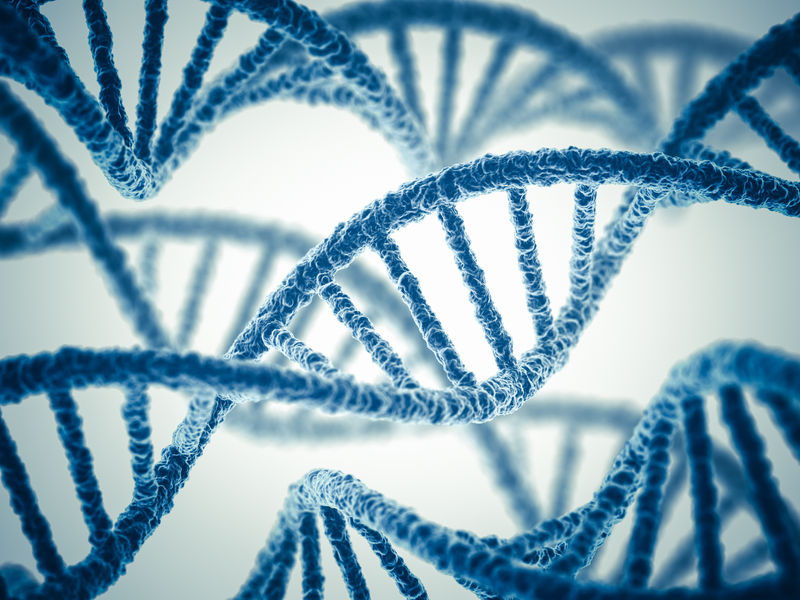
\includegraphics{./figs/DNA-1}
    \caption{\label{fig:fig-DNA-1}DNA}
\end{figure}

\begin{figure}
	\begin{subfigure}{.5\textwidth}
		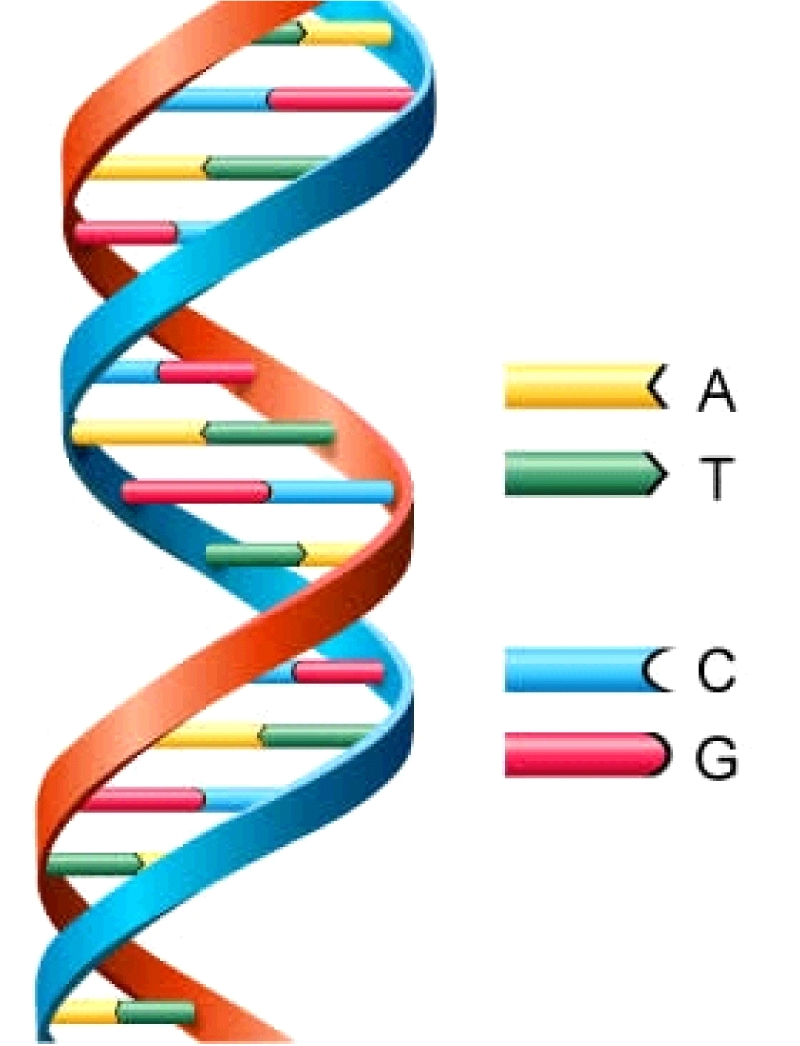
\includegraphics[width=.6\linewidth]{./figs/DNA-2}
	\end{subfigure}
	\begin{subfigure}{.5\textwidth}
		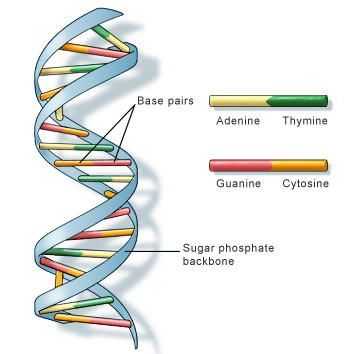
\includegraphics[width=.9\linewidth]{./figs/DNA-3}
	\end{subfigure}
	\caption{\label{fig:fig-DNA-2}DNA scientific analysis}
\end{figure}

An important property of DNA is that it can replicate, or make copies of itself. Each strand of DNA in the double helix can serve as a pattern for duplicating the sequence of bases. This is critical when cells divide because each new cell needs to have an exact copy of the DNA present in the old cell \cite{DNA3}.

\section{DNA Sequencing}
DNA sequence represents a single format onto which a broad range of biological phenomena can be projected for high-throughput data collection \cite{seq1}. 
Over the past years, massively parallel DNA sequencing platforms have become widely available, reducing the cost of DNA sequencing by over two orders of magnitude, and democratizing the field by putting the sequencing capacity of a major genome center in the hands of individual investigators. These new technologies are rapidly evolving, and near-term challenges include the development of robust protocols for generating sequencing libraries, building effective new approaches to data-analysis, and often a rethinking of experimental design (Fig. \ref{fig:fig-NGS-1} and \ref{fig:fig-NGS-2}) \cite{seq2,seq3}.
\begin{figure}
	\centering
	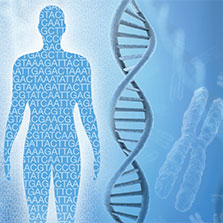
\includegraphics{./figs/NGS-1}
	\caption{\label{fig:fig-NGS-1}DNA sequencing}
\end{figure}

\begin{figure}
	\centerfloat
	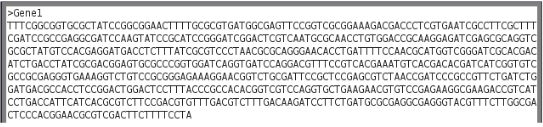
\includegraphics[width=1\linewidth]{./figs/NGS-2}
	\caption{\label{fig:fig-NGS-2}DNA sequencing - Gene example}
\end{figure}

\newpage
One of the core issues of Bioinformatics is dealing with a file formats. Some ad hoc simple human readable formats have over time attained the status of de facto standards. A ubiquitous example of this is the ‘FASTA sequence file format’, originally invented by Bill Pearson as an input format for his FASTA suite of tools.
FASTA format is a text-based format for representing either nucleotide sequences, in which nucleotides are represented using single-letter codes. FASTA format allows for sequence names and comments to precede the sequences. As illustrated in Fig. \ref{fig:fig-NGS-5}, the first line in a FASTA file starts either with a ``\textgreater" (greater-than) symbol or, less frequently, a ``;" (semicolon) and was taken as a comment. Subsequent lines starting with a semicolon would be ignored by software. Since the only comment used was the first, it quickly became used to hold a summary description of the sequence, often starting with a unique library accession number, and with time it has become commonplace use to always use ``\textgreater" for the first line and to not use ``;" comments (which would otherwise be ignored) \cite{fasta-fastq1}.
\begin{figure}
	\centerfloat
	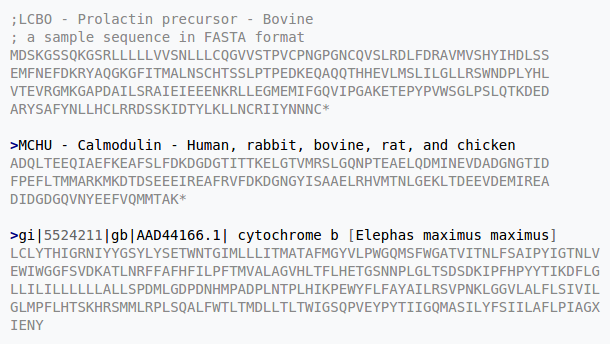
\includegraphics[width=1\linewidth]{./figs/NGS-5}
	\caption{\label{fig:fig-NGS-5}FASTA sample sequences}
\end{figure}
Following the initial line (used for a unique description of the sequence) is the actual sequence itself in standard one-letter code. Anything other than a valid code would be ignored (including spaces, tabulators, asterisks, etc...). Originally it was also common to end the sequence with an ``*" (asterisk) character. 
Over time, this format has evolved by consensus; however, in the absence of an explicit standard some parsers will fail to cope with very long ‘\textgreater’ title lines or very long sequences without line wrapping. There is also no standardization for record identifiers.

In the area of DNA sequencing, the FASTQ file format has emerged as another de facto common format for data exchange between tools. It provides a simple extension to the FASTA format: the ability to store a numeric quality score associated with each nucleotide in a sequence (illustrated in Fig. \ref{fig:fig-NGS-6}) \cite{fasta-fastq2}. 
Early FASTQ uses PHRED quality score \cite{fasta-fastq0} (which is a measure of the quality of the identification of the nucleobases generated by automated DNA sequencing where it is logarithmically linked to error probabilities as illustrated below in Fig. \ref{fig:fig-NGS-3} and \ref{fig:fig-NGS-4}). Storing PHRED scores as single characters (or bytes) gave a simple but reasonably space efficient encoding. In order that the file be human readable and easily edited, this restricted the choices to the ASCII printable characters 32–126 (decimal), and since ASCII 32 is the space character, ASCII 33–126 is used instead to encode PHRED qualities from 0 to 93 (i.e. PHRED scores with an ASCII offset of 33).


\begin{figure}
	\centering
	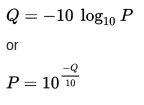
\includegraphics{./figs/NGS-3}
	\caption{\label{fig:fig-NGS-3}Phred quality scores 
	\textit{\textbf{Q}} are defined as a property which is logarithmically related to the base-calling error probabilities \textit{\textbf{P}}}
\end{figure}
\begin{figure}
	\centerfloat
	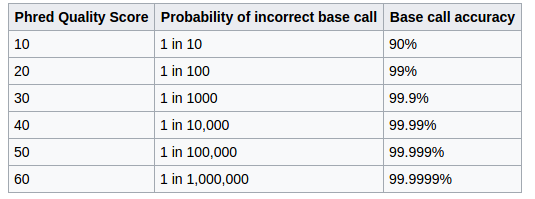
\includegraphics[width=1\linewidth]{./figs/NGS-4}
	\caption{\label{fig:fig-NGS-4}Phred quality scores are logarithmically linked to error probabilities}
\end{figure}

\begin{figure}
	\centerfloat
	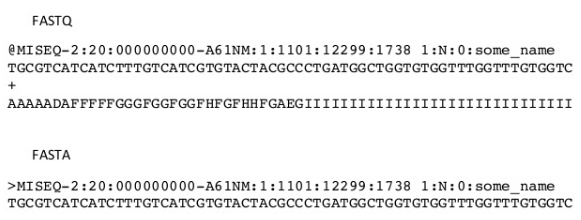
\includegraphics[width=1\linewidth]{./figs/NGS-6}
	\caption{\label{fig:fig-NGS-6}FASTQ VS FASTA}
\end{figure}

\newpage
\section{Next-Generation Sequencing}
As stated above, the field of DNA sequencing technology development has a rich and diverse history. Over the past years, the incentive for developing entirely new strategies for DNA sequencing has emerged on at least four levels, undeniably reinvigorating this field\cite{NGS,NGS1}. First, in the wake of the Human Genome Project, there are few remaining avenues of optimization through which significant reductions in the cost of conventional DNA sequencing can be achieved. Second, the potential utility of short-read sequencing has been tremendously strengthened by the availability of whole genome assemblies for all major model organisms, as these effectively provide a reference against which short reads can be mapped. Third, a growing variety of molecular methods have been developed, whereby a broad range of biological phenomena can be assessed by high-throughput DNA sequencing. And fourth, general progress in technology across disparate fields, including microscopy, surface chemistry, nucleotide biochemistry, polymerase engineering, computation, data storage and others, have made alternative strategies for DNA sequencing increasingly practical to realize. Next-generation DNA sequencing has the potential to dramatically accelerate biological and biomedical research, by enabling the comprehensive analysis of genomes to become inexpensive, routine and widespread, rather than requiring significant production-scale efforts. Since the next-generation sequencing aims to make the vast analysis of genomes less expensive and more spread, it works on enhancing the sequencing time, where too many reads can be generated in a very efficient time. Consequently, it negatively affects the read length and also the sequences accuracy \cite{NGS2}. Actually the next-generation sequencing raises two critical issues, where the first issue is that the read length becomes much shorter than the conventional sequencing, while the second issue is the decrement of the accuracy, where each erroneous nucleotide can be introduced to the read sequence via any of the erroneous actions. There are three erroneous actions are substitution, insertion and deletion illustrated in Fig. \ref{fig:fig-ErrCrr-1}, \ref{fig:fig-ErrCrr-2}, and \ref{fig:fig-ErrCrr-3} respectively. The substitution takes place when the nucleotide is replaced with another erroneous one, while the insertion is when an erroneous nucleotide is newly inserted to the read sequence, and finally the deletion results due to the deletion of a nucleotide from the sequence.

\begin{figure}
	\centerfloat
	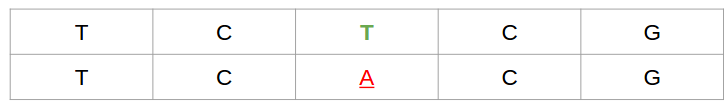
\includegraphics[width=1\linewidth]{./figs/ErrCrr-1}
	\caption{\label{fig:fig-ErrCrr-1}{Substitution Error} - \textbf{T} has been erroneously substituted with \underline{A}}
\end{figure}
\vspace{2cm}
\begin{figure}
	\centerfloat
	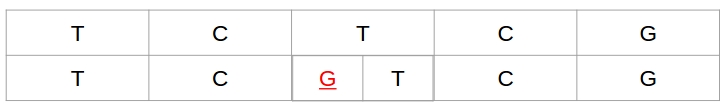
\includegraphics[width=1\linewidth]{./figs/ErrCrr-2}
	\caption{\label{fig:fig-ErrCrr-2}{Insertion Error} - \underline{G} has been erroneously inserted}
\end{figure}
\vspace{2cm}
\begin{figure}
	\centerfloat
	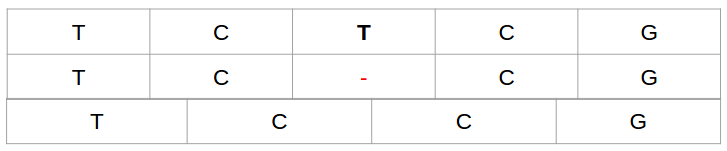
\includegraphics[width=1\linewidth]{./figs/ErrCrr-3}
	\caption{\label{fig:fig-ErrCrr-3}{Deletion Error} - \underline{T} has been erroneously deleted}
\end{figure}


\newpage
\section{NGS Sequences Errors Correction}
The reads accuracy is a vital factor in all reads processes that can be applied to the output reads, like genome assemblers \cite{assembly,assembly1}, and genome aligners \cite{alignment}. For example, the assembly of next-generation sequencing reads can not be accomplished successfully until the reads errors are corrected or eliminated. So detecting and correcting (or eliminating) the reads errors is an essential step that should precede the assembly process. This step can be accomplished either by a standalone solution or implicitly within the assembly mechanism. The nucleotide frequency and its quality value are two main factors that are used in evaluating the nucleotide to erroneous or not \cite{ErrCorr,ErrCorr1}. 

\section{Correction Concepts and Definitions}
There are common concepts and definitions used by most of the corrective algorithms. Most of the corrective algorithms generates all the possible sub-sequences (of length k) from a read, which is called \textit{k-mer} (illustrated in Fig. \ref{fig:fig-CrrConcepts-1}); while the term k-mer frequency represents the number of repetition of a k-mer (a specific sub-sequence of length k) in all the reads. Some of the corrective algorithms set a threshold for the k-mer frequency while classifying the k-mer into strong and weak ones. The strong k-mers are those k-mers that are repeated all over the reads x times, where x is greater than the preset threshold; while the weak k-mers are those ones that are repeated y times all over the reads, where y is less than the k-mer frequency threshold. The filtration step that works on classifying the k-mers into strong and weak ones is called ``Spectrum Alignment". The spectrum alignment depends on the k-mers frequencies and/or the nucleotides quality values.
\\
A de Bruijn graph (illustrated in Fig. \ref{fig:fig-CrrConcepts-2}) can be constructed for any sequence, short or long. The first step is to choose a k-mer size, and split the original sequence into its k-mer components. Then a directed graph is constructed by connecting pairs of k-mers with overlaps between the first k-1 nucleotides and the last k-1 nucleotides. The direction of arrow goes from the k-mer, whose last k-1 nucleotides are overlapping, to the k-mer, whose first k-1 nucleotides are overlapping \cite{deBruijn,deBruijn1}.
\\ 
The number of reads that include a given nucleotide in the sequence is called ``Coverage" \cite{coverage}. The coverage rate of a genome sequences is calculated by the following equation \ref{eq:coverage}
\begin{equation} \label{eq:coverage}
 C = L.N/G 
\end{equation}
where L is the average read length, N is the number of reads and G is the genome length.
\\
Some of the corrective algorithms uses the spectrum alignment in their correction decisions so that the correction takes place by obtaining the nucleotides substitutions that leads to reduce the weak k-mers count by converting them into strong k-mers.
In some other algorithms, the correction takes place using the tree breadth-first search by traversing multi out-going edges nodes, and removing the fewer reads paths, then re-aligns them to the existing path.
\\
There are some corrective algorithms that depends on the reads alignments, where the correction takes place by aligning reads with a common k-mer, then it fixes the misaligned nucleotides based on their occurrences and quality values.
The suffix array also is used in some of the corrective algorithms, where it is built using a string of reads, and the correction takes place with the letter that appears most at each position. Also the suffix trie is used in some other algorithms, where the edges are labelled with DNA letters, while the correction is based on the number of leaves in the sub-trie rooted at the node.
\\
The k-mer hashing table is also used in some corrective algorithms, it is used in storing the total times each nucleotide appears before and after a k-mer, where the error is corrected via the counts. 
\\
Also the k-mer discontinuities is used in some algorithms where the frequencies of adjacent k-mers are calculated and the correction is based on the removal or minimizing the discontinuity.
All of the concepts, stated above, represent the major concepts and paradigms used in the algorithms specialized in correcting the DNA sequencing errors.
\\
The accuracy evaluation of the corrective algorithms depends on calculating some factors as, the true positive rate, the false positive rate, the false negative rate, and the true negative rate. The true positive rate (TP) is the count of the properly corrected nucleotides, while the false positive rate (FP) is the count of the non-erroneous nucleotides that have been corrected improperly. The false negative rate (FN) is the count of the erroneous nucleotides that haven't been detected as erroneous by the algorithm, while the true negative rate (TN) is the count of the non-erroneous nucleotides that have been properly detected as non-erroneous ones. These four factors are the basics factors that are used in calculating the specificity, sensitivity and the accuracy of the algorithm \cite{analysis}. The specificity rate represents the ability of the algorithm to properly corrects the erroneous nucleotides, and it is calculated by the following equation \ref{eq:sensitivity}:
\begin{equation} \label{eq:sensitivity}
  Sensitivity = TP/(TP+FN) 
\end{equation}
While the sensitivity rate represents its ability to detect the erroneous nucleotides, and it is calculated by the following equation \ref{eq:specificity}: 
\begin{equation} \label{eq:specificity}
  Specificity = TN/(TN+FP) 
\end{equation}
And finally the accuracy represents the all over error rate, and it is calculated by the following equation \ref{eq:accuracy}:
\begin{equation} \label{eq:accuracy}
  Accuracy = (TP+TN)/(TP+FP+FN+TN)
\end{equation} 

\newpage
\begin{figure}
	\centerfloat
	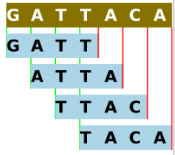
\includegraphics[width=.3\linewidth]{./figs/CrrConcepts-1}
	\caption{\label{fig:fig-CrrConcepts-1}{K-mer} - All the possible sub-sequences (of length k) from a read}
\end{figure}
\vspace{2cm}
\begin{figure}
	\centerfloat
	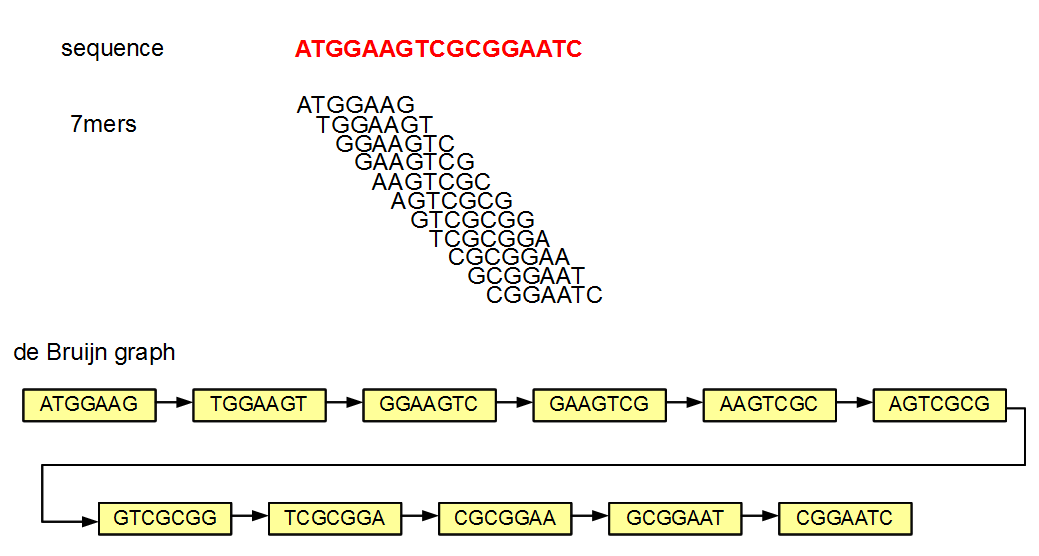
\includegraphics[width=1\linewidth]{./figs/CrrConcepts-2}
	\caption{\label{fig:fig-CrrConcepts-2}{De Bruijn Graph} - k-mer of length 7}
\end{figure}
%

\newpage
\chapter{\label{chap:3}Related Work}
This chapter has two major sections, where it shows the different types of NGS errors correction algorithms, and briefly gives an overview for every existent error correction algorithm.
\\
\\
The error correction methodologies can be either an implicit process within the assembly methodology or a standalone solution that reproduces reads after correction. The assemblers that have embedded error correction are Euler \cite{Euler}, Velvet \cite{Velvet}, AllPaths \cite{AllPaths} and SOAP \cite{Soap}. While the standalone methodologies are Coral \cite{Coral}, Quake \cite{Quake}, Reptile \cite{Reptile}, HSHREC \cite{HShrec}, HiTEC \cite{HiTec}, RACER \cite{Racer}, Pollux \cite{Pollux}, Parallel Error Correction with CUDA \cite{Cuda}, and Error Corrector (EC) \cite{EC}.
\section{Substitution Only Corrective Algorithms}
They are algorithms that are able to correct only the substitution DNA reads errors, these algorithms are: Euler \cite{Euler}, Velvet \cite{Velvet}, AllPaths \cite{AllPaths}, SOAP \cite{Soap}, Quake \cite{Quake}, Reptile \cite{Reptile}, HiTEC \cite{HiTec}, RACER \cite{Racer}, Parallel Error Correction with CUDA \cite{Cuda}, and Error Corrector (EC) \cite{EC}. Check Fig. \ref{fig:fig-RW-1}.
\subsection{Euler}
Euler \cite{Euler} assembly method runs a filtration step called spectrum alignment that aims to classify the k-mers into two categories according to their frequencies all over the reads. Strong k-mers are the ones with high frequencies, while weak k-mers are the ones with lower frequencies. The correction takes place by executing a greedy exploration for base call substitutions aiming to reduce the weak k-mers count.
\\
Since in de novo genome sequencing the sampled genome is not known, EULER uses the number of times a k-mer appears to determine if it is in Gk(the set of k-mers in a genome G), where a threshold M determines whether a k-mer is a solid or a weak one. The read that contains all solid k-mers is referred to as a solid read. Hence, the goal of EULER is to correct the reads so that they are all solid reads.
\\
And the set of all k-mers is updated after each iteration of corrections, so that the reads are deleted if they are not able to be corrected after the last iteration. After then, the assembly of the genome begins after the error correction.
\\
The datasets with low coverage require that the threshold M to be set with a low value so that valid k-mers are not considered weak, but this will cause correct reads to be considered incorrect. 
Where increasing the length of k, will help in reducing the false positive rate and increasing the difficulty of determining the correction changes.
\\
Also in Euler, the reads with erroneous ends are trimmed, because the ends of reads tend to have more errors than the rest of the read, so it's difficult to determine the correct changes to the ends of reads.

\subsection{Velvet}
Velvet's \cite{Velvet} works by efficiently manipulating de Bruijn graphs through simplification and compression, without the loss of graph information, by converging non-intersecting paths into single nodes, i.e. it merges nodes that do not affect the path generated in the graph, so that, whenever a node A has only one outgoing arc that points to node B, with only one ingoing arc, the nodes can be merged.
\\
Velvet eliminates errors and resolves repeats by first using an error correction algorithm that merges sequences together. Repeats are then removed from the sequence via the repeat solver that separates paths which share local overlaps.
\\
\\
In other words, velvet's tour bus algorithm uses breadth-first search (BFS), starting at nodes with multiple out-going edges, where candidate paths are traversed in step, moving ahead one node on all paths per iteration, until the path lengths exceed a threshold. Velvet removes the path representing fewer reads then re-aligns reads from the removed path to the remaining path.

\subsection{AllPaths}
AllPaths \cite{AllPaths} uses a read-correcting preprocessor related to the spectral alignment in Euler, where the reads filtration is based on quality values, which is further used in correcting some substitutional errors. 

\subsection{SOAP}
SOAP \cite{Soap} filters and corrects reads using pre-set thresholds for k-mer frequencies. It removes bubbles with an algorithm like Velvet's tour bus, with higher read coverage determining the surviving path (read).

\subsection{Quake}
Quality-aware Detection and Correction of Sequencing Errors (Quake) \cite{Quake} determines a cut-off value which separates trusted k-mers from untrusted k-mers, using the distribution of k-mers based on their quality scores. The intersection of the untrusted k-mers is used to localize the search for an error in a read. Quake tries to evaluate the conditional probability of assigning the actual nucleotides of the sequenced fragment, given the observed nucleotides.
\\
It relies on k-mer coverage and quality scores to correct reads, as it uses a method of evaluating the quality of a k-mer based on the associated quality scores for each base. 
\\
The k-mers weighing is based on quality scores, where the low coverage true k-mers will have high quality scores and the high coverage k-mers with errors will have low quality scores.
\\
Quake begins by counting all the k-mers in the dataset, so the value of k, has a significant impact on the performance of Quake. But actually for an appropriate choice for k, Quake uses the following equation \ref{eq:quake-k} to set k (where G is the size of the genome).
\begin{equation} \label{eq:quake-k}
 k \approx log_{4} 200G  
\end{equation}
After then, it determines a cut-off value which separates trusted k-mers from untrusted k-mers, using the distribution of k-mers based on their quality values, where the reads with untrusted k-mers are considered for correction, and the errors are detected based on the intersection of the untrusted k-mers, which is used to localize the search for an error in a read. 
\\
Actually, Quake considers every base covered by the right most trusted k-mer, and left most trusted k-mers to be correct, so if the errors are near the end of a read, it will be checked first whether it is in the right most or left most, after then the decision will be taken. Also it tries to evaluate the conditional probability of a assigning the actual nucleotides of the sequenced fragment, given the observed nucleotides.
\\
\\
Quake has some heuristics, like ambiguous true correction, where the repeats implies to having multiple sets of valid corrections, with a small difference in the likelihood of each correction, so a true correction is ambiguous. So, it continues past the threshold to ensure that another valid set does not exist. 
\\
Quake stops correcting if the region is filled with low quality scores, where the reads with a region containing $\geq$ 13 positions with a probability of error $>$ 1\% are not corrected. And the reads with regions containing $\geq$ 9 positions with a probability of error $>$ 1\%, the likelihood ratio threshold is increased to $10^{-3}$.
\subsection{Reptile}
Representative Tiling for Short Read Error Correction (Reptile) \cite{Reptile} uses the spectral alignment approach used in Euler, with the quality score information if available. Trying to create approximate multiple alignments by considering all reads with pairwise hamming distance less than a pre-set threshold. 
\\
\\
Reptile considers all reads with pairwise Hamming distance less than a set threshold, where it finds the multiple alignments by only aligning k-mers in the reads. Actually, it chooses the size of k so that the expected number of occurrences of any k-mer in the genome should be no more than one. And it uses contextual information to help resolve errors without increasing k.
\\
\\
The main disadvantage of Reptile is that the user have to set the parameters, so it
requires running scripts and analyzing the results to obtain the proper parameters.

\subsection{HiTEC}
High Throughput Error Correction (HiTEC) \cite{HiTec} uses a suffix array that is built using a string of reads and their reverse complements. The correction of an erroneous nucleotide takes place with the letter that appears most at that position.
\\
\\
HiTec uses the suffix array as it is a more time and space efficient data structure than the suffix trie, where it uses an array that stores the length of the longest common prefix (LCP) between consecutive suffixes in the suffix array.
\\
\\
Actually, it assumes that the length of the genome and the error rate of the dataset is supplied. Also HiTEC assumes that a read, starting at position j of the genome, contains an error in position m and that the previous w positions, $r_{i} [m - w..m - 1]$, are correct.
\\
As the length of witness length (w) decreases:

\begin{itemize}
	\item The number of uncorrectable reads U(w) decreases.
	\item The probability of seeing the witness increases, so the correct positions changed incorrectly. 
	\item The number of destructible reads D(w) increases.
	\item A value for w must be found that minimizes U(w)+ D(w). 
\end{itemize}

So, HiTEC uses a variation of witness lengths based on the optimal witness length to achieve high accuracy.
\\
\\
After then, HiTEC uses the majority of one base at a position, the erroneous base is changed to the base that appears most at that position. If there is no ambiguity in the correct letter then the correction is made. But, if there is ambiguity, then the next two letters are checked in order to decide how to correct the read. And finally, it stops correcting when the number of bases changed during one iteration is less than 0.01\% of the total number of bases, or after nine iterations or corrections.
\\
\\
HiTEC only requires modest coverage to make corrections. So, the datasets with high coverage are split into several sets with lower coverage that are independently corrected. 
\\
\\
The disadvantages of HiTEC can be listed as:
\begin{itemize}
	\item It does not correct reads with ambiguous letters.
	\item It can only correct datasets if the reads are all the same length.
	\item It does not run in parallel mode.
\end{itemize}

\subsection{RACER}
Rapid and Accurate Correction of Errors in Reads (RACER) \cite{Racer} is able to correct datasets that have varying read lengths. Using a hash table that stores the total times each nucleotide appears before and after each k-mer, where the error is corrected via the counts.
\\
\\
Actually, RACER replaces the suffix array approached used in HiTEC with a more time and space efficient hash table. And as stated above, this hash table stores the k-mers in each read, and the total times each base appears before and after each k-mer. While, the optimal k-mer length is calculated with a similar statistical analysis as HiTEC, i.e, it's value must be found that minimizes U + D, where U is the number of uncorrectable reads and D is the number of destructible reads. In other words, it choose k that will minimize the number of false positives and maximize the number of corrections. And after the k-mers and the counters have been calculated, the reads are corrected based on the counts.
\\
\\
RACER encodes the input sequences using two bits to represent each base, where the k-mer and its reverse complement must be searched, and only the one with the smaller encoding key is stored. Consequently, it shows a great enhancement in time and memory usage, where there is no algorithm can beat RACER in time.
\\
One more significant advantage of RACER is that it is able to correct datasets that have varying read lengths, and runs in both serial and parallel mode.
 

\subsection{Parallel Error Correction with CUDA}
Parallel Error Correction with Compute Unified Device Architecture (CUDA) \cite{Cuda} uses the spectrum alignment besides a voting algorithm for the single-mutation using each letter, hence errors can be fixed based on high values in the voting matrix.
\\
\\
CUDA (Compute Unified Device Architecture) is an extension of C/C++ to write scalable multi-threaded programs for CUDA-enabled GPUs, where CUDA programs can be executed on GPUs with NVIDIA’s Tesla unified computing architecture, while CUDA programs contain a sequential part, called a kernel.
\\
\\
CUDA uses the single-mutation voting algorithm, where it firstly initialize the voting matrix by zeros for each of (A, C, T, G) for every nucleotide, and loop on every read to check whether it is in the spectrum or not. If it found that the read is not in the spectrum, it loops on every nucleotide against its voting matrix and increase the vote by 1 for every successful replacement (that makes the reads fit into the spectrum). After then the errors can be fixed based on high values in the voting matrix.
\subsection{Error Corrector}
Error Corrector (EC) \cite{EC} an error correction algorithm for correcting short reads with substitution errors only. Using k-mers hashing tables to find the neighbours of each of the reads, where each read is corrected using its neighbours.
\\
\\
In other words, the steps of Error Corrector (EC) can be broken into three independent tasks. At first it builds k-mers and hashes the k-mers into hash tables. After then, by using these hash tables it finds the neighbours of each of the reads. And finally, each read is then corrected using the neighbours of the read.

\begin{figure}
	\centerfloat
	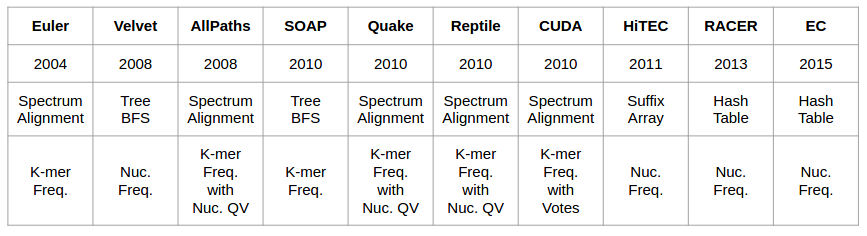
\includegraphics[width=1.35\linewidth]{./figs/RW-1}
	\caption{\label{fig:fig-RW-1}An illustrative summary for the substitution only corrective algorithms}
\end{figure}


\section{Substitution, Insertion And Deletion Corrective Algorithms}
They are algorithms that are able to correct all types of DNA reads errors, these algorithms are: Coral \cite{Coral}, HSHREC \cite{HShrec}, and Pollux \cite{Pollux}. Check Fig. \ref{fig:fig-RW-2}

\subsection{Coral}
Correction with Alignments (Coral) \cite{Coral} is able to correct all types of errors (substitution, insertion and deletion). The methodology is built on scoring the alignments between short reads, where each alignment runs on a base read with all the reads that have at least one common k-mer with this base read. Then the correction takes place for the misaligned positions depending on the number of times each letter occurs in addition to quality scores of the nucleotide.
\\
Coral uses multiple sequence alignments (MSA) \cite{coral-alignment} between short reads to detect errors, where the calculates the gap penalty and mismatch penalty (parameters for scoring the alignments) have a significant impact on the quality of the corrections. 
\\
The main defect in Coral is that it isn't able to correct mixed datasets that contain both substitution errors with insertion and deletions ones.
For substitution errors, Coral sets the gap penalty with a very high value to prevent insertions and deletions in the alignments. While for insertion and deletion errors, Coral sets the gap and mismatch penalties to be equal.
\\
Coral can summarize his algorithm as:
\begin{enumerate}
	\item Indexing Reads, where a hash table is used to store the k-mers and the reads that contain each k-mer. And in order to save space, Coral store the information of only the lexicographically smaller of the k-mer \& its reverse. It also does not store any k-mers that contain ambiguous letters.
	\item Multiple Alignments, where Coral starts each alignment with one read which is called the base read, and all the reads that share at least one k-mer with the base read are found using the k-mer hash table, and they are called neighbourhood of the base. If the neighbourhood of the base read is very large or very small, then Coral does not perform any alignments.
 As, if it's very large, then the reads likely came from different regions in the genome and the MSA will take a long time to compute, as the alignments will be very poor. But, if it's very small, then there is likely not enough coverage to make any significant corrections.
\\
Coral doesn't correct the reads that have been corrected before. So, if a read has already been corrected in a previous alignment, Coral tries to align it to the consensus without errors in the region of the k-mer. And, if a read aligns perfectly to the consensus then the rest of the read is not aligned to save time. But, if a read has many errors compared to the consensus then it stops aligning the read and moves on to the next one. And if the gaps are not allowed then a gap-less alignment is performed between a read and the consensus sequence.

\item Correcting Reads, where Coral calculates the number of misaligned positions for each read compared to the consensus sequence. And if the quality of the alignment is above a preset threshold, then it will be used to correct the aligned reads. The support threshold for each position in the consensus sequence is calculated as: (num of times each letter occurs)/ (total num of reads aligned at that position). In case a read differs from the consensus at any position, then the letter is changed in the read provided the support is above the threshold. And if quality scores are available and there is a gap in an aligned read, then:
 quality score of the gap = avg (the quality scores of the bases flanking the gap).
\end{enumerate}
The complexity of Coral is illustrated as follow (assuming that where M is the combined total length of the reads, L is the maximum number of reads in a neighbourhood, and r is the longest read length):
\begin{itemize}
	\item If gaps are allowed, the worst case runtime is O(MrL).
	\item If only mismatches are allowed, the worst case runtime is O(ML).
	\item The space for the hash table that stores the k-mers is bounded by O(M).
	\item The space complexity for computing the MSA is O(Lr + r\textsuperscript{2}).
	\item The overall space complexity is O(M).
\end{itemize}

\subsection{HSHREC}
Hybird Short Read Error Correction (HSHREC) \cite{HShrec} is able to correct all types of errors (substitution, insertion and deletion). The methodology depends on the alignment of a read with others using a suffix trie, where the edges are labelled with DNA letters and a node weight is the number of leaves in the sub-trie rooted at that node. On the down levels, a node with more than one child is considered to have a substitution error, while extra branching in the generalized suffix trie is caused by insertion and deletion erroneous actions.
\\
\\
SHREC was designed to correct substitution errors, and HSHREC is able to correct both substitution errors and insertion and deletion erroneous actions.
\\
HSHREC assumes that the input contains k reads randomly sampled from a genome with read length n, where n can vary in length. The errors are detected in a read by aligning it to the other reads using a suffix trie, where the erroneous region of the read has a low weight in the trie and this is the area that will be corrected.
\\
\\
HSHREC resolves the ambiguity that can be caused by single nucleotide polymorphisms (SNPs). The single nucleotide polymorphisms (SNPs) is the phenomena of changing single nucleotide that differ between individuals of the same species, and they can appear as errors. Actually, SNPs are the most abundant type of genetic marker and their high density makes them ideal for studying the inheritance of genomic regions \cite{SNP1,SNP2}, so its discovery and genotyping are essential to genetic mapping. There remains a need for a simple, inexpensive platform that allows high-density SNP discovery and genotyping in large populations \cite{SNP3}. But HSHREC analyse it as: since the errors at the SNP location will only be in a few reads, and SNPs will be present in several reads, it is possible to differentiate them.
\\
\\
In HSREC, each read has a unique suffix by concatenating a unique number from 1 to 2k to the end of each string in R (the set of reads, and their reverse complements). And the edges of the trie are labeled with DNA letters, and an ambiguous letter N, where the concatenation of edge labels from the root to a node is called a path-label. 
\\
For any suffix of a string in R, there is a path-label that contains that suffix. And the weight of a node in the trie is the number of leaves in the subtrie that is rooted at that node, and is the number of suffixes in that subtrie. 
\\
The level of a node is the length of the path from the root to the node. In the top levels of the trie almost all nodes have four or five children. while in the down levels of the trie almost all nodes have only one child. So, if a child at down levels has more than one child then it is likely an error, and the node with the lower weight is likely the erroneous base. 
\\
So, HSHREC algorithm traverses the trie to identify errors at the intermediate levels of the trie. And it tries to correct each error with a substitution, and the remaining errors are treated as insertions or deletions.
\\
In SHREC, it compares the subtrie rooted at the low weight node to the subtries rooted at the siblings of the node, while the insertion and deletion erroneous actions cause extra branching in the generalized suffix trie. The insertion erroneous action creates a low weight node, so the deletion corrective action of the node causes the children rooted at the node and their siblings to be merged. And a comparison of the subtries before and after the deletion determine if the deletion is a proper way to correct the node or not. 

\subsection{Pollux}
Platform Independent Error Correction of Single and Mixed Genomes (Pollux) \cite{Pollux} calculates the k-mer frequencies in the entire set of reads. Identifying the discontinuities by comparing the frequencies of adjacent k-mers within reads, assuming that individual k-mers are not erroneous. The discontinuities within reads are used to find error locations and evaluate correctness. The correction is chosen to be the one that removes or minimizes the k-mer count discontinuity.
\\
\\
Pollux decomposes each read into k-mers and then calculates the k-mer frequencies in the entire set of reads. The nucleotide is represented with a two-bit alphabet and a hash-table strategy is used to help in using large k-mers (with length 31) to avoid common short repeats which might otherwise confound the correction procedure.
\\
\\
Firstly it identifies the individual k-mers as not erroneous, then identifies the discontinuities by comparing the frequencies of adjacent k-mers within reads. The discontinuities within reads are used to find error locations and evaluate correctness. A read that is not erroneous is assumed to have a k-mer count profile that is reflective of a random sampling process, given local coverage. In contrast, a read that contains an error is likely to have k-mer counts that deviate unexpectedly from this random process. Evaluating multiple k-mers containing bases following the erroneous base to ensure our correction is appropriate. The correction is chosen to be the one that removes or minimizes the k-mer count discontinuity. If there exist multiple corrections which achieve this, the correction is chosen to be the one that improves the most k-mer counts maximally beyond the current erroneous location. Pollux corrects each read independently and does not update recorded k-mer counts as a result of correction.
 
\begin{figure}
	\centerfloat
	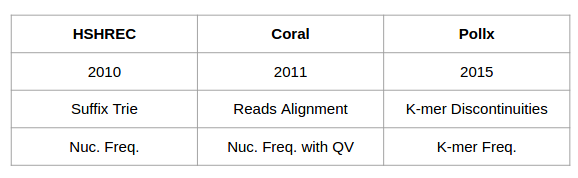
\includegraphics[width=1\linewidth]{./figs/RW-2}
	\caption{\label{fig:fig-RW-2}An illustrative summary for the substitution, insertion and deletion corrective algorithms}
\end{figure}

\newpage
\chapter{\label{chap:4}K-mer Grouping Error Correction Algorithm}
This chapter illustrates the working methodology of K-mer Grouping Error Correction (KGEC - the first proposed algorithm) in details, where the pseudo code, diagram and examples are discussed in details. While the evaluation will be discussed in chapter \ref{chap:6}.
\\
\\
The first proposed algorithm (Kmer Grouping for Error Correction or KGEC) aims to correct all types of errors and to raise the next-generation sequencing output accuracy. It tries to compete in the accomplishment time with the currently existent algorithms specialized in correcting all types of the errors found in the output of the next-generation sequencing, i.e. the substitution erroneous actions, the insertion erroneous actions and the deletion erroneous actions). Also it has the flexibility to run more than a correction iteration, which usually helps in enhancing the accuracy.
\section{\label{sec:alg1-meth}Methodology}
As stated before, this algorithm aims to correct all types of errors (substitution, insertion and deletion). It mainly depends on k-mers grouping. So, firstly it builds a hash table that maps the k-mer into integer and saves its frequency all over the reads. The hashing algorithm (illustrated in Fig. \ref{fig:fig-KGEC-HASH}) is inherited from Coral \cite{Coral}, where the k-mer and its complement will map to the same integer. Then, it groups k-mer based on having same nucleotides in the same order, with a mutation in the first, middle and last positions. After then, each k-mer group will search for the k-mer with the highest frequency to use it in unifying all of the rest of the group members (k-mers) to make them all have the same nucleotides in the same order of the k-mer with the highest frequency. In case of having more than a k-mer having the same highest frequency within the same group, the algorithm searches for the one with the highest frequency and highest quality value average of its nucleotides, where the quality value of the nucleotide in the k-mer is calculated as the average of the quality value of this nucleotide in the reads that have this k-mer as a subsequent. 
\\
\\
After correcting the k-mer groups with their best k-mer, it checks those k-mers that does not belong to any group and consequently is not corrected yet, and tries to re-group them again but this time based on having same nucleotides in the same order, with a mutation in the three positions of the nucleotides that have lowest three quality values compared to the rest of the nucleotides within the same k-mer. And similarly, each k-mer group will search for the k-mer with the highest frequency to use it in unifying all of the rest of the group members (k-mers) to make them all have the same nucleotides in the same order of the k-mer with the highest frequency (and highest quality value average if needed). 
\\
Check the illustrative example shown in Fig. \ref{fig:fig-KGEC-EX} and the diagram shown below in Fig. \ref{fig:fig-First-Proposal-1}. Also the pseudo-code of the hashing algorithm and that of the correction are illustrated in Fig. \ref{fig:fig-KGEC-HASH} and Fig. \ref{fig:fig-KGEC-ALG} respectively.
\\
\\
Finally, the algorithm corrects the reads with corrected k-mers, where it decides the corrective action (substitution, insertion and deletion) based on the studying the erroneous nucleotide and its neighbours (similarly to H-RACER correction action procedure, so it will be explained in details in the following chapter). After this step, it will repeat the flow again if it was running in iterative mode (set by a given parameter that sets the iterations count).

\begin{figure}
\vspace{0cm}
\begin{bordered}
\begin{enumerate}
	\item \underline{Extracted K-mers with Frequencies}
	\begin{enumerate}
		\item CCGTAAT - Freq. = 9
		\item CGCTACT - Freq. = 13
		\item GTACGGT - Freq. = 8
		\item AGCTACT - Freq. = 4
		\item GTCCTGT - Freq. = 3
		\item ACGTAAT - Freq. = 2
		\item GGCCACT - Freq. = 2
		\item GGCCTAA - Freq. = 1
		\item TGCCACC - Freq. = 3
	\end{enumerate}
	\item \underline{K-mers Grouping (\textit{0, (k-1)/2, k})}
	  \begin{enumerate}
		\item \underline{CCGTAAT} \hspace{1.8ex}- Freq. = 9
		\item \textbf{CGCTACT} - Freq. = 13
		\item GTACGGT \hspace{1.8ex}- Freq. = 8
		\item \textbf{AGCTACT} - Freq. = 4
		\item GTCCTGT \hspace{1.8ex}- Freq. = 3
		\item \underline{ACGTAAT} \hspace{1.8ex}- Freq. = 2
		\item \textbf{GGCCACT} - Freq. = 2
		\item GGCCTAA \hspace{1.8ex}- Freq. = 1
		\item \textbf{TGCCACC} - Freq. = 3
	  \end{enumerate}
	  Hence, there are two groups formed:
	\begin{itemize}
	  \item 
	  \begin{enumerate}
		\item \underline{C}\textbf{CG}\underline{T}\textbf{AA}\underline{T} - Freq. = 9
		\item \underline{A}\textbf{CG}\underline{T}\textbf{AA}\underline{T} - Freq. = 2
	  \end{enumerate}
	\end{itemize}
	\begin{itemize}
	  \item 
	  \begin{enumerate}
		\item \underline{C}\textbf{GC}\underline{T}\textbf{AC}\underline{T} - Freq. = 13
		\item \underline{A}\textbf{GC}\underline{T}\textbf{AC}\underline{T} - Freq. = 4
		\item \underline{G}\textbf{GC}\underline{C}\textbf{AC}\underline{T} - Freq. = 2
		\item \underline{T}\textbf{GC}\underline{C}\textbf{AC}\underline{C} - Freq. = 3
	  \end{enumerate}
	\end{itemize}
	While the remaining with no group are:
	\begin{itemize}
		\item GTACGGT - Freq. = 8
		\item GTCCTGT - Freq. = 3
		\item GGCCTAA - Freq. = 1
	\end{itemize}
	\item \underline{Correcting K-mer Groups}
     \begin{itemize}
	  \item Corrective: \underline{C}\textbf{CG}\underline{T}\textbf{AA}\underline{T} - \textbf{Freq. = 9}
	  \begin{enumerate}
		\item \underline{A}\textbf{CG}\underline{T}\textbf{AA}\underline{T} - Freq. = 2
	  \end{enumerate}
	\end{itemize}
	\begin{itemize}
	  \item Corrective: \underline{C}\textbf{GC}\underline{T}\textbf{AC}\underline{T} - \textbf{Freq. = 13}
	  \begin{enumerate}
		\item \underline{A}\textbf{GC}\underline{T}\textbf{AC}\underline{T} - Freq. = 4
		\item \underline{G}\textbf{GC}\underline{C}\textbf{AC}\underline{T} - Freq. = 2
		\item \underline{T}\textbf{GC}\underline{C}\textbf{AC}\underline{C} - Freq. = 3
	  \end{enumerate}
	\end{itemize}
	\item \underline{K-mers (\textit{weakest 3 nucleotides})}
	\begin{itemize}
		\item 
	Hence, one group is formed \textit{assuming weakest 3 nucleotides of GTACGGT are the three middles}
		\begin{enumerate}
		\item GT\underline{A}\underline{C}\underline{G}GT - \textbf{Freq. = 8}
		\item GT\underline{C}\underline{C}\underline{T}GT - Freq. = 3
		\end{enumerate}
	\end{itemize}
	\item \underline{Correcting K-mers Groups}
	\begin{itemize}
		\item GT\underline{A}\underline{C}\underline{G}GT - \textbf{Freq. = 8}
		\begin{enumerate}
		\item GT\underline{C}\underline{C}\underline{T}GT - Freq. = 3
		\end{enumerate}
	\end{itemize}
\end{enumerate}
\end{bordered}
\caption{\label{fig:fig-KGEC-EX}KGEC Grouping and Correction Decision Examples}
\end{figure}

\begin{figure}
	\centerfloat
	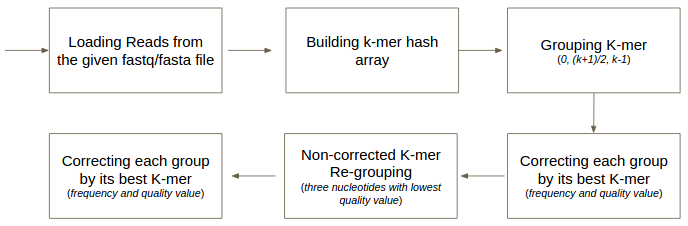
\includegraphics[width=1.6\linewidth]{./figs/First-Proposal-1}
	\caption{\label{fig:fig-First-Proposal-1}KGEC Diagram}
\end{figure}

\begin{figure}
\vspace{0.1cm}
\begin{bordered}
Assume a read represented as: $r=s_1s_2\cdots s_n$
\\
Assume k represents the k-mer length
\\
Set code\_a with 0x00
\\
Set code\_c with 0x01
\\
Set code\_g with 0x02
\\
Set code\_t with 0x03
\\
Set gram as uint64\_t with zero value
\\
Set gram\_reverse as uint64\_t with zero value
\\
Set mask as uint64\_t with ((uint64\_t) 1 $<<$ (2 * k)) - 1
\\
Set pre\_gram as uint64\_t with zero value
\\
Set pre\_mask as uint64\_t with zero value
\\
Set lastPos with -1
\\
\\
For every nucleotide $s_i$ in $r$ 
\begin{enumerate}
\addtolength{\itemindent}{1cm} 
\item Check the value of $s_i$, if: 
\vspace{-2mm}
\begin{enumerate}
\addtolength{\itemindent}{1cm}

	\item if $s_i$ equals `A' or `a'
	
	\noindent\hspace{1cm}then,
	
	\begin{itemize}
    \addtolength{\itemindent}{1cm}
	  \item Reset gram with: gram $<<$ 2 $|$ code\_a
      \item Reset gram\_reverse with: gram\_reverse $>>$ 2 $|$ code\_t $<<$(k - 1)*2
	\end{itemize}
	
	\item if $s_i$ equals `C' or `c'
	
	\noindent\hspace{1cm}then,

	\begin{itemize}
    \addtolength{\itemindent}{1cm}
	  \item Reset gram with: gram $<<$ 2 $|$ code\_c
	  \item Reset gram\_reverse with: gram\_reverse $>>$ 2 $|$ code\_g $<<$(k - 1)*2
	\end{itemize}
	
	\item if $s_i$ equals `G' or `g'
	
	\noindent\hspace{1cm}then,

	\begin{itemize}
    \addtolength{\itemindent}{1cm}	
     	\item Reset gram with: gram $<<$ 2 $|$ code\_g
      	\item Reset gram\_reverse with: gram\_reverse $>>$ 2 $|$ code\_c $<<$(k - 1)*2
	\end{itemize}
	
	\item if $s_i$ equals `T' or `t'
	
	\noindent\hspace{1cm}then,

	\begin{itemize}
    \addtolength{\itemindent}{1cm}
      \item Reset gram with: gram $<<$ 2 $|$ code\_t
	  \item Reset gram\_reverse with: gram\_reverse $>>$ 2 $|$ code\_a $<<$(k - 1)*2
	\end{itemize}

\end{enumerate}

\item Reset gram with: gram \& mask

\item Reset gram\_reverse with: gram\_reverse \& mask;

\item Check if $i >$ k, then, check:
\vspace{-2mm}
\begin{enumerate}
\addtolength{\itemindent}{1cm}
      \item if gram $<$ gram\_reverse \&\& (gram \& pre\_mask) == pre\_gram
      	
      \noindent\hspace{1cm}then, add a k-mer to the hash array at index mapped to gram
	   
	  \item if gram\_reverse $<$ gram \&\& (gram\_reverse \& pre\_mask) == pre\_gram
	  
      \noindent\hspace{1cm}then, add a k-mer to the hash array at index mapped to gram\_reverse
	  
\end{enumerate}            
End For	
\end{enumerate}
\end{bordered}
\caption{\label{fig:fig-KGEC-HASH}KGEC K-mer Hashing Abstraction}
\end{figure}

\begin{figure}
\vspace{0.1cm}
\begin{bordered}
Assume kmer\_hash\_arr is an array that hold the hashing table  with length m
\\
Assume k represents the k-mer length
\\
\\
For every k-mer in kmer\_hash\_arr

\noindent\hspace{0.4cm} Check if this k-mer doesn't belong to any k-mer group

\noindent\hspace{0.4cm} then,

\vspace{-3mm}
\begin{enumerate}
\addtolength{\itemindent}{1cm}
	  \item Initialize a new k-mer group

	  \item Add this k-mer to the new k-mer group

      \item Generate all k-mers having typical nucleotides as this k-mer, except,
      
      \noindent\hspace{1cm} for these positions \{0, (k-1)/2, k-1\}, it may have different nucleotide
      
      \item For every generated k-mer
	
		\noindent\hspace{1.4cm} if the hash of this generated k-mer existent in kmer\_hash\_arr 
		
		\noindent\hspace{1.4cm} then, add this generated k-mer to the new k-mer group created above
		
		\noindent\hspace{1cm} End For

\end{enumerate}            
\vspace{-3mm}

End For
\\
\\
For every k-mer group 

\vspace{-3mm}
\begin{enumerate}
\addtolength{\itemindent}{1cm}
  \item Search for the k-mer with the highest frequency 

  \item Check if there are more than one k-mer having the highest frequency

  \noindent\hspace{1cm} then, set corrective\_kmer as the one with the highest frequency and quality

  \noindent\hspace{1cm} else, set corrective\_kmer as the one with the highest frequency

  \item For every k-mer in this k-mer group

  \noindent\hspace{1.4cm}Mark this k-mer's nucleotides at \{0, (k-1)/2, k-1\} to be corrected 
  
  \noindent\hspace{1.4cm}with their corresponding one in the corrective\_kmer
  
  \noindent\hspace{1cm} End For
\end{enumerate}            
\vspace{-3mm}

End For
\\
\\
For every k-mer in kmer\_hash\_arr

\noindent\hspace{0.4cm} Check if this k-mer doesn't belong to any k-mer group

\noindent\hspace{0.4cm} then,

\vspace{-2mm}
\begin{enumerate}
\addtolength{\itemindent}{1cm}
	  \item Set weak\_positions array to hold the position of the three nucleotides with 
	  
	  \noindent\hspace{1cm}the lowest quality
	  
	  \item Initialize a new k-mer group

	  \item Add the weak\_positions element to the new k-mer group

	  \item Add this k-mer to the new k-mer group

      \item Generate all k-mers having typical nucleotides as this k-mer, except,
      
      \noindent\hspace{1cm} for the positions in weak\_positions, it may have different nucleotide
      
      \item For every generated k-mer
	
		\noindent\hspace{1.4cm} if the hash of this generated k-mer existent in kmer\_hash\_arr 
		
		\noindent\hspace{1.4cm} then, add this generated k-mer to the new k-mer group created above
		
		\noindent\hspace{1cm} End For

\end{enumerate}            
\vspace{-3mm}
End For
\\
\\
For every k-mer group 
\vspace{-3mm}
\begin{enumerate}
\addtolength{\itemindent}{1cm}
  \item Search for the k-mer with the highest frequency 

  \item Check if there are more than one k-mer having the highest frequency

  \noindent\hspace{1cm} then, set corrective\_kmer as the one with the highest frequency and quality

  \noindent\hspace{1cm} else, set corrective\_kmer as the one with the highest frequency

  \item For every k-mer in this k-mer group

  \noindent\hspace{1.4cm}Mark this k-mer's nucleotides at the weak\_positions element of this    
  
  \noindent\hspace{1.4cm}k-mer group to be corrected with their corresponding one in the 
  
  \noindent\hspace{1.4cm}corrective\_kmer
  
  \noindent\hspace{1cm} End For
\end{enumerate}            
\vspace{-3mm}
End For		
\end{bordered}
\caption{\label{fig:fig-KGEC-ALG}KGEC Grouping and Correction Decision Pseudo-Code - O(\textit{$4^m$})}
\end{figure}


\chapter{\label{chap:5}H-RACER Algorithm}
This chapter illustrates the working methodology of H-RACER (the second proposed algorithm) in details, where the pseudo code, flowchart and examples are discussed in details. While the evaluation will be discussed in chapter \ref{chap:6}.
\\
\\
The second proposed algorithm (Hybird RACER or H-RACER) is the newly proposed algorithm that aims to correct all types of errors. H-RACER follows the same algorithm of RACER in detecting errors and deciding their corrections, the newly added part in H-RACER is the detection of the error type in order to apply the correction properly for datasets with varying error types.

\section{Methodology}
As stated before, H-RACER aims to correct all types of errors (substitution, insertion, and deletion). Although RACER is the fastest DNA error correction algorithm existent nowadays with a high accuracy, but it can not correct all types of errors, it can only correct substitutions. So, H-RACER is proposed in order to correct all types of errors. Hence, it follows the same algorithm of RACER in detecting errors and deciding their corrections, and the newly added part is the detection of the error type in order to apply the correction properly for datasets with varying error types.
\\
\\
H-RACER detects the error type for an erroneous nucleotide by studying its correction value (obtained by RACER) against its neighbours, then decides the corrective action (substitute, insert, delete) according to the detected error type.
Once the error detection and correction stages are done, H-RACER starts applying correction using its own methodology which mainly depends on detecting the error type in order to apply the detected correction with the proper action (substitution, insertion or deletion).
\\
\\
H-RACER starts the error type detection by looping on every nucleotide in the whole reads set, to check if this nucleotide is an erroneous one. For every erroneous nucleotide H-RACER checks the position of this nucleotide in the read not to be the last one in the read (so that there is at least one nucleotide following it) where the follower nucleotide is erroneous too. Then H-RACER starts to examine the erroneous and corrective values for both nucleotides (the current and its follower). H-RACER checks if the correction value of the current erroneous nucleotide is equal to the erroneous value of its follower, so it will be concluded that this current erroneous nucleotide is a result of an insertion erroneous action. Hence, H-RACER applies the correction as a deletion action for this current erroneous nucleotide. But, if it is found that the erroneous value of the current nucleotide is equal to the correction value of its erroneous follower, so it will be concluded that this current erroneous nucleotide is a result of a deletion erroneous action. Hence, H-RACER applies the correction as an insertion action at a position directly before the current erroneous nucleotide with the correction value of it (the current erroneous nucleotide). Otherwise, if there is not any criss-cross equality relation between the erroneous and correction values of the current nucleotide and its erroneous follower (i.e. the correction/erroneous value of the current erroneous nucleotide is not equal to the erroneous/correction value of its follower), then it will be concluded that this current erroneous is a result of a substitution erroneous action. Hence, H-RACER applies the corrective action as a substitution action for the erroneous value of the current nucleotide with its correction value.
\\
\\
On another side, if it is found that the current nucleotide is the last one in the read or its follower nucleotide is not erroneous, then H-RACER will check the position of this nucleotide in the read not to be the first in the read (so that there is at least one nucleotide that precedes it) where the precedent nucleotide is erroneous too. Then H-RACER starts to examine the erroneous and corrective values for both nucleotides (the current and its precedent). H-RACER checks if the correction value of the current erroneous nucleotide is equal to the erroneous value of its precedent, so it will be concluded that this current erroneous nucleotide is a result of an insertion erroneous action. Hence, H-RACER applies the correction as a deletion action for this current erroneous nucleotide. But, if it is found that the erroneous value of the current nucleotide is equal to the correction value of its erroneous precedent, so it will be concluded that this current erroneous nucleotide is a result of a deletion erroneous action. Hence, H-RACER applies the correction as an insertion action at a position directly after the current erroneous nucleotide with the correction value of it (the current erroneous nucleotide). Otherwise, if there is no criss-cross equality relation between the erroneous and correction values of the current nucleotide and its erroneous precedent (i.e. the correction/erroneous value of the current erroneous nucleotide is not equal to the erroneous/correction value of its precedent), then it will be concluded that this current erroneous is a result of a substitution erroneous action. Hence, H-RACER applies the corrective action as a substitution action for the erroneous value of the current nucleotide with its correction value.
\\
\\
Finally, if H-RACER finds that the current nucleotide is either the last or the first in the read, or neither its follower nor precedent nucleotides are erroneous, then it will be concluded that this current erroneous is a result of a substitution erroneous action. Hence, H-RACER applies the corrective action as a substitution action for the erroneous value of the current nucleotide with its correction value.
\\
\\
H-RACER error detection algorithm has a complexity O(\textit{r}), where \textit{r} is the number of reads. For more illustration check the examples shown below in Fig. \ref{fig:fig-HRACER-EX} and Fig. \ref{fig:fig-HRACER-ABS}, also the flow chart shown in Fig. \ref{fig:fig-Second-Proposal-1} is illustrated in Fig. \ref{fig:fig-Second-Proposal-1} in addition to the pseudo-code shown in Fig. \ref{fig:fig-HRACER-PSC}.

\begin{figure}
\vspace{0cm}
\begin{bordered}
\begin{enumerate}
	\item \underline{Inserted Nucleotide - Deletion Correction}
	\begin{enumerate}
		\item Read Sequence: AC\underline{GT}$\cdots$
		\item Correction: AC\textbf{T}$\cdots$
		\item Tracing: 
		\begin{enumerate}
			\item \underline{G} is an erroneous nucleotide
			\item \underline{G} is followed by an erroneous nucleotide \underline{T}
			\item \underline{G}'s correction value is \textbf{T}
		\end{enumerate}
		\item Conclusion: \underline{G} is an erroneously inserted nucleotide
	\end{enumerate}
	\item \underline{Deleted Nucleotide - Insertion Correction}
	\begin{enumerate}
		\item Read Sequence: AC\underline{GT}$\cdots$
		\item Correction: AC\textbf{AG}$\cdots$
		\item Tracing: 
		\begin{enumerate}
			\item \underline{G} is an erroneous nucleotide
			\item \underline{G} is followed by an erroneous nucleotide \underline{T}
			\item \underline{G}'s correction value is \textbf{A}
			\item \underline{T}'s correction value is \textbf{G}
		\end{enumerate}
		\item Conclusion: \textbf{A} is an erroneously deleted nucleotide	
	\end{enumerate}	
	\item \underline{Substituted Nucleotide - Substitution Correction}
	\begin{enumerate}
		\item Read Sequence: AC\underline{GT}$\cdots$
		\item Correction: AC\textbf{AC}$\cdots$
		\item Tracing: 
		\begin{enumerate}
			\item {G} is an erroneous nucleotide
			\item \underline{G} is followed by an erroneous nucleotide \underline{T}
			\item \underline{G}'s correction value is \textbf{A}
			\item \underline{T}'s correction value is \textbf{C}
		\end{enumerate}
		\item Conclusion: \textbf{A} is an erroneously substituted nucleotide with \underline{G}
\\
	\end{enumerate}
\end{enumerate}
\footnotesize{Note: The erroneous nucleotides are the underlined ones, while the nucleotides corrections are the ones in bold.}
\end{bordered}
\caption{\label{fig:fig-HRACER-EX}H-RACER Error Type Detection Examples}
\end{figure}

\begin{figure}
\vspace{0.1cm}
\begin{bordered}
Assume a read represented as: $r=s_1s_2\cdots s_n$
\\
if $s_i$ is erroneous
\\
Then,
\begin{enumerate}
	\item if $s_{i+1}$ has error
	Then,
	\begin{enumerate}
		\item Delete $s_{i}$, if the correction of $s_{i}$ equals to $s_{i+1}$
		\item Insert the correction of $s_{i}$ before $s_{i}$, if $s_{i}$ equals to the correction of $s_{i+1}$
		\item Substitute $s_{i}$ with its correction, otherwise 
	\end{enumerate}
	\item if $s_{i-1}$ has error
	Then,
	\begin{enumerate}
		\item Delete $s_{i}$, if the correction of $s_{i}$ equals to $s_{i-1}$
		\item Insert the correction of $s_{i}$ after $s_{i}$, if $s_{i}$ equals to the correction of $s_{i-1}$
		\item Substitute $s_{i}$ with its correction, otherwise 
	\end{enumerate}
\end{enumerate}
\end{bordered}
\caption{\label{fig:fig-HRACER-ABS}H-RACER Error Type Detection Abstraction}
\end{figure}

\begin{figure}
	\centerfloat
	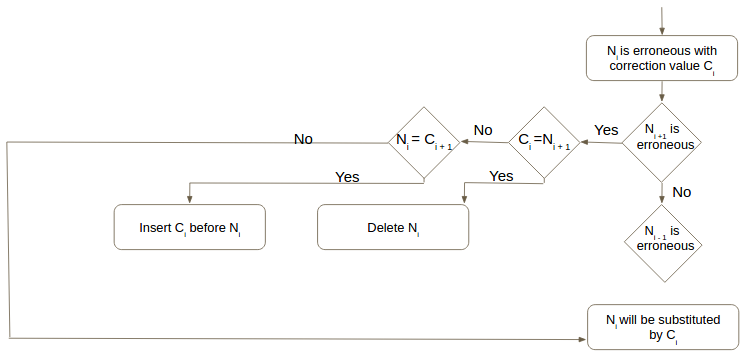
\includegraphics[width=1.3\linewidth]{./figs/Second-Proposal-1}
	\caption{\label{fig:fig-Second-Proposal-1}H-Racer Flow Chart}
\end{figure}


\begin{figure}
\vspace{0.2cm}
\begin{bordered}
\noindent\hspace{3ex}for every \textit{read} in \textit{reads} do

\noindent\hspace{6ex}for every \textit{nuc} in \textit{read} do

\noindent\hspace{9ex}if has\_error(\textit{nuc})

\noindent\hspace{12ex}if not\_last(\textit{nuc}) AND has\_error(next(\textit{nuc}))

\noindent\hspace{15ex}if correction(\textit{nuc}) equals to next(\textit{nuc})

\noindent\hspace{18ex}Delete \textit{nuc} from read

\noindent\hspace{15ex}else if \textit{nuc} equals to correction(next(\textit{nuc}))

\noindent\hspace{18ex}Insert correction(\textit{nuc}) before \textit{nuc} in read

\noindent\hspace{15ex}else 

\noindent\hspace{18ex}substitute \textit{nuc} with correction(\textit{nuc}) in read

\noindent\hspace{15ex}end if

\noindent\hspace{12ex}else if not\_first(\textit{nuc}) AND has\_error(previous(\textit{nuc}))

\noindent\hspace{15ex}if correction(\textit{nuc}) equals to previous(\textit{nuc})

\noindent\hspace{18ex}Delete \textit{nuc} from read

\noindent\hspace{15ex}else if \textit{nuc} equals to correction(previous(\textit{nuc}))

\noindent\hspace{18ex}Insert correction(\textit{nuc}) after \textit{nuc} in read

\noindent\hspace{15ex}else 

\noindent\hspace{18ex}substitute \textit{nuc} with correction(\textit{nuc}) in read

\noindent\hspace{15ex}end if		

\noindent\hspace{12ex}else 

\noindent\hspace{15ex}substitute \textit{nuc} with correction(\textit{nuc}) in read

\noindent\hspace{12ex}end if

\noindent\hspace{9ex}end if

\noindent\hspace{6ex}end for 

\noindent\hspace{3ex}end for 
\end{bordered}
\caption{\label{fig:fig-HRACER-PSC}H-RACER Pseudo-Code - O(\textit{r})}
\end{figure}
\newpage

\chapter{\label{chap:6}Experimental Results}
The evaluation chapter has two main sections. The first section illustrates the characteristics of the used datasets and how far they vary. While in the second section shows a discussion for the results of the comparison tests established between each of the proposed algorithms (KGEC and H-RACER) and the other existent algorithms in details.
\section{\label{sec:eval-data}Datasets and Platform}
The testing of both proposed algorithms was performed on a wide variety of real datasets, shown below in table \ref{tab:eval-data}, with different read length, genome size and coverage. It was preferred to use real datasets and to avoid any simulated ones as they do not offer a good indication of real life performance. 
\\
The testing datasets were selected to have variety in the lengths of the genome and the reads in addition to the number of reads and the reads coverage. ``Lactococcus Lactis" represents the smallest dataset in the running time, as its number of reads multiplied by its reads length shows the smallest number of nucleotides to be processed in comparison with the other datasets.
While ``Treponema Pallidum" represents the dataset with the highest coverage rate (hence the highest ambiguity), as its number of reads multiplied by its reads length divided by the genome length shows the highest value compared to the other datasets.
About ``E.coli 75a", it is a little bit larger dataset with the smallest coverage rate in comparison with other datasets. And finally, ``E.coli 75b" represents the largest dataset in the running time, as its number of reads multiplied by its reads length shows the smallest number of nucleotides to be processed in comparison with the other datasets.
\\
All datasets were brought from the National Center for Biotechnology Information (NCBI).
\\
All algorithms were executed on the same amazon elastic cloud (AWS EC2) instance with 32 vCPU and 244GiB RAM, with Linux (Ubuntu) operating system.

\begin{longtable}{|m{22mm}|m{21mm}|m{23mm}|m{16.5mm}|m{12mm}|m{17mm}|m{16mm}|}
	    \caption{\label{tab:eval-data}Datasets used in evaluation} \\
        \hline
        Name & Accession Number & Genome & Genome Length & Read Length & Number of Reads & Coverage\TBstrut\\ % top and bottom struts
        \hline
        Lactococcus Lactis & SRR088759 & NC\_013656.1 & 2,598,144 & 36 & 4,370,050 & 60.55\TBstrut\\ % top and bottom struts
        \hline
        Treponema Pallidum & SRR361468 & CP002376.1 & 1,139,417 & 35 & 7,133,663 & 219.13\TBstrut\\ % top and bottom struts
        \hline
        E.coli 75a & SRR396536 & NC\_000913.2 & 4,639,675 & 75 & 3,454,048 & 55.83\TBstrut\\ % top and bottom struts
        \hline
        E.coli 75b & SRR396532 & NC\_000913.2 & 4,639,675 & 75 & 4,341,061 & 70.17\TBstrut\\ % top and bottom struts
        \hline
\end{longtable}

\section{Results}
\subsection{\label{subsec:eval1-res}K-mer Grouping Error Correction Algorithm}
The comparisons, shown below in table \ref{tab:eval-0}, were established between K-mer Grouping Error Correction (KGEC) and the algorithms specialized in correcting all types of errors (substitutions, insertions, and deletions). While the obtained measurements were brought via the verification code implemented by RACER \cite{Racer}, that has the advantage of avoiding the interference of mapping or assembling programs. 
\\\\
For Lactococcus Lactis, the data with smallest size, the proposed algorithm shows the best accuracy with a very small difference (0.05\%), but with the worst time with a big difference; 1 hr compared to 15, 5, and 3 mins.
\\
\\
While for Treponema Pallidum, data with larger size, the algorithm has been running for more than 16 hrs compared to 22, 12, and 3 mins; which enforced the interruption of the running without getting the results.
\\
\\
For E.coli 75a and E.coli 75b, the largest dataset, the algorithm has been running for a day (24 hrs) without completion; which enforced the interruption of the running without getting the results.
\\
\\
The defect in time of this algorithm caused from the k-mers grouping steps illustrated above in chapter \ref{chap:4} specifically in section \ref{sec:alg1-meth}, where the algorithm is mainly dependent on the k-mers grouping, and the kmers grouping takes place by generating all of the possible cases of the corrections of every kmer, and here goes the time defect, as the complexity of the k-mers grouping step in exponential of the k-mers count.
\\
\\
The main major step of the proposal implies to its weakness point, which proves that this proposal will not get a better results, and in practice, some trials were done in order to replace the k-mers grouping and consequently the removal of the exponential complexity but it negatively affects the accuracy.

\begin{longtable}{|m{33mm}|m{20mm}|m{20mm}|m{20mm}|m{20mm}|}
	    \caption{\label{tab:eval-0}KGEC - Evaluation comparison table for Lactococcus Lactis}\\
        \hline
           & Coral & Pollux & HSHSREC & H-RACER\cellcolor{DarkGray} \TBstrut\\ % top and bottom struts
        \hline
           Accuracy & 91.45\% & 94.15\% & 95.34\% & 95.39\%\cellcolor{LightGray} \TBstrut\\ % top and bottom struts
        \hline
           Time in Minutes& 5 & 3 & 15 & 61\cellcolor{LightGray} \TBstrut\\ % top and bottom struts
        \hline
\end{longtable}


\subsection{\label{subsec:eval2-res}H-RACER Algorithm}
The comparisons, shown below in tables \ref{tab:eval-1}, \ref{tab:eval-2}, \ref{tab:eval-3}, and \ref{tab:eval-4}, were established between H-RACER and the algorithms specialized in correcting all types of errors (substitutions, insertions, and deletions). While the obtained measurements were brought via the verification code implemented by RACER \cite{Racer}, that has the advantage of avoiding the interference of mapping or assembling programs. 
\\\\
As shown below in the comparisons tables, H-RACER has the best results in accuracy and time. Actually, H-RACER aims to increase the genome reads accuracy, consequently, it aims to eliminate the errors existing in the genome reads. So, H-RACER avoided introducing errors to the reads by lowering the false positive rate and consequently increasing the specificity rate. On the other side, the false negative rate was negatively affected and the sensitivity rate was decreased as well. But, this approach did not negatively affect the accuracy, on contradictory, it resulted in getting the best accuracy.
\\
In other words, the high accuracy of H-RACER mainly resulted from both, the remarkable lowering of false positive rate and the high raising of true negative rate. On the other side, both, the true positive and false negative rates were negatively affected. Hence, H-RACER does not have neither the highest true positive nor the lowest false positive rates. And this is what H-RACER follows in RACER's footsteps, where it is preferred to lower the algorithm sensitivity represented in raising the false negative rate and lowering the true positive rate rather than raising the false positive rate and lowering the true negative rate. And this makes sense, as enhancing the reads overall accuracy is the main vital target. So, corrective algorithms should not introduce errors (represented in false positive rate), but it should target a higher gain to get higher accuracy, and so does RACER followed by H-RACER.
\\\\
The comparisons with the other algorithms, shown below in tables \ref{tab:eval-1}, \ref{tab:eval-2}, \ref{tab:eval-3}, and \ref{tab:eval-4}, prove that although the other algorithms have higher sensitivity than H-RACER, but all of them do not explicitly beat H-RACER accuracy, except for \enquote{Treponema Pallidum}, where HSHREC beats H-RACER's accuracy by 0.07\% and this is due to the high coverage rate of \enquote{Treponema Pallidum} that will be explained below.  
\\\\
For the short genome \enquote{Lactococcus Lactis}, illustrated in table \ref{tab:eval-1}, H-RACER shows the best results in specificity, gain, accuracy and time compared to CORAL, Pollux and HSHREC, although the sensitivity of H-RACER is not the best. But H-RACER gains the highest accuracy by lowering the false positive rate (as explained above).
\\\\ 
For \enquote{Treponema Pallidum}, the short genome with a very high coverage (the average number of reads representing a given nucleotide in the reconstructed sequence) as illustrated in tables \ref{tab:eval-data} and \ref{tab:eval-2}, H-RACER shows a lowering in the true positive rate with a raising in the false negative one rather than the expected rates. This is due to the very high coverage of \enquote{Treponema Pallidum} that increases the ambiguity for H-RACER in detecting the proper correction for some nucleotides, leading to a lowering in the true positive rate and consequently in the accuracy. But, by comparing such an accuracy with others, as illustrated in table \ref{tab:eval-2}, it is obvious that H-RACER shows the best results in specificity, gain, accuracy and time compared to CORAL and Pollux. While HSHREC is the only algorithm that beats H-RACER's gain and accuracy (for \enquote{Treponema Pallidum} only) with a very little difference rates (0.29\% and 0.07\% respectively). But, H-RACER accomplished such a correction in the best time compared to all others including HSHREC's (with a very remarkable ratio) and the best specificity as well.
\\\\
For long genomes \enquote{E.coli 75a} and \enquote{E.coli 75b}, illustrated in tables \ref{tab:eval-3} and \ref{tab:eval-4}, H-RACER obviously shows the best results in accuracy with a very perfect time, while CORAL and Pollux show lower accuracy with too much longer time, but HSHREC's running throws exception for such genomes, as SHREC (and consequently HSHREC) requires a very large space \cite{Racer}, \cite{HShrec}, so it is unable to run successfully for the larger genomes on the specified machine.
\\\\ 
Finally, the remarkable great difference in time between H-RACER and the rest of the algorithms is due to the bitwise orientation in implementation (inherited from RACER), and also H-RACER keeps RACER's complexity, consequently, H-RACER gains the advantage of having the best time. 
\newpage
\begin{longtable}{|m{33mm}|m{20mm}|m{20mm}|m{20mm}|m{20mm}|}
	    \caption{\label{tab:eval-1}H-RACER - Evaluation comparison table for Lactococcus Lactis}\\
        \hline
           & Coral & Pollux & HSHSREC & H-RACER\cellcolor{DarkGray} \TBstrut\\ % top and bottom struts
        \hline
           True Positive & 15,396,336 &  25,325,532 & 25,537,644 & 21,237,660\cellcolor{LightGray} \TBstrut\\ % top and bottom struts
        \hline
           False Positive & 2,039,148 &  7,720,920 & 6,053,580 & 19,656\cellcolor{LightGray} \TBstrut\\ % top and bottom struts
        \hline
           False Negative & 11,413,764 & 1,484,568 & 1,272,456 & 5,572,440\cellcolor{LightGray} \TBstrut\\ % top and bottom struts
        \hline
           True Negative & 128,472,552 & 122,790,780 & 124,458,120 & 130,492,044\cellcolor{LightGray} \TBstrut\\ % top and bottom struts
        \hline
           Sensitivity & 57.43\% & 94.46\% & 95.25\% & 79.22\%\cellcolor{LightGray} \TBstrut\\ % top and bottom struts
        \hline
           Specificity & 98.44\% & 94.08\% & 95.36\% & 99.98\%\cellcolor{LightGray} \TBstrut\\ % top and bottom struts
        \hline
           Gain & 49.82\% & 65.66\% & 72.67\% & 79.14\%\cellcolor{LightGray} \TBstrut\\ % top and bottom struts
        \hline
           Accuracy & 91.45\% & 94.15\% & 95.34\% & 96.45\%\cellcolor{LightGray} \TBstrut\\ % top and bottom struts
        \hline
           Time in Minutes& 5 & 3 & 15 & 1\cellcolor{LightGray} \TBstrut\\ % top and bottom struts
        \hline
\end{longtable}
\newpage
\begin{longtable}{|m{33mm}|m{20mm}|m{20mm}|m{20mm}|m{20mm}|}
	    \caption{\label{tab:eval-2}H-RACER - Evaluation comparison table for Treponema Pallidum}\\
        \hline
           & Coral & Pollux & HSHSREC & H-RACER\cellcolor{DarkGray} \TBstrut\\ % top and bottom struts
        \hline
           True Positive & 25,553,185 & 63,845,425 & 64,381,905 & 56,277,270\cellcolor{LightGray} \TBstrut\\ % top and bottom struts
        \hline
           False Positive & 3,462,165 & 8,832,320 & 8,133,895 & 223,405\cellcolor{LightGray} \TBstrut\\ % top and bottom struts
        \hline
           False Negative & 41,547,065 & 3,254,825 & 2,718,345 & 10,822,980\cellcolor{LightGray} \TBstrut\\ % top and bottom struts
        \hline
           True Negative & 179,115,790 & 173,745,635 & 174,444,060 & 182,354,550\cellcolor{LightGray} \TBstrut\\ % top and bottom struts
        \hline
           Sensitivity & 38.08\% & 95.15\% & 95.95\% & 83.87\%\cellcolor{LightGray} \TBstrut\\ % top and bottom struts
        \hline
           Specificity & 98.10\% &  95.16\% & 95.55\% & 99.88\%\cellcolor{LightGray} \TBstrut\\ % top and bottom struts
        \hline
           Gain & 32.92\% & 81.99\% & 83.83\% & 83.54\%\cellcolor{LightGray} \TBstrut\\ % top and bottom struts
        \hline
           Accuracy & 81.97\% & 95.16\% & 95.65\% & 95.58\%\cellcolor{LightGray} \TBstrut\\ % top and bottom struts
        \hline
           Time in Minutes& 12 & 3 & 22 & 2\cellcolor{LightGray} \TBstrut\\ % top and bottom struts
        \hline
\end{longtable}
\newpage
\begin{longtable}{|m{33mm}|m{20mm}|m{20mm}|m{20mm}|m{20mm}|}
	    \caption{\label{tab:eval-3}H-RACER - Evaluation comparison table for E.coli 75a}\\
        \hline
           & Coral & Pollux & HSHSREC & H-RACER\cellcolor{DarkGray} \TBstrut\\ % top and bottom struts
        \hline
           True Positive & 26,434,125 & 79,984,425 & N/A & 76,325,475\cellcolor{LightGray} \TBstrut\\ % top and bottom struts
        \hline
           False Positive & 5,549,925 & 31,675,650 & N/A & 33,000\cellcolor{LightGray} \TBstrut\\ % top and bottom struts
        \hline
           False Negative & 73,707,075 & 20,164,125 & N/A & 23,823,075\cellcolor{LightGray} \TBstrut\\ % top and bottom struts
        \hline
           True Negative & 153,362,475 & 127,229,400 & N/A & 158,872,050\cellcolor{LightGray} \TBstrut\\ % top and bottom struts
        \hline
           Sensitivity & 26.40\% & 79.87\% & N/A & 76.21\%\cellcolor{LightGray} \TBstrut\\ % top and bottom struts
        \hline
           Specificity & 96.51\% & 80.07\% & N/A & 99.98\%\cellcolor{LightGray} \TBstrut\\ % top and bottom struts
        \hline
           Gain & 20.85\% & 48.24\% & N/A & 76.18\%\cellcolor{LightGray} \TBstrut\\ % top and bottom struts
        \hline
           Accuracy & 69.40\% & 79.99\% & N/A & 90.79\%\cellcolor{LightGray} \TBstrut\\ % top and bottom struts
        \hline
           Time in Minutes& 9 & 16 & N/A & 1\cellcolor{LightGray} \TBstrut\\ % top and bottom struts
        \hline
\end{longtable}
\newpage
\begin{longtable}{|m{33mm}|m{20mm}|m{20mm}|m{20mm}|m{20mm}|}
        \caption{\label{tab:eval-4}H-RACER - Evaluation comparison table for E.coli 75b}\\
        \hline
           & Coral & Pollux & HSHSREC & H-RACER\cellcolor{DarkGray} \TBstrut\\ % top and bottom struts
        \hline
           True Positive & 13,312,725 & 99,375,600 & N/A & 81,059,700\cellcolor{LightGray} \TBstrut\\ % top and bottom struts
        \hline
           False Positive & 3,681,450 & 37,779,750 & N/A & 35,925\cellcolor{LightGray} \TBstrut\\ % top and bottom struts
        \hline
           False Negative & 108,494,025 & 22,439,925 & N/A & 40,755,825\cellcolor{LightGray} \TBstrut\\ % top and bottom struts
        \hline
           True Negative & 200,091,375 & 165,984,300 & N/A & 203,728,125\cellcolor{LightGray} \TBstrut\\ % top and bottom struts
        \hline
           Sensitivity & 10.93\% & 81.58\% & N/A & 66.54\%\cellcolor{LightGray} \TBstrut\\ % top and bottom struts
        \hline
           Specificity & 98.19\% & 81.46\% & N/A & 99.98\%\cellcolor{LightGray} \TBstrut\\ % top and bottom struts
        \hline
           Gain & 7.91\% & 50.56\% & N/A & 66.51\%\cellcolor{LightGray} \TBstrut\\ % top and bottom struts
        \hline
           Accuracy & 65.55\% & 81.50\% & N/A & 87.47\%\cellcolor{LightGray} \TBstrut\\ % top and bottom struts
        \hline
           Time in Minutes& 13 & 21 & N/A & 2\cellcolor{LightGray} \TBstrut\\ % top and bottom struts
        \hline
\end{longtable}

\newpage
\chapter{\label{chap:7}Conclusion and Future Work}
This chapter has two main sections, the conclusion and the future work. The conclusion section shows a very short briefed discussion about the proposed algorithms. While the future work section shows the major researchable points that can be investigated in the future.
\section{Conclusion}
The next-generation sequencing generated too many short reads in a reasonable time, but unfortunately it introduced too many errors with different type (substitution, insertion and deletion), and the accuracy of the reads decreased. But, accuracy of the output reads is a vital and a necessary factor, where the reads processes, applications and projects depends on it and  it is greatly affected by it. Consequently, fixing the errors and raising reads accuracy is an interesting field with many challenges.
\\
\\
The two proposed algorithms aim to fix all types of nucleotide errors (substitutions, insertions, and deletions) in a mixed set of reads, in order to raise the accuracy of the DNA sequencing output within the shortest time compared to the existent algorithms. 
\\
\\
K-mer Grouping Error Correction (KGEC - the first proposed algorithm) is mainly invented based on k-mers grouping and nucleotide frequencies and quality values. It accomplishes the correction mission properly with a high accuracy for the small dataset, but unfortunately it takes too much long time. Consequently, it is not able to compete for the larger dataset as it needs a very long time, which cannot be enhanced as this negatively effects the accuracy.
\\
\\
H-RACER (the second proposed algorithm) overcomes the time issue of the first algorithm and also it accomplishes the mission successfully, it is able to raise the next-generation sequencing output accuracy. 
\\
\\
H-RACER (the second proposed algorithm) comes up with the advantage of correcting different error types which were missed in RACER. H-RACER followed in the footsteps of RACER's implementation in order to acquire the major advantages of RACER in both aspects performance and time, then added its elegant algorithm in detecting the errors types and properly applying their corrections. Consequently, H-RACER shows great results in both performance and time compared to existent algorithms specialized in correcting all types of errors for large and small genome lengths. And by comparing H-RACER with existent algorithms specialized in correcting all types of errors, it is proved that H-RACER is the fastest with the highest accuracy algorithm.
\\
\\
Finally, both algorithms have been implemented in C/C++ as an open source program.
\\
\\
K-mer Grouping Error Correction (KGEC - the first algorithm) available at: 
\\
- github.com/salmagomaa/DNA-EC/tree/master/4-Best-49g-with-61(Best)
\\
\\
H-RACER (the second algorithm) available at: 
\\
- github.com/salmagomaa/H-RACER
\\
- drive.google.com/open?id=0B7Otgzz7lZlldkE2ZFVwcU5qN1U


\section{Future Work}
As a future work, the main target will be the memory usage enhancement for H-RACER specifically in long genomes, so as to be able to run long genomes within 244GiB RAM.
\\
\\
Also, one of the most interesting point to be added into consideration for the future work is implementing H-RACER with parallel threads, where both time and memory will be enhanced, especially for long genomes.
\\
\\
And finally, K-mer Grouping Error Correction (KGEC - the first proposed algorithm) can get another chance by inventing a new algorithm to group the k-mers in with a reasonable complexity instead of the exponential one.

\newpage

\clearpage\thispagestyle{empty}
% This is LLNCS.DOC the documentation file of
% the LaTeX2e class from Springer-Verlag
% for Lecture Notes in Computer Science, version 2.4
\documentclass[12pt,openany]{llncs}
\usepackage{llncsdoc}
\bibliographystyle{splncs}
%
% PACKAGES	
\usepackage[table]{xcolor}
\usepackage{csquotes}
\usepackage{mdframed}
\usepackage{float}
\usepackage{longtable}
\usepackage{graphicx}
\graphicspath{ {figures/} }
\usepackage{caption}
\usepackage{subcaption}
\usepackage[utf8]{inputenc}
\usepackage[LFE,LAE]{fontenc} 
\usepackage[arabic,english]{babel}
\usepackage{sectsty}

\allsectionsfont{\raggedright}

\captionsetup{compatibility=false}

%Cover page
\newcommand{\HRule}{\rule{\linewidth}{0.5mm}} % Defines a new command for the horizontal lines

\newmdenv[leftline=false,rightline=false,topline=false,bottomline=false,innertopmargin=2pt,innerbottommargin=2pt]{bordered}

% TABLE
\newcommand{\TBstrut}{{\rule{0pt}{7ex}}{\rule[2ex]{0pt}{0pt}}} % top&bottom struts
\definecolor{DarkGray}{gray}{0.6}
\definecolor{LightGray}{gray}{0.9}

\usepackage{tocloft}% http://ctan.org/pkg/tocloft
\setlength{\cftsubsecnumwidth}{4em}% Set length of number width in ToC for \subsection

\usepackage{titlesec}

\titleformat{\chapter}[display]
    {\normalfont\huge\bfseries}{\chaptertitlename\ \thechapter}{2pt}{\Huge}
\titlespacing*{\chapter}{0pt}{0pt}{4pt}

\makeatletter
\newcommand*{\centerfloat}{%
  \parindent \z@
  \leftskip \z@ \@plus 1fil \@minus \textwidth
  \rightskip\leftskip
  \parfillskip \z@skip}
\makeatother
%ABBREVIATIONS
\newcommand{\abbrlabel}[1]{\makebox[4cm][l]{\textbf{#1}\ \dotfill}}
\newenvironment{abbreviations}{\begin{list}{}{\renewcommand{\makelabel}{\abbrlabel}}}{\end{list}}

\begin{document}


\begin{titlepage}
{\small
\center % Center everything on the page

\includegraphics[scale=0.2]{./figs/aast}\\[0.7cm]
\selectlanguage{arabic}
{\large \bfseries 
الاكاديمية العربية للعلوم والتكنولوجيا والنقل البحرى
}\\[0.7cm]
{\large \bfseries 
كلية الحاسبات و تكنولوجيا المعلومات
}\\[1.3cm]
{\LARGE \bfseries 
خوارزميات لتصحيح الأخطاء الناتجة عن عملية تسلسل الحمض النووي
}\\[0.5cm]
{\large \bfseries 
إعداد
}\\[0.3cm]
{\large \bfseries
سلمى محمود محمد جمعة
}\\[0.3cm]
{\bfseries 
رسالة مقدمة للاكاديمية العربية للعلوم والتكنولوجيا والنقل البحرى
}\\[0.2cm]
{\bfseries
لاستكمال متطلبات درجة الماجستير
}\\[0.2cm]
{\bfseries
في
}\\[0.2cm]
{\large \bfseries
علوم الحاسب 
}\\[0.3cm]
{\large \bfseries 
إشراف
}\\[0.3cm]
\begin{minipage}{0.55\textwidth}
{\large \bfseries 
أ. د. ياسر علاء الدين السنباطى
}
\end{minipage}
~
\begin{minipage}{0.40\textwidth}
{\large \bfseries 
د. نهلة أحمد بلال
}
\end{minipage}
\\[0.1cm] 
\begin{minipage}{0.48\textwidth}
\begin{flushleft}
\center
{
أستاذ بكلية الحاسبات وتكنولوجيا المعلومات
}\\
{
الاكاديمية العربية للعلوم والتكنولوجيا والنقل البحرى
}
\end{flushleft}
\end{minipage}
~
\begin{minipage}{0.48\textwidth}
\begin{flushright}
\center
{
مدرس بكلية الحاسبات وتكنولوجيا المعلومات
}\\
{
الاكاديمية العربية للعلوم والتكنولوجيا والنقل البحرى
}
\end{flushright}
\end{minipage}\\[0.5cm]
{
 الاكاديمية العربية للعلوم والتكنولوجيا والنقل البحرى
}\\[0.1cm] 
{\bfseries
 7102
}\\[0cm]


\vfill % Fill the rest of the page with whitespace
}

\clearpage\thispagestyle{empty}

\selectlanguage{arabic}
\section*{ملخص}
إن عملية تسلسل الحمض النووي تعد من أكثر المجالات حيوية في علم الأحياء الحاسوبي. فإن معظم العمليات المرتبطة بالحمض النووي تعتمد في الأساس على عملية تسلسله؛ و من ثم أصبحت كلاً من تكلفة عملية التسلسل, و دقتها، و الوقت المستغرق فيها من العوامل الأساسية الهامة التي يقام عليها العديد من الأبحاث لتحسينها.
\\
\\
إن الهدف الأساسي للجيل الجديد من آليات تسلسل الحمض النووي هو تخفيض تكلفة عملية تحليل المحتوى الوراثي (الجينوم) الضخمة، و الإكثار من إنتشارها أيضاً؛ حيث إن تلك الآليات لديها القدرة على إنتاج العديد من القراءات القصيرة في وقت وجيز؛ و لكن من أهم الآثار الجانبية لتلك السرعة هي قصر طول القراءات مما أدى إلى وجود العديد من الأخطاء على مستوى النواة بأشكال مختلفة؛ مثل خطأ الناتج عن إبدال النواة، و الخطأ الناتج عن إدخال نواة جديدة، و أخيرا الخطأ الناتج عن حذف النواة. و تمثل كل هذه الأخطاء عقبة كبيرة تعوق إستخدام القراءات في المشاريع القائمة على التسلسل (مثل:  عملية تجميع القراءات، و عملية محاذاة المحتوى الوراثي (الجينوم)، إلخ)؛ لذلك أصبحت عملية تصحيح الأخطاء مهمة للغاية حيث إنها تعمل على تخفيض معدل الأخطاء على مستوى القراءات جميعاً؛ و من ثم أصبحت عملية تصحيح جميع أنواع الأخطاء أكثر تحدياً.
\\
\\ 
 تعد الخوارزميات المقدمة في تلك الرسالة من الآليات الجديدة التى تعمل على تصحيح جميع أنواع أخطاء التي تتعرض لها النواة (الإبدال، و الإدخال، و الحذف)؛ فكلتا الآليتين تعمل على زيادة الدقة الخاصة بناتج عملية تسلسل الحمض النووي في أقصر وقت ممكن مقارنة بالخوارزميات المجودة حالياً.
\\
\\
الخوارزم الأول يعتمد على إقامة مجموعات من نتاج تجزئة القراءات حيث يعتمد قرار التصحيح على تكرارات النوى. تلك الآلية قدمت دقة عالية لمجموعة البيانات الصغيرة؛ و لكنها عجزت عن إكمال مهمتها لتلك المجموعات الكبيرة؛ حيث إنها تحتاج لوقت طويل جداً ، بالإضافة إلى أن محاولة تحسين الوقت أثرت سلبياً على عامل الدقة.
\\
\\
 بينما تغلب الخوارزم الثاني على مشكلة الوقت التي أعاقت الخوارزم الأول بالإضافة أنه حقق الهدف الأساسي ألا و هو زيادة الدقة لناتج عملية تسلسل الحمض النووي. تلك الآلية تعتمد في إكتشاف الأخطاء و تقرير قيمة تصحيحه على الخوازم المسمى 
 \selectlanguage{english}RECAR 
 \selectlanguage{arabic}؛ حيث أن الميزة الرئيسية في تلك الآلية هي قدرتها على إكتشاف نوع الخطأ و من ثم تطبيق الإجراء التصحيحي المناسب. لذلك تلك الآلية لديها القدرة على تصحيح جميع أنواع الأخطاء بدقة عالية في أقصر وقت ممكن مقارنةً بالخوارزميات الموجودة حالياً المختصة بتصحيح جميع أنواع الأخطاء.

%%%%%END ABSTRACT

\clearpage\thispagestyle{empty}

\selectlanguage{english}
{
\center % Center everything on the page

\includegraphics[scale=0.2]{./figs/aast}\\[0.7cm]
{\Large \bfseries Arab Academy for Science, Technology and Maritime Transport \\[0.2cm](AAST)}\\[0.2cm]
{\large \bfseries College of Computing and Information Technology}\\[0.3cm]
{\large \bfseries Computer Science Department}\\[0.3cm] 
\HRule \\[0.2cm]
{\LARGE \bfseries DNA Sequencing Error Correction Algorithms}\\[0.1cm]
\HRule \\[0.2cm]
{\large \bfseries A Thesis}\\[0.2cm]
{\large \bfseries Submitted in Partial Fulfillment to the Requirements for the}\\[0.2cm]
{\Large \bfseries Master of Computer Science}\\[0.5cm]
{\large \bfseries Submitted by:}\\[0.2cm]
{\Large \bfseries Salma Mahmoud Mohamed Gomaa}\\[0.5cm]
{\large \bfseries Under Supervision of}\\[0.2cm]

\begin{minipage}{0.55\textwidth}
{\large \bfseries Prof.Dr.Yasser El-Sonbaty}
\end{minipage}
~
\begin{minipage}{0.40\textwidth}
{\large \bfseries Dr.Nahla A. Belal}
\end{minipage}\\[0.2cm]

\begin{minipage}{0.47\textwidth}
\begin{flushleft}
\center
{\small Professor of Computer Science}\\
{\small Arab Academy for Science, Technology, and Maritime Transport}
\end{flushleft}
\end{minipage}
~
\begin{minipage}{0.47\textwidth}
\begin{flushright}
\center
{\small Assistant Professor of Computer Science}\\
{\small Arab Academy for Science, Technology, and Maritime Transport}
\end{flushright}
\end{minipage}\\[0.2cm]
{\small June - 2017}\\[0cm] 
\vfill % Fill the rest of the page with whitespace
}
\clearpage\thispagestyle{empty}

\selectlanguage{english}
\section*{Abstract}
DNA sequencing is one of the very pivotal research fields in bioinformatics. Most of the processes that are related to the DNA genomes mainly depend on the DNA sequencing, and consequently the cost, the accuracy and the time of the DNA sequencing methodologies became very urgent and vital factors, that many researches are being done to enhance these critical factors.
\\
\\
The main targets of the next-generation sequencing technologies are: making the vast analysis of genomes less expensive and more spread, hence, they are able to produce large sets of short reads within a very efficient time. But, as a side effect of this fastness, the produced short reads are subject to be infected by different types of errors on the nucleotide level; such as nucleotide erroneous substitution, nucleotide erroneous insertion and nucleotide erroneous deletion. Since, these errors represent a great obstacle to utilize the reads in sequencing projects (such as: reads assemblers, genome aligners, etc.), the error correction process becomes a vital and essential action that aims to reduce the error rate over the whole reads set. So, the correction of all types of the nucleotides errors becomes very challenging.
\\
\\ 
The proposed algorithms are new error correcting tools that fix all types of nucleotide errors (substitutions, insertions, and deletions) in a mixed set of reads, where both of them aim to raise the accuracy of the DNA sequencing output, trying to accomplish the correction within a suitable time compared to the existent algorithms. 
\\
\\
K-mer Grouping Error Correction (KGEC - the first proposed algorithm) is mainly invented based on k-mers grouping and nucleotide frequencies. It shows a high accuracy for the small dataset but unfortunately it cannot compete for the larger dataset as it needs a very long time, which cannot be enhanced as this negatively effects the accuracy.
\\
\\
H-RACER (the second proposed algorithm) overcomes the time issue of the first algorithm using a large memory space and also it accomplishes the main target which is raising the sequencing output accuracy. It mainly depends on RACER algorithm in detecting the erroneous nucleotide and deciding its corrective value. While the major advantage presented by H-RACER is the detection of the nucleotide corrective action and applying it. So, H-RACER is able to correct the nucleotides substitutions errors as well as their insertions and deletions errors with the highest accuracy and the least time compared to other existent algorithms that specialize in correcting these types of nucleotides errors.

%%%%%END ABSTRACT
\end{titlepage}

\clearpage\thispagestyle{empty}
\section*{Acknowledgement}

I would like to seize this opportunity to express my sincere gratitude for the
unconditional and unlimited help and support that I have received from my supervisors Prof.
Dr. Yasser El-sonbaty and Dr. Nahla Belal. Their continuous guidance and tutoring were
critical for the successful completion of this thesis. Great part of the success of this research stems from the open access to the academy various facilities. 
\\
\\
All Gratitude is first due to ALLAH. Then, I'm deeply grateful for my father, my mother, my husband and my sisters for their enormous support in all aspects. Their continuous encouragement and motivation were the key for overcoming the obstacles encountered during the course of this research. I will be grateful forever for your love.
\\
\\
You all make the journey worthwhile .... Thank you all
\\
\\
\begin{flushright}
Salma Mahmoud Mohamed Gomaa\\
Computer Science, AASTMT,\\
June - 2017
\end{flushright}

\clearpage\thispagestyle{empty}
\section*{Published Work}
\noindent\hspace{0.6cm}The work in this thesis is published in one paper as follow:
\\
\\
Gomaa, S., Belal, N.A. and El-Sonbaty, Y.: H-RACER: Hybrid RACER to Correct Substitution, Insertion, and Deletion Errors. In International Conference on Bioinformatics and Biomedical Engineering (pp. 62-73). Springer, Cham (2017).

\newpage
\tableofcontents
\newpage
\listoffigures
\newpage
\listoftables
\newpage

{\Huge\bfseries List of Abbreviations}
\\
\begin{abbreviations}
\item[AWS EC2] Amazon Elastic Cloud
\item[Coral] Correction with Alignments
\item[CUDA] Compute Unified Device Architecture
\item[DNA] Deoxyribonucleic Acid
\item[EC] Error Corrector
\item[FN] False Negative
\item[FP] False Positive
\item[HiTEC] High Throughput Error Correction
\item[HSHREC] Hybrid Short Read Error Correction
\item[H-RACER] Hybrid RACER
\item[KGEC] K-mer Grouping Error Correction
\item[MSA] Multiple Sequence Alignments
\item[NGS] Next-generation Sequencing
\item[Pollux] Platform Independent Error Correction of 

\noindent\hspace{3.6cm}Single and Mixed Genomes
\item[Quake] Quality-aware Detection and Correction of 

\noindent\hspace{3.6cm}Sequencing Errors
\item[RACER] Rapid and Accurate Correction of Errors in 

\noindent\hspace{3.6cm}Reads
\item[Reptile] Representative Tiling for Short Read Error

\noindent\hspace{3.6cm}Correction
\item[TN] True Negative
\item[TP] True Positive
\end{abbreviations}

\chapter{\label{chap:1} Introduction}
This chapter gives a brief introduction to the thesis. It has three major sections, where it illustrates the problem statement, the thesis objective, and the thesis structure.
\\
\\
In bioinformatics, the DNA sequencing is one of the very pivotal research fields. Many researches has been done in order to enhance the DNA sequencing methodologies, as most of the processes that are related to the DNA genomes mainly depend on the DNA sequencing. So the cost, the accuracy and the time of the DNA sequencing methodologies became very urgent and vital factors, where the target of the researches is to enhance these critical factors.
\section{Problem Statement}
The next-generation sequencing (NGS) high-throughput technologies \cite{NGS} were originally proposed to make the vast analysis of genomes less expensive and more spread. So, their main target is the generation of too many reads in an efficient time. But unfortunately, this leads to negatively affecting the read length and the accuracy, where the read length becomes much shorter than the conventional sequencing, and the accuracy of the generated reads is decreased. 
\\
\\
In the generated reads, each erroneous nucleotide can be introduced to the read sequence via one of the three erroneous actions; which are substitution, insertion and deletion. 
The substitution erroneous action takes place when the nucleotide is substituted or replaced with another erroneous nucleotide. While the insertion erroneous action is the insertion or injection of a newly erroneous nucleotide into the read sequence. Finally, the deletion erroneous action results from the deletion or removal of a proper nucleotide from the read sequence.
\\
\\
The reads accuracy is a very vital factor, since, all of the processes, applications and projects that can be applied on the reads are affected by their accuracy. As an example, the assembly of next-generation sequencing (NGS) reads can not be accomplished successfully until the reads errors are corrected or eliminated. So detecting and correcting (or eliminating) the reads errors is an essential step that should precede the assembly process. 
\\
\\
In most of the error correction methodologies, the erroneous nucleotide detection and its correction value decision mainly depends on the nucleotide frequency with its quality value\cite{ErrCorr}. While, the error correction methodology itself can be accomplished either by a standalone solution or implicitly within the assembly mechanism. 

\section{Objective}
The newly proposed error correction methodologies aim to correct all types of errors (substitutions erroneous action, insertions erroneous action, and deletions erroneous action) in order to enhance the reads accuracy within a suitable time.
\\
Hence, the main objectives can be listed as:
\begin{itemize}
	\item Raising the DNA reads accuracy

	\item Correcting all of the different types of errors

	\item Accomplishing the correction process within the shortest time
\end{itemize}
The first algorithm has the ability to enhance the accuracy, but unfortunately it takes too much time to accomplish his mission. The analysis of the results and time of this proposal will be illustrated later in the following chapters. 
\\
While the second algorithm builds its correction decisions based on RACER \cite{Racer} (an already existent algorithm that handles substitution errors only and will be discussed in details later) with some tuning to handle the insertions and deletions errors. This algorithm has the ability to enhance both the accuracy and the time, as it shows almost the highest accuracy with the shortest time for different datasets in comparison with the existent algorithms specialized in correcting substitution, insertion and deletion errors.

\section{Thesis Structure}
This thesis documentation is organized as follows; illustrating some basics about deoxyribonucleic acid (DNA), deoxyribonucleic acid (DNA) sequencing, next-generation sequencing (NGS), and next-generation sequencing (NGS) errors correction in chapter \ref{chap:2}, while the  existing methodologies for error correction are demonstrated in chapter \ref{chap:3}, then the methodology of K-mer Grouping Error Correction (KGEC - the first proposed algorithm) is demonstrated in chapter \ref{chap:4}, while the methodology of H-RACER (the second proposed algorithm) is demonstrated in chapter \ref{chap:5}. In chapter \ref{chap:6}, the evaluation of both algorithms (K-mer Grouping Error Correction and H-RACER) are illustrated, where the comparisons set using experimental data. The conclusion and future work are shown in chapter \ref{chap:7}.
%

\newpage
\chapter{\label{chap:2}Background}
This chapter has five major sections, where it illustrates some basic information about deoxyribonucleic acid (DNA), DNA sequencing, next-generation sequencing (NGS) and NGS errors correction, in addition it shows the definition of the main concepts and terms used in NGS errors correction field.
\section{Deoxyribonucleic Acid}
Deoxyribonucleic Acid,or DNA  (Fig. \ref{fig:fig-DNA-1}), is the hereditary material in humans and almost all other organisms. Nearly every cell in an organism’s body has the same DNA. Most DNA is located in the cell nucleus (where it is called nuclear DNA) \cite{DNA1,DNA2}.
The information in DNA is stored as a code made up of four chemical bases: adenine (A), guanine (G), cytosine (C), and thymine (T). Human DNA consists of about 3 billion bases \cite{DNA4}, and more than 99 percent of those bases are the same in all people. The order, or sequence, of these bases determines the information available for building and maintaining an organism, similar to the way in which letters of the alphabet appear in a certain order to form words and sentences.
DNA bases pair up with each other, A with T and C with G, to form units called base pairs. Each base is also attached to a sugar molecule and a phosphate molecule. Together, a base, sugar, and phosphate are called a nucleotide. Nucleotides are arranged in two long strands that form a spiral called a double helix. The structure of the double helix is somewhat like a ladder, with the base pairs forming the ladder’s rungs and the sugar and phosphate molecules forming the vertical sidepieces of the ladder (illustrated in Fig. \ref{fig:fig-DNA-2}) \cite{DNA5}.
\newpage
\begin{figure}
	\centering
	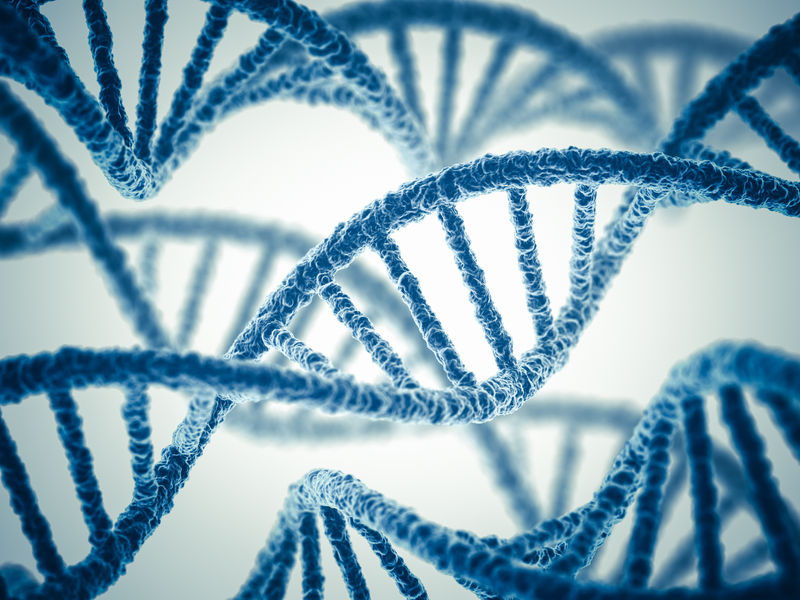
\includegraphics{./figs/DNA-1}
    \caption{\label{fig:fig-DNA-1}DNA}
\end{figure}

\begin{figure}
	\begin{subfigure}{.5\textwidth}
		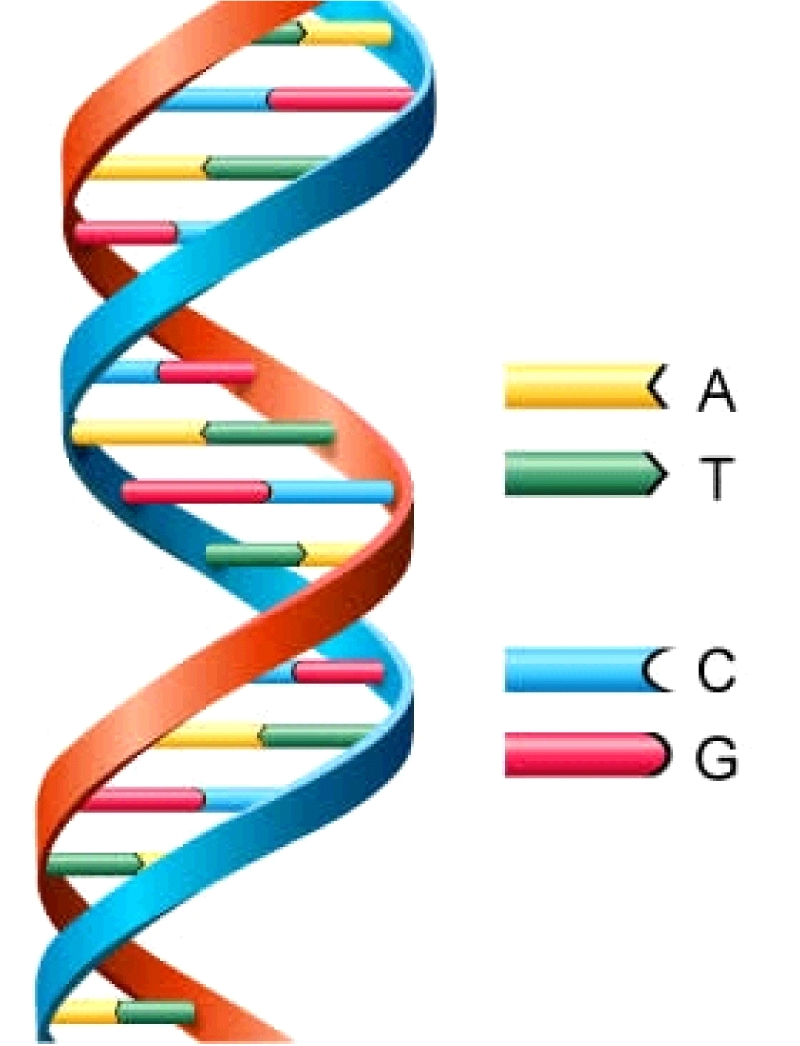
\includegraphics[width=.6\linewidth]{./figs/DNA-2}
	\end{subfigure}
	\begin{subfigure}{.5\textwidth}
		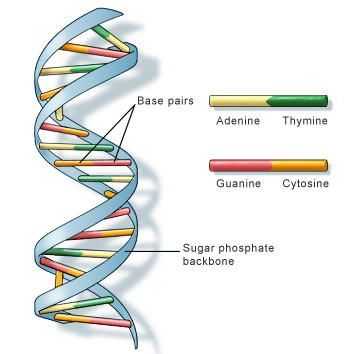
\includegraphics[width=.9\linewidth]{./figs/DNA-3}
	\end{subfigure}
	\caption{\label{fig:fig-DNA-2}DNA scientific analysis}
\end{figure}

An important property of DNA is that it can replicate, or make copies of itself. Each strand of DNA in the double helix can serve as a pattern for duplicating the sequence of bases. This is critical when cells divide because each new cell needs to have an exact copy of the DNA present in the old cell \cite{DNA3}.

\section{DNA Sequencing}
DNA sequence represents a single format onto which a broad range of biological phenomena can be projected for high-throughput data collection \cite{seq1}. 
Over the past years, massively parallel DNA sequencing platforms have become widely available, reducing the cost of DNA sequencing by over two orders of magnitude, and democratizing the field by putting the sequencing capacity of a major genome center in the hands of individual investigators. These new technologies are rapidly evolving, and near-term challenges include the development of robust protocols for generating sequencing libraries, building effective new approaches to data-analysis, and often a rethinking of experimental design (Fig. \ref{fig:fig-NGS-1} and \ref{fig:fig-NGS-2}) \cite{seq2,seq3}.
\begin{figure}
	\centering
	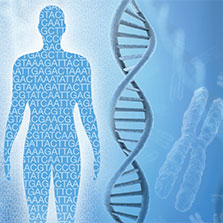
\includegraphics{./figs/NGS-1}
	\caption{\label{fig:fig-NGS-1}DNA sequencing}
\end{figure}

\begin{figure}
	\centerfloat
	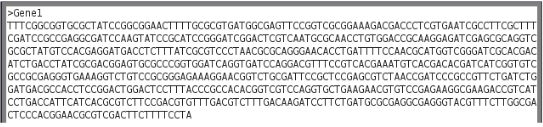
\includegraphics[width=1\linewidth]{./figs/NGS-2}
	\caption{\label{fig:fig-NGS-2}DNA sequencing - Gene example}
\end{figure}

\newpage
One of the core issues of Bioinformatics is dealing with file formats. Some ad hoc simple human readable formats have over time attained the status of de facto standards. A ubiquitous example of this is the ‘FASTA sequence file format’, originally invented by Bill Pearson as an input format for his FASTA suite of tools.
FASTA format is a text-based format for representing either nucleotide sequences, in which nucleotides are represented using single-letter codes. FASTA format allows for sequence names and comments to precede the sequences. As illustrated in Fig. \ref{fig:fig-NGS-5}, the first line in a FASTA file starts either with a ``\textgreater" (greater-than) symbol or, less frequently, a ``;" (semicolon) and was taken as a comment. Subsequent lines starting with a semicolon would be ignored by software. Since the only comment used was the first, it quickly became used to hold a summary description of the sequence, often starting with a unique library accession number, and with time it has become commonplace use to always use ``\textgreater" for the first line and to not use ``;" comments (which would otherwise be ignored) \cite{fasta-fastq1}.
\begin{figure}
	\centerfloat
	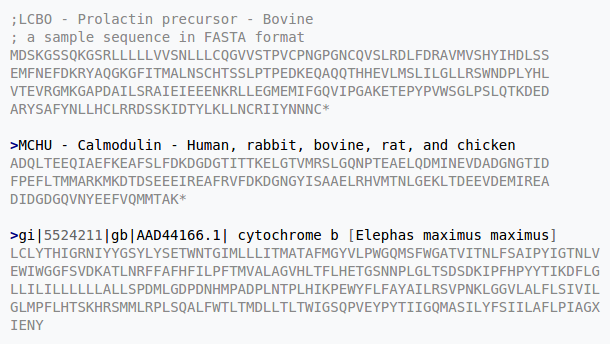
\includegraphics[width=0.8\linewidth]{./figs/NGS-5}
	\caption{\label{fig:fig-NGS-5}FASTA sample sequences}
\end{figure}
Following the initial line (used for a unique description of the sequence) is the actual sequence itself in standard one-letter code. Anything other than a valid code would be ignored (including spaces, tabulators, asterisks, etc...). Originally it was also common to end the sequence with an ``*" (asterisk) character. 
Over time, this format has evolved by consensus; however, in the absence of an explicit standard some parsers will fail to cope with very long ‘\textgreater’ title lines or very long sequences without line wrapping. There is also no standardization for record identifiers.

In the area of DNA sequencing, the FASTQ file format has emerged as another de facto common format for data exchange between tools. It provides a simple extension to the FASTA format: the ability to store a numeric quality score associated with each nucleotide in a sequence (illustrated in Fig. \ref{fig:fig-NGS-6}) \cite{fasta-fastq2}. 
Early FASTQ uses PHRED quality score \cite{fasta-fastq0} (which is a measure of the quality of the identification of the nucleobases generated by automated DNA sequencing where it is logarithmically linked to error probabilities as illustrated below in Fig. \ref{fig:fig-NGS-3} and \ref{fig:fig-NGS-4}). Storing PHRED scores as single characters (or bytes) gave a simple but reasonably space efficient encoding. In order that the file be human readable and easily edited, this restricted the choices to the ASCII printable characters 32–126 (decimal), and since ASCII 32 is the space character, ASCII 33–126 is used instead to encode PHRED qualities from 0 to 93 (i.e. PHRED scores with an ASCII offset of 33).

\begin{figure}
	\centerfloat
	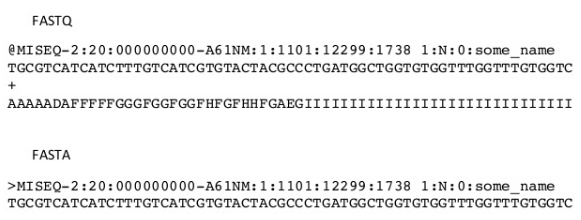
\includegraphics[width=0.9\linewidth]{./figs/NGS-6}
	\caption{\label{fig:fig-NGS-6}FASTQ VS FASTA}
\end{figure}

\begin{figure}
	\centering
	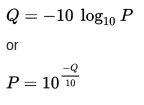
\includegraphics[width=0.4\linewidth]{./figs/NGS-3}
	\caption{\label{fig:fig-NGS-3}Phred quality scores 
	\textit{\textbf{Q}} are defined as a property which is logarithmically related to the base-calling error probabilities \textit{\textbf{P}}}
\end{figure}
\begin{figure}
	\centerfloat
	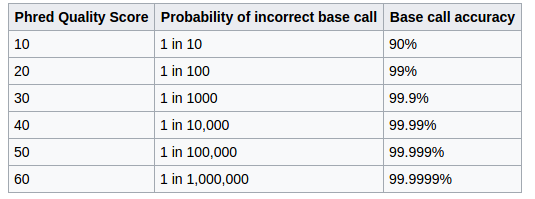
\includegraphics[width=1\linewidth]{./figs/NGS-4}
	\caption{\label{fig:fig-NGS-4}Phred quality scores are logarithmically linked to error probabilities}
\end{figure}


\section{Next-Generation Sequencing}
As stated above, the field of DNA sequencing technology development has a rich and diverse history. Over the past years, the incentive for developing entirely new strategies for DNA sequencing has emerged on at least four levels, undeniably reinvigorating this field\cite{NGS,NGS1}. First, in the wake of the Human Genome Project, there are few remaining avenues of optimization through which significant reductions in the cost of conventional DNA sequencing can be achieved. Second, the potential utility of short-read sequencing has been tremendously strengthened by the availability of whole genome assemblies for all major model organisms, as these effectively provide a reference against which short reads can be mapped. Third, a growing variety of molecular methods have been developed, whereby a broad range of biological phenomena can be assessed by high-throughput DNA sequencing. And fourth, general progress in technology across disparate fields, including microscopy, surface chemistry, nucleotide biochemistry, polymerase engineering, computation, data storage and others, have made alternative strategies for DNA sequencing increasingly practical to realize. Next-generation DNA sequencing has the potential to dramatically accelerate biological and biomedical research, by enabling the comprehensive analysis of genomes to become inexpensive, routine and widespread, rather than requiring significant production-scale efforts. Since the next-generation sequencing aims to make the vast analysis of genomes less expensive and more spread, it works on enhancing the sequencing time, where too many reads can be generated in a very efficient time. Consequently, it negatively affects the read length and also the sequences accuracy \cite{NGS2}. Actually the next-generation sequencing raises two critical issues, where the first issue is that the read length becomes much shorter than the conventional sequencing, while the second issue is the decrement of the accuracy, where each erroneous nucleotide can be introduced to the read sequence via any of the erroneous actions. There are three erroneous actions listed as; substitution, insertion and deletion illustrated in Fig. \ref{fig:fig-ErrCrr-1}, \ref{fig:fig-ErrCrr-2}, and \ref{fig:fig-ErrCrr-3} respectively. The substitution takes place when the nucleotide is replaced with another erroneous one, while the insertion is when an erroneous nucleotide is newly inserted to the read sequence, and finally the deletion results due to the deletion of a nucleotide from the sequence.

\begin{figure}
	\centerfloat
	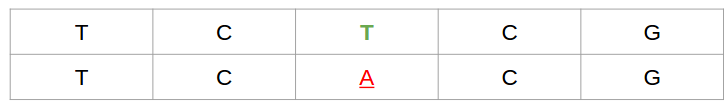
\includegraphics[width=1\linewidth]{./figs/ErrCrr-1}
	\caption{\label{fig:fig-ErrCrr-1}{Substitution Error} - \textbf{T} has been erroneously substituted with \underline{A}}
\end{figure}
\vspace{2cm}
\begin{figure}
	\centerfloat
	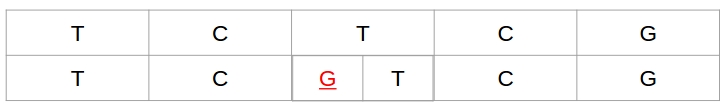
\includegraphics[width=1\linewidth]{./figs/ErrCrr-2}
	\caption{\label{fig:fig-ErrCrr-2}{Insertion Error} - \underline{G} has been erroneously inserted}
\end{figure}
\vspace{2cm}
\begin{figure}
	\centerfloat
	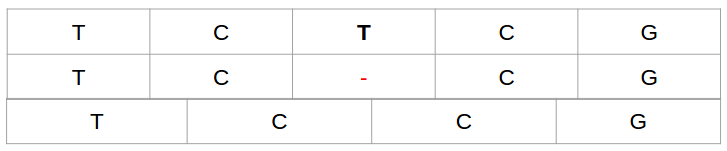
\includegraphics[width=1\linewidth]{./figs/ErrCrr-3}
	\caption{\label{fig:fig-ErrCrr-3}{Deletion Error} - \underline{T} has been erroneously deleted}
\end{figure}


\section{NGS Sequences Errors Correction}
The reads accuracy is a vital factor in all reads processes that can be applied to the output reads, like genome assemblers \cite{assembly,assembly1}, and genome aligners \cite{alignment}. For example, the assembly of next-generation sequencing reads can not be accomplished successfully until the reads errors are corrected or eliminated. So detecting and correcting (or eliminating) the reads errors is an essential step that should precede the assembly process. This step can be accomplished either by a standalone solution or implicitly within the assembly mechanism. The nucleotide frequency and its quality value are two main factors that are used in evaluating the nucleotide to erroneous or not \cite{ErrCorr,ErrCorr1}. 

\section{Correction Concepts and Definitions}
There are common concepts and definitions used by most of the corrective algorithms. Most of the corrective algorithms generates all the possible sub-sequences (of length k) from a read via a sliding window, which is called \textit{k-mer} (illustrated in Fig. \ref{fig:fig-CrrConcepts-1}); while the term k-mer frequency represents the number of repetition of a k-mer (a specific sub-sequence of length k) in all the reads. Some of the corrective algorithms set a threshold for the k-mer frequency while classifying the k-mer into strong and weak ones. The strong k-mers are those k-mers that are repeated all over the reads x times, where x is greater than the preset threshold; while the weak k-mers are those ones that are repeated y times all over the reads, where y is less than the k-mer frequency threshold. The filtration step that works on classifying the k-mers into strong and weak ones is called ``Spectrum Alignment". The spectrum alignment depends on the k-mers frequencies and/or the nucleotides quality values.
\\
A de Bruijn graph (illustrated in Fig. \ref{fig:fig-CrrConcepts-2}) can be constructed for any sequence, short or long. The first step is to choose a k-mer size, and split the original sequence into its k-mer components. Then a directed graph is constructed by connecting pairs of k-mers with overlaps between the first k-1 nucleotides and the last k-1 nucleotides. The direction of arrow goes from the k-mer, whose last k-1 nucleotides are overlapping, to the k-mer, whose first k-1 nucleotides are overlapping \cite{deBruijn,deBruijn1}.

\vspace{1cm}
\begin{figure}
	\centerfloat
	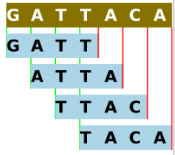
\includegraphics[width=.3\linewidth]{./figs/CrrConcepts-1}
	\caption{\label{fig:fig-CrrConcepts-1}{K-mer} - All the possible sub-sequences (of length k) from a read}
\end{figure}
\vspace{1cm}
\begin{figure}
	\centerfloat
	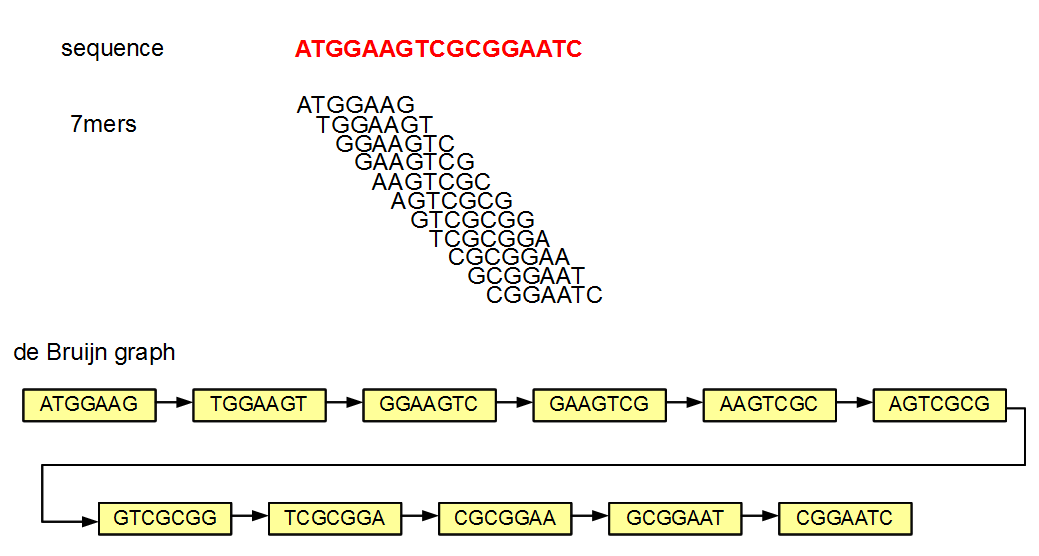
\includegraphics[width=1\linewidth]{./figs/CrrConcepts-2}
	\caption{\label{fig:fig-CrrConcepts-2}{De Bruijn Graph} - k-mer of length 7}
\end{figure} 
\newpage
\noindent The number of reads that include a given nucleotide in the sequence is called ``Coverage" \cite{coverage}. The coverage rate of a genome sequences is calculated by the following equation \ref{eq:coverage}
\begin{equation} \label{eq:coverage}
 C = L.N/G 
\end{equation}
where L is the average read length, N is the number of reads and G is the genome length.
\\
Some of the corrective algorithms uses the spectrum alignment in their correction decisions so that the correction takes place by obtaining the nucleotides substitutions that leads to reduce the weak k-mers count by converting them into strong k-mers.
In some other algorithms, the correction takes place using the tree breadth-first search by traversing multi out-going edges nodes, and removing the fewer reads paths, then re-aligning them to the existing path.
\\
There are some corrective algorithms that depend on the reads alignments, where the correction takes place by aligning reads with a common k-mer, then it fixes the misaligned nucleotides based on their occurrences and quality values.
The suffix array also is used in some of the corrective algorithms, where it is built using a string of reads, and the correction takes place with the letter that appears most at each position. Also the suffix trie is used in some other algorithms, where the edges are labelled with DNA letters, while the correction is based on the number of leaves in the sub-trie rooted at the node.
\\
The k-mer hashing table is also used in some corrective algorithms, it is used in storing the total times each nucleotide appears before and after a k-mer, where the error is corrected via the counts. 
\\
Also the k-mer discontinuities is used in some algorithms where the frequencies of adjacent k-mers are calculated and the correction is based on the removal or minimizing the discontinuity.
All of the concepts, stated above, represent the major concepts and paradigms used in the algorithms specialized in correcting the DNA sequencing errors.
\\
The accuracy evaluation of the corrective algorithms depends on calculating some factors as, the true positive rate, the false positive rate, the false negative rate, and the true negative rate. The true positive rate (TP) is the count of the properly corrected nucleotides, while the false positive rate (FP) is the count of the non-erroneous nucleotides that have been wrongly corrected. The false negative rate (FN) is the count of the erroneous nucleotides that haven't been detected as erroneous by the algorithm, while the true negative rate (TN) is the count of the non-erroneous nucleotides that have been properly detected as non-erroneous ones. These four factors are the basics factors that are used in calculating the specificity, sensitivity and the accuracy of the algorithm \cite{analysis}. The specificity rate represents the ability of the algorithm to properly corrects the erroneous nucleotides, and it is calculated by the following equation \ref{eq:sensitivity}:
\begin{equation} \label{eq:sensitivity}
  Sensitivity = TP/(TP+FN) 
\end{equation}
While the sensitivity rate represents its ability to detect the erroneous nucleotides, and it is calculated by the following equation \ref{eq:specificity}: 
\begin{equation} \label{eq:specificity}
  Specificity = TN/(TN+FP) 
\end{equation}
And finally, the accuracy represents the all over error rate, and it is calculated by the following equation \ref{eq:accuracy}:
\begin{equation} \label{eq:accuracy}
  Accuracy = (TP+TN)/(TP+FP+FN+TN)
\end{equation} 
While the gain represents the percentage of errors removed from the data set by the error correction program, and it is calculated by the following equation \ref{eq:gain}:
\begin{equation} \label{eq:gain}
  Gain = (TP-FP)/(TP+FN)
\end{equation} 



\newpage
\chapter{\label{chap:3}Related Work}
This chapter has two major sections, where it shows the different types of NGS errors correction algorithms, and briefly gives an overview for every existent error correction algorithm.
\\
\\
The error correction methodologies can be either an implicit process within the assembly methodology or a standalone solution that reproduces reads after correction. The assemblers that have embedded error correction are Euler \cite{Euler}, Velvet \cite{Velvet}, AllPaths \cite{AllPaths} and SOAP \cite{Soap}. While the standalone methodologies are Coral \cite{Coral}, Quake \cite{Quake}, Reptile \cite{Reptile}, HSHREC \cite{HShrec}, HiTEC \cite{HiTec}, RACER \cite{Racer}, Pollux \cite{Pollux}, Parallel Error Correction with CUDA \cite{Cuda}, and Error Corrector (EC) \cite{EC}.
\section{Substitution Only Corrective Algorithms}
They are algorithms that are able to correct only the substitution DNA reads errors, these algorithms are: Euler \cite{Euler}, Velvet \cite{Velvet}, AllPaths \cite{AllPaths}, SOAP \cite{Soap}, Quake \cite{Quake}, Reptile \cite{Reptile}, HiTEC \cite{HiTec}, RACER \cite{Racer}, Parallel Error Correction with CUDA \cite{Cuda}, and Error Corrector (EC) \cite{EC}. Check Fig. \ref{fig:fig-RW-1}.
\subsection{Euler}
Euler \cite{Euler} assembly method runs a filtration step called spectrum alignment that aims to classify the k-mers into two categories according to their frequencies all over the reads. Strong k-mers are the ones with high frequencies, while weak k-mers are the ones with lower frequencies. The correction takes place by executing a greedy exploration for base call substitutions aiming to reduce the weak k-mers count.
\\
Since in de novo genome sequencing the sampled genome is not known, EULER uses the number of times a k-mer appears to determine if it is in Gk(the set of k-mers in a genome G), where a threshold M determines whether a k-mer is a solid or a weak one. The read that contains all solid k-mers is referred to as a solid read. Hence, the goal of EULER is to correct the reads so that they are all solid reads.
\\
And the set of all k-mers is updated after each iteration of corrections, so that the reads are deleted if they are not able to be corrected after the last iteration. After that, the assembly of the genome begins after the error correction.
\\
The datasets with low coverage require that the threshold M to be set with a low value so that valid k-mers are not considered weak, but this will cause correct reads to be considered incorrect. 
Where increasing the length of k, will help in reducing the false positive rate and increasing the difficulty of determining the correction changes.
\\
Also in Euler, the reads with erroneous ends are trimmed, because the ends of reads tend to have more errors than the rest of the read, so it's difficult to determine the correct changes to the ends of reads.

\subsection{Velvet}
Velvet's \cite{Velvet} works by efficiently manipulating de Bruijn graphs through simplification and compression, without the loss of graph information, by converging non-intersecting paths into single nodes, i.e. it merges nodes that do not affect the path generated in the graph, so that, whenever a node A has only one outgoing arc that points to node B, with only one ingoing arc, the nodes can be merged.
\\
Velvet eliminates errors and resolves repeats by first using an error correction algorithm that merges sequences together. Repeats are then removed from the sequence via the repeat solver that separates paths which share local overlaps.
\\
\\
In other words, velvet's tour bus algorithm uses breadth-first search (BFS), starting at nodes with multiple out-going edges, where candidate paths are traversed in step, moving ahead one node on all paths per iteration, until the path lengths exceed a threshold. Velvet removes the path representing fewer reads then re-aligns reads from the removed path to the remaining path.

\subsection{AllPaths}
AllPaths \cite{AllPaths} uses a read-correcting preprocessor related to the spectral alignment in Euler, where the reads filtration is based on quality values, which is further used in correcting some substitutional errors. 

\subsection{SOAP}
SOAP \cite{Soap} filters and corrects reads using pre-set thresholds for k-mer frequencies. It removes bubbles with an algorithm like Velvet's tour bus, with higher read coverage determining the surviving path (read).

\subsection{Quake}
Quality-aware Detection and Correction of Sequencing Errors (Quake) \cite{Quake} determines a cut-off value which separates trusted k-mers from untrusted k-mers, using the distribution of k-mers based on their quality scores. The intersection of the untrusted k-mers is used to localize the search for an error in a read. Quake tries to evaluate the conditional probability of assigning the actual nucleotides of the sequenced fragment, given the observed nucleotides.
\\
It relies on k-mer coverage and quality scores to correct reads, as it uses a method of evaluating the quality of a k-mer based on the associated quality scores for each base. 
\\
The k-mers weighing is based on quality scores, where the low coverage true k-mers will have high quality scores and the high coverage k-mers with errors will have low quality scores.
\\
Quake begins by counting all the k-mers in the dataset, so the value of k, has a significant impact on the performance of Quake. But actually for an appropriate choice for k, Quake uses the following equation \ref{eq:quake-k} to set k (where G is the size of the genome).
\begin{equation} \label{eq:quake-k}
 k \approx log_{4} 200G  
\end{equation}
After that, it determines a cut-off value which separates trusted k-mers from untrusted k-mers, using the distribution of k-mers based on their quality values, where the reads with untrusted k-mers are considered for correction, and the errors are detected based on the intersection of the untrusted k-mers, which is used to localize the search for an error in a read. 
\\
Actually, Quake considers every base covered by the right most trusted k-mer, and left most trusted k-mers to be correct, so if the errors are near the end of a read, it will be checked first whether it is in the right most or left most, after that the decision will be taken. Also it tries to evaluate the conditional probability of a assigning the actual nucleotides of the sequenced fragment, given the observed nucleotides.
\\
\\
Quake has some heuristics, like ambiguous true correction, where the repeats imply to having multiple sets of valid corrections, with a small difference in the likelihood of each correction, so a true correction is ambiguous. So, it continues past the threshold to ensure that another valid set does not exist. 
\\
Quake stops correcting if the region is filled with low quality scores, where the reads with a region containing $\geq$ 13 positions with a probability of error $>$ 1\% are not corrected. And the reads with regions containing $\geq$ 9 positions with a probability of error $>$ 1\%, the likelihood ratio threshold is increased to $10^{-3}$.
\subsection{Reptile}
Representative Tiling for Short Read Error Correction (Reptile) \cite{Reptile} uses the spectral alignment approach used in Euler, with the quality score information if available. Trying to create approximate multiple alignments by considering all reads with pairwise hamming distance less than a pre-set threshold. 
\\
\\
Reptile considers all reads with pairwise Hamming distance less than a set threshold, where it finds the multiple alignments by only aligning k-mers in the reads. Actually, it chooses the size of k so that the expected number of occurrences of any k-mer in the genome should not exceed one. And it uses contextual information to help resolve errors without increasing k.
\\
\\
The main disadvantage of Reptile is that the user should set the parameters, so it
requires running scripts and analyzing the results to obtain the proper parameters.

\subsection{HiTEC}
High Throughput Error Correction (HiTEC) \cite{HiTec} uses a suffix array that is built using a string of reads and their reverse complements. The correction of an erroneous nucleotide takes place with the letter that appears most at that position.
\\
\\
HiTec uses the suffix array as it is a more time and space efficient data structure than the suffix trie, where it uses an array that stores the length of the longest common prefix (LCP) between consecutive suffixes in the suffix array.
\\
\\
Actually, it assumes that the length of the genome and the error rate of the dataset is supplied. Also HiTEC assumes that a read, starting at position j of the genome, contains an error in position m and that the previous w positions, $r_{i} [m - w..m - 1]$, are correct.
\\
As the length of witness length (w) decreases:

\begin{itemize}
	\item The number of uncorrectable reads U(w) decreases.
	\item The probability of seeing the witness increases, so the correct positions changed incorrectly. 
	\item The number of destructible reads D(w) increases.
	\item A value for w must be found that minimizes U(w)+ D(w). 
\end{itemize}

So, HiTEC uses a variation of witness lengths based on the optimal witness length to achieve high accuracy.
\\
\\
After that, HiTEC uses the majority of one base at a position, the erroneous base is changed to the base that appears most at that position. If there is no ambiguity in the correct letter then the correction is made. But, if there is ambiguity, then the next two letters are checked in order to decide how to correct the read. And finally, it stops correcting when the number of bases changed during one iteration is less than 0.01\% of the total number of bases, or after nine iterations or corrections.
\\
\\
HiTEC only requires modest coverage to make corrections. So, the datasets with high coverage are split into several sets with lower coverage that are independently corrected. 
\\
\\
The disadvantages of HiTEC can be listed as:
\begin{itemize}
	\item It does not correct reads with ambiguous letters.
	\item It can only correct datasets if the reads are all the same length.
	\item It does not run in parallel mode.
\end{itemize}

\subsection{RACER}
Rapid and Accurate Correction of Errors in Reads (RACER) \cite{Racer} is able to correct datasets that have varying read lengths. Using a hash table that stores the total number of times each nucleotide appears before and after each k-mer, where the error is corrected via the counts.
\\
\\
Actually, RACER replaces the suffix array approached used in HiTEC with a more time and space efficient hash table. And as stated above, this hash table stores the k-mers in each read, and the total times each base appears before and after each k-mer. While, the optimal k-mer length is calculated with a similar statistical analysis as HiTEC, i.e, it's value must be found that minimizes U + D, where U is the number of uncorrectable reads and D is the number of destructible reads. In other words, it choose k that will minimize the number of false positives and maximize the number of corrections. And after the k-mers and the counters have been calculated, the reads are corrected based on the counts.
\\
\\
RACER encodes the input sequences using two bits to represent each base, where the k-mer and its reverse complement must be searched, and only the one with the smaller encoding key is stored. Consequently, it shows a great enhancement in time and memory usage, where there is no algorithm can beat RACER in time.
\\
One more significant advantage of RACER is that it is able to correct datasets that have varying read lengths, and runs in both serial and parallel mode.
 

\subsection{Parallel Error Correction with CUDA}
Parallel Error Correction with Compute Unified Device Architecture (CUDA) \cite{Cuda} uses the spectrum alignment besides a voting algorithm for the single-mutation using each letter, hence errors can be fixed based on high values in the voting matrix.
\\
\\
CUDA (Compute Unified Device Architecture) is an extension of C/C++ to write scalable multi-threaded programs for CUDA-enabled GPUs, where CUDA programs can be executed on GPUs with NVIDIA’s Tesla unified computing architecture, while CUDA programs contain a sequential part, called a kernel.
\\
\\
CUDA uses the single-mutation voting algorithm, where it firstly initialize the voting matrix by zeros for each of (A, C, T, G) for every nucleotide, and loop on every read to check whether it is in the spectrum or not. If it is found that the read is not in the spectrum, it loops on every nucleotide against its voting matrix and increase the vote by 1 for every successful replacement (that makes the reads fit into the spectrum). After that, the errors can be fixed based on high values in the voting matrix.
\subsection{Error Corrector}
Error Corrector (EC) \cite{EC} an error correction algorithm for correcting short reads with substitution errors only. Using k-mers hashing tables to find the neighbours of each of the reads, where each read is corrected using its neighbours.
\\
\\
In other words, the steps of Error Corrector (EC) can be broken into three independent tasks. At first it builds k-mers and hashes the k-mers into hash tables. After that, by using these hash tables it finds the neighbours of each of the reads. And finally, each read is then corrected using the neighbours of the read.

\begin{figure}
	\centerfloat
	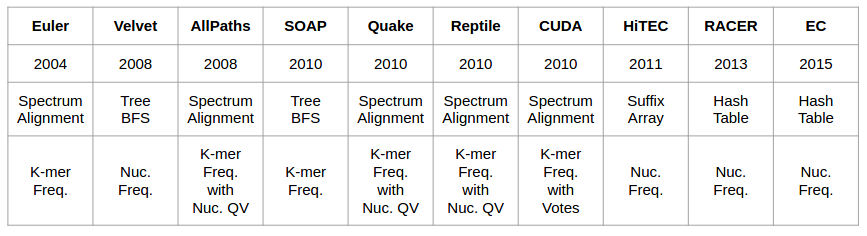
\includegraphics[width=1.35\linewidth]{./figs/RW-1}
	\caption{\label{fig:fig-RW-1}An illustrative summary for the substitution only corrective algorithms}
\end{figure}


\section{Substitution, Insertion And Deletion Corrective Algorithms}
They are algorithms that are able to correct all types of DNA reads errors, these algorithms are: Coral \cite{Coral}, HSHREC \cite{HShrec}, and Pollux \cite{Pollux}. Check Fig. \ref{fig:fig-RW-2}

\subsection{Coral}
Correction with Alignments (Coral) \cite{Coral} is able to correct all types of errors (substitution, insertion and deletion). The methodology is built on scoring the alignments between short reads, where each alignment runs on a base read with all the reads that have at least one common k-mer with this base read. Then the correction takes place for the misaligned positions depending on the number of times each letter occurs in addition to quality scores of the nucleotide.
\\
Coral uses multiple sequence alignments (MSA) \cite{coral-alignment} between short reads to detect errors, where it calculates the gap penalty and mismatch penalty (parameters for scoring the alignments) have a significant impact on the quality of the corrections. 
\\
The main defect in Coral is that it isn't able to correct mixed datasets that contain both substitution errors with insertion and deletions ones.
For substitution errors, Coral sets the gap penalty with a very high value to prevent insertions and deletions in the alignments. While for insertion and deletion errors, Coral sets the gap and mismatch penalties to be equal.
\\
Coral can summarize the algorithm as:
\begin{enumerate}
	\item Indexing Reads, where a hash table is used to store the k-mers and the reads that contain each k-mer. And in order to save space, Coral store the information of only the lexicographically smaller of the k-mer \& its reverse. It also does not store any k-mers that contain ambiguous letters.
	\item Multiple Alignments, where Coral starts each alignment with one read which is called the base read, and all the reads that share at least one k-mer with the base read are found using the k-mer hash table, and they are called neighbourhood of the base. If the neighbourhood of the base read is very large or very small, then Coral does not perform any alignments.
 As, if it's very large, then the reads likely came from different regions in the genome and the MSA will take a long time to compute, as the alignments will be very poor. But, if it's very small, then there is likely not enough coverage to make any significant corrections.
\\
Coral doesn't correct the reads that have been corrected before. So, if a read has already been corrected in a previous alignment, Coral tries to align it to the consensus without errors in the region of the k-mer. And, if a read aligns perfectly to the consensus then the rest of the read is not aligned to save time. But, if a read has many errors compared to the consensus then it stops aligning the read and moves on to the next one. And if the gaps are not allowed then a gap-less alignment is performed between a read and the consensus sequence.

\item Correcting Reads, where Coral calculates the number of misaligned positions for each read compared to the consensus sequence. And if the quality of the alignment is above a preset threshold, then it will be used to correct the aligned reads. The support threshold for each position in the consensus sequence is calculated as: (num of times each letter occurs)/ (total num of reads aligned at that position). In case a read differs from the consensus at any position, then the letter is changed in the read provided the support is above the threshold. And if quality scores are available and there is a gap in an aligned read, then:
 quality score of the gap = avg (the quality scores of the bases flanking the gap).
\end{enumerate}
The complexity of Coral is illustrated as follow (assuming that where M is the combined total length of the reads, L is the maximum number of reads in a neighbourhood, and r is the longest read length):
\begin{itemize}
	\item If gaps are allowed, the worst case runtime is O(MrL).
	\item If only mismatches are allowed, the worst case runtime is O(ML).
	\item The space for the hash table that stores the k-mers is bounded by O(M).
	\item The space complexity for computing the MSA is O(Lr + r\textsuperscript{2}).
	\item The overall space complexity is O(M).
\end{itemize}

\subsection{HSHREC}
Hybrid Short Read Error Correction (HSHREC) \cite{HShrec} is able to correct all types of errors (substitution, insertion and deletion). The methodology depends on the alignment of a read with others using a suffix trie, where the edges are labelled with DNA letters and a node weight is the number of leaves in the sub-trie rooted at that node. On the down levels, a node with more than one child is considered to have a substitution error, while extra branching in the generalized suffix trie is caused by insertion and deletion erroneous actions.
\\
\\
SHREC was designed to correct substitution errors, and HSHREC is able to correct both substitution errors and insertion and deletion erroneous actions.
\\
HSHREC assumes that the input contains k reads randomly sampled from a genome with read length n, where n can vary in length. The errors are detected in a read by aligning it to the other reads using a suffix trie, where the erroneous region of the read has a low weight in the trie and this is the area that will be corrected.
\\
\\
HSHREC resolves the ambiguity that can be caused by single nucleotide polymorphisms (SNPs). The single nucleotide polymorphisms (SNPs) is the phenomena of changing single nucleotide that differ between individuals of the same species, and they can appear as errors. Actually, SNPs are the most abundant type of genetic marker and their high density makes them ideal for studying the inheritance of genomic regions \cite{SNP1,SNP2}, so its discovery and genotyping are essential to genetic mapping. There remains a need for a simple, inexpensive platform that allows high-density SNP discovery and genotyping in large populations \cite{SNP3}. But HSHREC analyse it as: since the errors at the SNP location will only be in a few reads, and SNPs will be present in several reads, it is possible to differentiate them.
\\
\\
In HSREC, each read has a unique suffix by concatenating a unique number from 1 to 2k to the end of each string in R (the set of reads, and their reverse complements). And the edges of the trie are labeled with DNA letters, and an ambiguous letter N, where the concatenation of edge labels from the root to a node is called a path-label. 
\\
For any suffix of a string in R, there is a path-label that contains that suffix. And the weight of a node in the trie is the number of leaves in the subtrie that is rooted at that node, and is the number of suffixes in that subtrie. 
\\
The level of a node is the length of the path from the root to the node. In the top levels of the trie almost all nodes have four or five children. while in the down levels of the trie almost all nodes have only one child. So, if a child at down levels has more than one child then it is likely an error, and the node with the lower weight is likely the erroneous base. 
\\
So, HSHREC algorithm traverses the trie to identify errors at the intermediate levels of the trie. And it tries to correct each error with a substitution, and the remaining errors are treated as insertions or deletions.
\\
In SHREC, it compares the subtrie rooted at the low weight node to the subtries rooted at the siblings of the node, while the insertion and deletion erroneous actions cause extra branching in the generalized suffix trie. The insertion erroneous action creates a low weight node, so the deletion corrective action of the node causes the children rooted at the node and their siblings to be merged. And a comparison of the subtries before and after the deletion determine if the deletion is a proper way to correct the node or not. 

\subsection{Pollux}
Platform Independent Error Correction of Single and Mixed Genomes (Pollux) \cite{Pollux} calculates the k-mer frequencies in the entire set of reads. Identifying the discontinuities by comparing the frequencies of adjacent k-mers within reads, assuming that individual k-mers are not erroneous. The discontinuities within reads are used to find error locations and evaluate correctness. The correction is chosen to be the one that removes or minimizes the k-mer count discontinuity.
\\
\\
Pollux decomposes each read into k-mers and then calculates the k-mer frequencies in the entire set of reads. The nucleotide is represented with a two-bit alphabet and a hash-table strategy is used to help in using large k-mers (with length 31) to avoid common short repeats which might otherwise confound the correction procedure.
\\
\\
Firstly it identifies the individual k-mers as not erroneous, then identifies the discontinuities by comparing the frequencies of adjacent k-mers within reads. The discontinuities within reads are used to find error locations and evaluate correctness. A read that is not erroneous is assumed to have a k-mer count profile that is reflective of a random sampling process, given local coverage. In contrast, a read that contains an error is likely to have k-mer counts that deviate unexpectedly from this random process. Evaluating multiple k-mers containing bases following the erroneous base to ensure our correction is appropriate. The correction is chosen to be the one that removes or minimizes the k-mer count discontinuity. If there exist multiple corrections which achieve this, the correction is chosen to be the one that improves the most k-mer counts maximally beyond the current erroneous location. Pollux corrects each read independently and does not update recorded k-mer counts as a result of correction.
 
\begin{figure}
	\centerfloat
	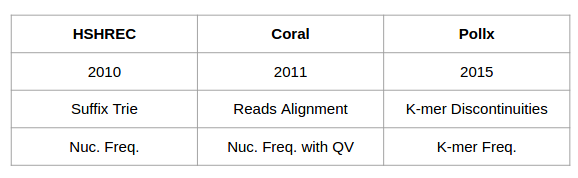
\includegraphics[width=1.35\linewidth]{./figs/RW-2}
	\caption{\label{fig:fig-RW-2}An illustrative summary for the substitution, insertion and deletion corrective algorithms}
\end{figure}

\newpage
\chapter{\label{chap:4}K-mer Grouping Error Correction Algorithm}
This chapter illustrates the working methodology of K-mer Grouping Error Correction (KGEC - the first proposed algorithm) in details, where the pseudo code, diagram and examples are discussed in details. While the evaluation will be discussed in chapter \ref{chap:6}.
\\
\\
The first proposed algorithm (Kmer Grouping for Error Correction or KGEC) aims to correct all types of errors and to boost the next-generation sequencing output accuracy. It tries to compete in the accomplishment time with the currently existent algorithms specialized in correcting all types of the errors found in the output of the next-generation sequencing, i.e. the substitution erroneous actions, the insertion erroneous actions and the deletion erroneous actions). Also it has the flexibility to run more than a correction iteration, which usually helps in enhancing the accuracy.
\section{\label{sec:alg1-meth}Methodology}
As stated before, this algorithm aims to correct all types of errors (substitution, insertion and deletion). It mainly depends on k-mers grouping. So, firstly it builds a hash table that maps the k-mer into integer and saves its frequency all over the reads. The hashing algorithm (illustrated in Fig. \ref{fig:fig-KGEC-HASH}) is inherited from Coral \cite{Coral}, where the k-mer and its complement will map to the same integer, where the k-mer length is chosen by experiment for each dataset to be the one that gives the highest accuracy. Then, it groups k-mer based on having same nucleotides in the same order, with a mutation in the first, middle and last positions (so the k-mer length is chosen to be an odd number starting from five and maximumly equals to half the read length so that the mutations will cover all of the reads nucleotides). After that, each k-mer group will search for the k-mer with the highest frequency to use it in unifying all of the rest of the group members (k-mers) to make them all have the same nucleotides in the same order of the k-mer with the highest frequency. In case of having more than a k-mer having the same highest frequency within the same group, the algorithm searches for the one with the highest frequency and highest quality value average of its nucleotides, where the quality value of the nucleotide in the k-mer is calculated as the average of the quality value of this nucleotide in the reads that have this k-mer as a subsequence. 
\\
\\
After correcting the k-mer groups with their best k-mer, it checks those k-mers that does not belong to any group and consequently is not corrected yet, and tries to re-group them again but this time based on having same nucleotides in the same order, with a mutation in the three positions of the nucleotides that have lowest three quality values compared to the rest of the nucleotides within the same k-mer. And similarly, each k-mer group will search for the k-mer with the highest frequency to use it in unifying all of the rest of the group members (k-mers) to make them all have the same nucleotides in the same order of the k-mer with the highest frequency (and highest quality value average if needed). 
\\
Check the illustrative example shown in Fig. \ref{fig:fig-KGEC-EX} and the diagram shown below in Fig. \ref{fig:fig-First-Proposal-1}. Also the pseudo-code of the hashing algorithm and that of the correction are illustrated in Fig. \ref{fig:fig-KGEC-HASH} and Fig. \ref{fig:fig-KGEC-ALG} respectively.
\\
\\
Finally, the algorithm corrects the reads with corrected k-mers, where it decides the corrective action (substitution, insertion and deletion) based on studying the erroneous nucleotide and its neighbours (similarly to H-RACER \cite{HRACER} correction action procedure, so it will be explained in details in the following chapter). After this step, it will repeat the flow again if it was running in iterative mode (set by a given parameter that sets the iterations count).

\begin{figure}
\vspace{0cm}
\begin{bordered}
\begin{enumerate}
	\item \underline{Extracted K-mers with Frequencies}
	\begin{enumerate}
		\item CCGTAAT - Freq. = 9
		\item CGCTACT - Freq. = 13
		\item GTACGGT - Freq. = 8
		\item AGCTACT - Freq. = 4
		\item GTCCTGT - Freq. = 3
		\item ACGTAAT - Freq. = 2
		\item GGCCACT - Freq. = 2
		\item GGCCTAA - Freq. = 1
		\item TGCCACC - Freq. = 3
	\end{enumerate}
	\item \underline{K-mers Grouping (\textit{0, (k-1)/2, k})}
	  \begin{enumerate}
		\item \underline{CCGTAAT} \hspace{1.8ex}- Freq. = 9
		\item \textbf{CGCTACT} - Freq. = 13
		\item GTACGGT \hspace{1.8ex}- Freq. = 8
		\item \textbf{AGCTACT} - Freq. = 4
		\item GTCCTGT \hspace{1.8ex}- Freq. = 3
		\item \underline{ACGTAAT} \hspace{1.8ex}- Freq. = 2
		\item \textbf{GGCCACT} - Freq. = 2
		\item GGCCTAA \hspace{1.8ex}- Freq. = 1
		\item \textbf{TGCCACC} - Freq. = 3
	  \end{enumerate}
	  Hence, there are two groups formed:
	\begin{itemize}
	  \item 
	  \begin{enumerate}
		\item \underline{C}\textbf{CG}\underline{T}\textbf{AA}\underline{T} - Freq. = 9
		\item \underline{A}\textbf{CG}\underline{T}\textbf{AA}\underline{T} - Freq. = 2
	  \end{enumerate}
	\end{itemize}
	\begin{itemize}
	  \item 
	  \begin{enumerate}
		\item \underline{C}\textbf{GC}\underline{T}\textbf{AC}\underline{T} - Freq. = 13
		\item \underline{A}\textbf{GC}\underline{T}\textbf{AC}\underline{T} - Freq. = 4
		\item \underline{G}\textbf{GC}\underline{C}\textbf{AC}\underline{T} - Freq. = 2
		\item \underline{T}\textbf{GC}\underline{C}\textbf{AC}\underline{C} - Freq. = 3
	  \end{enumerate}
	\end{itemize}
	While the remaining with no group are:
	\begin{itemize}
		\item GTACGGT - Freq. = 8
		\item GTCCTGT - Freq. = 3
		\item GGCCTAA - Freq. = 1
	\end{itemize}
	\item \underline{Correcting K-mer Groups}
     \begin{itemize}
	  \item Corrective: \underline{C}\textbf{CG}\underline{T}\textbf{AA}\underline{T} - \textbf{Freq. = 9}
	  \begin{enumerate}
		\item \underline{A}\textbf{CG}\underline{T}\textbf{AA}\underline{T} - Freq. = 2
	  \end{enumerate}
	\end{itemize}
	\begin{itemize}
	  \item Corrective: \underline{C}\textbf{GC}\underline{T}\textbf{AC}\underline{T} - \textbf{Freq. = 13}
	  \begin{enumerate}
		\item \underline{A}\textbf{GC}\underline{T}\textbf{AC}\underline{T} - Freq. = 4
		\item \underline{G}\textbf{GC}\underline{C}\textbf{AC}\underline{T} - Freq. = 2
		\item \underline{T}\textbf{GC}\underline{C}\textbf{AC}\underline{C} - Freq. = 3
	  \end{enumerate}
	\end{itemize}
	\item \underline{K-mers (\textit{weakest 3 nucleotides})}
	\begin{itemize}
		\item 
	Hence, one group is formed \textit{assuming weakest 3 nucleotides of GTACGGT are the three middles}
		\begin{enumerate}
		\item GT\underline{A}\underline{C}\underline{G}GT - \textbf{Freq. = 8}
		\item GT\underline{C}\underline{C}\underline{T}GT - Freq. = 3
		\end{enumerate}
	\end{itemize}
	\item \underline{Correcting K-mers Groups}
	\begin{itemize}
		\item GT\underline{A}\underline{C}\underline{G}GT - \textbf{Freq. = 8}
		\begin{enumerate}
		\item GT\underline{C}\underline{C}\underline{T}GT - Freq. = 3
		\end{enumerate}
	\end{itemize}
\end{enumerate}
\end{bordered}
\caption{\label{fig:fig-KGEC-EX}KGEC Grouping and Correction Decision Examples}
\end{figure}

\begin{figure}
	\centerfloat
	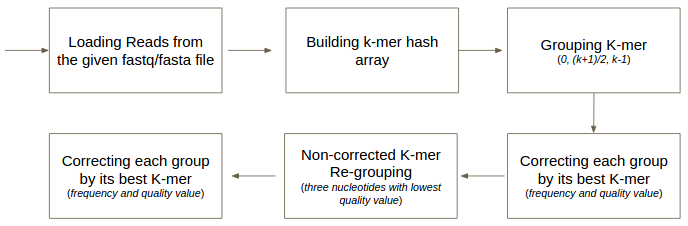
\includegraphics[width=1.6\linewidth]{./figs/First-Proposal-1}
	\caption{\label{fig:fig-First-Proposal-1}KGEC Diagram}
\end{figure}

\begin{figure}
\vspace{0.1cm}
\begin{bordered}
Assume a read represented as: $r=s_1s_2\cdots s_n$
\\
Assume k represents the k-mer length
\\
Set code\_a with 0x00
\\
Set code\_c with 0x01
\\
Set code\_g with 0x02
\\
Set code\_t with 0x03
\\
Set gram as uint64\_t with zero value (represents the k-mer)
\\
Set gram\_reverse as uint64\_t with zero value (represents the reverse of k-mer)
\\
Set mask as uint64\_t with ((uint64\_t) 1 $<<$ (2 * k)) - 1 (used in k-mer masking)
\\
Set pre\_gram as uint64\_t with zero value (used in k-mer hashing check)
\\
Set pre\_mask as uint64\_t with zero value (used in k-mer hashing check)
\\
\\
For every nucleotide $s_i$ in $r$ 
\begin{enumerate}
\addtolength{\itemindent}{1cm} 
\item Check the value of $s_i$: 
\vspace{-2mm}
\begin{enumerate}
\addtolength{\itemindent}{1cm}

	\item if $s_i$ equals `A' or `a'
	
	\noindent\hspace{1cm}then,
	
	\begin{itemize}
    \addtolength{\itemindent}{1cm}
	  \item Reset gram with: gram $<<$ 2 $|$ code\_a
      \item Reset gram\_reverse with: gram\_reverse $>>$ 2 $|$ code\_t $<<$(k - 1)*2
	\end{itemize}
	
	\item if $s_i$ equals `C' or `c'
	
	\noindent\hspace{1cm}then,

	\begin{itemize}
    \addtolength{\itemindent}{1cm}
	  \item Reset gram with: gram $<<$ 2 $|$ code\_c
	  \item Reset gram\_reverse with: gram\_reverse $>>$ 2 $|$ code\_g $<<$(k - 1)*2
	\end{itemize}
	
	\item if $s_i$ equals `G' or `g'
	
	\noindent\hspace{1cm}then,

	\begin{itemize}
    \addtolength{\itemindent}{1cm}	
     	\item Reset gram with: gram $<<$ 2 $|$ code\_g
      	\item Reset gram\_reverse with: gram\_reverse $>>$ 2 $|$ code\_c $<<$(k - 1)*2
	\end{itemize}
	
	\item if $s_i$ equals `T' or `t'
	
	\noindent\hspace{1cm}then,

	\begin{itemize}
    \addtolength{\itemindent}{1cm}
      \item Reset gram with: gram $<<$ 2 $|$ code\_t
	  \item Reset gram\_reverse with: gram\_reverse $>>$ 2 $|$ code\_a $<<$(k - 1)*2
	\end{itemize}

\end{enumerate}

\item Reset gram with: gram \& mask

\item Reset gram\_reverse with: gram\_reverse \& mask;

\item Check if $i >$ k, then, check:
\vspace{-2mm}
\begin{enumerate}
\addtolength{\itemindent}{1cm}
      \item if gram $<$ gram\_reverse \&\& (gram \& pre\_mask) == pre\_gram
      	
      \noindent\hspace{1cm}then, add a k-mer to the hash array at index mapped to gram
	   
	  \item if gram\_reverse $<$ gram \&\& (gram\_reverse \& pre\_mask) == pre\_gram
	  
      \noindent\hspace{1cm}then, add a k-mer to the hash array at index mapped to gram\_reverse
	  
\end{enumerate}            
End For	
\end{enumerate}
\end{bordered}
\caption{\label{fig:fig-KGEC-HASH}KGEC K-mer Hashing Abstraction}
\end{figure}

\begin{figure}
\vspace{0.1cm}
\begin{bordered}
Assume kmer\_hash\_arr is an array that hold the hashing table with size m
\\
Assume k represents the k-mer length
\\
\\
For every k-mer in kmer\_hash\_arr

\noindent\hspace{0.4cm} Check if this k-mer doesn't belong to any k-mer group

\noindent\hspace{0.4cm} then,

\vspace{-3mm}
\begin{enumerate}
\addtolength{\itemindent}{1cm}
	  \item Initialize a new k-mer group

	  \item Add this k-mer to the new k-mer group

      \item Generate all k-mers having typical nucleotides as this k-mer, except,
      
      \noindent\hspace{1cm} for these positions \{0, (k-1)/2, k-1\}, it may have different nucleotide
      
      \item For every generated k-mer
	
		\noindent\hspace{1.4cm} if the hash of this generated k-mer exists in kmer\_hash\_arr 
		
		\noindent\hspace{1.4cm} then, add this generated k-mer to the new k-mer group created above
		
		\noindent\hspace{1.4cm} else, do nothing
		
		\noindent\hspace{1cm} End For
		
\end{enumerate}            
\vspace{-3mm}

End For
\\
\\
For every k-mer group 

\vspace{-3mm}
\begin{enumerate}
\addtolength{\itemindent}{1cm}
  \item Search for the k-mer with the highest frequency 

  \item Check if there are more than one k-mer having the highest frequency

  \noindent\hspace{1cm} then, set corrective\_kmer as the one with the highest frequency and quality

  \noindent\hspace{1cm} else, set corrective\_kmer as the one with the highest frequency

  \item For every k-mer in this k-mer group

  \noindent\hspace{1.4cm}Mark this k-mer's nucleotides at \{0, (k-1)/2, k-1\} to be corrected 
  
  \noindent\hspace{1.4cm}with their corresponding one in the corrective\_kmer
  
  \noindent\hspace{1cm} End For
\end{enumerate}            
\vspace{-3mm}

End For
\\
\\
For every k-mer in kmer\_hash\_arr

\noindent\hspace{0.4cm} Check if this k-mer doesn't belong to any k-mer group

\noindent\hspace{0.4cm} then,

\vspace{-2mm}
\begin{enumerate}
\addtolength{\itemindent}{1cm}
	  \item Set weak\_positions array to hold the position of the three nucleotides with 
	  
	  \noindent\hspace{1cm}the lowest quality
	  
	  \item Initialize a new k-mer group

	  \item Add the weak\_positions element to the new k-mer group

	  \item Add this k-mer to the new k-mer group

      \item Generate all k-mers having typical nucleotides as this k-mer, except,
      
      \noindent\hspace{1cm} for the positions in weak\_positions, it may have different nucleotide
      
      \item For every generated k-mer
	
		\noindent\hspace{1.4cm} if the hash of this generated k-mer existent in kmer\_hash\_arr 
		
		\noindent\hspace{1.4cm} then, add this generated k-mer to the new k-mer group created above
		
		\noindent\hspace{1cm} End For

\end{enumerate}            
\vspace{-3mm}
End For
\\
\\
For every k-mer group 
\vspace{-3mm}
\begin{enumerate}
\addtolength{\itemindent}{1cm}
  \item Search for the k-mer with the highest frequency 

  \item Check if there are more than one k-mer having the highest frequency

  \noindent\hspace{1cm} then, set corrective\_kmer as the one with the highest frequency and quality

  \noindent\hspace{1cm} else, set corrective\_kmer as the one with the highest frequency

  \item For every k-mer in this k-mer group

  \noindent\hspace{1.4cm}Mark this k-mer's nucleotides at the weak\_positions element of this    
  
  \noindent\hspace{1.4cm}k-mer group to be corrected with their corresponding one in the 
  
  \noindent\hspace{1.4cm}corrective\_kmer
  
  \noindent\hspace{1cm} End For
\end{enumerate}            
\vspace{-3mm}
End For		
\end{bordered}
\caption{\label{fig:fig-KGEC-ALG}KGEC Grouping and Correction Decision Pseudo-Code - O(\textit{$4^m$})}
\end{figure}


\chapter{\label{chap:5}H-RACER Algorithm}
This chapter illustrates the working methodology of H-RACER (the second proposed algorithm) in details, where the pseudo code, flowchart and examples are discussed in details. While the evaluation will be discussed in chapter \ref{chap:6}.
\\
\\
The second proposed algorithm (Hybrid RACER or H-RACER) \cite{HRACER} is the newly proposed algorithm that aims to correct all types of errors. H-RACER follows the same algorithm of RACER in detecting errors and deciding their corrections, the newly added part in H-RACER is the detection of the error type in order to apply the correction properly for datasets with varying error types.

\section{Methodology}
As stated before, H-RACER \cite{HRACER} aims to correct all types of errors (substitution, insertion, and deletion). Although RACER is the fastest DNA error correction algorithm existent nowadays with a high accuracy, but it can not correct all types of errors, it can only correct substitutions. So, H-RACER is proposed in order to correct all types of errors. Hence, it follows the same algorithm of RACER in detecting errors and deciding their corrections, and the newly added part is the detection of the error type in order to apply the correction properly for datasets with varying error types.
\\
\\
H-RACER detects the error type for an erroneous nucleotide by studying its correction value (obtained by RACER) against its neighbours, then decides the corrective action (substitute, insert, delete) according to the detected error type.
Once the error detection and correction stages are done, H-RACER starts applying correction using its own methodology which mainly depends on detecting the error type in order to apply the detected correction with the proper action (substitution, insertion or deletion).
\\
\\
H-RACER starts the error type detection by looping on every nucleotide in the whole reads set, to check if this nucleotide is an erroneous one. For every erroneous nucleotide H-RACER checks if this nucleotide is not the last one in the read (so that there is at least one nucleotide following it) where the follower nucleotide is erroneous too. Then H-RACER starts to examine the erroneous and corrective values for both nucleotides (the current and its follower). H-RACER checks if the correction value of the current erroneous nucleotide is equal to the erroneous value of its follower, so it will be concluded that this current erroneous nucleotide is a result of an insertion erroneous action. Hence, H-RACER applies the correction as a deletion action for this current erroneous nucleotide. But, if it is found that the erroneous value of the current nucleotide is equal to the correct value of its erroneous follower, so it will be concluded that this current erroneous nucleotide is a result of a deletion erroneous action. Hence, H-RACER applies the correction as an insertion action at a position directly before the current erroneous nucleotide with the correction value of it (the current erroneous nucleotide). Otherwise, if there is not any alternative equality relation between the erroneous and correction values of the current nucleotide and its erroneous follower (i.e. the correction/erroneous value of the current erroneous nucleotide is not equal to the erroneous/correction value of its follower), then it will be concluded that this current erroneous is a result of a substitution erroneous action. Hence, H-RACER applies the corrective action as a substitution action for the erroneous value of the current nucleotide with its correction value.
\\
\\
On another side, if it is found that the current nucleotide is the last one in the read or its follower nucleotide is not erroneous, then H-RACER will check the position of this nucleotide in the read not to be the first in the read (so that there is at least one nucleotide that precedes it) where the precedent nucleotide is erroneous too. Then H-RACER starts to examine the erroneous and corrective values for both nucleotides (the current and its precedent). H-RACER checks if the correction value of the current erroneous nucleotide is equal to the erroneous value of its precedent, so it will be concluded that this current erroneous nucleotide is a result of an insertion erroneous action. Hence, H-RACER applies the correction as a deletion action for this current erroneous nucleotide. But, if it is found that the erroneous value of the current nucleotide is equal to the correction value of its erroneous precedent, so it will be concluded that this current erroneous nucleotide is a result of a deletion erroneous action. Hence, H-RACER applies the correction as an insertion action at a position directly after the current erroneous nucleotide with the correction value of it (the current erroneous nucleotide). Otherwise, if there is no criss-cross equality relation between the erroneous and correction values of the current nucleotide and its erroneous precedent (i.e. the correction/erroneous value of the current erroneous nucleotide is not equal to the erroneous/correction value of its precedent), then it will be concluded that this current erroneous is a result of a substitution erroneous action. Hence, H-RACER applies the corrective action as a substitution action for the erroneous value of the current nucleotide with its correction value.
\\
\\
Finally, if H-RACER finds that the current nucleotide is either the last or the first in the read, or neither its follower nor precedent nucleotides are erroneous, then it will be concluded that this current erroneous is a result of a substitution erroneous action. Hence, H-RACER applies the corrective action as a substitution action for the erroneous value of the current nucleotide with its correction value.
\\
\\
H-RACER error detection algorithm has a complexity O(\textit{r}), where \textit{r} is the number of reads. For more illustration check the examples shown below in Fig. \ref{fig:fig-HRACER-EX} and Fig. \ref{fig:fig-HRACER-ABS}, also the flow chart shown in Fig. \ref{fig:fig-Second-Proposal-1} is illustrated in Fig. \ref{fig:fig-Second-Proposal-1} in addition to the pseudo-code shown in Fig. \ref{fig:fig-HRACER-PSC}.

\begin{figure}
\vspace{0cm}
\begin{bordered}
\begin{enumerate}
	\item  \textbf{\underline{Inserted Nucleotide - Deletion Correction}}
	\begin{enumerate}
		\item Read Sequence: AC\underline{GT}$\cdots$
		\item Correction: AC\textbf{T}$\cdots$
		\item Tracing: 
		\begin{enumerate}
			\item \underline{G} is an erroneous nucleotide
			\item \underline{G} is followed by an erroneous nucleotide \underline{T}
			\item \underline{G}'s correction value is \textbf{T}
		\end{enumerate}
		\item Conclusion: \underline{G} is an erroneously inserted nucleotide
	\end{enumerate}
	\item  \textbf{\underline{Deleted Nucleotide - Insertion Correction}}
	\begin{enumerate}
		\item Read Sequence: AC\underline{GT}$\cdots$
		\item Correction: AC\textbf{AG}$\cdots$
		\item Tracing: 
		\begin{enumerate}
			\item \underline{G} is an erroneous nucleotide
			\item \underline{G} is followed by an erroneous nucleotide \underline{T}
			\item \underline{G}'s correction value is \textbf{A}
			\item \underline{T}'s correction value is \textbf{G}
		\end{enumerate}
		\item Conclusion: \textbf{A} is an erroneously deleted nucleotide	
	\end{enumerate}
	\item  \textbf{\underline{Substituted Nucleotide - Substitution Correction}}
	\begin{enumerate}
		\item Read Sequence: AC\underline{GT}$\cdots$
		\item Correction: AC\textbf{AC}$\cdots$
		\item Tracing: 
		\begin{enumerate}
			\item {G} is an erroneous nucleotide
			\item \underline{G} is followed by an erroneous nucleotide \underline{T}
			\item \underline{G}'s correction value is \textbf{A}
			\item \underline{T}'s correction value is \textbf{C}
		\end{enumerate}
		\item Conclusion: \textbf{A} is an erroneously substituted nucleotide with \underline{G}
\\
	\end{enumerate}
\end{enumerate}
\footnotesize{Note: The erroneous nucleotides are the underlined ones, while the nucleotides corrections are the ones in bold.}
\end{bordered}
\caption{\label{fig:fig-HRACER-EX}H-RACER Error Type Detection Examples}
\end{figure}

\begin{figure}
\vspace{0.1cm}
\begin{bordered}
Assume a read represented as: $r=s_1s_2\cdots s_n$
\\
if $s_i$ is erroneous
\\
Then,
\begin{enumerate}
	\item if $s_{i+1}$ has error
	Then,
	\begin{enumerate}
		\item Delete $s_{i}$, if the correction of $s_{i}$ equals to $s_{i+1}$
		\item Insert the correction of $s_{i}$ before $s_{i}$, if $s_{i}$ equals to the correction of $s_{i+1}$
		\item Substitute $s_{i}$ with its correction, otherwise 
	\end{enumerate}
	\item if $s_{i-1}$ has error
	Then,
	\begin{enumerate}
		\item Delete $s_{i}$, if the correction of $s_{i}$ equals to $s_{i-1}$
		\item Insert the correction of $s_{i}$ after $s_{i}$, if $s_{i}$ equals to the correction of $s_{i-1}$
		\item Substitute $s_{i}$ with its correction, otherwise 
	\end{enumerate}
\end{enumerate}
\end{bordered}
\caption{\label{fig:fig-HRACER-ABS}H-RACER Error Type Detection Abstraction}
\end{figure}

\begin{figure}
	\centerfloat
	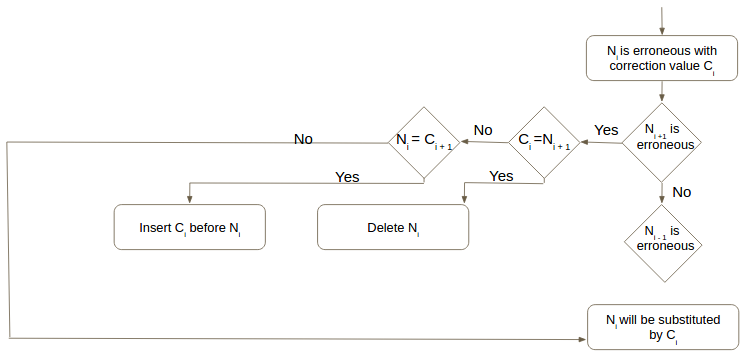
\includegraphics[width=1.3\linewidth]{./figs/Second-Proposal-1}
	\caption{\label{fig:fig-Second-Proposal-1}H-Racer Flow Chart}
\end{figure}


\begin{figure}
\vspace{0.2cm}
\begin{bordered}
\noindent\hspace{3ex}for every \textit{read} in \textit{reads} do

\noindent\hspace{6ex}for every \textit{nuc} in \textit{read} do

\noindent\hspace{9ex}if has\_error(\textit{nuc})

\noindent\hspace{12ex}if not\_last(\textit{nuc}) AND has\_error(next(\textit{nuc}))

\noindent\hspace{15ex}if correction(\textit{nuc}) equals to next(\textit{nuc})

\noindent\hspace{18ex}Delete \textit{nuc} from read

\noindent\hspace{15ex}else if \textit{nuc} equals to correction(next(\textit{nuc}))

\noindent\hspace{18ex}Insert correction(\textit{nuc}) before \textit{nuc} in read

\noindent\hspace{15ex}else 

\noindent\hspace{18ex}substitute \textit{nuc} with correction(\textit{nuc}) in read

\noindent\hspace{15ex}end if

\noindent\hspace{12ex}else if not\_first(\textit{nuc}) AND has\_error(previous(\textit{nuc}))

\noindent\hspace{15ex}if correction(\textit{nuc}) equals to previous(\textit{nuc})

\noindent\hspace{18ex}Delete \textit{nuc} from read

\noindent\hspace{15ex}else if \textit{nuc} equals to correction(previous(\textit{nuc}))

\noindent\hspace{18ex}Insert correction(\textit{nuc}) after \textit{nuc} in read

\noindent\hspace{15ex}else 

\noindent\hspace{18ex}substitute \textit{nuc} with correction(\textit{nuc}) in read

\noindent\hspace{15ex}end if		

\noindent\hspace{12ex}else 

\noindent\hspace{15ex}substitute \textit{nuc} with correction(\textit{nuc}) in read

\noindent\hspace{12ex}end if

\noindent\hspace{9ex}end if

\noindent\hspace{6ex}end for 

\noindent\hspace{3ex}end for 
\end{bordered}
\caption{\label{fig:fig-HRACER-PSC}H-RACER Pseudo-Code - O(\textit{r})}
\end{figure}
\newpage

\chapter{\label{chap:6}Experimental Results}
The evaluation chapter has two main sections. The first section illustrates the characteristics of the used datasets and how far they vary. While in the second section shows a discussion for the results of the comparison tests established between each of the proposed algorithms (KGEC and H-RACER) and the other existent algorithms in details.
\section{\label{sec:eval-data}Datasets and Platform}
The testing of both proposed algorithms was performed on a wide variety of real datasets, shown below in table \ref{tab:eval-data}, with different read length, genome size and coverage. It was preferred to use real datasets and to avoid any simulated ones as they do not offer a good indication of real life performance. 
\\
The testing datasets were selected to have variety in the lengths of the genome and the reads in addition to the number of reads and the reads coverage. ``Lactococcus Lactis" represents the smallest dataset in the running time, as its number of reads multiplied by its reads length shows the smallest number of nucleotides to be processed in comparison with the other datasets.
While ``Treponema Pallidum" represents the dataset with the highest coverage rate (hence the highest ambiguity), as its number of reads multiplied by its reads length divided by the genome length shows the highest value compared to the other datasets.
About ``E.coli 75a", it is a little bit larger dataset with the smallest coverage rate in comparison with other datasets. And finally, ``E.coli 75b" represents the largest dataset in the running time, as its number of reads multiplied by its reads length shows the smallest number of nucleotides to be processed in comparison with the other datasets.
\\
All datasets were brought from the National Center for Biotechnology Information (NCBI).
\\
All algorithms were executed on the same amazon elastic cloud (AWS EC2) instance with 32 vCPU and 244GiB RAM, with Linux (Ubuntu) operating system.

\begin{longtable}{|m{22mm}|m{21mm}|m{23mm}|m{16.5mm}|m{12mm}|m{17mm}|m{16mm}|}
	    \caption{\label{tab:eval-data}Datasets used in evaluation} \\
        \hline
        Name & Accession Number & Genome & Genome Length & Read Length & Number of Reads & Coverage\TBstrut\\ % top and bottom struts
        \hline
        Lactococcus Lactis & SRR088759 & NC\_013656.1 & 2,598,144 & 36 & 4,370,050 & 60.55\TBstrut\\ % top and bottom struts
        \hline
        Treponema Pallidum & SRR361468 & CP002376.1 & 1,139,417 & 35 & 7,133,663 & 219.13\TBstrut\\ % top and bottom struts
        \hline
        E.coli 75a & SRR396536 & NC\_000913.2 & 4,639,675 & 75 & 3,454,048 & 55.83\TBstrut\\ % top and bottom struts
        \hline
        E.coli 75b & SRR396532 & NC\_000913.2 & 4,639,675 & 75 & 4,341,061 & 70.17\TBstrut\\ % top and bottom struts
        \hline
\end{longtable}

\section{Results}
\subsection{\label{subsec:eval1-res}K-mer Grouping Error Correction Algorithm}
The comparisons, shown below in table \ref{tab:eval-0}, were established between K-mer Grouping Error Correction (KGEC) and the algorithms specialized in correcting all types of errors (substitutions, insertions, and deletions). While the obtained measurements were brought via the verification code implemented by RACER \cite{Racer}, that has the advantage of avoiding the interference of mapping or assembling programs. 
\\\\
For Lactococcus Lactis, the data with smallest size, the proposed algorithm shows the best accuracy with a very small difference (0.05\%), but with the worst time with a big difference; 1 hr compared to 15, 5, and 3 mins.
\\
\\
While for Treponema Pallidum, data with larger size, the algorithm has been running for more than 16 hrs compared to 22, 12, and 3 mins; which enforced the interruption of the running without getting the results.
\\
\\
For E.coli 75a and E.coli 75b, the largest dataset, the algorithm has been running for a day (24 hrs) without completion; which enforced the interruption of the running without getting the results.
\\
\\
The defect in time of this algorithm caused from the k-mers grouping steps illustrated above in chapter \ref{chap:4} specifically in section \ref{sec:alg1-meth}, where the algorithm is mainly dependent on the k-mers grouping, and the kmers grouping takes place by generating all of the possible cases of the corrections of every kmer, and here goes the time defect, as the complexity of the k-mers grouping step in exponential of the k-mers count.
\\
\\
The main major step of the proposal implies to its weakness point, which proves that this proposal will not get a better results, and in practice, some trials were done in order to replace the k-mers grouping and consequently the removal of the exponential complexity but it negatively affects the accuracy.

\begin{longtable}{|m{33mm}|m{20mm}|m{20mm}|m{20mm}|m{20mm}|}
	    \caption{\label{tab:eval-0}KGEC - Evaluation comparison table for Lactococcus Lactis}\\
        \hline
           & Coral & Pollux & HSHSREC & H-RACER\cellcolor{DarkGray} \TBstrut\\ % top and bottom struts
        \hline
           Accuracy & 91.45\% & 94.15\% & 95.34\% & 95.39\%\cellcolor{LightGray} \TBstrut\\ % top and bottom struts
        \hline
           Time in Minutes& 5 & 3 & 15 & 61\cellcolor{LightGray} \TBstrut\\ % top and bottom struts
        \hline
\end{longtable}


\subsection{\label{subsec:eval2-res}H-RACER Algorithm}
The comparisons, shown below in tables \ref{tab:eval-1}, \ref{tab:eval-2}, \ref{tab:eval-3}, and \ref{tab:eval-4}, were established between H-RACER and the algorithms specialized in correcting all types of errors (substitutions, insertions, and deletions). While the obtained measurements were brought via the verification code implemented by RACER \cite{Racer}, that has the advantage of avoiding the interference of mapping or assembling programs. 
\\\\
As shown below in the comparisons tables, H-RACER has the best results in accuracy and time. Actually, H-RACER aims to increase the genome reads accuracy, consequently, it aims to eliminate the errors existing in the genome reads. So, H-RACER avoided introducing errors to the reads by lowering the false positive rate and consequently increasing the specificity rate (as illustrated before by equation \ref{eq:specificity}). On the other side, the false negative rate was negatively affected and the sensitivity rate was decreased as well. But, this approach did not negatively affect the accuracy, on contradictory, it resulted in getting the best accuracy.
\\
In other words, the high accuracy of H-RACER mainly resulted from both, the remarkable lowering of false positive rate and the high raising of true negative rate (where the false positive rate is inversely proportional with the true negative one). On the other side, both, the true positive and false negative rates were negatively affected. Hence, H-RACER does not have neither the highest true positive nor the lowest false positive rates. And this is what H-RACER follows in RACER's footsteps, where it is preferred to lower the algorithm sensitivity represented in raising the false negative rate and lowering the true positive rate rather than raising the false positive rate and lowering the true negative rate. And this makes sense, as enhancing the reads overall accuracy is the main vital target. So, corrective algorithms should not introduce errors (represented in false positive rate), but it should target a higher gain to get higher accuracy, and so does RACER followed by H-RACER.
\\\\
The comparisons with the other algorithms, shown below in tables \ref{tab:eval-1}, \ref{tab:eval-2}, \ref{tab:eval-3}, and \ref{tab:eval-4}, prove that although the other algorithms have higher sensitivity than H-RACER, but all of them do not explicitly beat H-RACER accuracy, except for \enquote{Treponema Pallidum}, where HSHREC beats H-RACER's accuracy by 0.07\% and this is due to the high coverage rate of \enquote{Treponema Pallidum} that will be explained below.  
\\\\
For the short genome \enquote{Lactococcus Lactis}, illustrated in table \ref{tab:eval-1}, H-RACER shows the best results in specificity, gain, accuracy and time compared to CORAL, Pollux and HSHREC, although the sensitivity of H-RACER is not the best. But H-RACER gains the highest accuracy by lowering the false positive rate (as explained above).
\\\\ 
For \enquote{Treponema Pallidum}, the short genome with a very high coverage (the average number of reads representing a given nucleotide in the reconstructed sequence) as illustrated in tables \ref{tab:eval-data} and \ref{tab:eval-2}, H-RACER shows a lowering in the true positive rate with a raising in the false negative one rather than the expected rates. This is due to the very high coverage of \enquote{Treponema Pallidum} that increases the ambiguity for H-RACER in detecting the proper correction for some nucleotides, leading to a lowering in the true positive rate and consequently in the accuracy. But, by comparing such an accuracy with others, as illustrated in table \ref{tab:eval-2}, it is obvious that H-RACER shows the best results in specificity, gain, accuracy and time compared to CORAL and Pollux. While HSHREC is the only algorithm that beats H-RACER's gain and accuracy (for \enquote{Treponema Pallidum} only) with a very little difference rates (0.29\% and 0.07\% respectively). But, H-RACER accomplished such a correction in the best time compared to all others including HSHREC's (with a very remarkable ratio) and the best specificity as well.
\\\\
For long genomes \enquote{E.coli 75a} and \enquote{E.coli 75b}, illustrated in tables \ref{tab:eval-3} and \ref{tab:eval-4}, H-RACER obviously shows the best results in accuracy with a very perfect time, while CORAL and Pollux show lower accuracy with too much longer time, but HSHREC's running throws exception for such genomes, as SHREC (and consequently HSHREC) requires a very large space \cite{Racer}, \cite{HShrec}, so it is unable to run successfully for the larger genomes on the specified machine.
\\\\ 
Finally, the remarkable great difference in time between H-RACER and the rest of the algorithms is due to the bitwise orientation in implementation (inherited from RACER), and also H-RACER keeps RACER's complexity, consequently, H-RACER gains the advantage of having the best time. 

\begin{longtable}{|m{33mm}|m{20mm}|m{20mm}|m{20mm}|m{20mm}|}
	    \caption{\label{tab:eval-1}H-RACER - Evaluation comparison table for Lactococcus Lactis}\\
        \hline
           & Coral & Pollux & HSHSREC & H-RACER\cellcolor{DarkGray} \TBstrut\\ % top and bottom struts
        \hline
           True Positive & 15,396,336 &  25,325,532 & 25,537,644 & 21,237,660\cellcolor{LightGray} \TBstrut\\ % top and bottom struts
        \hline
           False Positive & 2,039,148 &  7,720,920 & 6,053,580 & 19,656\cellcolor{LightGray} \TBstrut\\ % top and bottom struts
        \hline
           False Negative & 11,413,764 & 1,484,568 & 1,272,456 & 5,572,440\cellcolor{LightGray} \TBstrut\\ % top and bottom struts
        \hline
           True Negative & 128,472,552 & 122,790,780 & 124,458,120 & 130,492,044\cellcolor{LightGray} \TBstrut\\ % top and bottom struts
        \hline
           Sensitivity & 57.43\% & 94.46\% & 95.25\% & 79.22\%\cellcolor{LightGray} \TBstrut\\ % top and bottom struts
        \hline
           Specificity & 98.44\% & 94.08\% & 95.36\% & 99.98\%\cellcolor{LightGray} \TBstrut\\ % top and bottom struts
        \hline
           Gain & 49.82\% & 65.66\% & 72.67\% & 79.14\%\cellcolor{LightGray} \TBstrut\\ % top and bottom struts
        \hline
           Accuracy & 91.45\% & 94.15\% & 95.34\% & 96.45\%\cellcolor{LightGray} \TBstrut\\ % top and bottom struts
        \hline
           Time in Minutes& 5 & 3 & 15 & 1\cellcolor{LightGray} \TBstrut\\ % top and bottom struts
        \hline
\end{longtable}
\newpage
\begin{longtable}{|m{33mm}|m{20mm}|m{20mm}|m{20mm}|m{20mm}|}
	    \caption{\label{tab:eval-2}H-RACER - Evaluation comparison table for Treponema Pallidum}\\
        \hline
           & Coral & Pollux & HSHSREC & H-RACER\cellcolor{DarkGray} \TBstrut\\ % top and bottom struts
        \hline
           True Positive & 25,553,185 & 63,845,425 & 64,381,905 & 56,277,270\cellcolor{LightGray} \TBstrut\\ % top and bottom struts
        \hline
           False Positive & 3,462,165 & 8,832,320 & 8,133,895 & 223,405\cellcolor{LightGray} \TBstrut\\ % top and bottom struts
        \hline
           False Negative & 41,547,065 & 3,254,825 & 2,718,345 & 10,822,980\cellcolor{LightGray} \TBstrut\\ % top and bottom struts
        \hline
           True Negative & 179,115,790 & 173,745,635 & 174,444,060 & 182,354,550\cellcolor{LightGray} \TBstrut\\ % top and bottom struts
        \hline
           Sensitivity & 38.08\% & 95.15\% & 95.95\% & 83.87\%\cellcolor{LightGray} \TBstrut\\ % top and bottom struts
        \hline
           Specificity & 98.10\% &  95.16\% & 95.55\% & 99.88\%\cellcolor{LightGray} \TBstrut\\ % top and bottom struts
        \hline
           Gain & 32.92\% & 81.99\% & 83.83\% & 83.54\%\cellcolor{LightGray} \TBstrut\\ % top and bottom struts
        \hline
           Accuracy & 81.97\% & 95.16\% & 95.65\% & 95.58\%\cellcolor{LightGray} \TBstrut\\ % top and bottom struts
        \hline
           Time in Minutes& 12 & 3 & 22 & 2\cellcolor{LightGray} \TBstrut\\ % top and bottom struts
        \hline
\end{longtable}
\newpage
\begin{longtable}{|m{33mm}|m{20mm}|m{20mm}|m{20mm}|m{20mm}|}
	    \caption{\label{tab:eval-3}H-RACER - Evaluation comparison table for E.coli 75a}\\
        \hline
           & Coral & Pollux & HSHSREC & H-RACER\cellcolor{DarkGray} \TBstrut\\ % top and bottom struts
        \hline
           True Positive & 26,434,125 & 79,984,425 & N/A & 76,325,475\cellcolor{LightGray} \TBstrut\\ % top and bottom struts
        \hline
           False Positive & 5,549,925 & 31,675,650 & N/A & 33,000\cellcolor{LightGray} \TBstrut\\ % top and bottom struts
        \hline
           False Negative & 73,707,075 & 20,164,125 & N/A & 23,823,075\cellcolor{LightGray} \TBstrut\\ % top and bottom struts
        \hline
           True Negative & 153,362,475 & 127,229,400 & N/A & 158,872,050\cellcolor{LightGray} \TBstrut\\ % top and bottom struts
        \hline
           Sensitivity & 26.40\% & 79.87\% & N/A & 76.21\%\cellcolor{LightGray} \TBstrut\\ % top and bottom struts
        \hline
           Specificity & 96.51\% & 80.07\% & N/A & 99.98\%\cellcolor{LightGray} \TBstrut\\ % top and bottom struts
        \hline
           Gain & 20.85\% & 48.24\% & N/A & 76.18\%\cellcolor{LightGray} \TBstrut\\ % top and bottom struts
        \hline
           Accuracy & 69.40\% & 79.99\% & N/A & 90.79\%\cellcolor{LightGray} \TBstrut\\ % top and bottom struts
        \hline
           Time in Minutes& 9 & 16 & N/A & 1\cellcolor{LightGray} \TBstrut\\ % top and bottom struts
        \hline
\end{longtable}
\newpage
\begin{longtable}{|m{33mm}|m{20mm}|m{20mm}|m{20mm}|m{20mm}|}
        \caption{\label{tab:eval-4}H-RACER - Evaluation comparison table for E.coli 75b}\\
        \hline
           & Coral & Pollux & HSHSREC & H-RACER\cellcolor{DarkGray} \TBstrut\\ % top and bottom struts
        \hline
           True Positive & 13,312,725 & 99,375,600 & N/A & 81,059,700\cellcolor{LightGray} \TBstrut\\ % top and bottom struts
        \hline
           False Positive & 3,681,450 & 37,779,750 & N/A & 35,925\cellcolor{LightGray} \TBstrut\\ % top and bottom struts
        \hline
           False Negative & 108,494,025 & 22,439,925 & N/A & 40,755,825\cellcolor{LightGray} \TBstrut\\ % top and bottom struts
        \hline
           True Negative & 200,091,375 & 165,984,300 & N/A & 203,728,125\cellcolor{LightGray} \TBstrut\\ % top and bottom struts
        \hline
           Sensitivity & 10.93\% & 81.58\% & N/A & 66.54\%\cellcolor{LightGray} \TBstrut\\ % top and bottom struts
        \hline
           Specificity & 98.19\% & 81.46\% & N/A & 99.98\%\cellcolor{LightGray} \TBstrut\\ % top and bottom struts
        \hline
           Gain & 7.91\% & 50.56\% & N/A & 66.51\%\cellcolor{LightGray} \TBstrut\\ % top and bottom struts
        \hline
           Accuracy & 65.55\% & 81.50\% & N/A & 87.47\%\cellcolor{LightGray} \TBstrut\\ % top and bottom struts
        \hline
           Time in Minutes& 13 & 21 & N/A & 2\cellcolor{LightGray} \TBstrut\\ % top and bottom struts
        \hline
\end{longtable}

\newpage
\chapter{\label{chap:7}Conclusion and Future Work}
This chapter has two main sections, the conclusion and the future work. The conclusion section shows a very short briefed discussion about the proposed algorithms. While the future work section shows the major researchable points that can be investigated in the future.
\section{Conclusion}
The next-generation sequencing generated too many short reads in a reasonable time, but unfortunately it introduced too many errors with different type (substitution, insertion and deletion), and the accuracy of the reads decreased. But, accuracy of the output reads is a vital and a necessary factor, where the reads processes, applications and projects depends on it and  it is greatly affected by it. Consequently, fixing the errors and raising reads accuracy is an interesting field with many challenges.
\\
\\
The two proposed algorithms aim to fix all types of nucleotide errors (substitutions, insertions, and deletions) in a mixed set of reads, in order to raise the accuracy of the DNA sequencing output within the shortest time compared to the existent algorithms. 
\\
\\
K-mer Grouping Error Correction (KGEC - the first proposed algorithm) is mainly invented based on k-mers grouping and nucleotide frequencies and quality values. It accomplishes the correction mission properly with a high accuracy for the small dataset, but unfortunately it takes too much long time. Consequently, it is not able to compete for the larger dataset as it needs a very long time, which cannot be enhanced as this negatively effects the accuracy.
\\
\\
H-RACER (the second proposed algorithm) overcomes the time issue of the first algorithm and also it accomplishes the mission successfully, it is able to raise the next-generation sequencing output accuracy. 
\\
\\
H-RACER (the second proposed algorithm) comes up with the advantage of correcting different error types which were missed in RACER. H-RACER followed in the footsteps of RACER's implementation in order to acquire the major advantages of RACER in both aspects performance and time, then added its elegant algorithm in detecting the errors types and properly applying their corrections. Consequently, H-RACER shows great results in both performance and time compared to existent algorithms specialized in correcting all types of errors for large and small genome lengths. And by comparing H-RACER with existent algorithms specialized in correcting all types of errors, it is proved that H-RACER is the fastest with the highest accuracy algorithm.
\\
\\
Finally, both algorithms have been implemented in C/C++ as an open source program.
\\
\\
K-mer Grouping Error Correction (KGEC - the first algorithm) available at: 
\\
- github.com/salmagomaa/DNA-EC/tree/master/4-Best-49g-with-61(Best)
\\
\\
H-RACER (the second algorithm) available at: 
\\
- github.com/salmagomaa/H-RACER
\\
- drive.google.com/open?id=0B7Otgzz7lZlldkE2ZFVwcU5qN1U


\section{Future Work}
As a future work, the main target will be the memory usage enhancement for H-RACER specifically in long genomes, so as to be able to run long genomes within 244GiB RAM.
\\
\\
Also, one of the most interesting point to be added into consideration for the future work is implementing H-RACER with parallel threads, where both time and memory will be enhanced, especially for long genomes.
\\
\\
And finally, K-mer Grouping Error Correction (KGEC - the first proposed algorithm) can get another chance by inventing a new algorithm to group the k-mers in with a reasonable complexity instead of the exponential one.

\newpage

\clearpage\thispagestyle{empty}
% This is LLNCS.DOC the documentation file of
% the LaTeX2e class from Springer-Verlag
% for Lecture Notes in Computer Science, version 2.4
\documentclass[12pt,openany]{llncs}
\usepackage{llncsdoc}
\bibliographystyle{splncs}
%
% PACKAGES	
\usepackage[table]{xcolor}
\usepackage{csquotes}
\usepackage{mdframed}
\usepackage{float}
\usepackage{longtable}
\usepackage{graphicx}
\graphicspath{ {figures/} }
\usepackage{caption}
\usepackage{subcaption}
\usepackage[utf8]{inputenc}
\usepackage[LFE,LAE]{fontenc} 
\usepackage[arabic,english]{babel}
\usepackage{sectsty}

\allsectionsfont{\raggedright}

\captionsetup{compatibility=false}

%Cover page
\newcommand{\HRule}{\rule{\linewidth}{0.5mm}} % Defines a new command for the horizontal lines

\newmdenv[leftline=false,rightline=false,topline=false,bottomline=false,innertopmargin=2pt,innerbottommargin=2pt]{bordered}

% TABLE
\newcommand{\TBstrut}{{\rule{0pt}{7ex}}{\rule[2ex]{0pt}{0pt}}} % top&bottom struts
\definecolor{DarkGray}{gray}{0.6}
\definecolor{LightGray}{gray}{0.9}

\usepackage{tocloft}% http://ctan.org/pkg/tocloft
\setlength{\cftsubsecnumwidth}{4em}% Set length of number width in ToC for \subsection

\usepackage{titlesec}

\titleformat{\chapter}[display]
    {\normalfont\huge\bfseries}{\chaptertitlename\ \thechapter}{2pt}{\Huge}
\titlespacing*{\chapter}{0pt}{0pt}{4pt}

\makeatletter
\newcommand*{\centerfloat}{%
  \parindent \z@
  \leftskip \z@ \@plus 1fil \@minus \textwidth
  \rightskip\leftskip
  \parfillskip \z@skip}
\makeatother
%ABBREVIATIONS
\newcommand{\abbrlabel}[1]{\makebox[4cm][l]{\textbf{#1}\ \dotfill}}
\newenvironment{abbreviations}{\begin{list}{}{\renewcommand{\makelabel}{\abbrlabel}}}{\end{list}}

\begin{document}


\begin{titlepage}
{\small
\center % Center everything on the page

\includegraphics[scale=0.2]{./figs/aast}\\[0.7cm]
\selectlanguage{arabic}
{\large \bfseries 
الاكاديمية العربية للعلوم والتكنولوجيا والنقل البحرى
}\\[0.7cm]
{\large \bfseries 
كلية الحاسبات و تكنولوجيا المعلومات
}\\[1.3cm]
{\LARGE \bfseries 
خوارزميات لتصحيح الأخطاء الناتجة عن عملية تسلسل الحمض النووي
}\\[0.5cm]
{\large \bfseries 
إعداد
}\\[0.3cm]
{\large \bfseries
سلمى محمود محمد جمعة
}\\[0.3cm]
{\bfseries 
رسالة مقدمة للاكاديمية العربية للعلوم والتكنولوجيا والنقل البحرى
}\\[0.2cm]
{\bfseries
لاستكمال متطلبات درجة الماجستير
}\\[0.2cm]
{\bfseries
في
}\\[0.2cm]
{\large \bfseries
علوم الحاسب 
}\\[0.3cm]
{\large \bfseries 
إشراف
}\\[0.3cm]
\begin{minipage}{0.55\textwidth}
{\large \bfseries 
أ. د. ياسر علاء الدين السنباطى
}
\end{minipage}
~
\begin{minipage}{0.40\textwidth}
{\large \bfseries 
د. نهلة أحمد بلال
}
\end{minipage}
\\[0.1cm] 
\begin{minipage}{0.48\textwidth}
\begin{flushleft}
\center
{
أستاذ بكلية الحاسبات وتكنولوجيا المعلومات
}\\
{
الاكاديمية العربية للعلوم والتكنولوجيا والنقل البحرى
}
\end{flushleft}
\end{minipage}
~
\begin{minipage}{0.48\textwidth}
\begin{flushright}
\center
{
مدرس بكلية الحاسبات وتكنولوجيا المعلومات
}\\
{
الاكاديمية العربية للعلوم والتكنولوجيا والنقل البحرى
}
\end{flushright}
\end{minipage}\\[0.5cm]
{
 الاكاديمية العربية للعلوم والتكنولوجيا والنقل البحرى
}\\[0.1cm] 
{\bfseries
 7102
}\\[0cm]


\vfill % Fill the rest of the page with whitespace
}

\clearpage\thispagestyle{empty}

\selectlanguage{arabic}
\section*{ملخص}
إن عملية تسلسل الحمض النووي تعد من أكثر المجالات حيوية في علم الأحياء الحاسوبي. فإن معظم العمليات المرتبطة بالحمض النووي تعتمد في الأساس على عملية تسلسله؛ و من ثم أصبحت كلاً من تكلفة عملية التسلسل, و دقتها، و الوقت المستغرق فيها من العوامل الأساسية الهامة التي يقام عليها العديد من الأبحاث لتحسينها.
\\
\\
إن الهدف الأساسي للجيل الجديد من آليات تسلسل الحمض النووي هو تخفيض تكلفة عملية تحليل المحتوى الوراثي (الجينوم) الضخمة، و الإكثار من إنتشارها أيضاً؛ حيث إن تلك الآليات لديها القدرة على إنتاج العديد من القراءات القصيرة في وقت وجيز؛ و لكن من أهم الآثار الجانبية لتلك السرعة هي قصر طول القراءات مما أدى إلى وجود العديد من الأخطاء على مستوى النواة بأشكال مختلفة؛ مثل خطأ الناتج عن إبدال النواة، و الخطأ الناتج عن إدخال نواة جديدة، و أخيرا الخطأ الناتج عن حذف النواة. و تمثل كل هذه الأخطاء عقبة كبيرة تعوق إستخدام القراءات في المشاريع القائمة على التسلسل (مثل:  عملية تجميع القراءات، و عملية محاذاة المحتوى الوراثي (الجينوم)، إلخ)؛ لذلك أصبحت عملية تصحيح الأخطاء مهمة للغاية حيث إنها تعمل على تخفيض معدل الأخطاء على مستوى القراءات جميعاً؛ و من ثم أصبحت عملية تصحيح جميع أنواع الأخطاء أكثر تحدياً.
\\
\\ 
 تعد الخوارزميات المقدمة في تلك الرسالة من الآليات الجديدة التى تعمل على تصحيح جميع أنواع أخطاء التي تتعرض لها النواة (الإبدال، و الإدخال، و الحذف)؛ فكلتا الآليتين تعمل على زيادة الدقة الخاصة بناتج عملية تسلسل الحمض النووي في أقصر وقت ممكن مقارنة بالخوارزميات المجودة حالياً.
\\
\\
الخوارزم الأول يعتمد على إقامة مجموعات من نتاج تجزئة القراءات حيث يعتمد قرار التصحيح على تكرارات النوى. تلك الآلية قدمت دقة عالية لمجموعة البيانات الصغيرة؛ و لكنها عجزت عن إكمال مهمتها لتلك المجموعات الكبيرة؛ حيث إنها تحتاج لوقت طويل جداً ، بالإضافة إلى أن محاولة تحسين الوقت أثرت سلبياً على عامل الدقة.
\\
\\
 بينما تغلب الخوارزم الثاني على مشكلة الوقت التي أعاقت الخوارزم الأول بالإضافة أنه حقق الهدف الأساسي ألا و هو زيادة الدقة لناتج عملية تسلسل الحمض النووي. تلك الآلية تعتمد في إكتشاف الأخطاء و تقرير قيمة تصحيحه على الخوازم المسمى 
 \selectlanguage{english}RECAR 
 \selectlanguage{arabic}؛ حيث أن الميزة الرئيسية في تلك الآلية هي قدرتها على إكتشاف نوع الخطأ و من ثم تطبيق الإجراء التصحيحي المناسب. لذلك تلك الآلية لديها القدرة على تصحيح جميع أنواع الأخطاء بدقة عالية في أقصر وقت ممكن مقارنةً بالخوارزميات الموجودة حالياً المختصة بتصحيح جميع أنواع الأخطاء.

%%%%%END ABSTRACT

\clearpage\thispagestyle{empty}

\selectlanguage{english}
{
\center % Center everything on the page

\includegraphics[scale=0.2]{./figs/aast}\\[0.7cm]
{\Large \bfseries Arab Academy for Science, Technology and Maritime Transport \\[0.2cm](AAST)}\\[0.2cm]
{\large \bfseries College of Computing and Information Technology}\\[0.3cm]
{\large \bfseries Computer Science Department}\\[0.3cm] 
\HRule \\[0.2cm]
{\LARGE \bfseries DNA Sequencing Error Correction Algorithms}\\[0.1cm]
\HRule \\[0.2cm]
{\large \bfseries A Thesis}\\[0.2cm]
{\large \bfseries Submitted in Partial Fulfillment to the Requirements for the}\\[0.2cm]
{\Large \bfseries Master of Computer Science}\\[0.5cm]
{\large \bfseries Submitted by:}\\[0.2cm]
{\Large \bfseries Salma Mahmoud Mohamed Gomaa}\\[0.5cm]
{\large \bfseries Under Supervision of}\\[0.2cm]

\begin{minipage}{0.55\textwidth}
{\large \bfseries Prof.Dr.Yasser El-Sonbaty}
\end{minipage}
~
\begin{minipage}{0.40\textwidth}
{\large \bfseries Dr.Nahla A. Belal}
\end{minipage}\\[0.2cm]

\begin{minipage}{0.47\textwidth}
\begin{flushleft}
\center
{\small Professor of Computer Science}\\
{\small Arab Academy for Science, Technology, and Maritime Transport}
\end{flushleft}
\end{minipage}
~
\begin{minipage}{0.47\textwidth}
\begin{flushright}
\center
{\small Assistant Professor of Computer Science}\\
{\small Arab Academy for Science, Technology, and Maritime Transport}
\end{flushright}
\end{minipage}\\[0.2cm]
{\small June - 2017}\\[0cm] 
\vfill % Fill the rest of the page with whitespace
}
\clearpage\thispagestyle{empty}

\selectlanguage{english}
\section*{Abstract}
DNA sequencing is one of the very pivotal research fields in bioinformatics. Most of the processes that are related to the DNA genomes mainly depend on the DNA sequencing, and consequently the cost, the accuracy and the time of the DNA sequencing methodologies became very urgent and vital factors, that many researches are being done to enhance these critical factors.
\\
\\
The main targets of the next-generation sequencing technologies are: making the vast analysis of genomes less expensive and more spread, hence, they are able to produce large sets of short reads within a very efficient time. But, as a side effect of this fastness, the produced short reads are subject to be infected by different types of errors on the nucleotide level; such as nucleotide erroneous substitution, nucleotide erroneous insertion and nucleotide erroneous deletion. Since, these errors represent a great obstacle to utilize the reads in sequencing projects (such as: reads assemblers, genome aligners, etc.), the error correction process becomes a vital and essential action that aims to reduce the error rate over the whole reads set. So, the correction of all types of the nucleotides errors becomes very challenging.
\\
\\ 
The proposed algorithms are new error correcting tools that fix all types of nucleotide errors (substitutions, insertions, and deletions) in a mixed set of reads, where both of them aim to raise the accuracy of the DNA sequencing output, trying to accomplish the correction within a suitable time compared to the existent algorithms. 
\\
\\
K-mer Grouping Error Correction (KGEC - the first proposed algorithm) is mainly invented based on k-mers grouping and nucleotide frequencies. It shows a high accuracy for the small dataset but unfortunately it cannot compete for the larger dataset as it needs a very long time, which cannot be enhanced as this negatively effects the accuracy.
\\
\\
H-RACER (the second proposed algorithm) overcomes the time issue of the first algorithm using a large memory space and also it accomplishes the main target which is raising the sequencing output accuracy. It mainly depends on RACER algorithm in detecting the erroneous nucleotide and deciding its corrective value. While the major advantage presented by H-RACER is the detection of the nucleotide corrective action and applying it. So, H-RACER is able to correct the nucleotides substitutions errors as well as their insertions and deletions errors with the highest accuracy and the least time compared to other existent algorithms that specialize in correcting these types of nucleotides errors.

%%%%%END ABSTRACT
\end{titlepage}

\clearpage\thispagestyle{empty}
\section*{Acknowledgement}

I would like to seize this opportunity to express my sincere gratitude for the
unconditional and unlimited help and support that I have received from my supervisors Prof.
Dr. Yasser El-sonbaty and Dr. Nahla Belal. Their continuous guidance and tutoring were
critical for the successful completion of this thesis. Great part of the success of this research stems from the open access to the academy various facilities. 
\\
\\
All Gratitude is first due to ALLAH. Then, I'm deeply grateful for my father, my mother, my husband and my sisters for their enormous support in all aspects. Their continuous encouragement and motivation were the key for overcoming the obstacles encountered during the course of this research. I will be grateful forever for your love.
\\
\\
You all make the journey worthwhile .... Thank you all
\\
\\
\begin{flushright}
Salma Mahmoud Mohamed Gomaa\\
Computer Science, AASTMT,\\
June - 2017
\end{flushright}

\clearpage\thispagestyle{empty}
\section*{Published Work}
\noindent\hspace{0.6cm}The work in this thesis is published in one paper as follow:
\\
\\
Gomaa, S., Belal, N.A. and El-Sonbaty, Y.: H-RACER: Hybrid RACER to Correct Substitution, Insertion, and Deletion Errors. In International Conference on Bioinformatics and Biomedical Engineering (pp. 62-73). Springer, Cham (2017).

\newpage
\tableofcontents
\newpage
\listoffigures
\newpage
\listoftables
\newpage

{\Huge\bfseries List of Abbreviations}
\\
\begin{abbreviations}
\item[AWS EC2] Amazon Elastic Cloud
\item[Coral] Correction with Alignments
\item[CUDA] Compute Unified Device Architecture
\item[DNA] Deoxyribonucleic Acid
\item[EC] Error Corrector
\item[FN] False Negative
\item[FP] False Positive
\item[HiTEC] High Throughput Error Correction
\item[HSHREC] Hybrid Short Read Error Correction
\item[H-RACER] Hybrid RACER
\item[KGEC] K-mer Grouping Error Correction
\item[MSA] Multiple Sequence Alignments
\item[NGS] Next-generation Sequencing
\item[Pollux] Platform Independent Error Correction of 

\noindent\hspace{3.6cm}Single and Mixed Genomes
\item[Quake] Quality-aware Detection and Correction of 

\noindent\hspace{3.6cm}Sequencing Errors
\item[RACER] Rapid and Accurate Correction of Errors in 

\noindent\hspace{3.6cm}Reads
\item[Reptile] Representative Tiling for Short Read Error

\noindent\hspace{3.6cm}Correction
\item[TN] True Negative
\item[TP] True Positive
\end{abbreviations}

\chapter{\label{chap:1} Introduction}
This chapter gives a brief introduction to the thesis. It has three major sections, where it illustrates the problem statement, the thesis objective, and the thesis structure.
\\
\\
In bioinformatics, the DNA sequencing is one of the very pivotal research fields. Many researches has been done in order to enhance the DNA sequencing methodologies, as most of the processes that are related to the DNA genomes mainly depend on the DNA sequencing. So the cost, the accuracy and the time of the DNA sequencing methodologies became very urgent and vital factors, where the target of the researches is to enhance these critical factors.
\section{Problem Statement}
The next-generation sequencing (NGS) high-throughput technologies \cite{NGS} were originally proposed to make the vast analysis of genomes less expensive and more spread. So, their main target is the generation of too many reads in an efficient time. But unfortunately, this leads to negatively affecting the read length and the accuracy, where the read length becomes much shorter than the conventional sequencing, and the accuracy of the generated reads is decreased. 
\\
\\
In the generated reads, each erroneous nucleotide can be introduced to the read sequence via one of the three erroneous actions; which are substitution, insertion and deletion. 
The substitution erroneous action takes place when the nucleotide is substituted or replaced with another erroneous nucleotide. While the insertion erroneous action is the insertion or injection of a newly erroneous nucleotide into the read sequence. Finally, the deletion erroneous action results from the deletion or removal of a proper nucleotide from the read sequence.
\\
\\
The reads accuracy is a very vital factor, since, all of the processes, applications and projects that can be applied on the reads are affected by their accuracy. As an example, the assembly of next-generation sequencing (NGS) reads can not be accomplished successfully until the reads errors are corrected or eliminated. So detecting and correcting (or eliminating) the reads errors is an essential step that should precede the assembly process. 
\\
\\
In most of the error correction methodologies, the erroneous nucleotide detection and its correction value decision mainly depends on the nucleotide frequency with its quality value\cite{ErrCorr}. While, the error correction methodology itself can be accomplished either by a standalone solution or implicitly within the assembly mechanism. 

\section{Objective}
The newly proposed error correction methodologies aim to correct all types of errors (substitutions erroneous action, insertions erroneous action, and deletions erroneous action) in order to enhance the reads accuracy within a suitable time.
\\
Hence, the main objectives can be listed as:
\begin{itemize}
	\item Raising the DNA reads accuracy

	\item Correcting all of the different types of errors

	\item Accomplishing the correction process within the shortest time
\end{itemize}
The first algorithm has the ability to enhance the accuracy, but unfortunately it takes too much time to accomplish his mission. The analysis of the results and time of this proposal will be illustrated later in the following chapters. 
\\
While the second algorithm builds its correction decisions based on RACER \cite{Racer} (an already existent algorithm that handles substitution errors only and will be discussed in details later) with some tuning to handle the insertions and deletions errors. This algorithm has the ability to enhance both the accuracy and the time, as it shows almost the highest accuracy with the shortest time for different datasets in comparison with the existent algorithms specialized in correcting substitution, insertion and deletion errors.

\section{Thesis Structure}
This thesis documentation is organized as follows; illustrating some basics about deoxyribonucleic acid (DNA), deoxyribonucleic acid (DNA) sequencing, next-generation sequencing (NGS), and next-generation sequencing (NGS) errors correction in chapter \ref{chap:2}, while the  existing methodologies for error correction are demonstrated in chapter \ref{chap:3}, then the methodology of K-mer Grouping Error Correction (KGEC - the first proposed algorithm) is demonstrated in chapter \ref{chap:4}, while the methodology of H-RACER (the second proposed algorithm) is demonstrated in chapter \ref{chap:5}. In chapter \ref{chap:6}, the evaluation of both algorithms (K-mer Grouping Error Correction and H-RACER) are illustrated, where the comparisons set using experimental data. The conclusion and future work are shown in chapter \ref{chap:7}.
%

\newpage
\chapter{\label{chap:2}Background}
This chapter has five major sections, where it illustrates some basic information about deoxyribonucleic acid (DNA), DNA sequencing, next-generation sequencing (NGS) and NGS errors correction, in addition it shows the definition of the main concepts and terms used in NGS errors correction field.
\section{Deoxyribonucleic Acid}
Deoxyribonucleic Acid,or DNA  (Fig. \ref{fig:fig-DNA-1}), is the hereditary material in humans and almost all other organisms. Nearly every cell in an organism’s body has the same DNA. Most DNA is located in the cell nucleus (where it is called nuclear DNA) \cite{DNA1,DNA2}.
The information in DNA is stored as a code made up of four chemical bases: adenine (A), guanine (G), cytosine (C), and thymine (T). Human DNA consists of about 3 billion bases \cite{DNA4}, and more than 99 percent of those bases are the same in all people. The order, or sequence, of these bases determines the information available for building and maintaining an organism, similar to the way in which letters of the alphabet appear in a certain order to form words and sentences.
DNA bases pair up with each other, A with T and C with G, to form units called base pairs. Each base is also attached to a sugar molecule and a phosphate molecule. Together, a base, sugar, and phosphate are called a nucleotide. Nucleotides are arranged in two long strands that form a spiral called a double helix. The structure of the double helix is somewhat like a ladder, with the base pairs forming the ladder’s rungs and the sugar and phosphate molecules forming the vertical sidepieces of the ladder (illustrated in Fig. \ref{fig:fig-DNA-2}) \cite{DNA5}.
\newpage
\begin{figure}
	\centering
	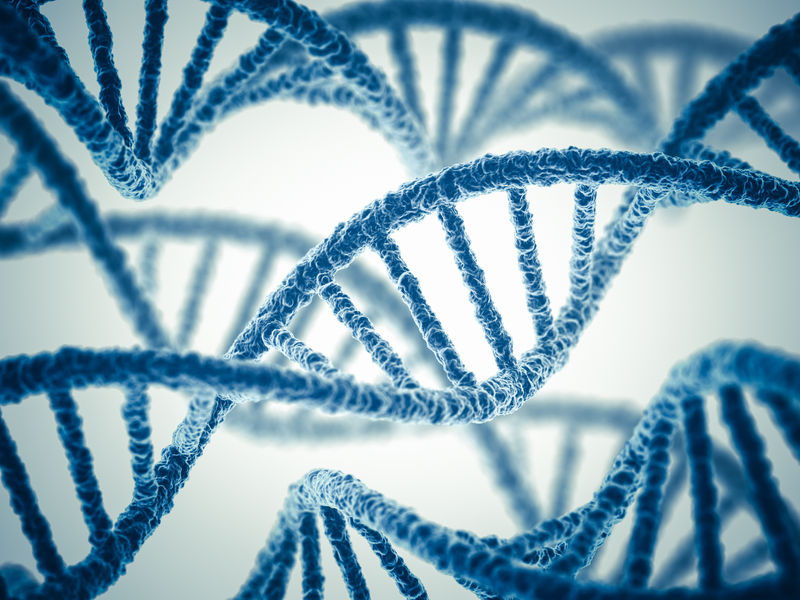
\includegraphics{./figs/DNA-1}
    \caption{\label{fig:fig-DNA-1}DNA}
\end{figure}

\begin{figure}
	\begin{subfigure}{.5\textwidth}
		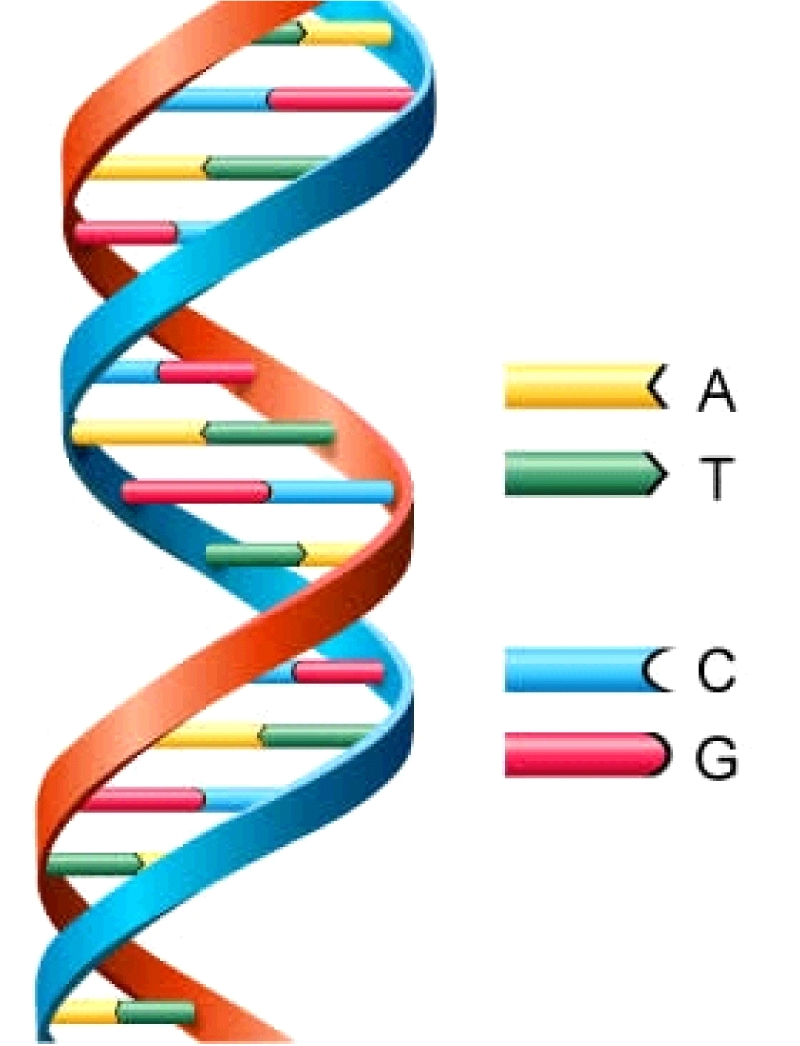
\includegraphics[width=.6\linewidth]{./figs/DNA-2}
	\end{subfigure}
	\begin{subfigure}{.5\textwidth}
		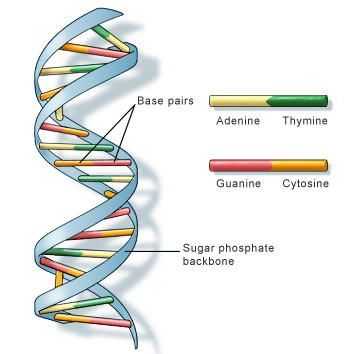
\includegraphics[width=.9\linewidth]{./figs/DNA-3}
	\end{subfigure}
	\caption{\label{fig:fig-DNA-2}DNA scientific analysis}
\end{figure}

An important property of DNA is that it can replicate, or make copies of itself. Each strand of DNA in the double helix can serve as a pattern for duplicating the sequence of bases. This is critical when cells divide because each new cell needs to have an exact copy of the DNA present in the old cell \cite{DNA3}.

\section{DNA Sequencing}
DNA sequence represents a single format onto which a broad range of biological phenomena can be projected for high-throughput data collection \cite{seq1}. 
Over the past years, massively parallel DNA sequencing platforms have become widely available, reducing the cost of DNA sequencing by over two orders of magnitude, and democratizing the field by putting the sequencing capacity of a major genome center in the hands of individual investigators. These new technologies are rapidly evolving, and near-term challenges include the development of robust protocols for generating sequencing libraries, building effective new approaches to data-analysis, and often a rethinking of experimental design (Fig. \ref{fig:fig-NGS-1} and \ref{fig:fig-NGS-2}) \cite{seq2,seq3}.
\begin{figure}
	\centering
	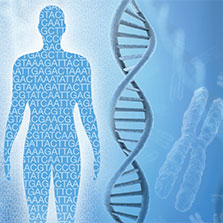
\includegraphics{./figs/NGS-1}
	\caption{\label{fig:fig-NGS-1}DNA sequencing}
\end{figure}

\begin{figure}
	\centerfloat
	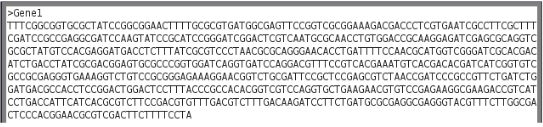
\includegraphics[width=1\linewidth]{./figs/NGS-2}
	\caption{\label{fig:fig-NGS-2}DNA sequencing - Gene example}
\end{figure}

\newpage
One of the core issues of Bioinformatics is dealing with file formats. Some ad hoc simple human readable formats have over time attained the status of de facto standards. A ubiquitous example of this is the ‘FASTA sequence file format’, originally invented by Bill Pearson as an input format for his FASTA suite of tools.
FASTA format is a text-based format for representing either nucleotide sequences, in which nucleotides are represented using single-letter codes. FASTA format allows for sequence names and comments to precede the sequences. As illustrated in Fig. \ref{fig:fig-NGS-5}, the first line in a FASTA file starts either with a ``\textgreater" (greater-than) symbol or, less frequently, a ``;" (semicolon) and was taken as a comment. Subsequent lines starting with a semicolon would be ignored by software. Since the only comment used was the first, it quickly became used to hold a summary description of the sequence, often starting with a unique library accession number, and with time it has become commonplace use to always use ``\textgreater" for the first line and to not use ``;" comments (which would otherwise be ignored) \cite{fasta-fastq1}.
\begin{figure}
	\centerfloat
	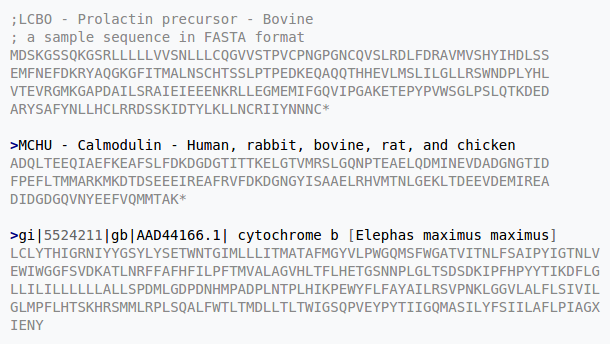
\includegraphics[width=0.8\linewidth]{./figs/NGS-5}
	\caption{\label{fig:fig-NGS-5}FASTA sample sequences}
\end{figure}
Following the initial line (used for a unique description of the sequence) is the actual sequence itself in standard one-letter code. Anything other than a valid code would be ignored (including spaces, tabulators, asterisks, etc...). Originally it was also common to end the sequence with an ``*" (asterisk) character. 
Over time, this format has evolved by consensus; however, in the absence of an explicit standard some parsers will fail to cope with very long ‘\textgreater’ title lines or very long sequences without line wrapping. There is also no standardization for record identifiers.

In the area of DNA sequencing, the FASTQ file format has emerged as another de facto common format for data exchange between tools. It provides a simple extension to the FASTA format: the ability to store a numeric quality score associated with each nucleotide in a sequence (illustrated in Fig. \ref{fig:fig-NGS-6}) \cite{fasta-fastq2}. 
Early FASTQ uses PHRED quality score \cite{fasta-fastq0} (which is a measure of the quality of the identification of the nucleobases generated by automated DNA sequencing where it is logarithmically linked to error probabilities as illustrated below in Fig. \ref{fig:fig-NGS-3} and \ref{fig:fig-NGS-4}). Storing PHRED scores as single characters (or bytes) gave a simple but reasonably space efficient encoding. In order that the file be human readable and easily edited, this restricted the choices to the ASCII printable characters 32–126 (decimal), and since ASCII 32 is the space character, ASCII 33–126 is used instead to encode PHRED qualities from 0 to 93 (i.e. PHRED scores with an ASCII offset of 33).

\begin{figure}
	\centerfloat
	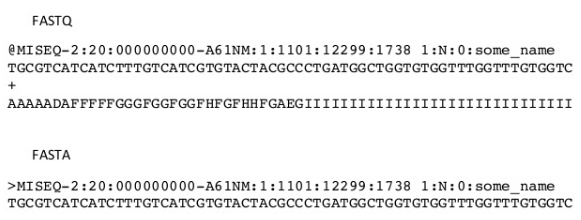
\includegraphics[width=0.9\linewidth]{./figs/NGS-6}
	\caption{\label{fig:fig-NGS-6}FASTQ VS FASTA}
\end{figure}

\begin{figure}
	\centering
	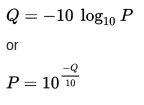
\includegraphics[width=0.4\linewidth]{./figs/NGS-3}
	\caption{\label{fig:fig-NGS-3}Phred quality scores 
	\textit{\textbf{Q}} are defined as a property which is logarithmically related to the base-calling error probabilities \textit{\textbf{P}}}
\end{figure}
\begin{figure}
	\centerfloat
	\includegraphics[width=1\linewidth]{./figs/NGS-4}
	\caption{\label{fig:fig-NGS-4}Phred quality scores are logarithmically linked to error probabilities}
\end{figure}


\section{Next-Generation Sequencing}
As stated above, the field of DNA sequencing technology development has a rich and diverse history. Over the past years, the incentive for developing entirely new strategies for DNA sequencing has emerged on at least four levels, undeniably reinvigorating this field\cite{NGS,NGS1}. First, in the wake of the Human Genome Project, there are few remaining avenues of optimization through which significant reductions in the cost of conventional DNA sequencing can be achieved. Second, the potential utility of short-read sequencing has been tremendously strengthened by the availability of whole genome assemblies for all major model organisms, as these effectively provide a reference against which short reads can be mapped. Third, a growing variety of molecular methods have been developed, whereby a broad range of biological phenomena can be assessed by high-throughput DNA sequencing. And fourth, general progress in technology across disparate fields, including microscopy, surface chemistry, nucleotide biochemistry, polymerase engineering, computation, data storage and others, have made alternative strategies for DNA sequencing increasingly practical to realize. Next-generation DNA sequencing has the potential to dramatically accelerate biological and biomedical research, by enabling the comprehensive analysis of genomes to become inexpensive, routine and widespread, rather than requiring significant production-scale efforts. Since the next-generation sequencing aims to make the vast analysis of genomes less expensive and more spread, it works on enhancing the sequencing time, where too many reads can be generated in a very efficient time. Consequently, it negatively affects the read length and also the sequences accuracy \cite{NGS2}. Actually the next-generation sequencing raises two critical issues, where the first issue is that the read length becomes much shorter than the conventional sequencing, while the second issue is the decrement of the accuracy, where each erroneous nucleotide can be introduced to the read sequence via any of the erroneous actions. There are three erroneous actions listed as; substitution, insertion and deletion illustrated in Fig. \ref{fig:fig-ErrCrr-1}, \ref{fig:fig-ErrCrr-2}, and \ref{fig:fig-ErrCrr-3} respectively. The substitution takes place when the nucleotide is replaced with another erroneous one, while the insertion is when an erroneous nucleotide is newly inserted to the read sequence, and finally the deletion results due to the deletion of a nucleotide from the sequence.

\begin{figure}
	\centerfloat
	\includegraphics[width=1\linewidth]{./figs/ErrCrr-1}
	\caption{\label{fig:fig-ErrCrr-1}{Substitution Error} - \textbf{T} has been erroneously substituted with \underline{A}}
\end{figure}
\vspace{2cm}
\begin{figure}
	\centerfloat
	\includegraphics[width=1\linewidth]{./figs/ErrCrr-2}
	\caption{\label{fig:fig-ErrCrr-2}{Insertion Error} - \underline{G} has been erroneously inserted}
\end{figure}
\vspace{2cm}
\begin{figure}
	\centerfloat
	\includegraphics[width=1\linewidth]{./figs/ErrCrr-3}
	\caption{\label{fig:fig-ErrCrr-3}{Deletion Error} - \underline{T} has been erroneously deleted}
\end{figure}


\section{NGS Sequences Errors Correction}
The reads accuracy is a vital factor in all reads processes that can be applied to the output reads, like genome assemblers \cite{assembly,assembly1}, and genome aligners \cite{alignment}. For example, the assembly of next-generation sequencing reads can not be accomplished successfully until the reads errors are corrected or eliminated. So detecting and correcting (or eliminating) the reads errors is an essential step that should precede the assembly process. This step can be accomplished either by a standalone solution or implicitly within the assembly mechanism. The nucleotide frequency and its quality value are two main factors that are used in evaluating the nucleotide to erroneous or not \cite{ErrCorr,ErrCorr1}. 

\section{Correction Concepts and Definitions}
There are common concepts and definitions used by most of the corrective algorithms. Most of the corrective algorithms generates all the possible sub-sequences (of length k) from a read via a sliding window, which is called \textit{k-mer} (illustrated in Fig. \ref{fig:fig-CrrConcepts-1}); while the term k-mer frequency represents the number of repetition of a k-mer (a specific sub-sequence of length k) in all the reads. Some of the corrective algorithms set a threshold for the k-mer frequency while classifying the k-mer into strong and weak ones. The strong k-mers are those k-mers that are repeated all over the reads x times, where x is greater than the preset threshold; while the weak k-mers are those ones that are repeated y times all over the reads, where y is less than the k-mer frequency threshold. The filtration step that works on classifying the k-mers into strong and weak ones is called ``Spectrum Alignment". The spectrum alignment depends on the k-mers frequencies and/or the nucleotides quality values.
\\
A de Bruijn graph (illustrated in Fig. \ref{fig:fig-CrrConcepts-2}) can be constructed for any sequence, short or long. The first step is to choose a k-mer size, and split the original sequence into its k-mer components. Then a directed graph is constructed by connecting pairs of k-mers with overlaps between the first k-1 nucleotides and the last k-1 nucleotides. The direction of arrow goes from the k-mer, whose last k-1 nucleotides are overlapping, to the k-mer, whose first k-1 nucleotides are overlapping \cite{deBruijn,deBruijn1}.

\vspace{1cm}
\begin{figure}
	\centerfloat
	\includegraphics[width=.3\linewidth]{./figs/CrrConcepts-1}
	\caption{\label{fig:fig-CrrConcepts-1}{K-mer} - All the possible sub-sequences (of length k) from a read}
\end{figure}
\vspace{1cm}
\begin{figure}
	\centerfloat
	\includegraphics[width=1\linewidth]{./figs/CrrConcepts-2}
	\caption{\label{fig:fig-CrrConcepts-2}{De Bruijn Graph} - k-mer of length 7}
\end{figure} 
\newpage
\noindent The number of reads that include a given nucleotide in the sequence is called ``Coverage" \cite{coverage}. The coverage rate of a genome sequences is calculated by the following equation \ref{eq:coverage}
\begin{equation} \label{eq:coverage}
 C = L.N/G 
\end{equation}
where L is the average read length, N is the number of reads and G is the genome length.
\\
Some of the corrective algorithms uses the spectrum alignment in their correction decisions so that the correction takes place by obtaining the nucleotides substitutions that leads to reduce the weak k-mers count by converting them into strong k-mers.
In some other algorithms, the correction takes place using the tree breadth-first search by traversing multi out-going edges nodes, and removing the fewer reads paths, then re-aligning them to the existing path.
\\
There are some corrective algorithms that depend on the reads alignments, where the correction takes place by aligning reads with a common k-mer, then it fixes the misaligned nucleotides based on their occurrences and quality values.
The suffix array also is used in some of the corrective algorithms, where it is built using a string of reads, and the correction takes place with the letter that appears most at each position. Also the suffix trie is used in some other algorithms, where the edges are labelled with DNA letters, while the correction is based on the number of leaves in the sub-trie rooted at the node.
\\
The k-mer hashing table is also used in some corrective algorithms, it is used in storing the total times each nucleotide appears before and after a k-mer, where the error is corrected via the counts. 
\\
Also the k-mer discontinuities is used in some algorithms where the frequencies of adjacent k-mers are calculated and the correction is based on the removal or minimizing the discontinuity.
All of the concepts, stated above, represent the major concepts and paradigms used in the algorithms specialized in correcting the DNA sequencing errors.
\\
The accuracy evaluation of the corrective algorithms depends on calculating some factors as, the true positive rate, the false positive rate, the false negative rate, and the true negative rate. The true positive rate (TP) is the count of the properly corrected nucleotides, while the false positive rate (FP) is the count of the non-erroneous nucleotides that have been wrongly corrected. The false negative rate (FN) is the count of the erroneous nucleotides that haven't been detected as erroneous by the algorithm, while the true negative rate (TN) is the count of the non-erroneous nucleotides that have been properly detected as non-erroneous ones. These four factors are the basics factors that are used in calculating the specificity, sensitivity and the accuracy of the algorithm \cite{analysis}. The specificity rate represents the ability of the algorithm to properly corrects the erroneous nucleotides, and it is calculated by the following equation \ref{eq:sensitivity}:
\begin{equation} \label{eq:sensitivity}
  Sensitivity = TP/(TP+FN) 
\end{equation}
While the sensitivity rate represents its ability to detect the erroneous nucleotides, and it is calculated by the following equation \ref{eq:specificity}: 
\begin{equation} \label{eq:specificity}
  Specificity = TN/(TN+FP) 
\end{equation}
And finally, the accuracy represents the all over error rate, and it is calculated by the following equation \ref{eq:accuracy}:
\begin{equation} \label{eq:accuracy}
  Accuracy = (TP+TN)/(TP+FP+FN+TN)
\end{equation} 
While the gain represents the percentage of errors removed from the data set by the error correction program, and it is calculated by the following equation \ref{eq:gain}:
\begin{equation} \label{eq:gain}
  Gain = (TP-FP)/(TP+FN)
\end{equation} 



\newpage
\chapter{\label{chap:3}Related Work}
This chapter has two major sections, where it shows the different types of NGS errors correction algorithms, and briefly gives an overview for every existent error correction algorithm.
\\
\\
The error correction methodologies can be either an implicit process within the assembly methodology or a standalone solution that reproduces reads after correction. The assemblers that have embedded error correction are Euler \cite{Euler}, Velvet \cite{Velvet}, AllPaths \cite{AllPaths} and SOAP \cite{Soap}. While the standalone methodologies are Coral \cite{Coral}, Quake \cite{Quake}, Reptile \cite{Reptile}, HSHREC \cite{HShrec}, HiTEC \cite{HiTec}, RACER \cite{Racer}, Pollux \cite{Pollux}, Parallel Error Correction with CUDA \cite{Cuda}, and Error Corrector (EC) \cite{EC}.
\section{Substitution Only Corrective Algorithms}
They are algorithms that are able to correct only the substitution DNA reads errors, these algorithms are: Euler \cite{Euler}, Velvet \cite{Velvet}, AllPaths \cite{AllPaths}, SOAP \cite{Soap}, Quake \cite{Quake}, Reptile \cite{Reptile}, HiTEC \cite{HiTec}, RACER \cite{Racer}, Parallel Error Correction with CUDA \cite{Cuda}, and Error Corrector (EC) \cite{EC}. Check Fig. \ref{fig:fig-RW-1}.
\subsection{Euler}
Euler \cite{Euler} assembly method runs a filtration step called spectrum alignment that aims to classify the k-mers into two categories according to their frequencies all over the reads. Strong k-mers are the ones with high frequencies, while weak k-mers are the ones with lower frequencies. The correction takes place by executing a greedy exploration for base call substitutions aiming to reduce the weak k-mers count.
\\
Since in de novo genome sequencing the sampled genome is not known, EULER uses the number of times a k-mer appears to determine if it is in Gk(the set of k-mers in a genome G), where a threshold M determines whether a k-mer is a solid or a weak one. The read that contains all solid k-mers is referred to as a solid read. Hence, the goal of EULER is to correct the reads so that they are all solid reads.
\\
And the set of all k-mers is updated after each iteration of corrections, so that the reads are deleted if they are not able to be corrected after the last iteration. After that, the assembly of the genome begins after the error correction.
\\
The datasets with low coverage require that the threshold M to be set with a low value so that valid k-mers are not considered weak, but this will cause correct reads to be considered incorrect. 
Where increasing the length of k, will help in reducing the false positive rate and increasing the difficulty of determining the correction changes.
\\
Also in Euler, the reads with erroneous ends are trimmed, because the ends of reads tend to have more errors than the rest of the read, so it's difficult to determine the correct changes to the ends of reads.

\subsection{Velvet}
Velvet's \cite{Velvet} works by efficiently manipulating de Bruijn graphs through simplification and compression, without the loss of graph information, by converging non-intersecting paths into single nodes, i.e. it merges nodes that do not affect the path generated in the graph, so that, whenever a node A has only one outgoing arc that points to node B, with only one ingoing arc, the nodes can be merged.
\\
Velvet eliminates errors and resolves repeats by first using an error correction algorithm that merges sequences together. Repeats are then removed from the sequence via the repeat solver that separates paths which share local overlaps.
\\
\\
In other words, velvet's tour bus algorithm uses breadth-first search (BFS), starting at nodes with multiple out-going edges, where candidate paths are traversed in step, moving ahead one node on all paths per iteration, until the path lengths exceed a threshold. Velvet removes the path representing fewer reads then re-aligns reads from the removed path to the remaining path.

\subsection{AllPaths}
AllPaths \cite{AllPaths} uses a read-correcting preprocessor related to the spectral alignment in Euler, where the reads filtration is based on quality values, which is further used in correcting some substitutional errors. 

\subsection{SOAP}
SOAP \cite{Soap} filters and corrects reads using pre-set thresholds for k-mer frequencies. It removes bubbles with an algorithm like Velvet's tour bus, with higher read coverage determining the surviving path (read).

\subsection{Quake}
Quality-aware Detection and Correction of Sequencing Errors (Quake) \cite{Quake} determines a cut-off value which separates trusted k-mers from untrusted k-mers, using the distribution of k-mers based on their quality scores. The intersection of the untrusted k-mers is used to localize the search for an error in a read. Quake tries to evaluate the conditional probability of assigning the actual nucleotides of the sequenced fragment, given the observed nucleotides.
\\
It relies on k-mer coverage and quality scores to correct reads, as it uses a method of evaluating the quality of a k-mer based on the associated quality scores for each base. 
\\
The k-mers weighing is based on quality scores, where the low coverage true k-mers will have high quality scores and the high coverage k-mers with errors will have low quality scores.
\\
Quake begins by counting all the k-mers in the dataset, so the value of k, has a significant impact on the performance of Quake. But actually for an appropriate choice for k, Quake uses the following equation \ref{eq:quake-k} to set k (where G is the size of the genome).
\begin{equation} \label{eq:quake-k}
 k \approx log_{4} 200G  
\end{equation}
After that, it determines a cut-off value which separates trusted k-mers from untrusted k-mers, using the distribution of k-mers based on their quality values, where the reads with untrusted k-mers are considered for correction, and the errors are detected based on the intersection of the untrusted k-mers, which is used to localize the search for an error in a read. 
\\
Actually, Quake considers every base covered by the right most trusted k-mer, and left most trusted k-mers to be correct, so if the errors are near the end of a read, it will be checked first whether it is in the right most or left most, after that the decision will be taken. Also it tries to evaluate the conditional probability of a assigning the actual nucleotides of the sequenced fragment, given the observed nucleotides.
\\
\\
Quake has some heuristics, like ambiguous true correction, where the repeats imply to having multiple sets of valid corrections, with a small difference in the likelihood of each correction, so a true correction is ambiguous. So, it continues past the threshold to ensure that another valid set does not exist. 
\\
Quake stops correcting if the region is filled with low quality scores, where the reads with a region containing $\geq$ 13 positions with a probability of error $>$ 1\% are not corrected. And the reads with regions containing $\geq$ 9 positions with a probability of error $>$ 1\%, the likelihood ratio threshold is increased to $10^{-3}$.
\subsection{Reptile}
Representative Tiling for Short Read Error Correction (Reptile) \cite{Reptile} uses the spectral alignment approach used in Euler, with the quality score information if available. Trying to create approximate multiple alignments by considering all reads with pairwise hamming distance less than a pre-set threshold. 
\\
\\
Reptile considers all reads with pairwise Hamming distance less than a set threshold, where it finds the multiple alignments by only aligning k-mers in the reads. Actually, it chooses the size of k so that the expected number of occurrences of any k-mer in the genome should not exceed one. And it uses contextual information to help resolve errors without increasing k.
\\
\\
The main disadvantage of Reptile is that the user should set the parameters, so it
requires running scripts and analyzing the results to obtain the proper parameters.

\subsection{HiTEC}
High Throughput Error Correction (HiTEC) \cite{HiTec} uses a suffix array that is built using a string of reads and their reverse complements. The correction of an erroneous nucleotide takes place with the letter that appears most at that position.
\\
\\
HiTec uses the suffix array as it is a more time and space efficient data structure than the suffix trie, where it uses an array that stores the length of the longest common prefix (LCP) between consecutive suffixes in the suffix array.
\\
\\
Actually, it assumes that the length of the genome and the error rate of the dataset is supplied. Also HiTEC assumes that a read, starting at position j of the genome, contains an error in position m and that the previous w positions, $r_{i} [m - w..m - 1]$, are correct.
\\
As the length of witness length (w) decreases:

\begin{itemize}
	\item The number of uncorrectable reads U(w) decreases.
	\item The probability of seeing the witness increases, so the correct positions changed incorrectly. 
	\item The number of destructible reads D(w) increases.
	\item A value for w must be found that minimizes U(w)+ D(w). 
\end{itemize}

So, HiTEC uses a variation of witness lengths based on the optimal witness length to achieve high accuracy.
\\
\\
After that, HiTEC uses the majority of one base at a position, the erroneous base is changed to the base that appears most at that position. If there is no ambiguity in the correct letter then the correction is made. But, if there is ambiguity, then the next two letters are checked in order to decide how to correct the read. And finally, it stops correcting when the number of bases changed during one iteration is less than 0.01\% of the total number of bases, or after nine iterations or corrections.
\\
\\
HiTEC only requires modest coverage to make corrections. So, the datasets with high coverage are split into several sets with lower coverage that are independently corrected. 
\\
\\
The disadvantages of HiTEC can be listed as:
\begin{itemize}
	\item It does not correct reads with ambiguous letters.
	\item It can only correct datasets if the reads are all the same length.
	\item It does not run in parallel mode.
\end{itemize}

\subsection{RACER}
Rapid and Accurate Correction of Errors in Reads (RACER) \cite{Racer} is able to correct datasets that have varying read lengths. Using a hash table that stores the total number of times each nucleotide appears before and after each k-mer, where the error is corrected via the counts.
\\
\\
Actually, RACER replaces the suffix array approached used in HiTEC with a more time and space efficient hash table. And as stated above, this hash table stores the k-mers in each read, and the total times each base appears before and after each k-mer. While, the optimal k-mer length is calculated with a similar statistical analysis as HiTEC, i.e, it's value must be found that minimizes U + D, where U is the number of uncorrectable reads and D is the number of destructible reads. In other words, it choose k that will minimize the number of false positives and maximize the number of corrections. And after the k-mers and the counters have been calculated, the reads are corrected based on the counts.
\\
\\
RACER encodes the input sequences using two bits to represent each base, where the k-mer and its reverse complement must be searched, and only the one with the smaller encoding key is stored. Consequently, it shows a great enhancement in time and memory usage, where there is no algorithm can beat RACER in time.
\\
One more significant advantage of RACER is that it is able to correct datasets that have varying read lengths, and runs in both serial and parallel mode.
 

\subsection{Parallel Error Correction with CUDA}
Parallel Error Correction with Compute Unified Device Architecture (CUDA) \cite{Cuda} uses the spectrum alignment besides a voting algorithm for the single-mutation using each letter, hence errors can be fixed based on high values in the voting matrix.
\\
\\
CUDA (Compute Unified Device Architecture) is an extension of C/C++ to write scalable multi-threaded programs for CUDA-enabled GPUs, where CUDA programs can be executed on GPUs with NVIDIA’s Tesla unified computing architecture, while CUDA programs contain a sequential part, called a kernel.
\\
\\
CUDA uses the single-mutation voting algorithm, where it firstly initialize the voting matrix by zeros for each of (A, C, T, G) for every nucleotide, and loop on every read to check whether it is in the spectrum or not. If it is found that the read is not in the spectrum, it loops on every nucleotide against its voting matrix and increase the vote by 1 for every successful replacement (that makes the reads fit into the spectrum). After that, the errors can be fixed based on high values in the voting matrix.
\subsection{Error Corrector}
Error Corrector (EC) \cite{EC} an error correction algorithm for correcting short reads with substitution errors only. Using k-mers hashing tables to find the neighbours of each of the reads, where each read is corrected using its neighbours.
\\
\\
In other words, the steps of Error Corrector (EC) can be broken into three independent tasks. At first it builds k-mers and hashes the k-mers into hash tables. After that, by using these hash tables it finds the neighbours of each of the reads. And finally, each read is then corrected using the neighbours of the read.

\begin{figure}
	\centerfloat
	\includegraphics[width=1.35\linewidth]{./figs/RW-1}
	\caption{\label{fig:fig-RW-1}An illustrative summary for the substitution only corrective algorithms}
\end{figure}


\section{Substitution, Insertion And Deletion Corrective Algorithms}
They are algorithms that are able to correct all types of DNA reads errors, these algorithms are: Coral \cite{Coral}, HSHREC \cite{HShrec}, and Pollux \cite{Pollux}. Check Fig. \ref{fig:fig-RW-2}

\subsection{Coral}
Correction with Alignments (Coral) \cite{Coral} is able to correct all types of errors (substitution, insertion and deletion). The methodology is built on scoring the alignments between short reads, where each alignment runs on a base read with all the reads that have at least one common k-mer with this base read. Then the correction takes place for the misaligned positions depending on the number of times each letter occurs in addition to quality scores of the nucleotide.
\\
Coral uses multiple sequence alignments (MSA) \cite{coral-alignment} between short reads to detect errors, where it calculates the gap penalty and mismatch penalty (parameters for scoring the alignments) have a significant impact on the quality of the corrections. 
\\
The main defect in Coral is that it isn't able to correct mixed datasets that contain both substitution errors with insertion and deletions ones.
For substitution errors, Coral sets the gap penalty with a very high value to prevent insertions and deletions in the alignments. While for insertion and deletion errors, Coral sets the gap and mismatch penalties to be equal.
\\
Coral can summarize the algorithm as:
\begin{enumerate}
	\item Indexing Reads, where a hash table is used to store the k-mers and the reads that contain each k-mer. And in order to save space, Coral store the information of only the lexicographically smaller of the k-mer \& its reverse. It also does not store any k-mers that contain ambiguous letters.
	\item Multiple Alignments, where Coral starts each alignment with one read which is called the base read, and all the reads that share at least one k-mer with the base read are found using the k-mer hash table, and they are called neighbourhood of the base. If the neighbourhood of the base read is very large or very small, then Coral does not perform any alignments.
 As, if it's very large, then the reads likely came from different regions in the genome and the MSA will take a long time to compute, as the alignments will be very poor. But, if it's very small, then there is likely not enough coverage to make any significant corrections.
\\
Coral doesn't correct the reads that have been corrected before. So, if a read has already been corrected in a previous alignment, Coral tries to align it to the consensus without errors in the region of the k-mer. And, if a read aligns perfectly to the consensus then the rest of the read is not aligned to save time. But, if a read has many errors compared to the consensus then it stops aligning the read and moves on to the next one. And if the gaps are not allowed then a gap-less alignment is performed between a read and the consensus sequence.

\item Correcting Reads, where Coral calculates the number of misaligned positions for each read compared to the consensus sequence. And if the quality of the alignment is above a preset threshold, then it will be used to correct the aligned reads. The support threshold for each position in the consensus sequence is calculated as: (num of times each letter occurs)/ (total num of reads aligned at that position). In case a read differs from the consensus at any position, then the letter is changed in the read provided the support is above the threshold. And if quality scores are available and there is a gap in an aligned read, then:
 quality score of the gap = avg (the quality scores of the bases flanking the gap).
\end{enumerate}
The complexity of Coral is illustrated as follow (assuming that where M is the combined total length of the reads, L is the maximum number of reads in a neighbourhood, and r is the longest read length):
\begin{itemize}
	\item If gaps are allowed, the worst case runtime is O(MrL).
	\item If only mismatches are allowed, the worst case runtime is O(ML).
	\item The space for the hash table that stores the k-mers is bounded by O(M).
	\item The space complexity for computing the MSA is O(Lr + r\textsuperscript{2}).
	\item The overall space complexity is O(M).
\end{itemize}

\subsection{HSHREC}
Hybrid Short Read Error Correction (HSHREC) \cite{HShrec} is able to correct all types of errors (substitution, insertion and deletion). The methodology depends on the alignment of a read with others using a suffix trie, where the edges are labelled with DNA letters and a node weight is the number of leaves in the sub-trie rooted at that node. On the down levels, a node with more than one child is considered to have a substitution error, while extra branching in the generalized suffix trie is caused by insertion and deletion erroneous actions.
\\
\\
SHREC was designed to correct substitution errors, and HSHREC is able to correct both substitution errors and insertion and deletion erroneous actions.
\\
HSHREC assumes that the input contains k reads randomly sampled from a genome with read length n, where n can vary in length. The errors are detected in a read by aligning it to the other reads using a suffix trie, where the erroneous region of the read has a low weight in the trie and this is the area that will be corrected.
\\
\\
HSHREC resolves the ambiguity that can be caused by single nucleotide polymorphisms (SNPs). The single nucleotide polymorphisms (SNPs) is the phenomena of changing single nucleotide that differ between individuals of the same species, and they can appear as errors. Actually, SNPs are the most abundant type of genetic marker and their high density makes them ideal for studying the inheritance of genomic regions \cite{SNP1,SNP2}, so its discovery and genotyping are essential to genetic mapping. There remains a need for a simple, inexpensive platform that allows high-density SNP discovery and genotyping in large populations \cite{SNP3}. But HSHREC analyse it as: since the errors at the SNP location will only be in a few reads, and SNPs will be present in several reads, it is possible to differentiate them.
\\
\\
In HSREC, each read has a unique suffix by concatenating a unique number from 1 to 2k to the end of each string in R (the set of reads, and their reverse complements). And the edges of the trie are labeled with DNA letters, and an ambiguous letter N, where the concatenation of edge labels from the root to a node is called a path-label. 
\\
For any suffix of a string in R, there is a path-label that contains that suffix. And the weight of a node in the trie is the number of leaves in the subtrie that is rooted at that node, and is the number of suffixes in that subtrie. 
\\
The level of a node is the length of the path from the root to the node. In the top levels of the trie almost all nodes have four or five children. while in the down levels of the trie almost all nodes have only one child. So, if a child at down levels has more than one child then it is likely an error, and the node with the lower weight is likely the erroneous base. 
\\
So, HSHREC algorithm traverses the trie to identify errors at the intermediate levels of the trie. And it tries to correct each error with a substitution, and the remaining errors are treated as insertions or deletions.
\\
In SHREC, it compares the subtrie rooted at the low weight node to the subtries rooted at the siblings of the node, while the insertion and deletion erroneous actions cause extra branching in the generalized suffix trie. The insertion erroneous action creates a low weight node, so the deletion corrective action of the node causes the children rooted at the node and their siblings to be merged. And a comparison of the subtries before and after the deletion determine if the deletion is a proper way to correct the node or not. 

\subsection{Pollux}
Platform Independent Error Correction of Single and Mixed Genomes (Pollux) \cite{Pollux} calculates the k-mer frequencies in the entire set of reads. Identifying the discontinuities by comparing the frequencies of adjacent k-mers within reads, assuming that individual k-mers are not erroneous. The discontinuities within reads are used to find error locations and evaluate correctness. The correction is chosen to be the one that removes or minimizes the k-mer count discontinuity.
\\
\\
Pollux decomposes each read into k-mers and then calculates the k-mer frequencies in the entire set of reads. The nucleotide is represented with a two-bit alphabet and a hash-table strategy is used to help in using large k-mers (with length 31) to avoid common short repeats which might otherwise confound the correction procedure.
\\
\\
Firstly it identifies the individual k-mers as not erroneous, then identifies the discontinuities by comparing the frequencies of adjacent k-mers within reads. The discontinuities within reads are used to find error locations and evaluate correctness. A read that is not erroneous is assumed to have a k-mer count profile that is reflective of a random sampling process, given local coverage. In contrast, a read that contains an error is likely to have k-mer counts that deviate unexpectedly from this random process. Evaluating multiple k-mers containing bases following the erroneous base to ensure our correction is appropriate. The correction is chosen to be the one that removes or minimizes the k-mer count discontinuity. If there exist multiple corrections which achieve this, the correction is chosen to be the one that improves the most k-mer counts maximally beyond the current erroneous location. Pollux corrects each read independently and does not update recorded k-mer counts as a result of correction.
 
\begin{figure}
	\centerfloat
	\includegraphics[width=1.35\linewidth]{./figs/RW-2}
	\caption{\label{fig:fig-RW-2}An illustrative summary for the substitution, insertion and deletion corrective algorithms}
\end{figure}

\newpage
\chapter{\label{chap:4}K-mer Grouping Error Correction Algorithm}
This chapter illustrates the working methodology of K-mer Grouping Error Correction (KGEC - the first proposed algorithm) in details, where the pseudo code, diagram and examples are discussed in details. While the evaluation will be discussed in chapter \ref{chap:6}.
\\
\\
The first proposed algorithm (Kmer Grouping for Error Correction or KGEC) aims to correct all types of errors and to boost the next-generation sequencing output accuracy. It tries to compete in the accomplishment time with the currently existent algorithms specialized in correcting all types of the errors found in the output of the next-generation sequencing, i.e. the substitution erroneous actions, the insertion erroneous actions and the deletion erroneous actions). Also it has the flexibility to run more than a correction iteration, which usually helps in enhancing the accuracy.
\section{\label{sec:alg1-meth}Methodology}
As stated before, this algorithm aims to correct all types of errors (substitution, insertion and deletion). It mainly depends on k-mers grouping. So, firstly it builds a hash table that maps the k-mer into integer and saves its frequency all over the reads. The hashing algorithm (illustrated in Fig. \ref{fig:fig-KGEC-HASH}) is inherited from Coral \cite{Coral}, where the k-mer and its complement will map to the same integer, where the k-mer length is chosen by experiment for each dataset to be the one that gives the highest accuracy. Then, it groups k-mer based on having same nucleotides in the same order, with a mutation in the first, middle and last positions (so the k-mer length is chosen to be an odd number starting from five and maximumly equals to half the read length so that the mutations will cover all of the reads nucleotides). After that, each k-mer group will search for the k-mer with the highest frequency to use it in unifying all of the rest of the group members (k-mers) to make them all have the same nucleotides in the same order of the k-mer with the highest frequency. In case of having more than a k-mer having the same highest frequency within the same group, the algorithm searches for the one with the highest frequency and highest quality value average of its nucleotides, where the quality value of the nucleotide in the k-mer is calculated as the average of the quality value of this nucleotide in the reads that have this k-mer as a subsequence. 
\\
\\
After correcting the k-mer groups with their best k-mer, it checks those k-mers that does not belong to any group and consequently is not corrected yet, and tries to re-group them again but this time based on having same nucleotides in the same order, with a mutation in the three positions of the nucleotides that have lowest three quality values compared to the rest of the nucleotides within the same k-mer. And similarly, each k-mer group will search for the k-mer with the highest frequency to use it in unifying all of the rest of the group members (k-mers) to make them all have the same nucleotides in the same order of the k-mer with the highest frequency (and highest quality value average if needed). 
\\
Check the illustrative example shown in Fig. \ref{fig:fig-KGEC-EX} and the diagram shown below in Fig. \ref{fig:fig-First-Proposal-1}. Also the pseudo-code of the hashing algorithm and that of the correction are illustrated in Fig. \ref{fig:fig-KGEC-HASH} and Fig. \ref{fig:fig-KGEC-ALG} respectively.
\\
\\
Finally, the algorithm corrects the reads with corrected k-mers, where it decides the corrective action (substitution, insertion and deletion) based on studying the erroneous nucleotide and its neighbours (similarly to H-RACER \cite{HRACER} correction action procedure, so it will be explained in details in the following chapter). After this step, it will repeat the flow again if it was running in iterative mode (set by a given parameter that sets the iterations count).

\begin{figure}
\vspace{0cm}
\begin{bordered}
\begin{enumerate}
	\item \underline{Extracted K-mers with Frequencies}
	\begin{enumerate}
		\item CCGTAAT - Freq. = 9
		\item CGCTACT - Freq. = 13
		\item GTACGGT - Freq. = 8
		\item AGCTACT - Freq. = 4
		\item GTCCTGT - Freq. = 3
		\item ACGTAAT - Freq. = 2
		\item GGCCACT - Freq. = 2
		\item GGCCTAA - Freq. = 1
		\item TGCCACC - Freq. = 3
	\end{enumerate}
	\item \underline{K-mers Grouping (\textit{0, (k-1)/2, k})}
	  \begin{enumerate}
		\item \underline{CCGTAAT} \hspace{1.8ex}- Freq. = 9
		\item \textbf{CGCTACT} - Freq. = 13
		\item GTACGGT \hspace{1.8ex}- Freq. = 8
		\item \textbf{AGCTACT} - Freq. = 4
		\item GTCCTGT \hspace{1.8ex}- Freq. = 3
		\item \underline{ACGTAAT} \hspace{1.8ex}- Freq. = 2
		\item \textbf{GGCCACT} - Freq. = 2
		\item GGCCTAA \hspace{1.8ex}- Freq. = 1
		\item \textbf{TGCCACC} - Freq. = 3
	  \end{enumerate}
	  Hence, there are two groups formed:
	\begin{itemize}
	  \item 
	  \begin{enumerate}
		\item \underline{C}\textbf{CG}\underline{T}\textbf{AA}\underline{T} - Freq. = 9
		\item \underline{A}\textbf{CG}\underline{T}\textbf{AA}\underline{T} - Freq. = 2
	  \end{enumerate}
	\end{itemize}
	\begin{itemize}
	  \item 
	  \begin{enumerate}
		\item \underline{C}\textbf{GC}\underline{T}\textbf{AC}\underline{T} - Freq. = 13
		\item \underline{A}\textbf{GC}\underline{T}\textbf{AC}\underline{T} - Freq. = 4
		\item \underline{G}\textbf{GC}\underline{C}\textbf{AC}\underline{T} - Freq. = 2
		\item \underline{T}\textbf{GC}\underline{C}\textbf{AC}\underline{C} - Freq. = 3
	  \end{enumerate}
	\end{itemize}
	While the remaining with no group are:
	\begin{itemize}
		\item GTACGGT - Freq. = 8
		\item GTCCTGT - Freq. = 3
		\item GGCCTAA - Freq. = 1
	\end{itemize}
	\item \underline{Correcting K-mer Groups}
     \begin{itemize}
	  \item Corrective: \underline{C}\textbf{CG}\underline{T}\textbf{AA}\underline{T} - \textbf{Freq. = 9}
	  \begin{enumerate}
		\item \underline{A}\textbf{CG}\underline{T}\textbf{AA}\underline{T} - Freq. = 2
	  \end{enumerate}
	\end{itemize}
	\begin{itemize}
	  \item Corrective: \underline{C}\textbf{GC}\underline{T}\textbf{AC}\underline{T} - \textbf{Freq. = 13}
	  \begin{enumerate}
		\item \underline{A}\textbf{GC}\underline{T}\textbf{AC}\underline{T} - Freq. = 4
		\item \underline{G}\textbf{GC}\underline{C}\textbf{AC}\underline{T} - Freq. = 2
		\item \underline{T}\textbf{GC}\underline{C}\textbf{AC}\underline{C} - Freq. = 3
	  \end{enumerate}
	\end{itemize}
	\item \underline{K-mers (\textit{weakest 3 nucleotides})}
	\begin{itemize}
		\item 
	Hence, one group is formed \textit{assuming weakest 3 nucleotides of GTACGGT are the three middles}
		\begin{enumerate}
		\item GT\underline{A}\underline{C}\underline{G}GT - \textbf{Freq. = 8}
		\item GT\underline{C}\underline{C}\underline{T}GT - Freq. = 3
		\end{enumerate}
	\end{itemize}
	\item \underline{Correcting K-mers Groups}
	\begin{itemize}
		\item GT\underline{A}\underline{C}\underline{G}GT - \textbf{Freq. = 8}
		\begin{enumerate}
		\item GT\underline{C}\underline{C}\underline{T}GT - Freq. = 3
		\end{enumerate}
	\end{itemize}
\end{enumerate}
\end{bordered}
\caption{\label{fig:fig-KGEC-EX}KGEC Grouping and Correction Decision Examples}
\end{figure}

\begin{figure}
	\centerfloat
	\includegraphics[width=1.6\linewidth]{./figs/First-Proposal-1}
	\caption{\label{fig:fig-First-Proposal-1}KGEC Diagram}
\end{figure}

\begin{figure}
\vspace{0.1cm}
\begin{bordered}
Assume a read represented as: $r=s_1s_2\cdots s_n$
\\
Assume k represents the k-mer length
\\
Set code\_a with 0x00
\\
Set code\_c with 0x01
\\
Set code\_g with 0x02
\\
Set code\_t with 0x03
\\
Set gram as uint64\_t with zero value (represents the k-mer)
\\
Set gram\_reverse as uint64\_t with zero value (represents the reverse of k-mer)
\\
Set mask as uint64\_t with ((uint64\_t) 1 $<<$ (2 * k)) - 1 (used in k-mer masking)
\\
Set pre\_gram as uint64\_t with zero value (used in k-mer hashing check)
\\
Set pre\_mask as uint64\_t with zero value (used in k-mer hashing check)
\\
\\
For every nucleotide $s_i$ in $r$ 
\begin{enumerate}
\addtolength{\itemindent}{1cm} 
\item Check the value of $s_i$: 
\vspace{-2mm}
\begin{enumerate}
\addtolength{\itemindent}{1cm}

	\item if $s_i$ equals `A' or `a'
	
	\noindent\hspace{1cm}then,
	
	\begin{itemize}
    \addtolength{\itemindent}{1cm}
	  \item Reset gram with: gram $<<$ 2 $|$ code\_a
      \item Reset gram\_reverse with: gram\_reverse $>>$ 2 $|$ code\_t $<<$(k - 1)*2
	\end{itemize}
	
	\item if $s_i$ equals `C' or `c'
	
	\noindent\hspace{1cm}then,

	\begin{itemize}
    \addtolength{\itemindent}{1cm}
	  \item Reset gram with: gram $<<$ 2 $|$ code\_c
	  \item Reset gram\_reverse with: gram\_reverse $>>$ 2 $|$ code\_g $<<$(k - 1)*2
	\end{itemize}
	
	\item if $s_i$ equals `G' or `g'
	
	\noindent\hspace{1cm}then,

	\begin{itemize}
    \addtolength{\itemindent}{1cm}	
     	\item Reset gram with: gram $<<$ 2 $|$ code\_g
      	\item Reset gram\_reverse with: gram\_reverse $>>$ 2 $|$ code\_c $<<$(k - 1)*2
	\end{itemize}
	
	\item if $s_i$ equals `T' or `t'
	
	\noindent\hspace{1cm}then,

	\begin{itemize}
    \addtolength{\itemindent}{1cm}
      \item Reset gram with: gram $<<$ 2 $|$ code\_t
	  \item Reset gram\_reverse with: gram\_reverse $>>$ 2 $|$ code\_a $<<$(k - 1)*2
	\end{itemize}

\end{enumerate}

\item Reset gram with: gram \& mask

\item Reset gram\_reverse with: gram\_reverse \& mask;

\item Check if $i >$ k, then, check:
\vspace{-2mm}
\begin{enumerate}
\addtolength{\itemindent}{1cm}
      \item if gram $<$ gram\_reverse \&\& (gram \& pre\_mask) == pre\_gram
      	
      \noindent\hspace{1cm}then, add a k-mer to the hash array at index mapped to gram
	   
	  \item if gram\_reverse $<$ gram \&\& (gram\_reverse \& pre\_mask) == pre\_gram
	  
      \noindent\hspace{1cm}then, add a k-mer to the hash array at index mapped to gram\_reverse
	  
\end{enumerate}            
End For	
\end{enumerate}
\end{bordered}
\caption{\label{fig:fig-KGEC-HASH}KGEC K-mer Hashing Abstraction}
\end{figure}

\begin{figure}
\vspace{0.1cm}
\begin{bordered}
Assume kmer\_hash\_arr is an array that hold the hashing table with size m
\\
Assume k represents the k-mer length
\\
\\
For every k-mer in kmer\_hash\_arr

\noindent\hspace{0.4cm} Check if this k-mer doesn't belong to any k-mer group

\noindent\hspace{0.4cm} then,

\vspace{-3mm}
\begin{enumerate}
\addtolength{\itemindent}{1cm}
	  \item Initialize a new k-mer group

	  \item Add this k-mer to the new k-mer group

      \item Generate all k-mers having typical nucleotides as this k-mer, except,
      
      \noindent\hspace{1cm} for these positions \{0, (k-1)/2, k-1\}, it may have different nucleotide
      
      \item For every generated k-mer
	
		\noindent\hspace{1.4cm} if the hash of this generated k-mer exists in kmer\_hash\_arr 
		
		\noindent\hspace{1.4cm} then, add this generated k-mer to the new k-mer group created above
		
		\noindent\hspace{1.4cm} else, do nothing
		
		\noindent\hspace{1cm} End For
		
\end{enumerate}            
\vspace{-3mm}

End For
\\
\\
For every k-mer group 

\vspace{-3mm}
\begin{enumerate}
\addtolength{\itemindent}{1cm}
  \item Search for the k-mer with the highest frequency 

  \item Check if there are more than one k-mer having the highest frequency

  \noindent\hspace{1cm} then, set corrective\_kmer as the one with the highest frequency and quality

  \noindent\hspace{1cm} else, set corrective\_kmer as the one with the highest frequency

  \item For every k-mer in this k-mer group

  \noindent\hspace{1.4cm}Mark this k-mer's nucleotides at \{0, (k-1)/2, k-1\} to be corrected 
  
  \noindent\hspace{1.4cm}with their corresponding one in the corrective\_kmer
  
  \noindent\hspace{1cm} End For
\end{enumerate}            
\vspace{-3mm}

End For
\\
\\
For every k-mer in kmer\_hash\_arr

\noindent\hspace{0.4cm} Check if this k-mer doesn't belong to any k-mer group

\noindent\hspace{0.4cm} then,

\vspace{-2mm}
\begin{enumerate}
\addtolength{\itemindent}{1cm}
	  \item Set weak\_positions array to hold the position of the three nucleotides with 
	  
	  \noindent\hspace{1cm}the lowest quality
	  
	  \item Initialize a new k-mer group

	  \item Add the weak\_positions element to the new k-mer group

	  \item Add this k-mer to the new k-mer group

      \item Generate all k-mers having typical nucleotides as this k-mer, except,
      
      \noindent\hspace{1cm} for the positions in weak\_positions, it may have different nucleotide
      
      \item For every generated k-mer
	
		\noindent\hspace{1.4cm} if the hash of this generated k-mer existent in kmer\_hash\_arr 
		
		\noindent\hspace{1.4cm} then, add this generated k-mer to the new k-mer group created above
		
		\noindent\hspace{1cm} End For

\end{enumerate}            
\vspace{-3mm}
End For
\\
\\
For every k-mer group 
\vspace{-3mm}
\begin{enumerate}
\addtolength{\itemindent}{1cm}
  \item Search for the k-mer with the highest frequency 

  \item Check if there are more than one k-mer having the highest frequency

  \noindent\hspace{1cm} then, set corrective\_kmer as the one with the highest frequency and quality

  \noindent\hspace{1cm} else, set corrective\_kmer as the one with the highest frequency

  \item For every k-mer in this k-mer group

  \noindent\hspace{1.4cm}Mark this k-mer's nucleotides at the weak\_positions element of this    
  
  \noindent\hspace{1.4cm}k-mer group to be corrected with their corresponding one in the 
  
  \noindent\hspace{1.4cm}corrective\_kmer
  
  \noindent\hspace{1cm} End For
\end{enumerate}            
\vspace{-3mm}
End For		
\end{bordered}
\caption{\label{fig:fig-KGEC-ALG}KGEC Grouping and Correction Decision Pseudo-Code - O(\textit{$4^m$})}
\end{figure}


\chapter{\label{chap:5}H-RACER Algorithm}
This chapter illustrates the working methodology of H-RACER (the second proposed algorithm) in details, where the pseudo code, flowchart and examples are discussed in details. While the evaluation will be discussed in chapter \ref{chap:6}.
\\
\\
The second proposed algorithm (Hybrid RACER or H-RACER) \cite{HRACER} is the newly proposed algorithm that aims to correct all types of errors. H-RACER follows the same algorithm of RACER in detecting errors and deciding their corrections, the newly added part in H-RACER is the detection of the error type in order to apply the correction properly for datasets with varying error types.

\section{Methodology}
As stated before, H-RACER \cite{HRACER} aims to correct all types of errors (substitution, insertion, and deletion). Although RACER is the fastest DNA error correction algorithm existent nowadays with a high accuracy, but it can not correct all types of errors, it can only correct substitutions. So, H-RACER is proposed in order to correct all types of errors. Hence, it follows the same algorithm of RACER in detecting errors and deciding their corrections, and the newly added part is the detection of the error type in order to apply the correction properly for datasets with varying error types.
\\
\\
H-RACER detects the error type for an erroneous nucleotide by studying its correction value (obtained by RACER) against its neighbours, then decides the corrective action (substitute, insert, delete) according to the detected error type.
Once the error detection and correction stages are done, H-RACER starts applying correction using its own methodology which mainly depends on detecting the error type in order to apply the detected correction with the proper action (substitution, insertion or deletion).
\\
\\
H-RACER starts the error type detection by looping on every nucleotide in the whole reads set, to check if this nucleotide is an erroneous one. For every erroneous nucleotide H-RACER checks if this nucleotide is not the last one in the read (so that there is at least one nucleotide following it) where the follower nucleotide is erroneous too. Then H-RACER starts to examine the erroneous and corrective values for both nucleotides (the current and its follower). H-RACER checks if the correction value of the current erroneous nucleotide is equal to the erroneous value of its follower, so it will be concluded that this current erroneous nucleotide is a result of an insertion erroneous action. Hence, H-RACER applies the correction as a deletion action for this current erroneous nucleotide. But, if it is found that the erroneous value of the current nucleotide is equal to the correct value of its erroneous follower, so it will be concluded that this current erroneous nucleotide is a result of a deletion erroneous action. Hence, H-RACER applies the correction as an insertion action at a position directly before the current erroneous nucleotide with the correction value of it (the current erroneous nucleotide). Otherwise, if there is not any alternative equality relation between the erroneous and correction values of the current nucleotide and its erroneous follower (i.e. the correction/erroneous value of the current erroneous nucleotide is not equal to the erroneous/correction value of its follower), then it will be concluded that this current erroneous is a result of a substitution erroneous action. Hence, H-RACER applies the corrective action as a substitution action for the erroneous value of the current nucleotide with its correction value.
\\
\\
On another side, if it is found that the current nucleotide is the last one in the read or its follower nucleotide is not erroneous, then H-RACER will check the position of this nucleotide in the read not to be the first in the read (so that there is at least one nucleotide that precedes it) where the precedent nucleotide is erroneous too. Then H-RACER starts to examine the erroneous and corrective values for both nucleotides (the current and its precedent). H-RACER checks if the correction value of the current erroneous nucleotide is equal to the erroneous value of its precedent, so it will be concluded that this current erroneous nucleotide is a result of an insertion erroneous action. Hence, H-RACER applies the correction as a deletion action for this current erroneous nucleotide. But, if it is found that the erroneous value of the current nucleotide is equal to the correction value of its erroneous precedent, so it will be concluded that this current erroneous nucleotide is a result of a deletion erroneous action. Hence, H-RACER applies the correction as an insertion action at a position directly after the current erroneous nucleotide with the correction value of it (the current erroneous nucleotide). Otherwise, if there is no criss-cross equality relation between the erroneous and correction values of the current nucleotide and its erroneous precedent (i.e. the correction/erroneous value of the current erroneous nucleotide is not equal to the erroneous/correction value of its precedent), then it will be concluded that this current erroneous is a result of a substitution erroneous action. Hence, H-RACER applies the corrective action as a substitution action for the erroneous value of the current nucleotide with its correction value.
\\
\\
Finally, if H-RACER finds that the current nucleotide is either the last or the first in the read, or neither its follower nor precedent nucleotides are erroneous, then it will be concluded that this current erroneous is a result of a substitution erroneous action. Hence, H-RACER applies the corrective action as a substitution action for the erroneous value of the current nucleotide with its correction value.
\\
\\
H-RACER error detection algorithm has a complexity O(\textit{r}), where \textit{r} is the number of reads. For more illustration check the examples shown below in Fig. \ref{fig:fig-HRACER-EX} and Fig. \ref{fig:fig-HRACER-ABS}, also the flow chart shown in Fig. \ref{fig:fig-Second-Proposal-1} is illustrated in Fig. \ref{fig:fig-Second-Proposal-1} in addition to the pseudo-code shown in Fig. \ref{fig:fig-HRACER-PSC}.

\begin{figure}
\vspace{0cm}
\begin{bordered}
\begin{enumerate}
	\item  \textbf{\underline{Inserted Nucleotide - Deletion Correction}}
	\begin{enumerate}
		\item Read Sequence: AC\underline{GT}$\cdots$
		\item Correction: AC\textbf{T}$\cdots$
		\item Tracing: 
		\begin{enumerate}
			\item \underline{G} is an erroneous nucleotide
			\item \underline{G} is followed by an erroneous nucleotide \underline{T}
			\item \underline{G}'s correction value is \textbf{T}
		\end{enumerate}
		\item Conclusion: \underline{G} is an erroneously inserted nucleotide
	\end{enumerate}
	\item  \textbf{\underline{Deleted Nucleotide - Insertion Correction}}
	\begin{enumerate}
		\item Read Sequence: AC\underline{GT}$\cdots$
		\item Correction: AC\textbf{AG}$\cdots$
		\item Tracing: 
		\begin{enumerate}
			\item \underline{G} is an erroneous nucleotide
			\item \underline{G} is followed by an erroneous nucleotide \underline{T}
			\item \underline{G}'s correction value is \textbf{A}
			\item \underline{T}'s correction value is \textbf{G}
		\end{enumerate}
		\item Conclusion: \textbf{A} is an erroneously deleted nucleotide	
	\end{enumerate}
	\item  \textbf{\underline{Substituted Nucleotide - Substitution Correction}}
	\begin{enumerate}
		\item Read Sequence: AC\underline{GT}$\cdots$
		\item Correction: AC\textbf{AC}$\cdots$
		\item Tracing: 
		\begin{enumerate}
			\item {G} is an erroneous nucleotide
			\item \underline{G} is followed by an erroneous nucleotide \underline{T}
			\item \underline{G}'s correction value is \textbf{A}
			\item \underline{T}'s correction value is \textbf{C}
		\end{enumerate}
		\item Conclusion: \textbf{A} is an erroneously substituted nucleotide with \underline{G}
\\
	\end{enumerate}
\end{enumerate}
\footnotesize{Note: The erroneous nucleotides are the underlined ones, while the nucleotides corrections are the ones in bold.}
\end{bordered}
\caption{\label{fig:fig-HRACER-EX}H-RACER Error Type Detection Examples}
\end{figure}

\begin{figure}
\vspace{0.1cm}
\begin{bordered}
Assume a read represented as: $r=s_1s_2\cdots s_n$
\\
if $s_i$ is erroneous
\\
Then,
\begin{enumerate}
	\item if $s_{i+1}$ has error
	Then,
	\begin{enumerate}
		\item Delete $s_{i}$, if the correction of $s_{i}$ equals to $s_{i+1}$
		\item Insert the correction of $s_{i}$ before $s_{i}$, if $s_{i}$ equals to the correction of $s_{i+1}$
		\item Substitute $s_{i}$ with its correction, otherwise 
	\end{enumerate}
	\item if $s_{i-1}$ has error
	Then,
	\begin{enumerate}
		\item Delete $s_{i}$, if the correction of $s_{i}$ equals to $s_{i-1}$
		\item Insert the correction of $s_{i}$ after $s_{i}$, if $s_{i}$ equals to the correction of $s_{i-1}$
		\item Substitute $s_{i}$ with its correction, otherwise 
	\end{enumerate}
\end{enumerate}
\end{bordered}
\caption{\label{fig:fig-HRACER-ABS}H-RACER Error Type Detection Abstraction}
\end{figure}

\begin{figure}
	\centerfloat
	\includegraphics[width=1.3\linewidth]{./figs/Second-Proposal-1}
	\caption{\label{fig:fig-Second-Proposal-1}H-Racer Flow Chart}
\end{figure}


\begin{figure}
\vspace{0.2cm}
\begin{bordered}
\noindent\hspace{3ex}for every \textit{read} in \textit{reads} do

\noindent\hspace{6ex}for every \textit{nuc} in \textit{read} do

\noindent\hspace{9ex}if has\_error(\textit{nuc})

\noindent\hspace{12ex}if not\_last(\textit{nuc}) AND has\_error(next(\textit{nuc}))

\noindent\hspace{15ex}if correction(\textit{nuc}) equals to next(\textit{nuc})

\noindent\hspace{18ex}Delete \textit{nuc} from read

\noindent\hspace{15ex}else if \textit{nuc} equals to correction(next(\textit{nuc}))

\noindent\hspace{18ex}Insert correction(\textit{nuc}) before \textit{nuc} in read

\noindent\hspace{15ex}else 

\noindent\hspace{18ex}substitute \textit{nuc} with correction(\textit{nuc}) in read

\noindent\hspace{15ex}end if

\noindent\hspace{12ex}else if not\_first(\textit{nuc}) AND has\_error(previous(\textit{nuc}))

\noindent\hspace{15ex}if correction(\textit{nuc}) equals to previous(\textit{nuc})

\noindent\hspace{18ex}Delete \textit{nuc} from read

\noindent\hspace{15ex}else if \textit{nuc} equals to correction(previous(\textit{nuc}))

\noindent\hspace{18ex}Insert correction(\textit{nuc}) after \textit{nuc} in read

\noindent\hspace{15ex}else 

\noindent\hspace{18ex}substitute \textit{nuc} with correction(\textit{nuc}) in read

\noindent\hspace{15ex}end if		

\noindent\hspace{12ex}else 

\noindent\hspace{15ex}substitute \textit{nuc} with correction(\textit{nuc}) in read

\noindent\hspace{12ex}end if

\noindent\hspace{9ex}end if

\noindent\hspace{6ex}end for 

\noindent\hspace{3ex}end for 
\end{bordered}
\caption{\label{fig:fig-HRACER-PSC}H-RACER Pseudo-Code - O(\textit{r})}
\end{figure}
\newpage

\chapter{\label{chap:6}Experimental Results}
The evaluation chapter has two main sections. The first section illustrates the characteristics of the used datasets and how far they vary. While in the second section shows a discussion for the results of the comparison tests established between each of the proposed algorithms (KGEC and H-RACER) and the other existent algorithms in details.
\section{\label{sec:eval-data}Datasets and Platform}
The testing of both proposed algorithms was performed on a wide variety of real datasets, shown below in table \ref{tab:eval-data}, with different read length, genome size and coverage. It was preferred to use real datasets and to avoid any simulated ones as they do not offer a good indication of real life performance. 
\\
The testing datasets were selected to have variety in the lengths of the genome and the reads in addition to the number of reads and the reads coverage. ``Lactococcus Lactis" represents the smallest dataset in the running time, as its number of reads multiplied by its reads length shows the smallest number of nucleotides to be processed in comparison with the other datasets.
While ``Treponema Pallidum" represents the dataset with the highest coverage rate (hence the highest ambiguity), as its number of reads multiplied by its reads length divided by the genome length shows the highest value compared to the other datasets.
About ``E.coli 75a", it is a little bit larger dataset with the smallest coverage rate in comparison with other datasets. And finally, ``E.coli 75b" represents the largest dataset in the running time, as its number of reads multiplied by its reads length shows the smallest number of nucleotides to be processed in comparison with the other datasets.
\\
All datasets were brought from the National Center for Biotechnology Information (NCBI).
\\
All algorithms were executed on the same amazon elastic cloud (AWS EC2) instance with 32 vCPU and 244GiB RAM, with Linux (Ubuntu) operating system.

\begin{longtable}{|m{22mm}|m{21mm}|m{23mm}|m{16.5mm}|m{12mm}|m{17mm}|m{16mm}|}
	    \caption{\label{tab:eval-data}Datasets used in evaluation} \\
        \hline
        Name & Accession Number & Genome & Genome Length & Read Length & Number of Reads & Coverage\TBstrut\\ % top and bottom struts
        \hline
        Lactococcus Lactis & SRR088759 & NC\_013656.1 & 2,598,144 & 36 & 4,370,050 & 60.55\TBstrut\\ % top and bottom struts
        \hline
        Treponema Pallidum & SRR361468 & CP002376.1 & 1,139,417 & 35 & 7,133,663 & 219.13\TBstrut\\ % top and bottom struts
        \hline
        E.coli 75a & SRR396536 & NC\_000913.2 & 4,639,675 & 75 & 3,454,048 & 55.83\TBstrut\\ % top and bottom struts
        \hline
        E.coli 75b & SRR396532 & NC\_000913.2 & 4,639,675 & 75 & 4,341,061 & 70.17\TBstrut\\ % top and bottom struts
        \hline
\end{longtable}

\section{Results}
\subsection{\label{subsec:eval1-res}K-mer Grouping Error Correction Algorithm}
The comparisons, shown below in table \ref{tab:eval-0}, were established between K-mer Grouping Error Correction (KGEC) and the algorithms specialized in correcting all types of errors (substitutions, insertions, and deletions). While the obtained measurements were brought via the verification code implemented by RACER \cite{Racer}, that has the advantage of avoiding the interference of mapping or assembling programs. 
\\\\
For Lactococcus Lactis, the data with smallest size, the proposed algorithm shows the best accuracy with a very small difference (0.05\%), but with the worst time with a big difference; 1 hr compared to 15, 5, and 3 mins.
\\
\\
While for Treponema Pallidum, data with larger size, the algorithm has been running for more than 16 hrs compared to 22, 12, and 3 mins; which enforced the interruption of the running without getting the results.
\\
\\
For E.coli 75a and E.coli 75b, the largest dataset, the algorithm has been running for a day (24 hrs) without completion; which enforced the interruption of the running without getting the results.
\\
\\
The defect in time of this algorithm caused from the k-mers grouping steps illustrated above in chapter \ref{chap:4} specifically in section \ref{sec:alg1-meth}, where the algorithm is mainly dependent on the k-mers grouping, and the kmers grouping takes place by generating all of the possible cases of the corrections of every kmer, and here goes the time defect, as the complexity of the k-mers grouping step in exponential of the k-mers count.
\\
\\
The main major step of the proposal implies to its weakness point, which proves that this proposal will not get a better results, and in practice, some trials were done in order to replace the k-mers grouping and consequently the removal of the exponential complexity but it negatively affects the accuracy.

\begin{longtable}{|m{33mm}|m{20mm}|m{20mm}|m{20mm}|m{20mm}|}
	    \caption{\label{tab:eval-0}KGEC - Evaluation comparison table for Lactococcus Lactis}\\
        \hline
           & Coral & Pollux & HSHSREC & H-RACER\cellcolor{DarkGray} \TBstrut\\ % top and bottom struts
        \hline
           Accuracy & 91.45\% & 94.15\% & 95.34\% & 95.39\%\cellcolor{LightGray} \TBstrut\\ % top and bottom struts
        \hline
           Time in Minutes& 5 & 3 & 15 & 61\cellcolor{LightGray} \TBstrut\\ % top and bottom struts
        \hline
\end{longtable}


\subsection{\label{subsec:eval2-res}H-RACER Algorithm}
The comparisons, shown below in tables \ref{tab:eval-1}, \ref{tab:eval-2}, \ref{tab:eval-3}, and \ref{tab:eval-4}, were established between H-RACER and the algorithms specialized in correcting all types of errors (substitutions, insertions, and deletions). While the obtained measurements were brought via the verification code implemented by RACER \cite{Racer}, that has the advantage of avoiding the interference of mapping or assembling programs. 
\\\\
As shown below in the comparisons tables, H-RACER has the best results in accuracy and time. Actually, H-RACER aims to increase the genome reads accuracy, consequently, it aims to eliminate the errors existing in the genome reads. So, H-RACER avoided introducing errors to the reads by lowering the false positive rate and consequently increasing the specificity rate (as illustrated before by equation \ref{eq:specificity}). On the other side, the false negative rate was negatively affected and the sensitivity rate was decreased as well. But, this approach did not negatively affect the accuracy, on contradictory, it resulted in getting the best accuracy.
\\
In other words, the high accuracy of H-RACER mainly resulted from both, the remarkable lowering of false positive rate and the high raising of true negative rate (where the false positive rate is inversely proportional with the true negative one). On the other side, both, the true positive and false negative rates were negatively affected. Hence, H-RACER does not have neither the highest true positive nor the lowest false positive rates. And this is what H-RACER follows in RACER's footsteps, where it is preferred to lower the algorithm sensitivity represented in raising the false negative rate and lowering the true positive rate rather than raising the false positive rate and lowering the true negative rate. And this makes sense, as enhancing the reads overall accuracy is the main vital target. So, corrective algorithms should not introduce errors (represented in false positive rate), but it should target a higher gain to get higher accuracy, and so does RACER followed by H-RACER.
\\\\
The comparisons with the other algorithms, shown below in tables \ref{tab:eval-1}, \ref{tab:eval-2}, \ref{tab:eval-3}, and \ref{tab:eval-4}, prove that although the other algorithms have higher sensitivity than H-RACER, but all of them do not explicitly beat H-RACER accuracy, except for \enquote{Treponema Pallidum}, where HSHREC beats H-RACER's accuracy by 0.07\% and this is due to the high coverage rate of \enquote{Treponema Pallidum} that will be explained below.  
\\\\
For the short genome \enquote{Lactococcus Lactis}, illustrated in table \ref{tab:eval-1}, H-RACER shows the best results in specificity, gain, accuracy and time compared to CORAL, Pollux and HSHREC, although the sensitivity of H-RACER is not the best. But H-RACER gains the highest accuracy by lowering the false positive rate (as explained above).
\\\\ 
For \enquote{Treponema Pallidum}, the short genome with a very high coverage (the average number of reads representing a given nucleotide in the reconstructed sequence) as illustrated in tables \ref{tab:eval-data} and \ref{tab:eval-2}, H-RACER shows a lowering in the true positive rate with a raising in the false negative one rather than the expected rates. This is due to the very high coverage of \enquote{Treponema Pallidum} that increases the ambiguity for H-RACER in detecting the proper correction for some nucleotides, leading to a lowering in the true positive rate and consequently in the accuracy. But, by comparing such an accuracy with others, as illustrated in table \ref{tab:eval-2}, it is obvious that H-RACER shows the best results in specificity, gain, accuracy and time compared to CORAL and Pollux. While HSHREC is the only algorithm that beats H-RACER's gain and accuracy (for \enquote{Treponema Pallidum} only) with a very little difference rates (0.29\% and 0.07\% respectively). But, H-RACER accomplished such a correction in the best time compared to all others including HSHREC's (with a very remarkable ratio) and the best specificity as well.
\\\\
For long genomes \enquote{E.coli 75a} and \enquote{E.coli 75b}, illustrated in tables \ref{tab:eval-3} and \ref{tab:eval-4}, H-RACER obviously shows the best results in accuracy with a very perfect time, while CORAL and Pollux show lower accuracy with too much longer time, but HSHREC's running throws exception for such genomes, as SHREC (and consequently HSHREC) requires a very large space \cite{Racer}, \cite{HShrec}, so it is unable to run successfully for the larger genomes on the specified machine.
\\\\ 
Finally, the remarkable great difference in time between H-RACER and the rest of the algorithms is due to the bitwise orientation in implementation (inherited from RACER), and also H-RACER keeps RACER's complexity, consequently, H-RACER gains the advantage of having the best time. 

\begin{longtable}{|m{33mm}|m{20mm}|m{20mm}|m{20mm}|m{20mm}|}
	    \caption{\label{tab:eval-1}H-RACER - Evaluation comparison table for Lactococcus Lactis}\\
        \hline
           & Coral & Pollux & HSHSREC & H-RACER\cellcolor{DarkGray} \TBstrut\\ % top and bottom struts
        \hline
           True Positive & 15,396,336 &  25,325,532 & 25,537,644 & 21,237,660\cellcolor{LightGray} \TBstrut\\ % top and bottom struts
        \hline
           False Positive & 2,039,148 &  7,720,920 & 6,053,580 & 19,656\cellcolor{LightGray} \TBstrut\\ % top and bottom struts
        \hline
           False Negative & 11,413,764 & 1,484,568 & 1,272,456 & 5,572,440\cellcolor{LightGray} \TBstrut\\ % top and bottom struts
        \hline
           True Negative & 128,472,552 & 122,790,780 & 124,458,120 & 130,492,044\cellcolor{LightGray} \TBstrut\\ % top and bottom struts
        \hline
           Sensitivity & 57.43\% & 94.46\% & 95.25\% & 79.22\%\cellcolor{LightGray} \TBstrut\\ % top and bottom struts
        \hline
           Specificity & 98.44\% & 94.08\% & 95.36\% & 99.98\%\cellcolor{LightGray} \TBstrut\\ % top and bottom struts
        \hline
           Gain & 49.82\% & 65.66\% & 72.67\% & 79.14\%\cellcolor{LightGray} \TBstrut\\ % top and bottom struts
        \hline
           Accuracy & 91.45\% & 94.15\% & 95.34\% & 96.45\%\cellcolor{LightGray} \TBstrut\\ % top and bottom struts
        \hline
           Time in Minutes& 5 & 3 & 15 & 1\cellcolor{LightGray} \TBstrut\\ % top and bottom struts
        \hline
\end{longtable}
\newpage
\begin{longtable}{|m{33mm}|m{20mm}|m{20mm}|m{20mm}|m{20mm}|}
	    \caption{\label{tab:eval-2}H-RACER - Evaluation comparison table for Treponema Pallidum}\\
        \hline
           & Coral & Pollux & HSHSREC & H-RACER\cellcolor{DarkGray} \TBstrut\\ % top and bottom struts
        \hline
           True Positive & 25,553,185 & 63,845,425 & 64,381,905 & 56,277,270\cellcolor{LightGray} \TBstrut\\ % top and bottom struts
        \hline
           False Positive & 3,462,165 & 8,832,320 & 8,133,895 & 223,405\cellcolor{LightGray} \TBstrut\\ % top and bottom struts
        \hline
           False Negative & 41,547,065 & 3,254,825 & 2,718,345 & 10,822,980\cellcolor{LightGray} \TBstrut\\ % top and bottom struts
        \hline
           True Negative & 179,115,790 & 173,745,635 & 174,444,060 & 182,354,550\cellcolor{LightGray} \TBstrut\\ % top and bottom struts
        \hline
           Sensitivity & 38.08\% & 95.15\% & 95.95\% & 83.87\%\cellcolor{LightGray} \TBstrut\\ % top and bottom struts
        \hline
           Specificity & 98.10\% &  95.16\% & 95.55\% & 99.88\%\cellcolor{LightGray} \TBstrut\\ % top and bottom struts
        \hline
           Gain & 32.92\% & 81.99\% & 83.83\% & 83.54\%\cellcolor{LightGray} \TBstrut\\ % top and bottom struts
        \hline
           Accuracy & 81.97\% & 95.16\% & 95.65\% & 95.58\%\cellcolor{LightGray} \TBstrut\\ % top and bottom struts
        \hline
           Time in Minutes& 12 & 3 & 22 & 2\cellcolor{LightGray} \TBstrut\\ % top and bottom struts
        \hline
\end{longtable}
\newpage
\begin{longtable}{|m{33mm}|m{20mm}|m{20mm}|m{20mm}|m{20mm}|}
	    \caption{\label{tab:eval-3}H-RACER - Evaluation comparison table for E.coli 75a}\\
        \hline
           & Coral & Pollux & HSHSREC & H-RACER\cellcolor{DarkGray} \TBstrut\\ % top and bottom struts
        \hline
           True Positive & 26,434,125 & 79,984,425 & N/A & 76,325,475\cellcolor{LightGray} \TBstrut\\ % top and bottom struts
        \hline
           False Positive & 5,549,925 & 31,675,650 & N/A & 33,000\cellcolor{LightGray} \TBstrut\\ % top and bottom struts
        \hline
           False Negative & 73,707,075 & 20,164,125 & N/A & 23,823,075\cellcolor{LightGray} \TBstrut\\ % top and bottom struts
        \hline
           True Negative & 153,362,475 & 127,229,400 & N/A & 158,872,050\cellcolor{LightGray} \TBstrut\\ % top and bottom struts
        \hline
           Sensitivity & 26.40\% & 79.87\% & N/A & 76.21\%\cellcolor{LightGray} \TBstrut\\ % top and bottom struts
        \hline
           Specificity & 96.51\% & 80.07\% & N/A & 99.98\%\cellcolor{LightGray} \TBstrut\\ % top and bottom struts
        \hline
           Gain & 20.85\% & 48.24\% & N/A & 76.18\%\cellcolor{LightGray} \TBstrut\\ % top and bottom struts
        \hline
           Accuracy & 69.40\% & 79.99\% & N/A & 90.79\%\cellcolor{LightGray} \TBstrut\\ % top and bottom struts
        \hline
           Time in Minutes& 9 & 16 & N/A & 1\cellcolor{LightGray} \TBstrut\\ % top and bottom struts
        \hline
\end{longtable}
\newpage
\begin{longtable}{|m{33mm}|m{20mm}|m{20mm}|m{20mm}|m{20mm}|}
        \caption{\label{tab:eval-4}H-RACER - Evaluation comparison table for E.coli 75b}\\
        \hline
           & Coral & Pollux & HSHSREC & H-RACER\cellcolor{DarkGray} \TBstrut\\ % top and bottom struts
        \hline
           True Positive & 13,312,725 & 99,375,600 & N/A & 81,059,700\cellcolor{LightGray} \TBstrut\\ % top and bottom struts
        \hline
           False Positive & 3,681,450 & 37,779,750 & N/A & 35,925\cellcolor{LightGray} \TBstrut\\ % top and bottom struts
        \hline
           False Negative & 108,494,025 & 22,439,925 & N/A & 40,755,825\cellcolor{LightGray} \TBstrut\\ % top and bottom struts
        \hline
           True Negative & 200,091,375 & 165,984,300 & N/A & 203,728,125\cellcolor{LightGray} \TBstrut\\ % top and bottom struts
        \hline
           Sensitivity & 10.93\% & 81.58\% & N/A & 66.54\%\cellcolor{LightGray} \TBstrut\\ % top and bottom struts
        \hline
           Specificity & 98.19\% & 81.46\% & N/A & 99.98\%\cellcolor{LightGray} \TBstrut\\ % top and bottom struts
        \hline
           Gain & 7.91\% & 50.56\% & N/A & 66.51\%\cellcolor{LightGray} \TBstrut\\ % top and bottom struts
        \hline
           Accuracy & 65.55\% & 81.50\% & N/A & 87.47\%\cellcolor{LightGray} \TBstrut\\ % top and bottom struts
        \hline
           Time in Minutes& 13 & 21 & N/A & 2\cellcolor{LightGray} \TBstrut\\ % top and bottom struts
        \hline
\end{longtable}

\newpage
\chapter{\label{chap:7}Conclusion and Future Work}
This chapter has two main sections, the conclusion and the future work. The conclusion section shows a very short briefed discussion about the proposed algorithms. While the future work section shows the major researchable points that can be investigated in the future.
\section{Conclusion}
The next-generation sequencing generated too many short reads in a reasonable time, but unfortunately it introduced too many errors with different type (substitution, insertion and deletion), and the accuracy of the reads decreased. But, accuracy of the output reads is a vital and a necessary factor, where the reads processes, applications and projects depends on it and  it is greatly affected by it. Consequently, fixing the errors and raising reads accuracy is an interesting field with many challenges.
\\
\\
The two proposed algorithms aim to fix all types of nucleotide errors (substitutions, insertions, and deletions) in a mixed set of reads, in order to raise the accuracy of the DNA sequencing output within the shortest time compared to the existent algorithms. 
\\
\\
K-mer Grouping Error Correction (KGEC - the first proposed algorithm) is mainly invented based on k-mers grouping and nucleotide frequencies and quality values. It accomplishes the correction mission properly with a high accuracy for the small dataset, but unfortunately it takes too much long time. Consequently, it is not able to compete for the larger dataset as it needs a very long time, which cannot be enhanced as this negatively effects the accuracy.
\\
\\
H-RACER (the second proposed algorithm) overcomes the time issue of the first algorithm and also it accomplishes the mission successfully, it is able to raise the next-generation sequencing output accuracy. 
\\
\\
H-RACER (the second proposed algorithm) comes up with the advantage of correcting different error types which were missed in RACER. H-RACER followed in the footsteps of RACER's implementation in order to acquire the major advantages of RACER in both aspects performance and time, then added its elegant algorithm in detecting the errors types and properly applying their corrections. Consequently, H-RACER shows great results in both performance and time compared to existent algorithms specialized in correcting all types of errors for large and small genome lengths. And by comparing H-RACER with existent algorithms specialized in correcting all types of errors, it is proved that H-RACER is the fastest with the highest accuracy algorithm.
\\
\\
Finally, both algorithms have been implemented in C/C++ as an open source program.
\\
\\
K-mer Grouping Error Correction (KGEC - the first algorithm) available at: 
\\
- github.com/salmagomaa/DNA-EC/tree/master/4-Best-49g-with-61(Best)
\\
\\
H-RACER (the second algorithm) available at: 
\\
- github.com/salmagomaa/H-RACER
\\
- drive.google.com/open?id=0B7Otgzz7lZlldkE2ZFVwcU5qN1U


\section{Future Work}
As a future work, the main target will be the memory usage enhancement for H-RACER specifically in long genomes, so as to be able to run long genomes within 244GiB RAM.
\\
\\
Also, one of the most interesting point to be added into consideration for the future work is implementing H-RACER with parallel threads, where both time and memory will be enhanced, especially for long genomes.
\\
\\
And finally, K-mer Grouping Error Correction (KGEC - the first proposed algorithm) can get another chance by inventing a new algorithm to group the k-mers in with a reasonable complexity instead of the exponential one.

\newpage

\clearpage\thispagestyle{empty}
% This is LLNCS.DOC the documentation file of
% the LaTeX2e class from Springer-Verlag
% for Lecture Notes in Computer Science, version 2.4
\documentclass[12pt,openany]{llncs}
\usepackage{llncsdoc}
\bibliographystyle{splncs}
%
% PACKAGES	
\usepackage[table]{xcolor}
\usepackage{csquotes}
\usepackage{mdframed}
\usepackage{float}
\usepackage{longtable}
\usepackage{graphicx}
\graphicspath{ {figures/} }
\usepackage{caption}
\usepackage{subcaption}
\usepackage[utf8]{inputenc}
\usepackage[LFE,LAE]{fontenc} 
\usepackage[arabic,english]{babel}
\usepackage{sectsty}

\allsectionsfont{\raggedright}

\captionsetup{compatibility=false}

%Cover page
\newcommand{\HRule}{\rule{\linewidth}{0.5mm}} % Defines a new command for the horizontal lines

\newmdenv[leftline=false,rightline=false,topline=false,bottomline=false,innertopmargin=2pt,innerbottommargin=2pt]{bordered}

% TABLE
\newcommand{\TBstrut}{{\rule{0pt}{7ex}}{\rule[2ex]{0pt}{0pt}}} % top&bottom struts
\definecolor{DarkGray}{gray}{0.6}
\definecolor{LightGray}{gray}{0.9}

\usepackage{tocloft}% http://ctan.org/pkg/tocloft
\setlength{\cftsubsecnumwidth}{4em}% Set length of number width in ToC for \subsection

\usepackage{titlesec}

\titleformat{\chapter}[display]
    {\normalfont\huge\bfseries}{\chaptertitlename\ \thechapter}{2pt}{\Huge}
\titlespacing*{\chapter}{0pt}{0pt}{4pt}

\makeatletter
\newcommand*{\centerfloat}{%
  \parindent \z@
  \leftskip \z@ \@plus 1fil \@minus \textwidth
  \rightskip\leftskip
  \parfillskip \z@skip}
\makeatother
%ABBREVIATIONS
\newcommand{\abbrlabel}[1]{\makebox[4cm][l]{\textbf{#1}\ \dotfill}}
\newenvironment{abbreviations}{\begin{list}{}{\renewcommand{\makelabel}{\abbrlabel}}}{\end{list}}

\begin{document}


\begin{titlepage}
{\small
\center % Center everything on the page
\includegraphics[scale=0.2]{./figs/aast}\\[0.7cm]
\selectlanguage{arabic}
{\large \bfseries 
الاكاديمية العربية للعلوم والتكنولوجيا والنقل البحرى
}\\[0.7cm]
{\large \bfseries 
كلية الحاسبات و تكنولوجيا المعلومات
}\\[1.3cm]
{\LARGE \bfseries 
خوارزميات لتصحيح الأخطاء الناتجة عن عملية تسلسل الحمض النووي
}\\[0.5cm]
{\large \bfseries 
إعداد
}\\[0.3cm]
{\large \bfseries
سلمى محمود محمد جمعة
}\\[0.3cm]
{\bfseries 
رسالة مقدمة للاكاديمية العربية للعلوم والتكنولوجيا والنقل البحرى
}\\[0.2cm]
{\bfseries
لاستكمال متطلبات درجة الماجستير
}\\[0.2cm]
{\bfseries
في
}\\[0.2cm]
{\large \bfseries
علوم الحاسب 
}\\[0.3cm]
{\large \bfseries 
إشراف
}\\[0.3cm]
\begin{minipage}{0.55\textwidth}
{\large \bfseries 
أ. د. ياسر علاء الدين السنباطى
}
\end{minipage}
~
\begin{minipage}{0.40\textwidth}
{\large \bfseries 
د. نهلة أحمد بلال
}
\end{minipage}
\\[0.1cm] 
\begin{minipage}{0.48\textwidth}
\begin{flushleft}
\center
{
أستاذ بكلية الحاسبات وتكنولوجيا المعلومات
}\\
{
الاكاديمية العربية للعلوم والتكنولوجيا والنقل البحرى
}
\end{flushleft}
\end{minipage}
~
\begin{minipage}{0.48\textwidth}
\begin{flushright}
\center
{
مدرس بكلية الحاسبات وتكنولوجيا المعلومات
}\\
{
الاكاديمية العربية للعلوم والتكنولوجيا والنقل البحرى
}
\end{flushright}
\end{minipage}\\[0.5cm]
{
 الاكاديمية العربية للعلوم والتكنولوجيا والنقل البحرى
}\\[0.1cm] 
{\bfseries
 7102
}\\[0cm]


\vfill % Fill the rest of the page with whitespace
}

\clearpage\thispagestyle{empty}

\selectlanguage{arabic}
\section*{ملخص}
إن عملية تسلسل الحمض النووي تعد من أكثر المجالات حيوية في علم الأحياء الحاسوبي. فإن معظم العمليات المرتبطة بالحمض النووي تعتمد في الأساس على عملية تسلسله؛ و من ثم أصبحت كلاً من تكلفة عملية التسلسل, و دقتها، و الوقت المستغرق فيها من العوامل الأساسية الهامة التي يقام عليها العديد من الأبحاث لتحسينها.
\\
\\
إن الهدف الأساسي للجيل الجديد من آليات تسلسل الحمض النووي هو تخفيض تكلفة عملية تحليل المحتوى الوراثي (الجينوم) الضخمة، و الإكثار من إنتشارها أيضاً؛ حيث إن تلك الآليات لديها القدرة على إنتاج العديد من القراءات القصيرة في وقت وجيز؛ و لكن من أهم الآثار الجانبية لتلك السرعة هي قصر طول القراءات مما أدى إلى وجود العديد من الأخطاء على مستوى النواة بأشكال مختلفة؛ مثل خطأ الناتج عن إبدال النواة، و الخطأ الناتج عن إدخال نواة جديدة، و أخيرا الخطأ الناتج عن حذف النواة. و تمثل كل هذه الأخطاء عقبة كبيرة تعوق إستخدام القراءات في المشاريع القائمة على التسلسل (مثل:  عملية تجميع القراءات، و عملية محاذاة المحتوى الوراثي (الجينوم)، إلخ)؛ لذلك أصبحت عملية تصحيح الأخطاء مهمة للغاية حيث إنها تعمل على تخفيض معدل الأخطاء على مستوى القراءات جميعاً؛ و من ثم أصبحت عملية تصحيح جميع أنواع الأخطاء أكثر تحدياً.
\\
\\ 
 تعد الخوارزميات المقدمة في تلك الرسالة من الآليات الجديدة التى تعمل على تصحيح جميع أنواع أخطاء التي تتعرض لها النواة (الإبدال، و الإدخال، و الحذف)؛ فكلتا الآليتين تعمل على زيادة الدقة الخاصة بناتج عملية تسلسل الحمض النووي في أقصر وقت ممكن مقارنة بالخوارزميات المجودة حالياً.
\\
\\
الخوارزم الأول يعتمد على إقامة مجموعات من نتاج تجزئة القراءات حيث يعتمد قرار التصحيح على تكرارات النوى. تلك الآلية قدمت دقة عالية لمجموعة البيانات الصغيرة؛ و لكنها عجزت عن إكمال مهمتها لتلك المجموعات الكبيرة؛ حيث إنها تحتاج لوقت طويل جداً ، بالإضافة إلى أن محاولة تحسين الوقت أثرت سلبياً على عامل الدقة.
\\
\\
 بينما تغلب الخوارزم الثاني على مشكلة الوقت التي أعاقت الخوارزم الأول بالإضافة أنه حقق الهدف الأساسي ألا و هو زيادة الدقة لناتج عملية تسلسل الحمض النووي. تلك الآلية تعتمد في إكتشاف الأخطاء و تقرير قيمة تصحيحه على الخوازم المسمى 
 \selectlanguage{english}RECAR 
 \selectlanguage{arabic}؛ حيث أن الميزة الرئيسية في تلك الآلية هي قدرتها على إكتشاف نوع الخطأ و من ثم تطبيق الإجراء التصحيحي المناسب. لذلك تلك الآلية لديها القدرة على تصحيح جميع أنواع الأخطاء بدقة عالية في أقصر وقت ممكن مقارنةً بالخوارزميات الموجودة حالياً المختصة بتصحيح جميع أنواع الأخطاء.

%%%%%END ABSTRACT

\clearpage\thispagestyle{empty}

\selectlanguage{english}
{
\center % Center everything on the page
\includegraphics[scale=0.2]{./figs/aast}\\[0.7cm]
{\Large \bfseries Arab Academy for Science, Technology and Maritime Transport \\[0.2cm](AAST)}\\[0.2cm]
{\large \bfseries College of Computing and Information Technology}\\[0.3cm]
{\large \bfseries Computer Science Department}\\[0.3cm] 
\HRule \\[0.2cm]
{\LARGE \bfseries DNA Sequencing Error Correction Algorithms}\\[0.1cm]
\HRule \\[0.2cm]
{\large \bfseries A Thesis}\\[0.2cm]
{\large \bfseries Submitted in Partial Fulfillment to the Requirements for the}\\[0.2cm]
{\Large \bfseries Master of Computer Science}\\[0.5cm]
{\large \bfseries Submitted by:}\\[0.2cm]
{\Large \bfseries Salma Mahmoud Mohamed Gomaa}\\[0.5cm]
{\large \bfseries Under Supervision of}\\[0.2cm]

\begin{minipage}{0.55\textwidth}
{\large \bfseries Prof.Dr.Yasser El-Sonbaty}
\end{minipage}
~
\begin{minipage}{0.40\textwidth}
{\large \bfseries Dr.Nahla A. Belal}
\end{minipage}\\[0.2cm]

\begin{minipage}{0.47\textwidth}
\begin{flushleft}
\center
{\small Professor of Computer Science}\\
{\small Arab Academy for Science, Technology, and Maritime Transport}
\end{flushleft}
\end{minipage}
~
\begin{minipage}{0.47\textwidth}
\begin{flushright}
\center
{\small Assistant Professor of Computer Science}\\
{\small Arab Academy for Science, Technology, and Maritime Transport}
\end{flushright}
\end{minipage}\\[0.2cm]
{\small June - 2017}\\[0cm] 
\vfill % Fill the rest of the page with whitespace
}
\clearpage\thispagestyle{empty}

\selectlanguage{english}
\section*{Abstract}
DNA sequencing is one of the very pivotal research fields in bioinformatics. Most of the processes that are related to the DNA genomes mainly depend on the DNA sequencing, and consequently the cost, the accuracy and the time of the DNA sequencing methodologies became very urgent and vital factors, that many researches are being done to enhance these critical factors.
\\
\\
The main targets of the next-generation sequencing technologies are: making the vast analysis of genomes less expensive and more spread, hence, they are able to produce large sets of short reads within a very efficient time. But, as a side effect of this fastness, the produced short reads are subject to be infected by different types of errors on the nucleotide level; such as nucleotide erroneous substitution, nucleotide erroneous insertion and nucleotide erroneous deletion. Since, these errors represent a great obstacle to utilize the reads in sequencing projects (such as: reads assemblers, genome aligners, etc.), the error correction process becomes a vital and essential action that aims to reduce the error rate over the whole reads set. So, the correction of all types of the nucleotides errors becomes very challenging.
\\
\\ 
The proposed algorithms are new error correcting tools that fix all types of nucleotide errors (substitutions, insertions, and deletions) in a mixed set of reads, where both of them aim to raise the accuracy of the DNA sequencing output, trying to accomplish the correction within a suitable time compared to the existent algorithms. 
\\
\\
K-mer Grouping Error Correction (KGEC - the first proposed algorithm) is mainly invented based on k-mers grouping and nucleotide frequencies. It shows a high accuracy for the small dataset but unfortunately it cannot compete for the larger dataset as it needs a very long time, which cannot be enhanced as this negatively effects the accuracy.
\\
\\
H-RACER (the second proposed algorithm) overcomes the time issue of the first algorithm using a large memory space and also it accomplishes the main target which is raising the sequencing output accuracy. It mainly depends on RACER algorithm in detecting the erroneous nucleotide and deciding its corrective value. While the major advantage presented by H-RACER is the detection of the nucleotide corrective action and applying it. So, H-RACER is able to correct the nucleotides substitutions errors as well as their insertions and deletions errors with the highest accuracy and the least time compared to other existent algorithms that specialize in correcting these types of nucleotides errors.

%%%%%END ABSTRACT
\end{titlepage}

\clearpage\thispagestyle{empty}
\section*{Acknowledgement}

I would like to seize this opportunity to express my sincere gratitude for the
unconditional and unlimited help and support that I have received from my supervisors Prof.
Dr. Yasser El-sonbaty and Dr. Nahla Belal. Their continuous guidance and tutoring were
critical for the successful completion of this thesis. Great part of the success of this research stems from the open access to the academy various facilities. 
\\
\\
All Gratitude is first due to ALLAH. Then, I'm deeply grateful for my father, my mother, my husband and my sisters for their enormous support in all aspects. Their continuous encouragement and motivation were the key for overcoming the obstacles encountered during the course of this research. I will be grateful forever for your love.
\\
\\
You all make the journey worthwhile .... Thank you all
\\
\\
\begin{flushright}
Salma Mahmoud Mohamed Gomaa\\
Computer Science, AASTMT,\\
June - 2017
\end{flushright}

\clearpage\thispagestyle{empty}
\section*{Published Work}
\noindent\hspace{0.6cm}The work in this thesis is published in one paper as follow:
\\
\\
Gomaa, S., Belal, N.A. and El-Sonbaty, Y.: H-RACER: Hybrid RACER to Correct Substitution, Insertion, and Deletion Errors. In International Conference on Bioinformatics and Biomedical Engineering (pp. 62-73). Springer, Cham (2017).

\newpage
\tableofcontents
\newpage
\listoffigures
\newpage
\listoftables
\newpage

{\Huge\bfseries List of Abbreviations}
\\
\begin{abbreviations}
\item[AWS EC2] Amazon Elastic Cloud
\item[Coral] Correction with Alignments
\item[CUDA] Compute Unified Device Architecture
\item[DNA] Deoxyribonucleic Acid
\item[EC] Error Corrector
\item[FN] False Negative
\item[FP] False Positive
\item[HiTEC] High Throughput Error Correction
\item[HSHREC] Hybrid Short Read Error Correction
\item[H-RACER] Hybrid RACER
\item[KGEC] K-mer Grouping Error Correction
\item[MSA] Multiple Sequence Alignments
\item[NGS] Next-generation Sequencing
\item[Pollux] Platform Independent Error Correction of 

\noindent\hspace{3.6cm}Single and Mixed Genomes
\item[Quake] Quality-aware Detection and Correction of 

\noindent\hspace{3.6cm}Sequencing Errors
\item[RACER] Rapid and Accurate Correction of Errors in 

\noindent\hspace{3.6cm}Reads
\item[Reptile] Representative Tiling for Short Read Error

\noindent\hspace{3.6cm}Correction
\item[TN] True Negative
\item[TP] True Positive
\end{abbreviations}

\chapter{\label{chap:1} Introduction}
This chapter gives a brief introduction to the thesis. It has three major sections, where it illustrates the problem statement, the thesis objective, and the thesis structure.
\\
\\
In bioinformatics, the DNA sequencing is one of the very pivotal research fields. Many researches has been done in order to enhance the DNA sequencing methodologies, as most of the processes that are related to the DNA genomes mainly depend on the DNA sequencing. So the cost, the accuracy and the time of the DNA sequencing methodologies became very urgent and vital factors, where the target of the researches is to enhance these critical factors.
\section{Problem Statement}
The next-generation sequencing (NGS) high-throughput technologies \cite{NGS} were originally proposed to make the vast analysis of genomes less expensive and more spread. So, their main target is the generation of too many reads in an efficient time. But unfortunately, this leads to negatively affecting the read length and the accuracy, where the read length becomes much shorter than the conventional sequencing, and the accuracy of the generated reads is decreased. 
\\
\\
In the generated reads, each erroneous nucleotide can be introduced to the read sequence via one of the three erroneous actions; which are substitution, insertion and deletion. 
The substitution erroneous action takes place when the nucleotide is substituted or replaced with another erroneous nucleotide. While the insertion erroneous action is the insertion or injection of a newly erroneous nucleotide into the read sequence. Finally, the deletion erroneous action results from the deletion or removal of a proper nucleotide from the read sequence.
\\
\\
The reads accuracy is a very vital factor, since, all of the processes, applications and projects that can be applied on the reads are affected by their accuracy. As an example, the assembly of next-generation sequencing (NGS) reads can not be accomplished successfully until the reads errors are corrected or eliminated. So detecting and correcting (or eliminating) the reads errors is an essential step that should precede the assembly process. 
\\
\\
In most of the error correction methodologies, the erroneous nucleotide detection and its correction value decision mainly depends on the nucleotide frequency with its quality value\cite{ErrCorr}. While, the error correction methodology itself can be accomplished either by a standalone solution or implicitly within the assembly mechanism. 

\section{Objective}
The newly proposed error correction methodologies aim to correct all types of errors (substitutions erroneous action, insertions erroneous action, and deletions erroneous action) in order to enhance the reads accuracy within a suitable time.
\\
Hence, the main objectives can be listed as:
\begin{itemize}
	\item Raising the DNA reads accuracy

	\item Correcting all of the different types of errors

	\item Accomplishing the correction process within the shortest time
\end{itemize}
The first algorithm has the ability to enhance the accuracy, but unfortunately it takes too much time to accomplish his mission. The analysis of the results and time of this proposal will be illustrated later in the following chapters. 
\\
While the second algorithm builds its correction decisions based on RACER \cite{Racer} (an already existent algorithm that handles substitution errors only and will be discussed in details later) with some tuning to handle the insertions and deletions errors. This algorithm has the ability to enhance both the accuracy and the time, as it shows almost the highest accuracy with the shortest time for different datasets in comparison with the existent algorithms specialized in correcting substitution, insertion and deletion errors.

\section{Thesis Structure}
This thesis documentation is organized as follows; illustrating some basics about deoxyribonucleic acid (DNA), deoxyribonucleic acid (DNA) sequencing, next-generation sequencing (NGS), and next-generation sequencing (NGS) errors correction in chapter \ref{chap:2}, while the  existing methodologies for error correction are demonstrated in chapter \ref{chap:3}, then the methodology of K-mer Grouping Error Correction (KGEC - the first proposed algorithm) is demonstrated in chapter \ref{chap:4}, while the methodology of H-RACER (the second proposed algorithm) is demonstrated in chapter \ref{chap:5}. In chapter \ref{chap:6}, the evaluation of both algorithms (K-mer Grouping Error Correction and H-RACER) are illustrated, where the comparisons set using experimental data. The conclusion and future work are shown in chapter \ref{chap:7}.
%

\newpage
\chapter{\label{chap:2}Background}
This chapter has five major sections, where it illustrates some basic information about deoxyribonucleic acid (DNA), DNA sequencing, next-generation sequencing (NGS) and NGS errors correction, in addition it shows the definition of the main concepts and terms used in NGS errors correction field.
\section{Deoxyribonucleic Acid}
Deoxyribonucleic Acid,or DNA  (Fig. \ref{fig:fig-DNA-1}), is the hereditary material in humans and almost all other organisms. Nearly every cell in an organism’s body has the same DNA. Most DNA is located in the cell nucleus (where it is called nuclear DNA) \cite{DNA1,DNA2}.
The information in DNA is stored as a code made up of four chemical bases: adenine (A), guanine (G), cytosine (C), and thymine (T). Human DNA consists of about 3 billion bases \cite{DNA4}, and more than 99 percent of those bases are the same in all people. The order, or sequence, of these bases determines the information available for building and maintaining an organism, similar to the way in which letters of the alphabet appear in a certain order to form words and sentences.
DNA bases pair up with each other, A with T and C with G, to form units called base pairs. Each base is also attached to a sugar molecule and a phosphate molecule. Together, a base, sugar, and phosphate are called a nucleotide. Nucleotides are arranged in two long strands that form a spiral called a double helix. The structure of the double helix is somewhat like a ladder, with the base pairs forming the ladder’s rungs and the sugar and phosphate molecules forming the vertical sidepieces of the ladder (illustrated in Fig. \ref{fig:fig-DNA-2}) \cite{DNA5}.
\newpage
\begin{figure}
	\centering
	\includegraphics{./figs/DNA-1}
    \caption{\label{fig:fig-DNA-1}DNA}
\end{figure}

\begin{figure}
	\begin{subfigure}{.5\textwidth}
		\includegraphics[width=.6\linewidth]{./figs/DNA-2}
	\end{subfigure}
	\begin{subfigure}{.5\textwidth}
		\includegraphics[width=.9\linewidth]{./figs/DNA-3}
	\end{subfigure}
	\caption{\label{fig:fig-DNA-2}DNA scientific analysis}
\end{figure}

An important property of DNA is that it can replicate, or make copies of itself. Each strand of DNA in the double helix can serve as a pattern for duplicating the sequence of bases. This is critical when cells divide because each new cell needs to have an exact copy of the DNA present in the old cell \cite{DNA3}.

\section{DNA Sequencing}
DNA sequence represents a single format onto which a broad range of biological phenomena can be projected for high-throughput data collection \cite{seq1}. 
Over the past years, massively parallel DNA sequencing platforms have become widely available, reducing the cost of DNA sequencing by over two orders of magnitude, and democratizing the field by putting the sequencing capacity of a major genome center in the hands of individual investigators. These new technologies are rapidly evolving, and near-term challenges include the development of robust protocols for generating sequencing libraries, building effective new approaches to data-analysis, and often a rethinking of experimental design (Fig. \ref{fig:fig-NGS-1} and \ref{fig:fig-NGS-2}) \cite{seq2,seq3}.
\begin{figure}
	\centering
	\includegraphics{./figs/NGS-1}
	\caption{\label{fig:fig-NGS-1}DNA sequencing}
\end{figure}

\begin{figure}
	\centerfloat
	\includegraphics[width=1\linewidth]{./figs/NGS-2}
	\caption{\label{fig:fig-NGS-2}DNA sequencing - Gene example}
\end{figure}

\newpage
One of the core issues of Bioinformatics is dealing with file formats. Some ad hoc simple human readable formats have over time attained the status of de facto standards. A ubiquitous example of this is the ‘FASTA sequence file format’, originally invented by Bill Pearson as an input format for his FASTA suite of tools.
FASTA format is a text-based format for representing either nucleotide sequences, in which nucleotides are represented using single-letter codes. FASTA format allows for sequence names and comments to precede the sequences. As illustrated in Fig. \ref{fig:fig-NGS-5}, the first line in a FASTA file starts either with a ``\textgreater" (greater-than) symbol or, less frequently, a ``;" (semicolon) and was taken as a comment. Subsequent lines starting with a semicolon would be ignored by software. Since the only comment used was the first, it quickly became used to hold a summary description of the sequence, often starting with a unique library accession number, and with time it has become commonplace use to always use ``\textgreater" for the first line and to not use ``;" comments (which would otherwise be ignored) \cite{fasta-fastq1}.
\begin{figure}
	\centerfloat
	\includegraphics[width=0.8\linewidth]{./figs/NGS-5}
	\caption{\label{fig:fig-NGS-5}FASTA sample sequences}
\end{figure}
Following the initial line (used for a unique description of the sequence) is the actual sequence itself in standard one-letter code. Anything other than a valid code would be ignored (including spaces, tabulators, asterisks, etc...). Originally it was also common to end the sequence with an ``*" (asterisk) character. 
Over time, this format has evolved by consensus; however, in the absence of an explicit standard some parsers will fail to cope with very long ‘\textgreater’ title lines or very long sequences without line wrapping. There is also no standardization for record identifiers.

In the area of DNA sequencing, the FASTQ file format has emerged as another de facto common format for data exchange between tools. It provides a simple extension to the FASTA format: the ability to store a numeric quality score associated with each nucleotide in a sequence (illustrated in Fig. \ref{fig:fig-NGS-6}) \cite{fasta-fastq2}. 
Early FASTQ uses PHRED quality score \cite{fasta-fastq0} (which is a measure of the quality of the identification of the nucleobases generated by automated DNA sequencing where it is logarithmically linked to error probabilities as illustrated below in Fig. \ref{fig:fig-NGS-3} and \ref{fig:fig-NGS-4}). Storing PHRED scores as single characters (or bytes) gave a simple but reasonably space efficient encoding. In order that the file be human readable and easily edited, this restricted the choices to the ASCII printable characters 32–126 (decimal), and since ASCII 32 is the space character, ASCII 33–126 is used instead to encode PHRED qualities from 0 to 93 (i.e. PHRED scores with an ASCII offset of 33).

\begin{figure}
	\centerfloat
	\includegraphics[width=0.9\linewidth]{./figs/NGS-6}
	\caption{\label{fig:fig-NGS-6}FASTQ VS FASTA}
\end{figure}

\begin{figure}
	\centering
	\includegraphics[width=0.4\linewidth]{./figs/NGS-3}
	\caption{\label{fig:fig-NGS-3}Phred quality scores 
	\textit{\textbf{Q}} are defined as a property which is logarithmically related to the base-calling error probabilities \textit{\textbf{P}}}
\end{figure}
\begin{figure}
	\centerfloat
	\includegraphics[width=1\linewidth]{./figs/NGS-4}
	\caption{\label{fig:fig-NGS-4}Phred quality scores are logarithmically linked to error probabilities}
\end{figure}


\section{Next-Generation Sequencing}
As stated above, the field of DNA sequencing technology development has a rich and diverse history. Over the past years, the incentive for developing entirely new strategies for DNA sequencing has emerged on at least four levels, undeniably reinvigorating this field\cite{NGS,NGS1}. First, in the wake of the Human Genome Project, there are few remaining avenues of optimization through which significant reductions in the cost of conventional DNA sequencing can be achieved. Second, the potential utility of short-read sequencing has been tremendously strengthened by the availability of whole genome assemblies for all major model organisms, as these effectively provide a reference against which short reads can be mapped. Third, a growing variety of molecular methods have been developed, whereby a broad range of biological phenomena can be assessed by high-throughput DNA sequencing. And fourth, general progress in technology across disparate fields, including microscopy, surface chemistry, nucleotide biochemistry, polymerase engineering, computation, data storage and others, have made alternative strategies for DNA sequencing increasingly practical to realize. Next-generation DNA sequencing has the potential to dramatically accelerate biological and biomedical research, by enabling the comprehensive analysis of genomes to become inexpensive, routine and widespread, rather than requiring significant production-scale efforts. Since the next-generation sequencing aims to make the vast analysis of genomes less expensive and more spread, it works on enhancing the sequencing time, where too many reads can be generated in a very efficient time. Consequently, it negatively affects the read length and also the sequences accuracy \cite{NGS2}. Actually the next-generation sequencing raises two critical issues, where the first issue is that the read length becomes much shorter than the conventional sequencing, while the second issue is the decrement of the accuracy, where each erroneous nucleotide can be introduced to the read sequence via any of the erroneous actions. There are three erroneous actions listed as; substitution, insertion and deletion illustrated in Fig. \ref{fig:fig-ErrCrr-1}, \ref{fig:fig-ErrCrr-2}, and \ref{fig:fig-ErrCrr-3} respectively. The substitution takes place when the nucleotide is replaced with another erroneous one, while the insertion is when an erroneous nucleotide is newly inserted to the read sequence, and finally the deletion results due to the deletion of a nucleotide from the sequence.

\begin{figure}
	\centerfloat
	\includegraphics[width=1\linewidth]{./figs/ErrCrr-1}
	\caption{\label{fig:fig-ErrCrr-1}{Substitution Error} - \textbf{T} has been erroneously substituted with \underline{A}}
\end{figure}
\vspace{2cm}
\begin{figure}
	\centerfloat
	\includegraphics[width=1\linewidth]{./figs/ErrCrr-2}
	\caption{\label{fig:fig-ErrCrr-2}{Insertion Error} - \underline{G} has been erroneously inserted}
\end{figure}
\vspace{2cm}
\begin{figure}
	\centerfloat
	\includegraphics[width=1\linewidth]{./figs/ErrCrr-3}
	\caption{\label{fig:fig-ErrCrr-3}{Deletion Error} - \underline{T} has been erroneously deleted}
\end{figure}


\section{NGS Sequences Errors Correction}
The reads accuracy is a vital factor in all reads processes that can be applied to the output reads, like genome assemblers \cite{assembly,assembly1}, and genome aligners \cite{alignment}. For example, the assembly of next-generation sequencing reads can not be accomplished successfully until the reads errors are corrected or eliminated. So detecting and correcting (or eliminating) the reads errors is an essential step that should precede the assembly process. This step can be accomplished either by a standalone solution or implicitly within the assembly mechanism. The nucleotide frequency and its quality value are two main factors that are used in evaluating the nucleotide to erroneous or not \cite{ErrCorr,ErrCorr1}. 

\section{Correction Concepts and Definitions}
There are common concepts and definitions used by most of the corrective algorithms. Most of the corrective algorithms generates all the possible sub-sequences (of length k) from a read via a sliding window, which is called \textit{k-mer} (illustrated in Fig. \ref{fig:fig-CrrConcepts-1}); while the term k-mer frequency represents the number of repetition of a k-mer (a specific sub-sequence of length k) in all the reads. Some of the corrective algorithms set a threshold for the k-mer frequency while classifying the k-mer into strong and weak ones. The strong k-mers are those k-mers that are repeated all over the reads x times, where x is greater than the preset threshold; while the weak k-mers are those ones that are repeated y times all over the reads, where y is less than the k-mer frequency threshold. The filtration step that works on classifying the k-mers into strong and weak ones is called ``Spectrum Alignment". The spectrum alignment depends on the k-mers frequencies and/or the nucleotides quality values.
\\
A de Bruijn graph (illustrated in Fig. \ref{fig:fig-CrrConcepts-2}) can be constructed for any sequence, short or long. The first step is to choose a k-mer size, and split the original sequence into its k-mer components. Then a directed graph is constructed by connecting pairs of k-mers with overlaps between the first k-1 nucleotides and the last k-1 nucleotides. The direction of arrow goes from the k-mer, whose last k-1 nucleotides are overlapping, to the k-mer, whose first k-1 nucleotides are overlapping \cite{deBruijn,deBruijn1}.

\vspace{1cm}
\begin{figure}
	\centerfloat
	\includegraphics[width=.3\linewidth]{./figs/CrrConcepts-1}
	\caption{\label{fig:fig-CrrConcepts-1}{K-mer} - All the possible sub-sequences (of length k) from a read}
\end{figure}
\vspace{1cm}
\begin{figure}
	\centerfloat
	\includegraphics[width=1\linewidth]{./figs/CrrConcepts-2}
	\caption{\label{fig:fig-CrrConcepts-2}{De Bruijn Graph} - k-mer of length 7}
\end{figure} 
\newpage
\noindent The number of reads that include a given nucleotide in the sequence is called ``Coverage" \cite{coverage}. The coverage rate of a genome sequences is calculated by the following equation \ref{eq:coverage}
\begin{equation} \label{eq:coverage}
 C = L.N/G 
\end{equation}
where L is the average read length, N is the number of reads and G is the genome length.
\\
Some of the corrective algorithms uses the spectrum alignment in their correction decisions so that the correction takes place by obtaining the nucleotides substitutions that leads to reduce the weak k-mers count by converting them into strong k-mers.
In some other algorithms, the correction takes place using the tree breadth-first search by traversing multi out-going edges nodes, and removing the fewer reads paths, then re-aligning them to the existing path.
\\
There are some corrective algorithms that depend on the reads alignments, where the correction takes place by aligning reads with a common k-mer, then it fixes the misaligned nucleotides based on their occurrences and quality values.
The suffix array also is used in some of the corrective algorithms, where it is built using a string of reads, and the correction takes place with the letter that appears most at each position. Also the suffix trie is used in some other algorithms, where the edges are labelled with DNA letters, while the correction is based on the number of leaves in the sub-trie rooted at the node.
\\
The k-mer hashing table is also used in some corrective algorithms, it is used in storing the total times each nucleotide appears before and after a k-mer, where the error is corrected via the counts. 
\\
Also the k-mer discontinuities is used in some algorithms where the frequencies of adjacent k-mers are calculated and the correction is based on the removal or minimizing the discontinuity.
All of the concepts, stated above, represent the major concepts and paradigms used in the algorithms specialized in correcting the DNA sequencing errors.
\\
The accuracy evaluation of the corrective algorithms depends on calculating some factors as, the true positive rate, the false positive rate, the false negative rate, and the true negative rate. The true positive rate (TP) is the count of the properly corrected nucleotides, while the false positive rate (FP) is the count of the non-erroneous nucleotides that have been wrongly corrected. The false negative rate (FN) is the count of the erroneous nucleotides that haven't been detected as erroneous by the algorithm, while the true negative rate (TN) is the count of the non-erroneous nucleotides that have been properly detected as non-erroneous ones. These four factors are the basics factors that are used in calculating the specificity, sensitivity and the accuracy of the algorithm \cite{analysis}. The specificity rate represents the ability of the algorithm to properly corrects the erroneous nucleotides, and it is calculated by the following equation \ref{eq:sensitivity}:
\begin{equation} \label{eq:sensitivity}
  Sensitivity = TP/(TP+FN) 
\end{equation}
While the sensitivity rate represents its ability to detect the erroneous nucleotides, and it is calculated by the following equation \ref{eq:specificity}: 
\begin{equation} \label{eq:specificity}
  Specificity = TN/(TN+FP) 
\end{equation}
And finally, the accuracy represents the all over error rate, and it is calculated by the following equation \ref{eq:accuracy}:
\begin{equation} \label{eq:accuracy}
  Accuracy = (TP+TN)/(TP+FP+FN+TN)
\end{equation} 
While the gain represents the percentage of errors removed from the data set by the error correction program, and it is calculated by the following equation \ref{eq:gain}:
\begin{equation} \label{eq:gain}
  Gain = (TP-FP)/(TP+FN)
\end{equation} 



\newpage
\chapter{\label{chap:3}Related Work}
This chapter has two major sections, where it shows the different types of NGS errors correction algorithms, and briefly gives an overview for every existent error correction algorithm.
\\
\\
The error correction methodologies can be either an implicit process within the assembly methodology or a standalone solution that reproduces reads after correction. The assemblers that have embedded error correction are Euler \cite{Euler}, Velvet \cite{Velvet}, AllPaths \cite{AllPaths} and SOAP \cite{Soap}. While the standalone methodologies are Coral \cite{Coral}, Quake \cite{Quake}, Reptile \cite{Reptile}, HSHREC \cite{HShrec}, HiTEC \cite{HiTec}, RACER \cite{Racer}, Pollux \cite{Pollux}, Parallel Error Correction with CUDA \cite{Cuda}, and Error Corrector (EC) \cite{EC}.
\section{Substitution Only Corrective Algorithms}
They are algorithms that are able to correct only the substitution DNA reads errors, these algorithms are: Euler \cite{Euler}, Velvet \cite{Velvet}, AllPaths \cite{AllPaths}, SOAP \cite{Soap}, Quake \cite{Quake}, Reptile \cite{Reptile}, HiTEC \cite{HiTec}, RACER \cite{Racer}, Parallel Error Correction with CUDA \cite{Cuda}, and Error Corrector (EC) \cite{EC}. Check Fig. \ref{fig:fig-RW-1}.
\subsection{Euler}
Euler \cite{Euler} assembly method runs a filtration step called spectrum alignment that aims to classify the k-mers into two categories according to their frequencies all over the reads. Strong k-mers are the ones with high frequencies, while weak k-mers are the ones with lower frequencies. The correction takes place by executing a greedy exploration for base call substitutions aiming to reduce the weak k-mers count.
\\
Since in de novo genome sequencing the sampled genome is not known, EULER uses the number of times a k-mer appears to determine if it is in Gk(the set of k-mers in a genome G), where a threshold M determines whether a k-mer is a solid or a weak one. The read that contains all solid k-mers is referred to as a solid read. Hence, the goal of EULER is to correct the reads so that they are all solid reads.
\\
And the set of all k-mers is updated after each iteration of corrections, so that the reads are deleted if they are not able to be corrected after the last iteration. After that, the assembly of the genome begins after the error correction.
\\
The datasets with low coverage require that the threshold M to be set with a low value so that valid k-mers are not considered weak, but this will cause correct reads to be considered incorrect. 
Where increasing the length of k, will help in reducing the false positive rate and increasing the difficulty of determining the correction changes.
\\
Also in Euler, the reads with erroneous ends are trimmed, because the ends of reads tend to have more errors than the rest of the read, so it's difficult to determine the correct changes to the ends of reads.

\subsection{Velvet}
Velvet's \cite{Velvet} works by efficiently manipulating de Bruijn graphs through simplification and compression, without the loss of graph information, by converging non-intersecting paths into single nodes, i.e. it merges nodes that do not affect the path generated in the graph, so that, whenever a node A has only one outgoing arc that points to node B, with only one ingoing arc, the nodes can be merged.
\\
Velvet eliminates errors and resolves repeats by first using an error correction algorithm that merges sequences together. Repeats are then removed from the sequence via the repeat solver that separates paths which share local overlaps.
\\
\\
In other words, velvet's tour bus algorithm uses breadth-first search (BFS), starting at nodes with multiple out-going edges, where candidate paths are traversed in step, moving ahead one node on all paths per iteration, until the path lengths exceed a threshold. Velvet removes the path representing fewer reads then re-aligns reads from the removed path to the remaining path.

\subsection{AllPaths}
AllPaths \cite{AllPaths} uses a read-correcting preprocessor related to the spectral alignment in Euler, where the reads filtration is based on quality values, which is further used in correcting some substitutional errors. 

\subsection{SOAP}
SOAP \cite{Soap} filters and corrects reads using pre-set thresholds for k-mer frequencies. It removes bubbles with an algorithm like Velvet's tour bus, with higher read coverage determining the surviving path (read).

\subsection{Quake}
Quality-aware Detection and Correction of Sequencing Errors (Quake) \cite{Quake} determines a cut-off value which separates trusted k-mers from untrusted k-mers, using the distribution of k-mers based on their quality scores. The intersection of the untrusted k-mers is used to localize the search for an error in a read. Quake tries to evaluate the conditional probability of assigning the actual nucleotides of the sequenced fragment, given the observed nucleotides.
\\
It relies on k-mer coverage and quality scores to correct reads, as it uses a method of evaluating the quality of a k-mer based on the associated quality scores for each base. 
\\
The k-mers weighing is based on quality scores, where the low coverage true k-mers will have high quality scores and the high coverage k-mers with errors will have low quality scores.
\\
Quake begins by counting all the k-mers in the dataset, so the value of k, has a significant impact on the performance of Quake. But actually for an appropriate choice for k, Quake uses the following equation \ref{eq:quake-k} to set k (where G is the size of the genome).
\begin{equation} \label{eq:quake-k}
 k \approx log_{4} 200G  
\end{equation}
After that, it determines a cut-off value which separates trusted k-mers from untrusted k-mers, using the distribution of k-mers based on their quality values, where the reads with untrusted k-mers are considered for correction, and the errors are detected based on the intersection of the untrusted k-mers, which is used to localize the search for an error in a read. 
\\
Actually, Quake considers every base covered by the right most trusted k-mer, and left most trusted k-mers to be correct, so if the errors are near the end of a read, it will be checked first whether it is in the right most or left most, after that the decision will be taken. Also it tries to evaluate the conditional probability of a assigning the actual nucleotides of the sequenced fragment, given the observed nucleotides.
\\
\\
Quake has some heuristics, like ambiguous true correction, where the repeats imply to having multiple sets of valid corrections, with a small difference in the likelihood of each correction, so a true correction is ambiguous. So, it continues past the threshold to ensure that another valid set does not exist. 
\\
Quake stops correcting if the region is filled with low quality scores, where the reads with a region containing $\geq$ 13 positions with a probability of error $>$ 1\% are not corrected. And the reads with regions containing $\geq$ 9 positions with a probability of error $>$ 1\%, the likelihood ratio threshold is increased to $10^{-3}$.
\subsection{Reptile}
Representative Tiling for Short Read Error Correction (Reptile) \cite{Reptile} uses the spectral alignment approach used in Euler, with the quality score information if available. Trying to create approximate multiple alignments by considering all reads with pairwise hamming distance less than a pre-set threshold. 
\\
\\
Reptile considers all reads with pairwise Hamming distance less than a set threshold, where it finds the multiple alignments by only aligning k-mers in the reads. Actually, it chooses the size of k so that the expected number of occurrences of any k-mer in the genome should not exceed one. And it uses contextual information to help resolve errors without increasing k.
\\
\\
The main disadvantage of Reptile is that the user should set the parameters, so it
requires running scripts and analyzing the results to obtain the proper parameters.

\subsection{HiTEC}
High Throughput Error Correction (HiTEC) \cite{HiTec} uses a suffix array that is built using a string of reads and their reverse complements. The correction of an erroneous nucleotide takes place with the letter that appears most at that position.
\\
\\
HiTec uses the suffix array as it is a more time and space efficient data structure than the suffix trie, where it uses an array that stores the length of the longest common prefix (LCP) between consecutive suffixes in the suffix array.
\\
\\
Actually, it assumes that the length of the genome and the error rate of the dataset is supplied. Also HiTEC assumes that a read, starting at position j of the genome, contains an error in position m and that the previous w positions, $r_{i} [m - w..m - 1]$, are correct.
\\
As the length of witness length (w) decreases:

\begin{itemize}
	\item The number of uncorrectable reads U(w) decreases.
	\item The probability of seeing the witness increases, so the correct positions changed incorrectly. 
	\item The number of destructible reads D(w) increases.
	\item A value for w must be found that minimizes U(w)+ D(w). 
\end{itemize}

So, HiTEC uses a variation of witness lengths based on the optimal witness length to achieve high accuracy.
\\
\\
After that, HiTEC uses the majority of one base at a position, the erroneous base is changed to the base that appears most at that position. If there is no ambiguity in the correct letter then the correction is made. But, if there is ambiguity, then the next two letters are checked in order to decide how to correct the read. And finally, it stops correcting when the number of bases changed during one iteration is less than 0.01\% of the total number of bases, or after nine iterations or corrections.
\\
\\
HiTEC only requires modest coverage to make corrections. So, the datasets with high coverage are split into several sets with lower coverage that are independently corrected. 
\\
\\
The disadvantages of HiTEC can be listed as:
\begin{itemize}
	\item It does not correct reads with ambiguous letters.
	\item It can only correct datasets if the reads are all the same length.
	\item It does not run in parallel mode.
\end{itemize}

\subsection{RACER}
Rapid and Accurate Correction of Errors in Reads (RACER) \cite{Racer} is able to correct datasets that have varying read lengths. Using a hash table that stores the total number of times each nucleotide appears before and after each k-mer, where the error is corrected via the counts.
\\
\\
Actually, RACER replaces the suffix array approached used in HiTEC with a more time and space efficient hash table. And as stated above, this hash table stores the k-mers in each read, and the total times each base appears before and after each k-mer. While, the optimal k-mer length is calculated with a similar statistical analysis as HiTEC, i.e, it's value must be found that minimizes U + D, where U is the number of uncorrectable reads and D is the number of destructible reads. In other words, it choose k that will minimize the number of false positives and maximize the number of corrections. And after the k-mers and the counters have been calculated, the reads are corrected based on the counts.
\\
\\
RACER encodes the input sequences using two bits to represent each base, where the k-mer and its reverse complement must be searched, and only the one with the smaller encoding key is stored. Consequently, it shows a great enhancement in time and memory usage, where there is no algorithm can beat RACER in time.
\\
One more significant advantage of RACER is that it is able to correct datasets that have varying read lengths, and runs in both serial and parallel mode.
 

\subsection{Parallel Error Correction with CUDA}
Parallel Error Correction with Compute Unified Device Architecture (CUDA) \cite{Cuda} uses the spectrum alignment besides a voting algorithm for the single-mutation using each letter, hence errors can be fixed based on high values in the voting matrix.
\\
\\
CUDA (Compute Unified Device Architecture) is an extension of C/C++ to write scalable multi-threaded programs for CUDA-enabled GPUs, where CUDA programs can be executed on GPUs with NVIDIA’s Tesla unified computing architecture, while CUDA programs contain a sequential part, called a kernel.
\\
\\
CUDA uses the single-mutation voting algorithm, where it firstly initialize the voting matrix by zeros for each of (A, C, T, G) for every nucleotide, and loop on every read to check whether it is in the spectrum or not. If it is found that the read is not in the spectrum, it loops on every nucleotide against its voting matrix and increase the vote by 1 for every successful replacement (that makes the reads fit into the spectrum). After that, the errors can be fixed based on high values in the voting matrix.
\subsection{Error Corrector}
Error Corrector (EC) \cite{EC} an error correction algorithm for correcting short reads with substitution errors only. Using k-mers hashing tables to find the neighbours of each of the reads, where each read is corrected using its neighbours.
\\
\\
In other words, the steps of Error Corrector (EC) can be broken into three independent tasks. At first it builds k-mers and hashes the k-mers into hash tables. After that, by using these hash tables it finds the neighbours of each of the reads. And finally, each read is then corrected using the neighbours of the read.

\begin{figure}
	\centerfloat
	\includegraphics[width=1.35\linewidth]{./figs/RW-1}
	\caption{\label{fig:fig-RW-1}An illustrative summary for the substitution only corrective algorithms}
\end{figure}


\section{Substitution, Insertion And Deletion Corrective Algorithms}
They are algorithms that are able to correct all types of DNA reads errors, these algorithms are: Coral \cite{Coral}, HSHREC \cite{HShrec}, and Pollux \cite{Pollux}. Check Fig. \ref{fig:fig-RW-2}

\subsection{Coral}
Correction with Alignments (Coral) \cite{Coral} is able to correct all types of errors (substitution, insertion and deletion). The methodology is built on scoring the alignments between short reads, where each alignment runs on a base read with all the reads that have at least one common k-mer with this base read. Then the correction takes place for the misaligned positions depending on the number of times each letter occurs in addition to quality scores of the nucleotide.
\\
Coral uses multiple sequence alignments (MSA) \cite{coral-alignment} between short reads to detect errors, where it calculates the gap penalty and mismatch penalty (parameters for scoring the alignments) have a significant impact on the quality of the corrections. 
\\
The main defect in Coral is that it isn't able to correct mixed datasets that contain both substitution errors with insertion and deletions ones.
For substitution errors, Coral sets the gap penalty with a very high value to prevent insertions and deletions in the alignments. While for insertion and deletion errors, Coral sets the gap and mismatch penalties to be equal.
\\
Coral can summarize the algorithm as:
\begin{enumerate}
	\item Indexing Reads, where a hash table is used to store the k-mers and the reads that contain each k-mer. And in order to save space, Coral store the information of only the lexicographically smaller of the k-mer \& its reverse. It also does not store any k-mers that contain ambiguous letters.
	\item Multiple Alignments, where Coral starts each alignment with one read which is called the base read, and all the reads that share at least one k-mer with the base read are found using the k-mer hash table, and they are called neighbourhood of the base. If the neighbourhood of the base read is very large or very small, then Coral does not perform any alignments.
 As, if it's very large, then the reads likely came from different regions in the genome and the MSA will take a long time to compute, as the alignments will be very poor. But, if it's very small, then there is likely not enough coverage to make any significant corrections.
\\
Coral doesn't correct the reads that have been corrected before. So, if a read has already been corrected in a previous alignment, Coral tries to align it to the consensus without errors in the region of the k-mer. And, if a read aligns perfectly to the consensus then the rest of the read is not aligned to save time. But, if a read has many errors compared to the consensus then it stops aligning the read and moves on to the next one. And if the gaps are not allowed then a gap-less alignment is performed between a read and the consensus sequence.

\item Correcting Reads, where Coral calculates the number of misaligned positions for each read compared to the consensus sequence. And if the quality of the alignment is above a preset threshold, then it will be used to correct the aligned reads. The support threshold for each position in the consensus sequence is calculated as: (num of times each letter occurs)/ (total num of reads aligned at that position). In case a read differs from the consensus at any position, then the letter is changed in the read provided the support is above the threshold. And if quality scores are available and there is a gap in an aligned read, then:
 quality score of the gap = avg (the quality scores of the bases flanking the gap).
\end{enumerate}
The complexity of Coral is illustrated as follow (assuming that where M is the combined total length of the reads, L is the maximum number of reads in a neighbourhood, and r is the longest read length):
\begin{itemize}
	\item If gaps are allowed, the worst case runtime is O(MrL).
	\item If only mismatches are allowed, the worst case runtime is O(ML).
	\item The space for the hash table that stores the k-mers is bounded by O(M).
	\item The space complexity for computing the MSA is O(Lr + r\textsuperscript{2}).
	\item The overall space complexity is O(M).
\end{itemize}

\subsection{HSHREC}
Hybrid Short Read Error Correction (HSHREC) \cite{HShrec} is able to correct all types of errors (substitution, insertion and deletion). The methodology depends on the alignment of a read with others using a suffix trie, where the edges are labelled with DNA letters and a node weight is the number of leaves in the sub-trie rooted at that node. On the down levels, a node with more than one child is considered to have a substitution error, while extra branching in the generalized suffix trie is caused by insertion and deletion erroneous actions.
\\
\\
SHREC was designed to correct substitution errors, and HSHREC is able to correct both substitution errors and insertion and deletion erroneous actions.
\\
HSHREC assumes that the input contains k reads randomly sampled from a genome with read length n, where n can vary in length. The errors are detected in a read by aligning it to the other reads using a suffix trie, where the erroneous region of the read has a low weight in the trie and this is the area that will be corrected.
\\
\\
HSHREC resolves the ambiguity that can be caused by single nucleotide polymorphisms (SNPs). The single nucleotide polymorphisms (SNPs) is the phenomena of changing single nucleotide that differ between individuals of the same species, and they can appear as errors. Actually, SNPs are the most abundant type of genetic marker and their high density makes them ideal for studying the inheritance of genomic regions \cite{SNP1,SNP2}, so its discovery and genotyping are essential to genetic mapping. There remains a need for a simple, inexpensive platform that allows high-density SNP discovery and genotyping in large populations \cite{SNP3}. But HSHREC analyse it as: since the errors at the SNP location will only be in a few reads, and SNPs will be present in several reads, it is possible to differentiate them.
\\
\\
In HSREC, each read has a unique suffix by concatenating a unique number from 1 to 2k to the end of each string in R (the set of reads, and their reverse complements). And the edges of the trie are labeled with DNA letters, and an ambiguous letter N, where the concatenation of edge labels from the root to a node is called a path-label. 
\\
For any suffix of a string in R, there is a path-label that contains that suffix. And the weight of a node in the trie is the number of leaves in the subtrie that is rooted at that node, and is the number of suffixes in that subtrie. 
\\
The level of a node is the length of the path from the root to the node. In the top levels of the trie almost all nodes have four or five children. while in the down levels of the trie almost all nodes have only one child. So, if a child at down levels has more than one child then it is likely an error, and the node with the lower weight is likely the erroneous base. 
\\
So, HSHREC algorithm traverses the trie to identify errors at the intermediate levels of the trie. And it tries to correct each error with a substitution, and the remaining errors are treated as insertions or deletions.
\\
In SHREC, it compares the subtrie rooted at the low weight node to the subtries rooted at the siblings of the node, while the insertion and deletion erroneous actions cause extra branching in the generalized suffix trie. The insertion erroneous action creates a low weight node, so the deletion corrective action of the node causes the children rooted at the node and their siblings to be merged. And a comparison of the subtries before and after the deletion determine if the deletion is a proper way to correct the node or not. 

\subsection{Pollux}
Platform Independent Error Correction of Single and Mixed Genomes (Pollux) \cite{Pollux} calculates the k-mer frequencies in the entire set of reads. Identifying the discontinuities by comparing the frequencies of adjacent k-mers within reads, assuming that individual k-mers are not erroneous. The discontinuities within reads are used to find error locations and evaluate correctness. The correction is chosen to be the one that removes or minimizes the k-mer count discontinuity.
\\
\\
Pollux decomposes each read into k-mers and then calculates the k-mer frequencies in the entire set of reads. The nucleotide is represented with a two-bit alphabet and a hash-table strategy is used to help in using large k-mers (with length 31) to avoid common short repeats which might otherwise confound the correction procedure.
\\
\\
Firstly it identifies the individual k-mers as not erroneous, then identifies the discontinuities by comparing the frequencies of adjacent k-mers within reads. The discontinuities within reads are used to find error locations and evaluate correctness. A read that is not erroneous is assumed to have a k-mer count profile that is reflective of a random sampling process, given local coverage. In contrast, a read that contains an error is likely to have k-mer counts that deviate unexpectedly from this random process. Evaluating multiple k-mers containing bases following the erroneous base to ensure our correction is appropriate. The correction is chosen to be the one that removes or minimizes the k-mer count discontinuity. If there exist multiple corrections which achieve this, the correction is chosen to be the one that improves the most k-mer counts maximally beyond the current erroneous location. Pollux corrects each read independently and does not update recorded k-mer counts as a result of correction.
 
\begin{figure}
	\centerfloat
	\includegraphics[width=1.35\linewidth]{./figs/RW-2}
	\caption{\label{fig:fig-RW-2}An illustrative summary for the substitution, insertion and deletion corrective algorithms}
\end{figure}

\newpage
\chapter{\label{chap:4}K-mer Grouping Error Correction Algorithm}
This chapter illustrates the working methodology of K-mer Grouping Error Correction (KGEC - the first proposed algorithm) in details, where the pseudo code, diagram and examples are discussed in details. While the evaluation will be discussed in chapter \ref{chap:6}.
\\
\\
The first proposed algorithm (Kmer Grouping for Error Correction or KGEC) aims to correct all types of errors and to boost the next-generation sequencing output accuracy. It tries to compete in the accomplishment time with the currently existent algorithms specialized in correcting all types of the errors found in the output of the next-generation sequencing, i.e. the substitution erroneous actions, the insertion erroneous actions and the deletion erroneous actions). Also it has the flexibility to run more than a correction iteration, which usually helps in enhancing the accuracy.
\section{\label{sec:alg1-meth}Methodology}
As stated before, this algorithm aims to correct all types of errors (substitution, insertion and deletion). It mainly depends on k-mers grouping. So, firstly it builds a hash table that maps the k-mer into integer and saves its frequency all over the reads. The hashing algorithm (illustrated in Fig. \ref{fig:fig-KGEC-HASH}) is inherited from Coral \cite{Coral}, where the k-mer and its complement will map to the same integer, where the k-mer length is chosen by experiment for each dataset to be the one that gives the highest accuracy. Then, it groups k-mer based on having same nucleotides in the same order, with a mutation in the first, middle and last positions (so the k-mer length is chosen to be an odd number starting from five and maximumly equals to half the read length so that the mutations will cover all of the reads nucleotides). After that, each k-mer group will search for the k-mer with the highest frequency to use it in unifying all of the rest of the group members (k-mers) to make them all have the same nucleotides in the same order of the k-mer with the highest frequency. In case of having more than a k-mer having the same highest frequency within the same group, the algorithm searches for the one with the highest frequency and highest quality value average of its nucleotides, where the quality value of the nucleotide in the k-mer is calculated as the average of the quality value of this nucleotide in the reads that have this k-mer as a subsequence. 
\\
\\
After correcting the k-mer groups with their best k-mer, it checks those k-mers that does not belong to any group and consequently is not corrected yet, and tries to re-group them again but this time based on having same nucleotides in the same order, with a mutation in the three positions of the nucleotides that have lowest three quality values compared to the rest of the nucleotides within the same k-mer. And similarly, each k-mer group will search for the k-mer with the highest frequency to use it in unifying all of the rest of the group members (k-mers) to make them all have the same nucleotides in the same order of the k-mer with the highest frequency (and highest quality value average if needed). 
\\
Check the illustrative example shown in Fig. \ref{fig:fig-KGEC-EX} and the diagram shown below in Fig. \ref{fig:fig-First-Proposal-1}. Also the pseudo-code of the hashing algorithm and that of the correction are illustrated in Fig. \ref{fig:fig-KGEC-HASH} and Fig. \ref{fig:fig-KGEC-ALG} respectively.
\\
\\
Finally, the algorithm corrects the reads with corrected k-mers, where it decides the corrective action (substitution, insertion and deletion) based on studying the erroneous nucleotide and its neighbours (similarly to H-RACER \cite{HRACER} correction action procedure, so it will be explained in details in the following chapter). After this step, it will repeat the flow again if it was running in iterative mode (set by a given parameter that sets the iterations count).

\begin{figure}
\vspace{0cm}
\begin{bordered}
\begin{enumerate}
	\item \underline{Extracted K-mers with Frequencies}
	\begin{enumerate}
		\item CCGTAAT - Freq. = 9
		\item CGCTACT - Freq. = 13
		\item GTACGGT - Freq. = 8
		\item AGCTACT - Freq. = 4
		\item GTCCTGT - Freq. = 3
		\item ACGTAAT - Freq. = 2
		\item GGCCACT - Freq. = 2
		\item GGCCTAA - Freq. = 1
		\item TGCCACC - Freq. = 3
	\end{enumerate}
	\item \underline{K-mers Grouping (\textit{0, (k-1)/2, k})}
	  \begin{enumerate}
		\item \underline{CCGTAAT} \hspace{1.8ex}- Freq. = 9
		\item \textbf{CGCTACT} - Freq. = 13
		\item GTACGGT \hspace{1.8ex}- Freq. = 8
		\item \textbf{AGCTACT} - Freq. = 4
		\item GTCCTGT \hspace{1.8ex}- Freq. = 3
		\item \underline{ACGTAAT} \hspace{1.8ex}- Freq. = 2
		\item \textbf{GGCCACT} - Freq. = 2
		\item GGCCTAA \hspace{1.8ex}- Freq. = 1
		\item \textbf{TGCCACC} - Freq. = 3
	  \end{enumerate}
	  Hence, there are two groups formed:
	\begin{itemize}
	  \item 
	  \begin{enumerate}
		\item \underline{C}\textbf{CG}\underline{T}\textbf{AA}\underline{T} - Freq. = 9
		\item \underline{A}\textbf{CG}\underline{T}\textbf{AA}\underline{T} - Freq. = 2
	  \end{enumerate}
	\end{itemize}
	\begin{itemize}
	  \item 
	  \begin{enumerate}
		\item \underline{C}\textbf{GC}\underline{T}\textbf{AC}\underline{T} - Freq. = 13
		\item \underline{A}\textbf{GC}\underline{T}\textbf{AC}\underline{T} - Freq. = 4
		\item \underline{G}\textbf{GC}\underline{C}\textbf{AC}\underline{T} - Freq. = 2
		\item \underline{T}\textbf{GC}\underline{C}\textbf{AC}\underline{C} - Freq. = 3
	  \end{enumerate}
	\end{itemize}
	While the remaining with no group are:
	\begin{itemize}
		\item GTACGGT - Freq. = 8
		\item GTCCTGT - Freq. = 3
		\item GGCCTAA - Freq. = 1
	\end{itemize}
	\item \underline{Correcting K-mer Groups}
     \begin{itemize}
	  \item Corrective: \underline{C}\textbf{CG}\underline{T}\textbf{AA}\underline{T} - \textbf{Freq. = 9}
	  \begin{enumerate}
		\item \underline{A}\textbf{CG}\underline{T}\textbf{AA}\underline{T} - Freq. = 2
	  \end{enumerate}
	\end{itemize}
	\begin{itemize}
	  \item Corrective: \underline{C}\textbf{GC}\underline{T}\textbf{AC}\underline{T} - \textbf{Freq. = 13}
	  \begin{enumerate}
		\item \underline{A}\textbf{GC}\underline{T}\textbf{AC}\underline{T} - Freq. = 4
		\item \underline{G}\textbf{GC}\underline{C}\textbf{AC}\underline{T} - Freq. = 2
		\item \underline{T}\textbf{GC}\underline{C}\textbf{AC}\underline{C} - Freq. = 3
	  \end{enumerate}
	\end{itemize}
	\item \underline{K-mers (\textit{weakest 3 nucleotides})}
	\begin{itemize}
		\item 
	Hence, one group is formed \textit{assuming weakest 3 nucleotides of GTACGGT are the three middles}
		\begin{enumerate}
		\item GT\underline{A}\underline{C}\underline{G}GT - \textbf{Freq. = 8}
		\item GT\underline{C}\underline{C}\underline{T}GT - Freq. = 3
		\end{enumerate}
	\end{itemize}
	\item \underline{Correcting K-mers Groups}
	\begin{itemize}
		\item GT\underline{A}\underline{C}\underline{G}GT - \textbf{Freq. = 8}
		\begin{enumerate}
		\item GT\underline{C}\underline{C}\underline{T}GT - Freq. = 3
		\end{enumerate}
	\end{itemize}
\end{enumerate}
\end{bordered}
\caption{\label{fig:fig-KGEC-EX}KGEC Grouping and Correction Decision Examples}
\end{figure}

\begin{figure}
	\centerfloat
	\includegraphics[width=1.6\linewidth]{./figs/First-Proposal-1}
	\caption{\label{fig:fig-First-Proposal-1}KGEC Diagram}
\end{figure}

\begin{figure}
\vspace{0.1cm}
\begin{bordered}
Assume a read represented as: $r=s_1s_2\cdots s_n$
\\
Assume k represents the k-mer length
\\
Set code\_a with 0x00
\\
Set code\_c with 0x01
\\
Set code\_g with 0x02
\\
Set code\_t with 0x03
\\
Set gram as uint64\_t with zero value (represents the k-mer)
\\
Set gram\_reverse as uint64\_t with zero value (represents the reverse of k-mer)
\\
Set mask as uint64\_t with ((uint64\_t) 1 $<<$ (2 * k)) - 1 (used in k-mer masking)
\\
Set pre\_gram as uint64\_t with zero value (used in k-mer hashing check)
\\
Set pre\_mask as uint64\_t with zero value (used in k-mer hashing check)
\\
\\
For every nucleotide $s_i$ in $r$ 
\begin{enumerate}
\addtolength{\itemindent}{1cm} 
\item Check the value of $s_i$: 
\vspace{-2mm}
\begin{enumerate}
\addtolength{\itemindent}{1cm}

	\item if $s_i$ equals `A' or `a'
	
	\noindent\hspace{1cm}then,
	
	\begin{itemize}
    \addtolength{\itemindent}{1cm}
	  \item Reset gram with: gram $<<$ 2 $|$ code\_a
      \item Reset gram\_reverse with: gram\_reverse $>>$ 2 $|$ code\_t $<<$(k - 1)*2
	\end{itemize}
	
	\item if $s_i$ equals `C' or `c'
	
	\noindent\hspace{1cm}then,

	\begin{itemize}
    \addtolength{\itemindent}{1cm}
	  \item Reset gram with: gram $<<$ 2 $|$ code\_c
	  \item Reset gram\_reverse with: gram\_reverse $>>$ 2 $|$ code\_g $<<$(k - 1)*2
	\end{itemize}
	
	\item if $s_i$ equals `G' or `g'
	
	\noindent\hspace{1cm}then,

	\begin{itemize}
    \addtolength{\itemindent}{1cm}	
     	\item Reset gram with: gram $<<$ 2 $|$ code\_g
      	\item Reset gram\_reverse with: gram\_reverse $>>$ 2 $|$ code\_c $<<$(k - 1)*2
	\end{itemize}
	
	\item if $s_i$ equals `T' or `t'
	
	\noindent\hspace{1cm}then,

	\begin{itemize}
    \addtolength{\itemindent}{1cm}
      \item Reset gram with: gram $<<$ 2 $|$ code\_t
	  \item Reset gram\_reverse with: gram\_reverse $>>$ 2 $|$ code\_a $<<$(k - 1)*2
	\end{itemize}

\end{enumerate}

\item Reset gram with: gram \& mask

\item Reset gram\_reverse with: gram\_reverse \& mask;

\item Check if $i >$ k, then, check:
\vspace{-2mm}
\begin{enumerate}
\addtolength{\itemindent}{1cm}
      \item if gram $<$ gram\_reverse \&\& (gram \& pre\_mask) == pre\_gram
      	
      \noindent\hspace{1cm}then, add a k-mer to the hash array at index mapped to gram
	   
	  \item if gram\_reverse $<$ gram \&\& (gram\_reverse \& pre\_mask) == pre\_gram
	  
      \noindent\hspace{1cm}then, add a k-mer to the hash array at index mapped to gram\_reverse
	  
\end{enumerate}            
End For	
\end{enumerate}
\end{bordered}
\caption{\label{fig:fig-KGEC-HASH}KGEC K-mer Hashing Abstraction}
\end{figure}

\begin{figure}
\vspace{0.1cm}
\begin{bordered}
Assume kmer\_hash\_arr is an array that hold the hashing table with size m
\\
Assume k represents the k-mer length
\\
\\
For every k-mer in kmer\_hash\_arr

\noindent\hspace{0.4cm} Check if this k-mer doesn't belong to any k-mer group

\noindent\hspace{0.4cm} then,

\vspace{-3mm}
\begin{enumerate}
\addtolength{\itemindent}{1cm}
	  \item Initialize a new k-mer group

	  \item Add this k-mer to the new k-mer group

      \item Generate all k-mers having typical nucleotides as this k-mer, except,
      
      \noindent\hspace{1cm} for these positions \{0, (k-1)/2, k-1\}, it may have different nucleotide
      
      \item For every generated k-mer
	
		\noindent\hspace{1.4cm} if the hash of this generated k-mer exists in kmer\_hash\_arr 
		
		\noindent\hspace{1.4cm} then, add this generated k-mer to the new k-mer group created above
		
		\noindent\hspace{1.4cm} else, do nothing
		
		\noindent\hspace{1cm} End For
		
\end{enumerate}            
\vspace{-3mm}

End For
\\
\\
For every k-mer group 

\vspace{-3mm}
\begin{enumerate}
\addtolength{\itemindent}{1cm}
  \item Search for the k-mer with the highest frequency 

  \item Check if there are more than one k-mer having the highest frequency

  \noindent\hspace{1cm} then, set corrective\_kmer as the one with the highest frequency and quality

  \noindent\hspace{1cm} else, set corrective\_kmer as the one with the highest frequency

  \item For every k-mer in this k-mer group

  \noindent\hspace{1.4cm}Mark this k-mer's nucleotides at \{0, (k-1)/2, k-1\} to be corrected 
  
  \noindent\hspace{1.4cm}with their corresponding one in the corrective\_kmer
  
  \noindent\hspace{1cm} End For
\end{enumerate}            
\vspace{-3mm}

End For
\\
\\
For every k-mer in kmer\_hash\_arr

\noindent\hspace{0.4cm} Check if this k-mer doesn't belong to any k-mer group

\noindent\hspace{0.4cm} then,

\vspace{-2mm}
\begin{enumerate}
\addtolength{\itemindent}{1cm}
	  \item Set weak\_positions array to hold the position of the three nucleotides with 
	  
	  \noindent\hspace{1cm}the lowest quality
	  
	  \item Initialize a new k-mer group

	  \item Add the weak\_positions element to the new k-mer group

	  \item Add this k-mer to the new k-mer group

      \item Generate all k-mers having typical nucleotides as this k-mer, except,
      
      \noindent\hspace{1cm} for the positions in weak\_positions, it may have different nucleotide
      
      \item For every generated k-mer
	
		\noindent\hspace{1.4cm} if the hash of this generated k-mer existent in kmer\_hash\_arr 
		
		\noindent\hspace{1.4cm} then, add this generated k-mer to the new k-mer group created above
		
		\noindent\hspace{1cm} End For

\end{enumerate}            
\vspace{-3mm}
End For
\\
\\
For every k-mer group 
\vspace{-3mm}
\begin{enumerate}
\addtolength{\itemindent}{1cm}
  \item Search for the k-mer with the highest frequency 

  \item Check if there are more than one k-mer having the highest frequency

  \noindent\hspace{1cm} then, set corrective\_kmer as the one with the highest frequency and quality

  \noindent\hspace{1cm} else, set corrective\_kmer as the one with the highest frequency

  \item For every k-mer in this k-mer group

  \noindent\hspace{1.4cm}Mark this k-mer's nucleotides at the weak\_positions element of this    
  
  \noindent\hspace{1.4cm}k-mer group to be corrected with their corresponding one in the 
  
  \noindent\hspace{1.4cm}corrective\_kmer
  
  \noindent\hspace{1cm} End For
\end{enumerate}            
\vspace{-3mm}
End For		
\end{bordered}
\caption{\label{fig:fig-KGEC-ALG}KGEC Grouping and Correction Decision Pseudo-Code - O(\textit{$4^m$})}
\end{figure}


\chapter{\label{chap:5}H-RACER Algorithm}
This chapter illustrates the working methodology of H-RACER (the second proposed algorithm) in details, where the pseudo code, flowchart and examples are discussed in details. While the evaluation will be discussed in chapter \ref{chap:6}.
\\
\\
The second proposed algorithm (Hybrid RACER or H-RACER) \cite{HRACER} is the newly proposed algorithm that aims to correct all types of errors. H-RACER follows the same algorithm of RACER in detecting errors and deciding their corrections, the newly added part in H-RACER is the detection of the error type in order to apply the correction properly for datasets with varying error types.

\section{Methodology}
As stated before, H-RACER \cite{HRACER} aims to correct all types of errors (substitution, insertion, and deletion). Although RACER is the fastest DNA error correction algorithm existent nowadays with a high accuracy, but it can not correct all types of errors, it can only correct substitutions. So, H-RACER is proposed in order to correct all types of errors. Hence, it follows the same algorithm of RACER in detecting errors and deciding their corrections, and the newly added part is the detection of the error type in order to apply the correction properly for datasets with varying error types.
\\
\\
H-RACER detects the error type for an erroneous nucleotide by studying its correction value (obtained by RACER) against its neighbours, then decides the corrective action (substitute, insert, delete) according to the detected error type.
Once the error detection and correction stages are done, H-RACER starts applying correction using its own methodology which mainly depends on detecting the error type in order to apply the detected correction with the proper action (substitution, insertion or deletion).
\\
\\
H-RACER starts the error type detection by looping on every nucleotide in the whole reads set, to check if this nucleotide is an erroneous one. For every erroneous nucleotide H-RACER checks if this nucleotide is not the last one in the read (so that there is at least one nucleotide following it) where the follower nucleotide is erroneous too. Then H-RACER starts to examine the erroneous and corrective values for both nucleotides (the current and its follower). H-RACER checks if the correction value of the current erroneous nucleotide is equal to the erroneous value of its follower, so it will be concluded that this current erroneous nucleotide is a result of an insertion erroneous action. Hence, H-RACER applies the correction as a deletion action for this current erroneous nucleotide. But, if it is found that the erroneous value of the current nucleotide is equal to the correct value of its erroneous follower, so it will be concluded that this current erroneous nucleotide is a result of a deletion erroneous action. Hence, H-RACER applies the correction as an insertion action at a position directly before the current erroneous nucleotide with the correction value of it (the current erroneous nucleotide). Otherwise, if there is not any alternative equality relation between the erroneous and correction values of the current nucleotide and its erroneous follower (i.e. the correction/erroneous value of the current erroneous nucleotide is not equal to the erroneous/correction value of its follower), then it will be concluded that this current erroneous is a result of a substitution erroneous action. Hence, H-RACER applies the corrective action as a substitution action for the erroneous value of the current nucleotide with its correction value.
\\
\\
On another side, if it is found that the current nucleotide is the last one in the read or its follower nucleotide is not erroneous, then H-RACER will check the position of this nucleotide in the read not to be the first in the read (so that there is at least one nucleotide that precedes it) where the precedent nucleotide is erroneous too. Then H-RACER starts to examine the erroneous and corrective values for both nucleotides (the current and its precedent). H-RACER checks if the correction value of the current erroneous nucleotide is equal to the erroneous value of its precedent, so it will be concluded that this current erroneous nucleotide is a result of an insertion erroneous action. Hence, H-RACER applies the correction as a deletion action for this current erroneous nucleotide. But, if it is found that the erroneous value of the current nucleotide is equal to the correction value of its erroneous precedent, so it will be concluded that this current erroneous nucleotide is a result of a deletion erroneous action. Hence, H-RACER applies the correction as an insertion action at a position directly after the current erroneous nucleotide with the correction value of it (the current erroneous nucleotide). Otherwise, if there is no criss-cross equality relation between the erroneous and correction values of the current nucleotide and its erroneous precedent (i.e. the correction/erroneous value of the current erroneous nucleotide is not equal to the erroneous/correction value of its precedent), then it will be concluded that this current erroneous is a result of a substitution erroneous action. Hence, H-RACER applies the corrective action as a substitution action for the erroneous value of the current nucleotide with its correction value.
\\
\\
Finally, if H-RACER finds that the current nucleotide is either the last or the first in the read, or neither its follower nor precedent nucleotides are erroneous, then it will be concluded that this current erroneous is a result of a substitution erroneous action. Hence, H-RACER applies the corrective action as a substitution action for the erroneous value of the current nucleotide with its correction value.
\\
\\
H-RACER error detection algorithm has a complexity O(\textit{r}), where \textit{r} is the number of reads. For more illustration check the examples shown below in Fig. \ref{fig:fig-HRACER-EX} and Fig. \ref{fig:fig-HRACER-ABS}, also the flow chart shown in Fig. \ref{fig:fig-Second-Proposal-1} is illustrated in Fig. \ref{fig:fig-Second-Proposal-1} in addition to the pseudo-code shown in Fig. \ref{fig:fig-HRACER-PSC}.

\begin{figure}
\vspace{0cm}
\begin{bordered}
\begin{enumerate}
	\item  \textbf{\underline{Inserted Nucleotide - Deletion Correction}}
	\begin{enumerate}
		\item Read Sequence: AC\underline{GT}$\cdots$
		\item Correction: AC\textbf{T}$\cdots$
		\item Tracing: 
		\begin{enumerate}
			\item \underline{G} is an erroneous nucleotide
			\item \underline{G} is followed by an erroneous nucleotide \underline{T}
			\item \underline{G}'s correction value is \textbf{T}
		\end{enumerate}
		\item Conclusion: \underline{G} is an erroneously inserted nucleotide
	\end{enumerate}
	\item  \textbf{\underline{Deleted Nucleotide - Insertion Correction}}
	\begin{enumerate}
		\item Read Sequence: AC\underline{GT}$\cdots$
		\item Correction: AC\textbf{AG}$\cdots$
		\item Tracing: 
		\begin{enumerate}
			\item \underline{G} is an erroneous nucleotide
			\item \underline{G} is followed by an erroneous nucleotide \underline{T}
			\item \underline{G}'s correction value is \textbf{A}
			\item \underline{T}'s correction value is \textbf{G}
		\end{enumerate}
		\item Conclusion: \textbf{A} is an erroneously deleted nucleotide	
	\end{enumerate}
	\item  \textbf{\underline{Substituted Nucleotide - Substitution Correction}}
	\begin{enumerate}
		\item Read Sequence: AC\underline{GT}$\cdots$
		\item Correction: AC\textbf{AC}$\cdots$
		\item Tracing: 
		\begin{enumerate}
			\item {G} is an erroneous nucleotide
			\item \underline{G} is followed by an erroneous nucleotide \underline{T}
			\item \underline{G}'s correction value is \textbf{A}
			\item \underline{T}'s correction value is \textbf{C}
		\end{enumerate}
		\item Conclusion: \textbf{A} is an erroneously substituted nucleotide with \underline{G}
\\
	\end{enumerate}
\end{enumerate}
\footnotesize{Note: The erroneous nucleotides are the underlined ones, while the nucleotides corrections are the ones in bold.}
\end{bordered}
\caption{\label{fig:fig-HRACER-EX}H-RACER Error Type Detection Examples}
\end{figure}

\begin{figure}
\vspace{0.1cm}
\begin{bordered}
Assume a read represented as: $r=s_1s_2\cdots s_n$
\\
if $s_i$ is erroneous
\\
Then,
\begin{enumerate}
	\item if $s_{i+1}$ has error
	Then,
	\begin{enumerate}
		\item Delete $s_{i}$, if the correction of $s_{i}$ equals to $s_{i+1}$
		\item Insert the correction of $s_{i}$ before $s_{i}$, if $s_{i}$ equals to the correction of $s_{i+1}$
		\item Substitute $s_{i}$ with its correction, otherwise 
	\end{enumerate}
	\item if $s_{i-1}$ has error
	Then,
	\begin{enumerate}
		\item Delete $s_{i}$, if the correction of $s_{i}$ equals to $s_{i-1}$
		\item Insert the correction of $s_{i}$ after $s_{i}$, if $s_{i}$ equals to the correction of $s_{i-1}$
		\item Substitute $s_{i}$ with its correction, otherwise 
	\end{enumerate}
\end{enumerate}
\end{bordered}
\caption{\label{fig:fig-HRACER-ABS}H-RACER Error Type Detection Abstraction}
\end{figure}

\begin{figure}
	\centerfloat
	\includegraphics[width=1.3\linewidth]{./figs/Second-Proposal-1}
	\caption{\label{fig:fig-Second-Proposal-1}H-Racer Flow Chart}
\end{figure}


\begin{figure}
\vspace{0.2cm}
\begin{bordered}
\noindent\hspace{3ex}for every \textit{read} in \textit{reads} do

\noindent\hspace{6ex}for every \textit{nuc} in \textit{read} do

\noindent\hspace{9ex}if has\_error(\textit{nuc})

\noindent\hspace{12ex}if not\_last(\textit{nuc}) AND has\_error(next(\textit{nuc}))

\noindent\hspace{15ex}if correction(\textit{nuc}) equals to next(\textit{nuc})

\noindent\hspace{18ex}Delete \textit{nuc} from read

\noindent\hspace{15ex}else if \textit{nuc} equals to correction(next(\textit{nuc}))

\noindent\hspace{18ex}Insert correction(\textit{nuc}) before \textit{nuc} in read

\noindent\hspace{15ex}else 

\noindent\hspace{18ex}substitute \textit{nuc} with correction(\textit{nuc}) in read

\noindent\hspace{15ex}end if

\noindent\hspace{12ex}else if not\_first(\textit{nuc}) AND has\_error(previous(\textit{nuc}))

\noindent\hspace{15ex}if correction(\textit{nuc}) equals to previous(\textit{nuc})

\noindent\hspace{18ex}Delete \textit{nuc} from read

\noindent\hspace{15ex}else if \textit{nuc} equals to correction(previous(\textit{nuc}))

\noindent\hspace{18ex}Insert correction(\textit{nuc}) after \textit{nuc} in read

\noindent\hspace{15ex}else 

\noindent\hspace{18ex}substitute \textit{nuc} with correction(\textit{nuc}) in read

\noindent\hspace{15ex}end if		

\noindent\hspace{12ex}else 

\noindent\hspace{15ex}substitute \textit{nuc} with correction(\textit{nuc}) in read

\noindent\hspace{12ex}end if

\noindent\hspace{9ex}end if

\noindent\hspace{6ex}end for 

\noindent\hspace{3ex}end for 
\end{bordered}
\caption{\label{fig:fig-HRACER-PSC}H-RACER Pseudo-Code - O(\textit{r})}
\end{figure}
\newpage

\chapter{\label{chap:6}Experimental Results}
The evaluation chapter has two main sections. The first section illustrates the characteristics of the used datasets and how far they vary. While in the second section shows a discussion for the results of the comparison tests established between each of the proposed algorithms (KGEC and H-RACER) and the other existent algorithms in details.
\section{\label{sec:eval-data}Datasets and Platform}
The testing of both proposed algorithms was performed on a wide variety of real datasets, shown below in table \ref{tab:eval-data}, with different read length, genome size and coverage. It was preferred to use real datasets and to avoid any simulated ones as they do not offer a good indication of real life performance. 
\\
The testing datasets were selected to have variety in the lengths of the genome and the reads in addition to the number of reads and the reads coverage. ``Lactococcus Lactis" represents the smallest dataset in the running time, as its number of reads multiplied by its reads length shows the smallest number of nucleotides to be processed in comparison with the other datasets.
While ``Treponema Pallidum" represents the dataset with the highest coverage rate (hence the highest ambiguity), as its number of reads multiplied by its reads length divided by the genome length shows the highest value compared to the other datasets.
About ``E.coli 75a", it is a little bit larger dataset with the smallest coverage rate in comparison with other datasets. And finally, ``E.coli 75b" represents the largest dataset in the running time, as its number of reads multiplied by its reads length shows the smallest number of nucleotides to be processed in comparison with the other datasets.
\\
All datasets were brought from the National Center for Biotechnology Information (NCBI).
\\
All algorithms were executed on the same amazon elastic cloud (AWS EC2) instance with 32 vCPU and 244GiB RAM, with Linux (Ubuntu) operating system.

\begin{longtable}{|m{22mm}|m{21mm}|m{23mm}|m{16.5mm}|m{12mm}|m{17mm}|m{16mm}|}
	    \caption{\label{tab:eval-data}Datasets used in evaluation} \\
        \hline
        Name & Accession Number & Genome & Genome Length & Read Length & Number of Reads & Coverage\TBstrut\\ % top and bottom struts
        \hline
        Lactococcus Lactis & SRR088759 & NC\_013656.1 & 2,598,144 & 36 & 4,370,050 & 60.55\TBstrut\\ % top and bottom struts
        \hline
        Treponema Pallidum & SRR361468 & CP002376.1 & 1,139,417 & 35 & 7,133,663 & 219.13\TBstrut\\ % top and bottom struts
        \hline
        E.coli 75a & SRR396536 & NC\_000913.2 & 4,639,675 & 75 & 3,454,048 & 55.83\TBstrut\\ % top and bottom struts
        \hline
        E.coli 75b & SRR396532 & NC\_000913.2 & 4,639,675 & 75 & 4,341,061 & 70.17\TBstrut\\ % top and bottom struts
        \hline
\end{longtable}

\section{Results}
\subsection{\label{subsec:eval1-res}K-mer Grouping Error Correction Algorithm}
The comparisons, shown below in table \ref{tab:eval-0}, were established between K-mer Grouping Error Correction (KGEC) and the algorithms specialized in correcting all types of errors (substitutions, insertions, and deletions). While the obtained measurements were brought via the verification code implemented by RACER \cite{Racer}, that has the advantage of avoiding the interference of mapping or assembling programs. 
\\\\
For Lactococcus Lactis, the data with smallest size, the proposed algorithm shows the best accuracy with a very small difference (0.05\%), but with the worst time with a big difference; 1 hr compared to 15, 5, and 3 mins.
\\
\\
While for Treponema Pallidum, data with larger size, the algorithm has been running for more than 16 hrs compared to 22, 12, and 3 mins; which enforced the interruption of the running without getting the results.
\\
\\
For E.coli 75a and E.coli 75b, the largest dataset, the algorithm has been running for a day (24 hrs) without completion; which enforced the interruption of the running without getting the results.
\\
\\
The defect in time of this algorithm caused from the k-mers grouping steps illustrated above in chapter \ref{chap:4} specifically in section \ref{sec:alg1-meth}, where the algorithm is mainly dependent on the k-mers grouping, and the kmers grouping takes place by generating all of the possible cases of the corrections of every kmer, and here goes the time defect, as the complexity of the k-mers grouping step in exponential of the k-mers count.
\\
\\
The main major step of the proposal implies to its weakness point, which proves that this proposal will not get a better results, and in practice, some trials were done in order to replace the k-mers grouping and consequently the removal of the exponential complexity but it negatively affects the accuracy.

\begin{longtable}{|m{33mm}|m{20mm}|m{20mm}|m{20mm}|m{20mm}|}
	    \caption{\label{tab:eval-0}KGEC - Evaluation comparison table for Lactococcus Lactis}\\
        \hline
           & Coral & Pollux & HSHSREC & H-RACER\cellcolor{DarkGray} \TBstrut\\ % top and bottom struts
        \hline
           Accuracy & 91.45\% & 94.15\% & 95.34\% & 95.39\%\cellcolor{LightGray} \TBstrut\\ % top and bottom struts
        \hline
           Time in Minutes& 5 & 3 & 15 & 61\cellcolor{LightGray} \TBstrut\\ % top and bottom struts
        \hline
\end{longtable}


\subsection{\label{subsec:eval2-res}H-RACER Algorithm}
The comparisons, shown below in tables \ref{tab:eval-1}, \ref{tab:eval-2}, \ref{tab:eval-3}, and \ref{tab:eval-4}, were established between H-RACER and the algorithms specialized in correcting all types of errors (substitutions, insertions, and deletions). While the obtained measurements were brought via the verification code implemented by RACER \cite{Racer}, that has the advantage of avoiding the interference of mapping or assembling programs. 
\\\\
As shown below in the comparisons tables, H-RACER has the best results in accuracy and time. Actually, H-RACER aims to increase the genome reads accuracy, consequently, it aims to eliminate the errors existing in the genome reads. So, H-RACER avoided introducing errors to the reads by lowering the false positive rate and consequently increasing the specificity rate (as illustrated before by equation \ref{eq:specificity}). On the other side, the false negative rate was negatively affected and the sensitivity rate was decreased as well. But, this approach did not negatively affect the accuracy, on contradictory, it resulted in getting the best accuracy.
\\
In other words, the high accuracy of H-RACER mainly resulted from both, the remarkable lowering of false positive rate and the high raising of true negative rate (where the false positive rate is inversely proportional with the true negative one). On the other side, both, the true positive and false negative rates were negatively affected. Hence, H-RACER does not have neither the highest true positive nor the lowest false positive rates. And this is what H-RACER follows in RACER's footsteps, where it is preferred to lower the algorithm sensitivity represented in raising the false negative rate and lowering the true positive rate rather than raising the false positive rate and lowering the true negative rate. And this makes sense, as enhancing the reads overall accuracy is the main vital target. So, corrective algorithms should not introduce errors (represented in false positive rate), but it should target a higher gain to get higher accuracy, and so does RACER followed by H-RACER.
\\\\
The comparisons with the other algorithms, shown below in tables \ref{tab:eval-1}, \ref{tab:eval-2}, \ref{tab:eval-3}, and \ref{tab:eval-4}, prove that although the other algorithms have higher sensitivity than H-RACER, but all of them do not explicitly beat H-RACER accuracy, except for \enquote{Treponema Pallidum}, where HSHREC beats H-RACER's accuracy by 0.07\% and this is due to the high coverage rate of \enquote{Treponema Pallidum} that will be explained below.  
\\\\
For the short genome \enquote{Lactococcus Lactis}, illustrated in table \ref{tab:eval-1}, H-RACER shows the best results in specificity, gain, accuracy and time compared to CORAL, Pollux and HSHREC, although the sensitivity of H-RACER is not the best. But H-RACER gains the highest accuracy by lowering the false positive rate (as explained above).
\\\\ 
For \enquote{Treponema Pallidum}, the short genome with a very high coverage (the average number of reads representing a given nucleotide in the reconstructed sequence) as illustrated in tables \ref{tab:eval-data} and \ref{tab:eval-2}, H-RACER shows a lowering in the true positive rate with a raising in the false negative one rather than the expected rates. This is due to the very high coverage of \enquote{Treponema Pallidum} that increases the ambiguity for H-RACER in detecting the proper correction for some nucleotides, leading to a lowering in the true positive rate and consequently in the accuracy. But, by comparing such an accuracy with others, as illustrated in table \ref{tab:eval-2}, it is obvious that H-RACER shows the best results in specificity, gain, accuracy and time compared to CORAL and Pollux. While HSHREC is the only algorithm that beats H-RACER's gain and accuracy (for \enquote{Treponema Pallidum} only) with a very little difference rates (0.29\% and 0.07\% respectively). But, H-RACER accomplished such a correction in the best time compared to all others including HSHREC's (with a very remarkable ratio) and the best specificity as well.
\\\\
For long genomes \enquote{E.coli 75a} and \enquote{E.coli 75b}, illustrated in tables \ref{tab:eval-3} and \ref{tab:eval-4}, H-RACER obviously shows the best results in accuracy with a very perfect time, while CORAL and Pollux show lower accuracy with too much longer time, but HSHREC's running throws exception for such genomes, as SHREC (and consequently HSHREC) requires a very large space \cite{Racer}, \cite{HShrec}, so it is unable to run successfully for the larger genomes on the specified machine.
\\\\ 
Finally, the remarkable great difference in time between H-RACER and the rest of the algorithms is due to the bitwise orientation in implementation (inherited from RACER), and also H-RACER keeps RACER's complexity, consequently, H-RACER gains the advantage of having the best time. 

\begin{longtable}{|m{33mm}|m{20mm}|m{20mm}|m{20mm}|m{20mm}|}
	    \caption{\label{tab:eval-1}H-RACER - Evaluation comparison table for Lactococcus Lactis}\\
        \hline
           & Coral & Pollux & HSHSREC & H-RACER\cellcolor{DarkGray} \TBstrut\\ % top and bottom struts
        \hline
           True Positive & 15,396,336 &  25,325,532 & 25,537,644 & 21,237,660\cellcolor{LightGray} \TBstrut\\ % top and bottom struts
        \hline
           False Positive & 2,039,148 &  7,720,920 & 6,053,580 & 19,656\cellcolor{LightGray} \TBstrut\\ % top and bottom struts
        \hline
           False Negative & 11,413,764 & 1,484,568 & 1,272,456 & 5,572,440\cellcolor{LightGray} \TBstrut\\ % top and bottom struts
        \hline
           True Negative & 128,472,552 & 122,790,780 & 124,458,120 & 130,492,044\cellcolor{LightGray} \TBstrut\\ % top and bottom struts
        \hline
           Sensitivity & 57.43\% & 94.46\% & 95.25\% & 79.22\%\cellcolor{LightGray} \TBstrut\\ % top and bottom struts
        \hline
           Specificity & 98.44\% & 94.08\% & 95.36\% & 99.98\%\cellcolor{LightGray} \TBstrut\\ % top and bottom struts
        \hline
           Gain & 49.82\% & 65.66\% & 72.67\% & 79.14\%\cellcolor{LightGray} \TBstrut\\ % top and bottom struts
        \hline
           Accuracy & 91.45\% & 94.15\% & 95.34\% & 96.45\%\cellcolor{LightGray} \TBstrut\\ % top and bottom struts
        \hline
           Time in Minutes& 5 & 3 & 15 & 1\cellcolor{LightGray} \TBstrut\\ % top and bottom struts
        \hline
\end{longtable}
\newpage
\begin{longtable}{|m{33mm}|m{20mm}|m{20mm}|m{20mm}|m{20mm}|}
	    \caption{\label{tab:eval-2}H-RACER - Evaluation comparison table for Treponema Pallidum}\\
        \hline
           & Coral & Pollux & HSHSREC & H-RACER\cellcolor{DarkGray} \TBstrut\\ % top and bottom struts
        \hline
           True Positive & 25,553,185 & 63,845,425 & 64,381,905 & 56,277,270\cellcolor{LightGray} \TBstrut\\ % top and bottom struts
        \hline
           False Positive & 3,462,165 & 8,832,320 & 8,133,895 & 223,405\cellcolor{LightGray} \TBstrut\\ % top and bottom struts
        \hline
           False Negative & 41,547,065 & 3,254,825 & 2,718,345 & 10,822,980\cellcolor{LightGray} \TBstrut\\ % top and bottom struts
        \hline
           True Negative & 179,115,790 & 173,745,635 & 174,444,060 & 182,354,550\cellcolor{LightGray} \TBstrut\\ % top and bottom struts
        \hline
           Sensitivity & 38.08\% & 95.15\% & 95.95\% & 83.87\%\cellcolor{LightGray} \TBstrut\\ % top and bottom struts
        \hline
           Specificity & 98.10\% &  95.16\% & 95.55\% & 99.88\%\cellcolor{LightGray} \TBstrut\\ % top and bottom struts
        \hline
           Gain & 32.92\% & 81.99\% & 83.83\% & 83.54\%\cellcolor{LightGray} \TBstrut\\ % top and bottom struts
        \hline
           Accuracy & 81.97\% & 95.16\% & 95.65\% & 95.58\%\cellcolor{LightGray} \TBstrut\\ % top and bottom struts
        \hline
           Time in Minutes& 12 & 3 & 22 & 2\cellcolor{LightGray} \TBstrut\\ % top and bottom struts
        \hline
\end{longtable}
\newpage
\begin{longtable}{|m{33mm}|m{20mm}|m{20mm}|m{20mm}|m{20mm}|}
	    \caption{\label{tab:eval-3}H-RACER - Evaluation comparison table for E.coli 75a}\\
        \hline
           & Coral & Pollux & HSHSREC & H-RACER\cellcolor{DarkGray} \TBstrut\\ % top and bottom struts
        \hline
           True Positive & 26,434,125 & 79,984,425 & N/A & 76,325,475\cellcolor{LightGray} \TBstrut\\ % top and bottom struts
        \hline
           False Positive & 5,549,925 & 31,675,650 & N/A & 33,000\cellcolor{LightGray} \TBstrut\\ % top and bottom struts
        \hline
           False Negative & 73,707,075 & 20,164,125 & N/A & 23,823,075\cellcolor{LightGray} \TBstrut\\ % top and bottom struts
        \hline
           True Negative & 153,362,475 & 127,229,400 & N/A & 158,872,050\cellcolor{LightGray} \TBstrut\\ % top and bottom struts
        \hline
           Sensitivity & 26.40\% & 79.87\% & N/A & 76.21\%\cellcolor{LightGray} \TBstrut\\ % top and bottom struts
        \hline
           Specificity & 96.51\% & 80.07\% & N/A & 99.98\%\cellcolor{LightGray} \TBstrut\\ % top and bottom struts
        \hline
           Gain & 20.85\% & 48.24\% & N/A & 76.18\%\cellcolor{LightGray} \TBstrut\\ % top and bottom struts
        \hline
           Accuracy & 69.40\% & 79.99\% & N/A & 90.79\%\cellcolor{LightGray} \TBstrut\\ % top and bottom struts
        \hline
           Time in Minutes& 9 & 16 & N/A & 1\cellcolor{LightGray} \TBstrut\\ % top and bottom struts
        \hline
\end{longtable}
\newpage
\begin{longtable}{|m{33mm}|m{20mm}|m{20mm}|m{20mm}|m{20mm}|}
        \caption{\label{tab:eval-4}H-RACER - Evaluation comparison table for E.coli 75b}\\
        \hline
           & Coral & Pollux & HSHSREC & H-RACER\cellcolor{DarkGray} \TBstrut\\ % top and bottom struts
        \hline
           True Positive & 13,312,725 & 99,375,600 & N/A & 81,059,700\cellcolor{LightGray} \TBstrut\\ % top and bottom struts
        \hline
           False Positive & 3,681,450 & 37,779,750 & N/A & 35,925\cellcolor{LightGray} \TBstrut\\ % top and bottom struts
        \hline
           False Negative & 108,494,025 & 22,439,925 & N/A & 40,755,825\cellcolor{LightGray} \TBstrut\\ % top and bottom struts
        \hline
           True Negative & 200,091,375 & 165,984,300 & N/A & 203,728,125\cellcolor{LightGray} \TBstrut\\ % top and bottom struts
        \hline
           Sensitivity & 10.93\% & 81.58\% & N/A & 66.54\%\cellcolor{LightGray} \TBstrut\\ % top and bottom struts
        \hline
           Specificity & 98.19\% & 81.46\% & N/A & 99.98\%\cellcolor{LightGray} \TBstrut\\ % top and bottom struts
        \hline
           Gain & 7.91\% & 50.56\% & N/A & 66.51\%\cellcolor{LightGray} \TBstrut\\ % top and bottom struts
        \hline
           Accuracy & 65.55\% & 81.50\% & N/A & 87.47\%\cellcolor{LightGray} \TBstrut\\ % top and bottom struts
        \hline
           Time in Minutes& 13 & 21 & N/A & 2\cellcolor{LightGray} \TBstrut\\ % top and bottom struts
        \hline
\end{longtable}

\newpage
\chapter{\label{chap:7}Conclusion and Future Work}
This chapter has two main sections, the conclusion and the future work. The conclusion section shows a very short briefed discussion about the proposed algorithms. While the future work section shows the major researchable points that can be investigated in the future.
\section{Conclusion}
The next-generation sequencing generated too many short reads in a reasonable time, but unfortunately it introduced too many errors with different type (substitution, insertion and deletion), and the accuracy of the reads decreased. But, accuracy of the output reads is a vital and a necessary factor, where the reads processes, applications and projects depends on it and  it is greatly affected by it. Consequently, fixing the errors and raising reads accuracy is an interesting field with many challenges.
\\
\\
The two proposed algorithms aim to fix all types of nucleotide errors (substitutions, insertions, and deletions) in a mixed set of reads, in order to raise the accuracy of the DNA sequencing output within the shortest time compared to the existent algorithms. 
\\
\\
K-mer Grouping Error Correction (KGEC - the first proposed algorithm) is mainly invented based on k-mers grouping and nucleotide frequencies and quality values. It accomplishes the correction mission properly with a high accuracy for the small dataset, but unfortunately it takes too much long time. Consequently, it is not able to compete for the larger dataset as it needs a very long time, which cannot be enhanced as this negatively effects the accuracy.
\\
\\
H-RACER (the second proposed algorithm) overcomes the time issue of the first algorithm and also it accomplishes the mission successfully, it is able to raise the next-generation sequencing output accuracy. 
\\
\\
H-RACER (the second proposed algorithm) comes up with the advantage of correcting different error types which were missed in RACER. H-RACER followed in the footsteps of RACER's implementation in order to acquire the major advantages of RACER in both aspects performance and time, then added its elegant algorithm in detecting the errors types and properly applying their corrections. Consequently, H-RACER shows great results in both performance and time compared to existent algorithms specialized in correcting all types of errors for large and small genome lengths. And by comparing H-RACER with existent algorithms specialized in correcting all types of errors, it is proved that H-RACER is the fastest with the highest accuracy algorithm.
\\
\\
Finally, both algorithms have been implemented in C/C++ as an open source program.
\\
\\
K-mer Grouping Error Correction (KGEC - the first algorithm) available at: 
\\
- github.com/salmagomaa/DNA-EC/tree/master/4-Best-49g-with-61(Best)
\\
\\
H-RACER (the second algorithm) available at: 
\\
- github.com/salmagomaa/H-RACER
\\
- drive.google.com/open?id=0B7Otgzz7lZlldkE2ZFVwcU5qN1U


\section{Future Work}
As a future work, the main target will be the memory usage enhancement for H-RACER specifically in long genomes, so as to be able to run long genomes within 244GiB RAM.
\\
\\
Also, one of the most interesting point to be added into consideration for the future work is implementing H-RACER with parallel threads, where both time and memory will be enhanced, especially for long genomes.
\\
\\
And finally, K-mer Grouping Error Correction (KGEC - the first proposed algorithm) can get another chance by inventing a new algorithm to group the k-mers in with a reasonable complexity instead of the exponential one.

\newpage

\clearpage\thispagestyle{empty}
\input{H-RACER-llncs.bbl} 

\end{document}
 

\end{document}
 

\end{document}
 

\end{document}
